%------------------------------%
%% ✎ Dylan (V1) %%%%%%%%% ✅ %%
%% ✎ Alain (V2) %%%%%%%%% ✅ %%
%% ✎ Dylan (V3) %%%%%%%%% ✅ %%
%------------------------------%

%%%%%%%%%%%%%%%%%%%%%%%%%%%%%%%%
% chapitre~2
\chapterheader{Revue systématique de la littérature}
\chapter
{Revue systématique de la littérature sur un développement urbain orienté vers les transports en commun et intégrant la mobilité individuelle légère
    \label{chap2:titre}
    }
    \begin{refsegment}

    % Arrière-plan chapitre~2
    \AddToShipoutPictureBG*{%
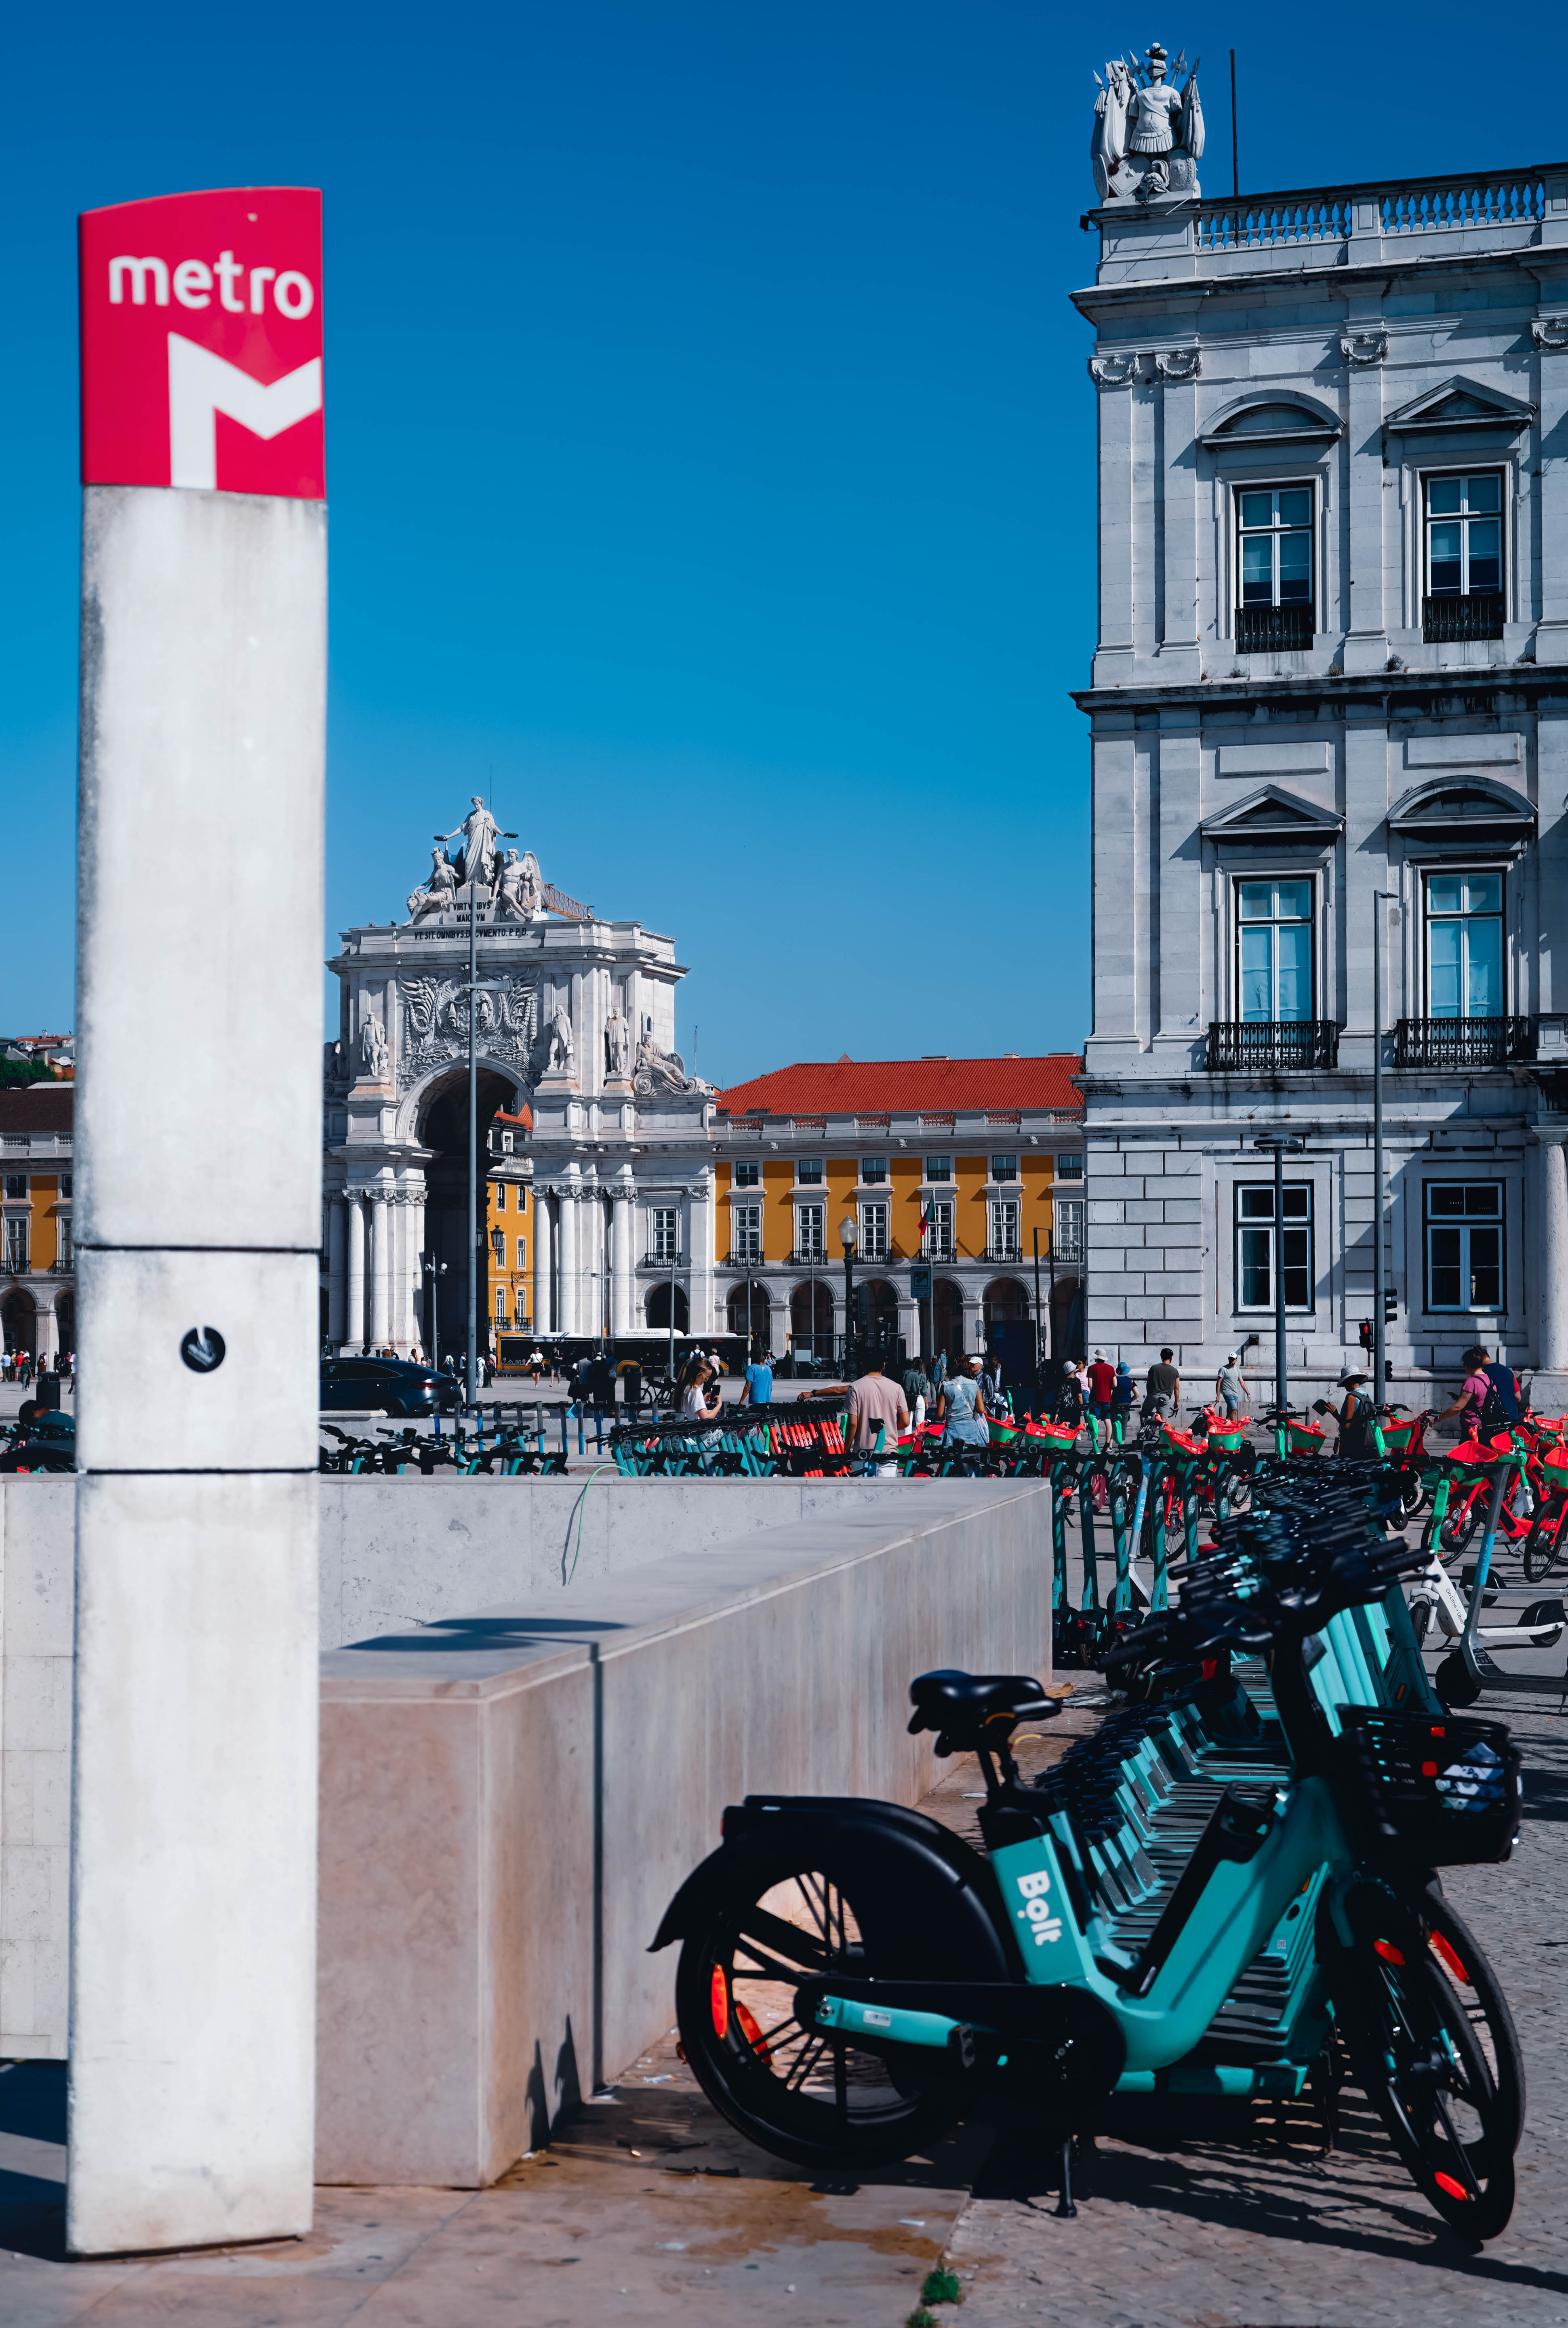
\includegraphics[width=\paperwidth,height=\paperheight]{src/Figures/Arriere_plan/Arriere_plan_Chap_2.jpg}
    }

% Rectangle
\AddToShipoutPictureBG*{
  \begin{tikzpicture}[remember picture,overlay]
    \node[fill=white, opacity=0.75, text width=\paperwidth, minimum height=12.25cm, anchor=north] 
    at ([yshift=-2cm]current page.north) {};
  \end{tikzpicture}
}

% Source
\AddToShipoutPictureFG*{
  \AtPageLowerRight{
    \raisebox{1cm}{
      \hspace{16cm}
      
\begin{tikzpicture}
        \node[fill=white, rounded corners=5pt, inner sep=5pt, align=center] {
          \tiny{Photographie~: \textcolor{blue}{Dylan Moinse (2023)}}
        };
      \end{tikzpicture}
    }
  }
}

    % ___________________________________________
    % Mini-sommaire
    \cleardoublepage
    \setcounter{tocdepth}{2}
    % Redéfinir le titre de la table des matières locale
    \renewcommand{\localcontentsname}{Table des matières du chapitre~2}
\localtableofcontents

% Réinitialiser numérotation section
\setcounter{section}{0}

    % ___________________________________________
    % Graphical abstract
    \newpage
\section*{Points clés du chapitre~2
    \label{chap2:graphical-abstract}
    }
    \markright{Préambule du chapitre}{}

\begin{figure}[h!]\vspace*{4pt}
        \caption*{}
        \label{graphical-abstract-chap2}
        \centerline{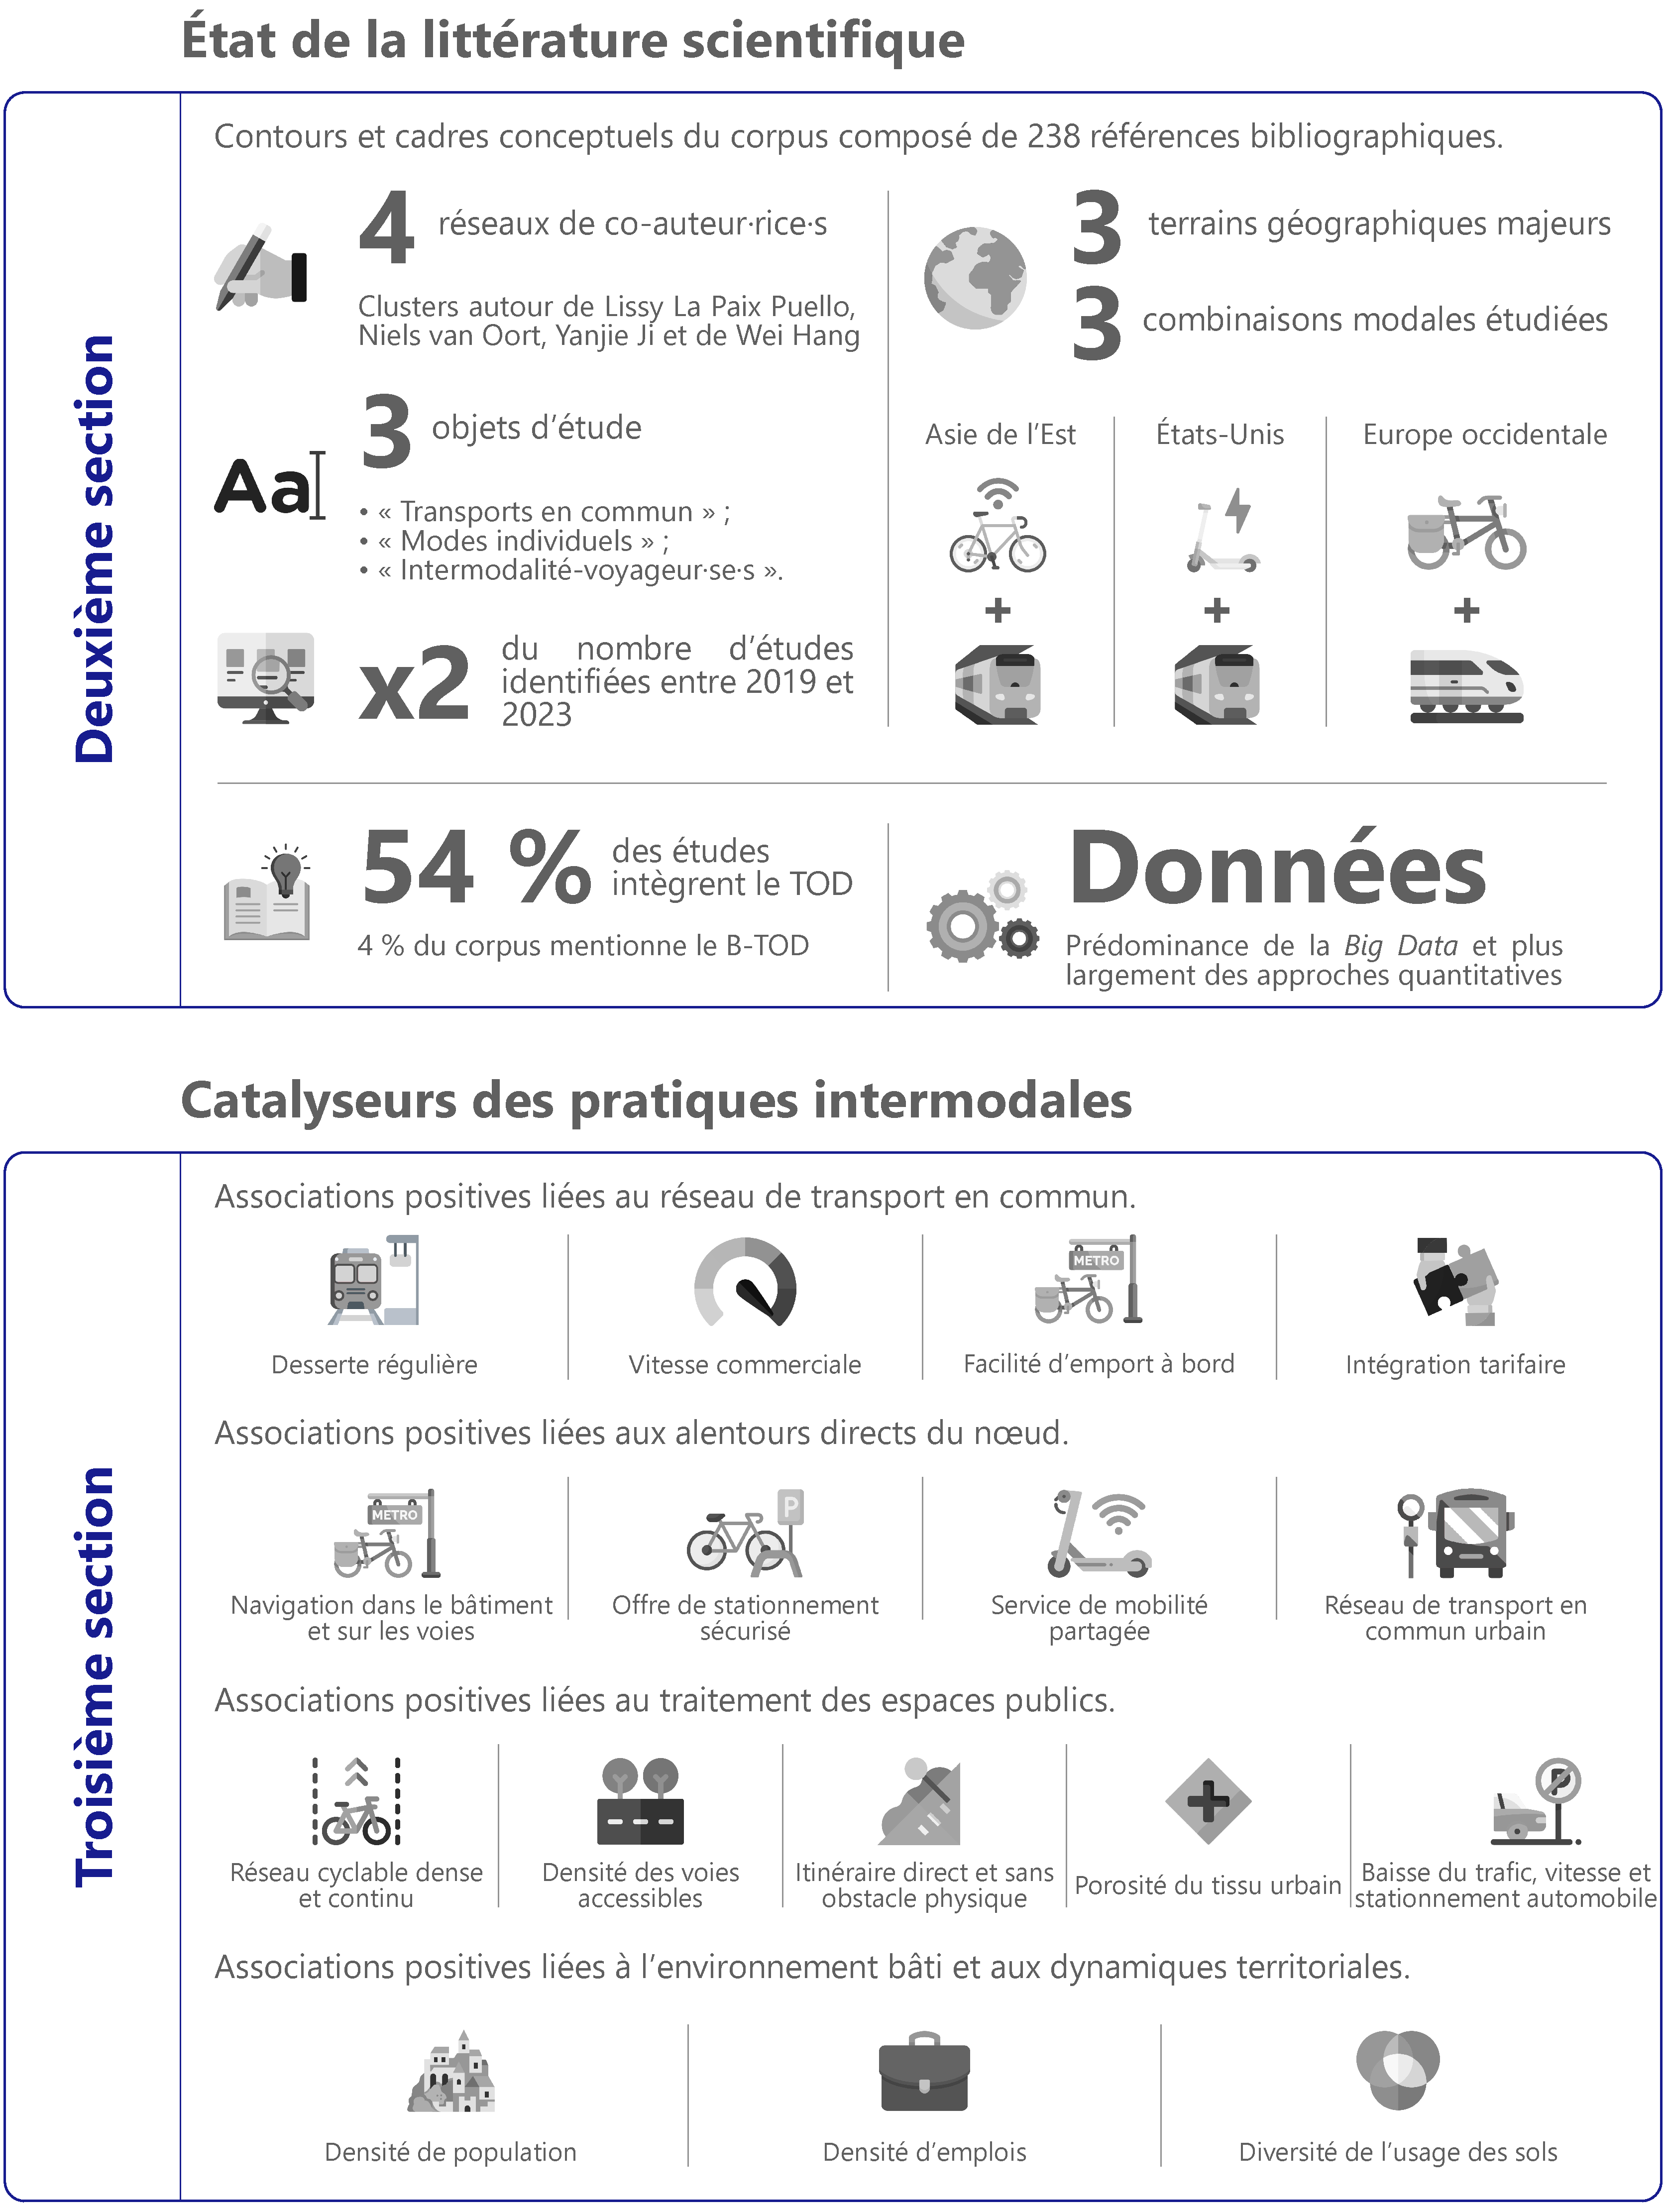
\includegraphics[width=1\columnwidth]{src/Figures/Graphical-abstract/FR_Graphical_abstract_chap2.pdf}}
        \vspace{5pt}
    \end{figure}

    % ___________________________________________
    % Préambule
    \newpage
    \begin{tcolorbox}[colback=white!5!white,
                      colframe=blue!75!blue,
                      title=
                      \bigskip
                      \center{\textbf{Préambule du chapitre~2}}
                      \\
                      \raggedright{\small{Chapitre composé de \pagedifference{chap2:titre}{chap3:titre} pages, dont \pagedifference{chap2:bibliographie}{chap3:titre} pages de bibliographie}}
                      \bigskip]
\Large{\textbf{\textcolor{blue}{Résumé~:}}}
    \\
    \small{
Le présent chapitre s'attache à apporter une vue d'ensemble de la recherche actuelle sur la conception d'un \acrfull{TOD} promouvant et promu par la mobilité individuelle légère. Cette étude bibliométrique et cette analyse bibliographique se présentent sous la forme d'une \acrfull{RSL} en constituant un recueil de 238 publications scientifiques. Dans la perspective de dresser un état des connaissances sur le \acrshort{B-TOD} et sur le \acrshort{M-TOD}, ce chapitre privilégie l'adoption de la \acrshort{RSL} en raison de sa capacité à conduire une analyse exhaustive de la littérature scientifique relative à ce sujet de recherche.%%Rédigé%%
    \\
L'élaboration de ce corpus a impliqué un processus de sélection d'articles scientifiques, d'articles de colloque, de chapitres d'ouvrages, de mémoires et de rapports de recherche diffusés en anglais et en français. Ces travaux académiques ont été examinés en se référant à des critères prédéfinis dans le but d'identifier l'ensemble des recherches abordant spécifiquement l'articulation entre la mobilité individuelle légère et les transports en commun (voir la \hyperref[chap2:protocole-methodologique-rsl]{section~1}, page~\pageref{chap2:protocole-methodologique-rsl}).%%Rédigé%%
    \\
Dans un premier temps, cette étude bibliographique a questionné les contextes temporels, géographiques et institutionnels influençant le champ de recherche sur le \acrshort{M-TOD}, ainsi que les cadres conceptuels et méthodologiques définis pour évaluer ce modèle urbain (voir la \hyperref[chap2:analyse-documentation-rsl]{section~2}, page~\pageref{chap2:analyse-documentation-rsl}). L'analyse de la répartition chronologique et spatiale des références bibliographiques a révélé un intérêt croissant pour l'intermodalité-voyageur·se·s, centré autour de trois pays à une échelle locale, avec des formes de combinaison modale qui évoluent dans le temps. La méthodologie adoptée tend vers l'élaboration d'analyses géostatistiques et de modélisations, facilitées par le développement des outils informatiques et de la \textsl{Big Data}.%%Rédigé%%
    \\
La troisième partie de ce chapitre se consacre à l'analyse des enseignements tirés des études examinées, en prêtant une attention particulière aux diverses composantes du \acrshort{B-TOD} et du \acrshort{M-TOD}, conceptualisées sous le terme des \Guillemets{\acrfull{7Ds}}~(voir la \hyperref[chap2:caracterisation-btod-environnement-urbain-choix-individuels]{section~3}, page~\pageref{chap2:caracterisation-btod-environnement-urbain-choix-individuels}). La caractérisation du \acrshort{M-TOD} a révélé tant des similitudes que des divergences, soulignant une association positive avec la densité de population et des emplois, la diversité de l'usage des sols, le traitement des espaces publics ou encore la qualité de l'offre en transport en commun. Divers impacts sur les comportements de mobilité, principalement pendulaires, et sur l'environnement ont été identifiés, tels qu'une diminution du bilan carbone, une amélioration de l'\gls{accessibilité} vers les destinations par une plus grande partie de la population, mais également l'existence d'inégalités sociales en termes d'accessibilité.%%Rédigé%%
    \\
En dernier lieu, la \acrshort{RSL} ouvre la voie à une lecture critique sur les lacunes présentes dans la littérature scientifique et sur les défis du \acrshort{M-TOD} (voir la \hyperref[chap2:conclusion]{conclusion du chapitre}, page~\pageref{chap2:conclusion}).%%Rédigé%%
    }
    \tcblower
\Large{\textbf{\textcolor{blue}{Mots-clés~:}}}
    \\
    \small{
Analyse bibliométrique~;
Analyse des réseaux~;
Caractéristiques socio-économiques~;
Caractéristiques urbaines~;
Cartographie scientifique~;
Comportements de mobilité~;
Impacts~;
Lecture critique du M-TOD~;
Mise en perspective internationale~;
Revue systématique de la littérature
    }
    \end{tcolorbox}

    % ___________________________________________
    % 2.*.
    \newpage
    \needspace{1\baselineskip} % Réserve de l'espace
    \addcontentsline{toc}{section}{Introduction du chapitre~2}
    \sectionheader{Introduction du chapitre}
\section*{Introduction du chapitre~2
    \label{chap2:introduction}
    }
    \markright{Introduction du chapitre~2}{}

    % Citation
    \begin{displayquote}
\Guillemets{\textsl{En complément des innovations au sein des modes de transport, les forces et faiblesses identifiées précédemment définissent également l'étendue des combinaisons possibles entre différents modes de déplacement. L'une de ces combinaisons est celle entre des modes de déplacement offrant un accès spatial relativement plus élevé grâce à leur vitesse, avec des modes plus lents présentant d'autres avantages.} [\dots] \textsl{Les combinaisons entre des modes de déplacement rapides (comme les trains) et des modes non motorisés, en particulier le \gls{vélo}, permettent une vitesse globale élevée de porte-à-porte, reliant ainsi efficacement une multitude de lieux d'origine et de destination. La combinaison train-vélo est particulièrement efficace~: le train est bien plus rapide que les autres transports en commun, et le vélo allie un accès ubiquitaire à des vitesses relativement élevées (supérieures à la marche, mais souvent aussi compétitives que le bus conventionnel ou le tramway, et même l'automobile dans certains environnements urbains). Dans les pays où l'infrastructure cyclable et les services ferroviaires sont étendus~–~comme aux Pays-Bas~–~cette combinaison modale est tellement développée qu'elle peut être considérée comme un mode de déplacement à part entière, et dans de nombreux contextes urbains, directement compétitive avec la voiture.} [\dots] \textsl{De plus, la combinaison train-vélo pourrait s'intégrer dans un système hybride, à la fois rapide et flexible, et donc pleinement compétitif avec la voiture.} [\dots] \textsl{Ce type de comportement multimodal est actuellement limité, mais pourrait se généraliser à l'avenir.} [\dots] \textsl{Et si un tel comportement hybride et adaptatif conjugué à un tel système de transport devenaient dominants~?}}\footnote{
    \Guillemets{\textsl{Next to innovations within transport modes, the strengths and weaknesses identified above also define the scope for transport mode combinations between transport modes. One such combination is between transport modes that give a relatively higher spatial access because of their speed with slower modes that have some other advantage.} [\dots] \foreignlanguage{english}{\textsl{Combinations between fast transit (such as trains) and non-motorized modes, particularly the bike, allow overall high door-to-door speed between virtually ubiquitous origin destinations. The train-bike combination is a particularly strong one: the train is much faster than other public transport, and the bike combines ubiquitous access with relatively high speeds (higher than walking but often also competitive with conventional buses or trams, and in certain environments even cars). In countries where both biking infrastructure and railway services are extensive~–~such as the Netherlands~–~this combination is so developed that it can be considered a transport mode in itself, and in many contexts directly competitive with the car.}} [\dots] \textsl{But also, the train-bike combination might integrate into a hybrid system which is both fast and flexible, and thus fully competitive with the car.} [\dots] \textsl{This type of multi-modal behaviour is now limited, but could become generalized in the future.} [\dots] \textsl{What if such a hybrid, highly adaptive behaviour and transportation system became dominant?}} \textcolor{blue}{\autocite[80-81, 220]{bertolini_planning_2017}}\index{Bertolini, Luca|pagebf}.} [traduction libre]

\textcolor{blue}{Luca} \textcolor{blue}{\textcite[80-81, 220]{bertolini_planning_2017}}\index{Bertolini, Luca|pagebf}. \foreignlanguage{english}{\textsl{Planning the Mobile Metropolis: Transport for People, Places and the Planet}}, Ed. Red Globe Press, Londres, 253~p. ISBN~: \href{https://search.worldcat.org/fr/title/1004435849}{978-0-230-30877-0}
    \end{displayquote}

    % Introduction
\lettrine[lines=3, findent=8pt, nindent=0pt]{\lettrinefont C}{e} chapitre vise à présenter l'état des connaissances actuelles qui aborde la redéfinition du \acrfull{TOD} en lien avec le regain d'intérêt pour la mobilité individuelle légère, dans la perspective de définir le concept de \acrfull{B-TOD} élargi par la mobilité individuelle légère. Afin de recueillir, d'analyser et de mettre en perspective les recherches traitant de ce sujet de recherche, une \acrfull{RSL} a été réalisée. Ainsi, seules les publications académiques diffusées en anglais ou en français et s'attachant à étudier cette forme d'\gls{intermodalité}-voyageur·se·s, d'un point de vue géographique et urbanistique, ont été incluses dans cette analyse bibliographique.%%Rédigé%%

    % Justification B-TOD / M-TOD
À la lumière du potentiel de la mobilité individuelle légère d'étendre l'\gls{accessibilité intermodale} des nœuds de \gls{transport en commun} \textcolor{blue}{\autocite[118]{cottrell_transforming_2007}}\index{Cottrell, Wayne~D.|pagebf}, l'objectif sous-jacent de cette analyse critique de la littérature scientifique relative au concept émergent du \acrfull{M-TOD} est de regrouper et de mieux comprendre la façon dont cette combinaison modale peut favoriser une conception urbaine propice au développement de modes de déplacement alternatifs. En partant du constat que l'association des transports en commun avec la mobilité individuelle légère, au même titre que la marche combinée, représente la forme d'intégration la plus efficace \textcolor{blue}{\autocite[50]{sebban_complementarite_2003, yang_study_2013}}\index{Sebban, Annie-Claude|pagebf}\index{Yang, Rongrong|pagebf}\index{Yan, Hai|pagebf}\index{Xiong, Wen|pagebf}\index{Liu, Tao|pagebf}, aussi bien sur le plan économique, social qu'environnemental — trois dimensions valorisées par le \acrshort{TOD} \textcolor{blue}{\autocite[85]{cervero_bike-and-ride_2013}}\index{Cervero, Robert|pagebf}\index{Caldwell, Benjamin|pagebf}\index{Cuellar, Jesus|pagebf} — la question de recherche abordée par cette \acrshort{RSL} est double. Il s'agit de justifier l'intégration de la mobilité individuelle légère aux systèmes de transport en commun par opposition à d'autres formes d'intermodalité telles que les parcs relais, tout en identifiant les défis inhérents au modèle urbain du \acrshort{M-TOD}.%%Rédigé%%

    % Justification RSL
L'intérêt d'entreprendre une \acrshort{RSL} réside dans sa capacité à rassembler, évaluer et synthétiser les connaissances existantes sur un sujet de recherche complexe qui mêle deux objets d'étude interdisciplinaires faisant non seulement appel à l'urbanisme et à la mobilité, mais également à une multitude de disciplines s'intéressant aux systèmes urbains, aux infrastructures et aux populations. La démarche innovante de la \acrshort{RSL} se distingue de la revue de littérature classique par sa recherche d'objectivité accrue, son objectif d'exhaustivité, la formulation de questions précises et la meilleure transparence des étapes composant le cheminement. Si cette méthode est principalement utilisée dans les sciences exactes, la \acrshort{RSL} tend à démontrer son efficacité dans les \acrfull{SHS} par le biais d'ajustements progressifs. Ainsi, l'élaboration d'une telle méthode sur un sujet de recherche original et récent présente plusieurs avantages. Elle permet d'identifier et d'évaluer les études existantes en adoptant une vision globale et nette de l'état des connaissances scientifiques, de repérer les tendances émergentes et l'évolution des recherches, ainsi que de déterminer les aspects insuffisamment explorés. Par conséquent, la \acrshort{RSL} permet également d'orienter les recherches futures, à l'instar de la présente recherche doctorale.%%Rédigé%%

    % Annonce du plan 1
Nous procéderons tout d'abord à une présentation détaillée du protocole méthodologique destiné à composer le corpus académique (\hyperref[chap2:protocole-methodologique-rsl]{section~1}, page~\pageref{chap2:protocole-methodologique-rsl}), qui inclura la formulation des questions de recherche (\hyperref[chap2:formulation-questions-recherche]{sous-section~1.1}, page~\pageref{chap2:formulation-questions-recherche}), la stratégie de recherche documentaire (\hyperref[chap2:strategie-recherche-documentaire]{sous-section~1.2}, page~\pageref{chap2:strategie-recherche-documentaire}), les processus de sélection des publications scientifiques (\hyperref[chap2:selection-publications-scientifiques]{sous-section~1.3}, page~\pageref{chap2:selection-publications-scientifiques}) et d'extraction des données récoltées ainsi que les points examinés (\hyperref[chap2:extraction-donnees-aspects-consideres]{sous-section~1.4}, page~\pageref{chap2:extraction-donnees-aspects-consideres}).%%Rédigé%%

    % Annonce du plan 2
Une fois la méthodologie exposée, nous soulignerons les caractéristiques de la littérature scientifique et des pratiques de recherche sur ce sujet (\hyperref[chap2:analyse-documentation-rsl]{section~2}, page~\pageref{chap2:analyse-documentation-rsl}), à travers l'analyse des métadonnées issues de la documentation (\hyperref[chap2:etat-litterature-scientifique-internationale-btod]{sous-section~2.1}, page~\pageref{chap2:etat-litterature-scientifique-internationale-btod}) et des cadres conceptuels et méthodologiques des références bibliographiques (\hyperref[chap2:cadres-conceptuels-methodologiques]{sous-section~2.2}, page~\pageref{chap2:cadres-conceptuels-methodologiques}).%%Rédigé%%

    % Annonce du plan 3
Le troisième temps de cette \acrshort{RSL} sera consacré à la présentation synthétique des \Guillemets{\acrfull{7Ds}}~et des principaux enseignements qui servent de principes directeurs pour le TOD (\hyperref[chap2:caracterisation-btod-environnement-urbain-choix-individuels]{section~3}, page~\pageref{chap2:caracterisation-btod-environnement-urbain-choix-individuels}), en interrogeant l'association entre l'intégration de la mobilité individuelle légère et l'influence de la densité de population (\hyperref[chap2:densite-population]{sous-section~3.1}, page~\pageref{chap2:densite-population}), de la diversité fonctionnelle (\hyperref[chap2:diversite-fonctionnelle]{sous-section~3.2}, page~\pageref{chap2:diversite-fonctionnelle}), du traitement des espaces publics (\hyperref[chap2:traitement-espaces-publics]{sous-section~3.3}, page~\pageref{chap2:traitement-espaces-publics}), de l'accessibilité intermodale (\hyperref[chap2:accessibilite-intermodale]{sous-section~3.4}, page~\pageref{chap2:accessibilite-intermodale}), des distances vers et depuis les nœuds de transport en commun (\hyperref[chap2:distances-premiers-derniers-km]{sous-section~3.5}, page~\pageref{chap2:distances-premiers-derniers-km}), de la gestion de la demande de mobilité (\hyperref[chap2:gestion-demande-mobilite]{sous-section~3.6}, page~\pageref{chap2:gestion-demande-mobilite}), des caractéristiques socio-démographiques des usager·ère·s (\hyperref[chap2:sociodemographie-usagers]{sous-section~3.7}, page~\pageref{chap2:sociodemographie-usagers}), des comportements de mobilité (\hyperref[chap2:comportements-mobilite]{sous-section~3.8}, page~\pageref{chap2:comportements-mobilite}) et des impacts de ces pratiques intermodales sur les systèmes de mobilité et les systèmes urbains (\hyperref[chap2:impacts-systemes-urbain-mobilite]{sous-section~3.9}, page~\pageref{chap2:impacts-systemes-urbain-mobilite}).%%Rédigé%%

    % Annonce du plan 4
En guise de conclusion, nous avancerons les pistes de recherche futures portant sur l'intégration de la mobilité individuelle légère au \acrshort{TOD} et qui viendront alimenter cette thèse de doctorat (\hyperref[chap2:conclusion]{conclusion du chapitre~2}, page~\pageref{chap2:conclusion}).%%Rédigé%%

    % ___________________________________________
    % 2.1.
    \newpage
    \needspace{1\baselineskip} % Réserve de l'espace
    \sectionheader{Méthodologie de la revue systématique de la littérature}
\section{Protocole méthodologique de la revue systématique de la littérature
    \label{chap2:protocole-methodologique-rsl}
    }
    
    % Etat de l'art RSL
La procédure méthodologique sous-tendant l'élaboration d'une \acrshort{RSL} est en constante évolution en raison de sa genèse relativement tardive dans les champs des \acrshort{SHS} et des discussions actuelles sur les limites méthodologiques qui lui sont associées. La \acrshort{RSL} conduite dans le cadre de ce chapitre s'inscrit dans le sillage des techniques énoncées dans l'article de référence consacré à la réalisation d'une \acrshort{RSL} thématique et qualitative, dans une revue scientifique médicale, sous la plume de \textcolor{blue}{\textcite[3-7]{thomas_methods_2008}}\index{Thomas, James|pagebf}\index{Harden, Angela|pagebf}. En tenant compte des nuances dans la réalisation d'une \acrshort{RSL} selon les disciplines \textcolor{blue}{\autocite[738]{padeiro_transit-oriented_2019}}\index{Padeiro, Miguel|pagebf}\index{Louro, Ana|pagebf}\index{Costa, Nuno Marques de|pagebf}, le protocole méthodologique développé repose sur les enseignements tirés de différentes \acrshort{RSL} examinant le \acrshort{TOD} et la mobilité individuelle légère. À ce titre, la méthode construite se nourrit des techniques et des réflexions issues de diverses \acrshort{RSL}, l'une portant sur les liens entre le \acrshort{TOD} et la gentrification \textcolor{blue}{\autocite[738]{padeiro_transit-oriented_2019}}\index{Padeiro, Miguel|pagebf}\index{Louro, Ana|pagebf}\index{Costa, Nuno Marques de|pagebf}, l'autre au sujet de l'intégration de la mobilité individuelle légère aux systèmes de transport en commun \textcolor{blue}{\autocite[4]{oeschger_micromobility_2020}}\index{Oeschger, Giulia|pagebf}\index{Carroll, Páraic|pagebf}\index{Caulfield, Brian|pagebf}. Plusieurs revues de littérature existantes ont également guidé la conception de notre \acrshort{RSL}, particulièrement celles examinant le vélo et la micro-mobilité électriques \textcolor{blue}{\autocite[3]{sengul_impacts_2021}}\index{Sengül, Buket|pagebf}\index{Mostofi, Hamid|pagebf}, les services de trottinettes électriques \textcolor{blue}{\autocite[4]{bozzi_shared_2021}}\index{Bozzi, Alberica Domitilla|pagebf}\index{Aguiléra, Anne|pagebf}, le choix des itinéraires cyclables \textcolor{blue}{\autocite[2]{pritchard_revealed_2018}}\index{Pritchard, John~P.|pagebf} et l'usage de la \textsl{Big Data} en lien avec la mobilité \textcolor{blue}{\autocite[36]{neilson_systematic_2019}}\index{Neilson, Alex|pagebf}\index{Indratmo|pagebf}\index{Daniel, Ben|pagebf}\index{Tjandra, Stevanus|pagebf}.%%Rédigé%%

    % Sélection
Par ailleurs, cette recherche bibliographique s'inspire du guide méthodologique destiné à produire une revue de littérature dans les domaines de l'aménagement urbain et de la mobilité, et adaptée par l'organisation académique nationale étasunienne \textcolor{blue}{\textcite{transportation_research_board_of_the_national_academies_literature_2015}}\index{Transportation Research Board@\textsl{Transportation Research Board}|pagebf}. Ce rapport identifie notamment six étapes principales visant à constituer une \acrshort{RSL}~: la définition du sujet de recherche enquêté (i), la sélection des librairies et des bases de données bibliographiques appropriées au sujet défini (ii), la formulation d'une expression à partir de mots-clés (iii), la définition des relations entre les termes pour développer une recherche avancée (iv), le contrôle de la collection de textes recueillie (v) puis l'organisation des données en vue de les analyser (vi) \textcolor{blue}{\autocite[2-18]{transportation_research_board_of_the_national_academies_literature_2015}}\index{Transportation Research Board@\textsl{Transportation Research Board}|pagebf}. De plus, le processus de sélection des publications scientifiques dans le cadre de cette \acrshort{RSL} embrasse les trois étapes établies par \textcolor{blue}{\textcite[2~544]{jain_systematic_2020}}\index{Jain, Deepshikha|pagebf}\index{Singh, Ekta|pagebf}\index{Ashtt, Rashmi|pagebf}~:
    \begin{customitemize}
        \item La phase initiale d'exclusion se caractérise par l'analyse des métadonnées, tirées des références bibliographiques et incluant à la fois le titre, le résumé et les mots-clés afférents, afin d'évaluer leur pertinence par rapport au sujet de recherche considéré~;
        \item La phase intermédiaire d'exclusion implique la lecture critique de l'introduction et de la conclusion de chaque document retenu afin de filtrer plus finement les publications scientifiques qui se rapportent aux objectifs de recherche fixés dans la \acrshort{RSL}~;
        \item La phase finale d'exclusion engage une lecture complète des études intégrées à la \acrshort{RSL} afin de garantir la qualité du processus de sélection.
    \end{customitemize}
En suivant ces trois séquences, le processus d'inclusion assure une approche méthodique en cernant les sources académiques pertinentes en lien avec le sujet de recherche spécifié.%%Rédigé%%

    % Avantages de la RSL
Vis-à-vis d'une revue de littérature conventionnelle, la \acrshort{RSL} acquiert le statut de \Guillemets{systématique}~lorsque celle-ci s'articule autour d'une question de recherche formulée, de l'identification de travaux en adéquation avec le sujet délimité et d'une explicitation claire de la méthodologie suivie. En ce sens, la \acrshort{RSL} détient plusieurs avantages comparatifs \textcolor{blue}{\autocite[2]{transportation_research_board_of_the_national_academies_literature_2015}}\index{Transportation Research Board@\textsl{Transportation Research Board}|pagebf}~:
    \begin{customitemize}
        \item La résolution de problèmes permise par la couverture complète des connaissances existantes sur une thématique précise~;
        \item La mise en confrontation d'études antérieures et concurrentes, de sorte à faciliter la compréhension du discours académique existant~;
        \item La validation des méthodes de recherche appliquées en questionnant la fiabilité des approches retenues~;
        \item La confirmation de la nécessité de poursuivre les recherches en mettant en évidence les domaines d'étude émergents~;
        \item L'orientation des efforts de recherche en offrant des perspectives qui viennent éclairer l'état des connaissances actuelles et dessiner des pistes prometteuses pour les futures initiatives de recherche.
    \end{customitemize}
À l'aide de ces avantages, la \acrshort{RSL} établit une base solide pour sonder la littérature scientifique, en contribuant à apporter une plus grande rigueur méthodologique, une analyse fine des recherches existantes et une feuille de route visant à guider les études ultérieures.%%Rédigé%%

    % 2.1.1.
    \needspace{1\baselineskip} % Réserve de l'espace
\subsection{Formulation des questions de recherche
    \label{chap2:formulation-questions-recherche}
    }
    
    % Questions et objectifs
L'objectif premier de cette \acrshort{RSL} est de fournir une compréhension approfondie des connaissances et des pratiques existantes en lien avec une fabrication urbaine orientée vers les transports en commun et reposant sur la mobilité individuelle légère, tout en déterminant les facteurs qui facilitent ou entravent la mise en œuvre du modèle urbain et en évaluant ses effets sur la mobilité et les territoires. À cet égard, la \acrshort{RSL} vise à examiner et à discuter, en premier lieu, du rôle du vélo au sein du modèle d'aménagement. Bien que l'intégration de ce mode de déplacement ait été envisagée dès la conceptualisation du \acrshort{TOD}, son potentiel semble demeurer sous-exploité. C'est dans cette optique que cette revue de littérature cherche à caractériser sa déclinaison, connue sous le nom de \acrshort{M-TOD}. Par ailleurs, nous nous employons à l'actualiser en y adjoignant l'exploration des options de \gls{micro-mobilité} émergente. Ces dernières, par leur caractère innovant, sont susceptibles d'interagir et de transformer à leur tour les fondements du \acrshort{M-TOD}.

Dans cette perspective, la grille de lecture suivante, centrée sur six questions de recherche, oriente la \acrshort{RSL}~:
    \begin{customitemize}
        \item Quels sont les facteurs urbains et les politiques publiques qui favorisent l'intégration du vélo et des options de micro-mobilité aux systèmes de transport en commun~? Réciproquement, cette forme de mobilité influence-t-elle les configurations territoriales~?
        \item Quels sont les effets de cette combinaison modale en termes de développement économique, de cohésion sociale et de respect de l'environnement~?
        \item Existe-t-il un périmètre pertinent pour définir un quartier de gare à partir de la mobilité individuelle légère~? La taille de ces aires d'influence varie-t-elle en fonction de certains paramètres~?
        \item Quelles sont les pratiques d'urbanisme et les modèles de gouvernance se révélant innovants et efficaces pour favoriser un tel développement urbain~?
        \item Peut-on considérer le \acrshort{M-TOD} comme un modèle urbain internationalement reconnu et réplicable~?
        \item Quels sont les principaux défis à relever dans la réflexion et l'application d'une stratégie \acrshort{M-TOD}~?
    \end{customitemize}%%Rédigé%%

    % 2.1.2.
    \needspace{1\baselineskip} % Réserve de l'espace
\subsection{Stratégie de recherche documentaire
    \label{chap2:strategie-recherche-documentaire}
    }

    % Recherche en ligne
La phase initiale de collecte des données se traduit par l'utilisation de recherches en ligne, à l'aide de bases de données bibliographiques offrant une couverture transdisciplinaire. Cette étape de recueil de la documentation veille à capturer et à répertorier un corpus exhaustif de références bibliographiques provenant de la littérature scientifique et de la littérature grise
    \footnote{
        Dans ce contexte, la littérature scientifique fait référence aux publications académiques évaluées par des pairs, incluant les articles publiés dans des revues scientifiques, actes de colloque, chapitres d'ouvrage et les mémoires de recherche. La littérature grise, telle que définie par l\acrfull{AFNOR} et la Convention luxembourgeoise sur la littérature grise, comprend des \Guillemets{\textsl{documents dactylographiés ou imprimés, souvent de nature provisoire, reproduits et distribués à moins d'un millier d'exemplaires, en dehors des circuits commerciaux de publication et de distribution}}~\textcolor{blue}{\autocite[30]{schopfel_comprendre_2015}}\index{Schöpfel, Joachim|pagebf}. La littérature grise couvre \Guillemets{\textsl{ce qui est produit par tous les niveaux de gouvernement, les universités, les entreprises et l'industrie, sous forme imprimée ou électronique, mais qui n'est pas contrôlé par l'édition commerciale}}~\textcolor{blue}{\autocite{national_grey_literature_collection_luxembourg_nodate}}\index{National Grey Literature Collection|pagebf}. Récemment, \textcolor{blue}{Joachim} \textcolor{blue}{\textcite[9]{schopfel_vers_2012}}\index{Schöpfel, Joachim|pagebf} a proposé une définition renouvelée de ce type de littérature, le considérant comme \Guillemets{\textsl{un document produit par le gouvernement, l'administration, l'éducation et la recherche, l'entreprise et l'industrie, sous forme imprimée ou électronique, protégé par des droits de propriété intellectuelle, d'une qualité suffisante pour être collecté et préservé par une bibliothèque ou une archive institutionnelle, et qui n'est pas contrôlé par l'édition commerciale}}.
}. Dans le cadre de cette \acrshort{RSL}, les recherches en ligne intègrent les articles scientifiques, les actes de colloque, les chapitres d'ouvrage, les mémoires de recherche en master ou en doctorat et les rapports de recherche publics. Cependant, elles excluent, entre autres, les prépublications scientifiques, documents techniques ou politiques, rapports d'étude privés, déclarations publiques ou encore les bulletins d'information. Il faut noter que l'inventaire de la bibliographie liée au \acrshort{M-TOD} a été initialement réalisé entre le 3 et le 8 décembre 2021. Par la suite, eu égard à la dimension naissante de ce sujet, une mise à jour de la collecte des données a été effectuée entre le~10~et le~13~avril~2023 afin d'inclure les publications les plus récentes.%%Rédigé%%

    % Etape de recherche en ligne
La collecte des données pour cette \acrshort{RSL} s'est manifestée par une \acrfull{Recherche EN}, ou \(R_{EN}\), et une \acrfull{Recherche FR}, ou \(R_{FR}\), en exploitant diverses plates-formes en ligne jouissant d'une reconnaissance solide dans la sphère académique. Les ressources académiques citées ci-après ont été sélectionnées du fait de leur couverture étendue, de leur accessibilité et de leur fiabilité. De surcroît, ces bases de données numériques facilitent l'identification, l'indexation et l'exportation vers des logiciels de gestion de références bibliographiques d'un large éventail de références scientifiques, notamment grâce aux outils de recherche avancée intégrés.%%Rédigé%%

    % Figure RSL - Echantillonnage
    \begin{figure}[h!]\vspace*{4pt}
        \caption{Diagramme de flux représentant le processus de sélection des publications scientifiques intégrées dans la revue systématique de la littérature.}
        \label{fig-chap2:diagramme-flux-selection-publications-rsl}
        \centerline{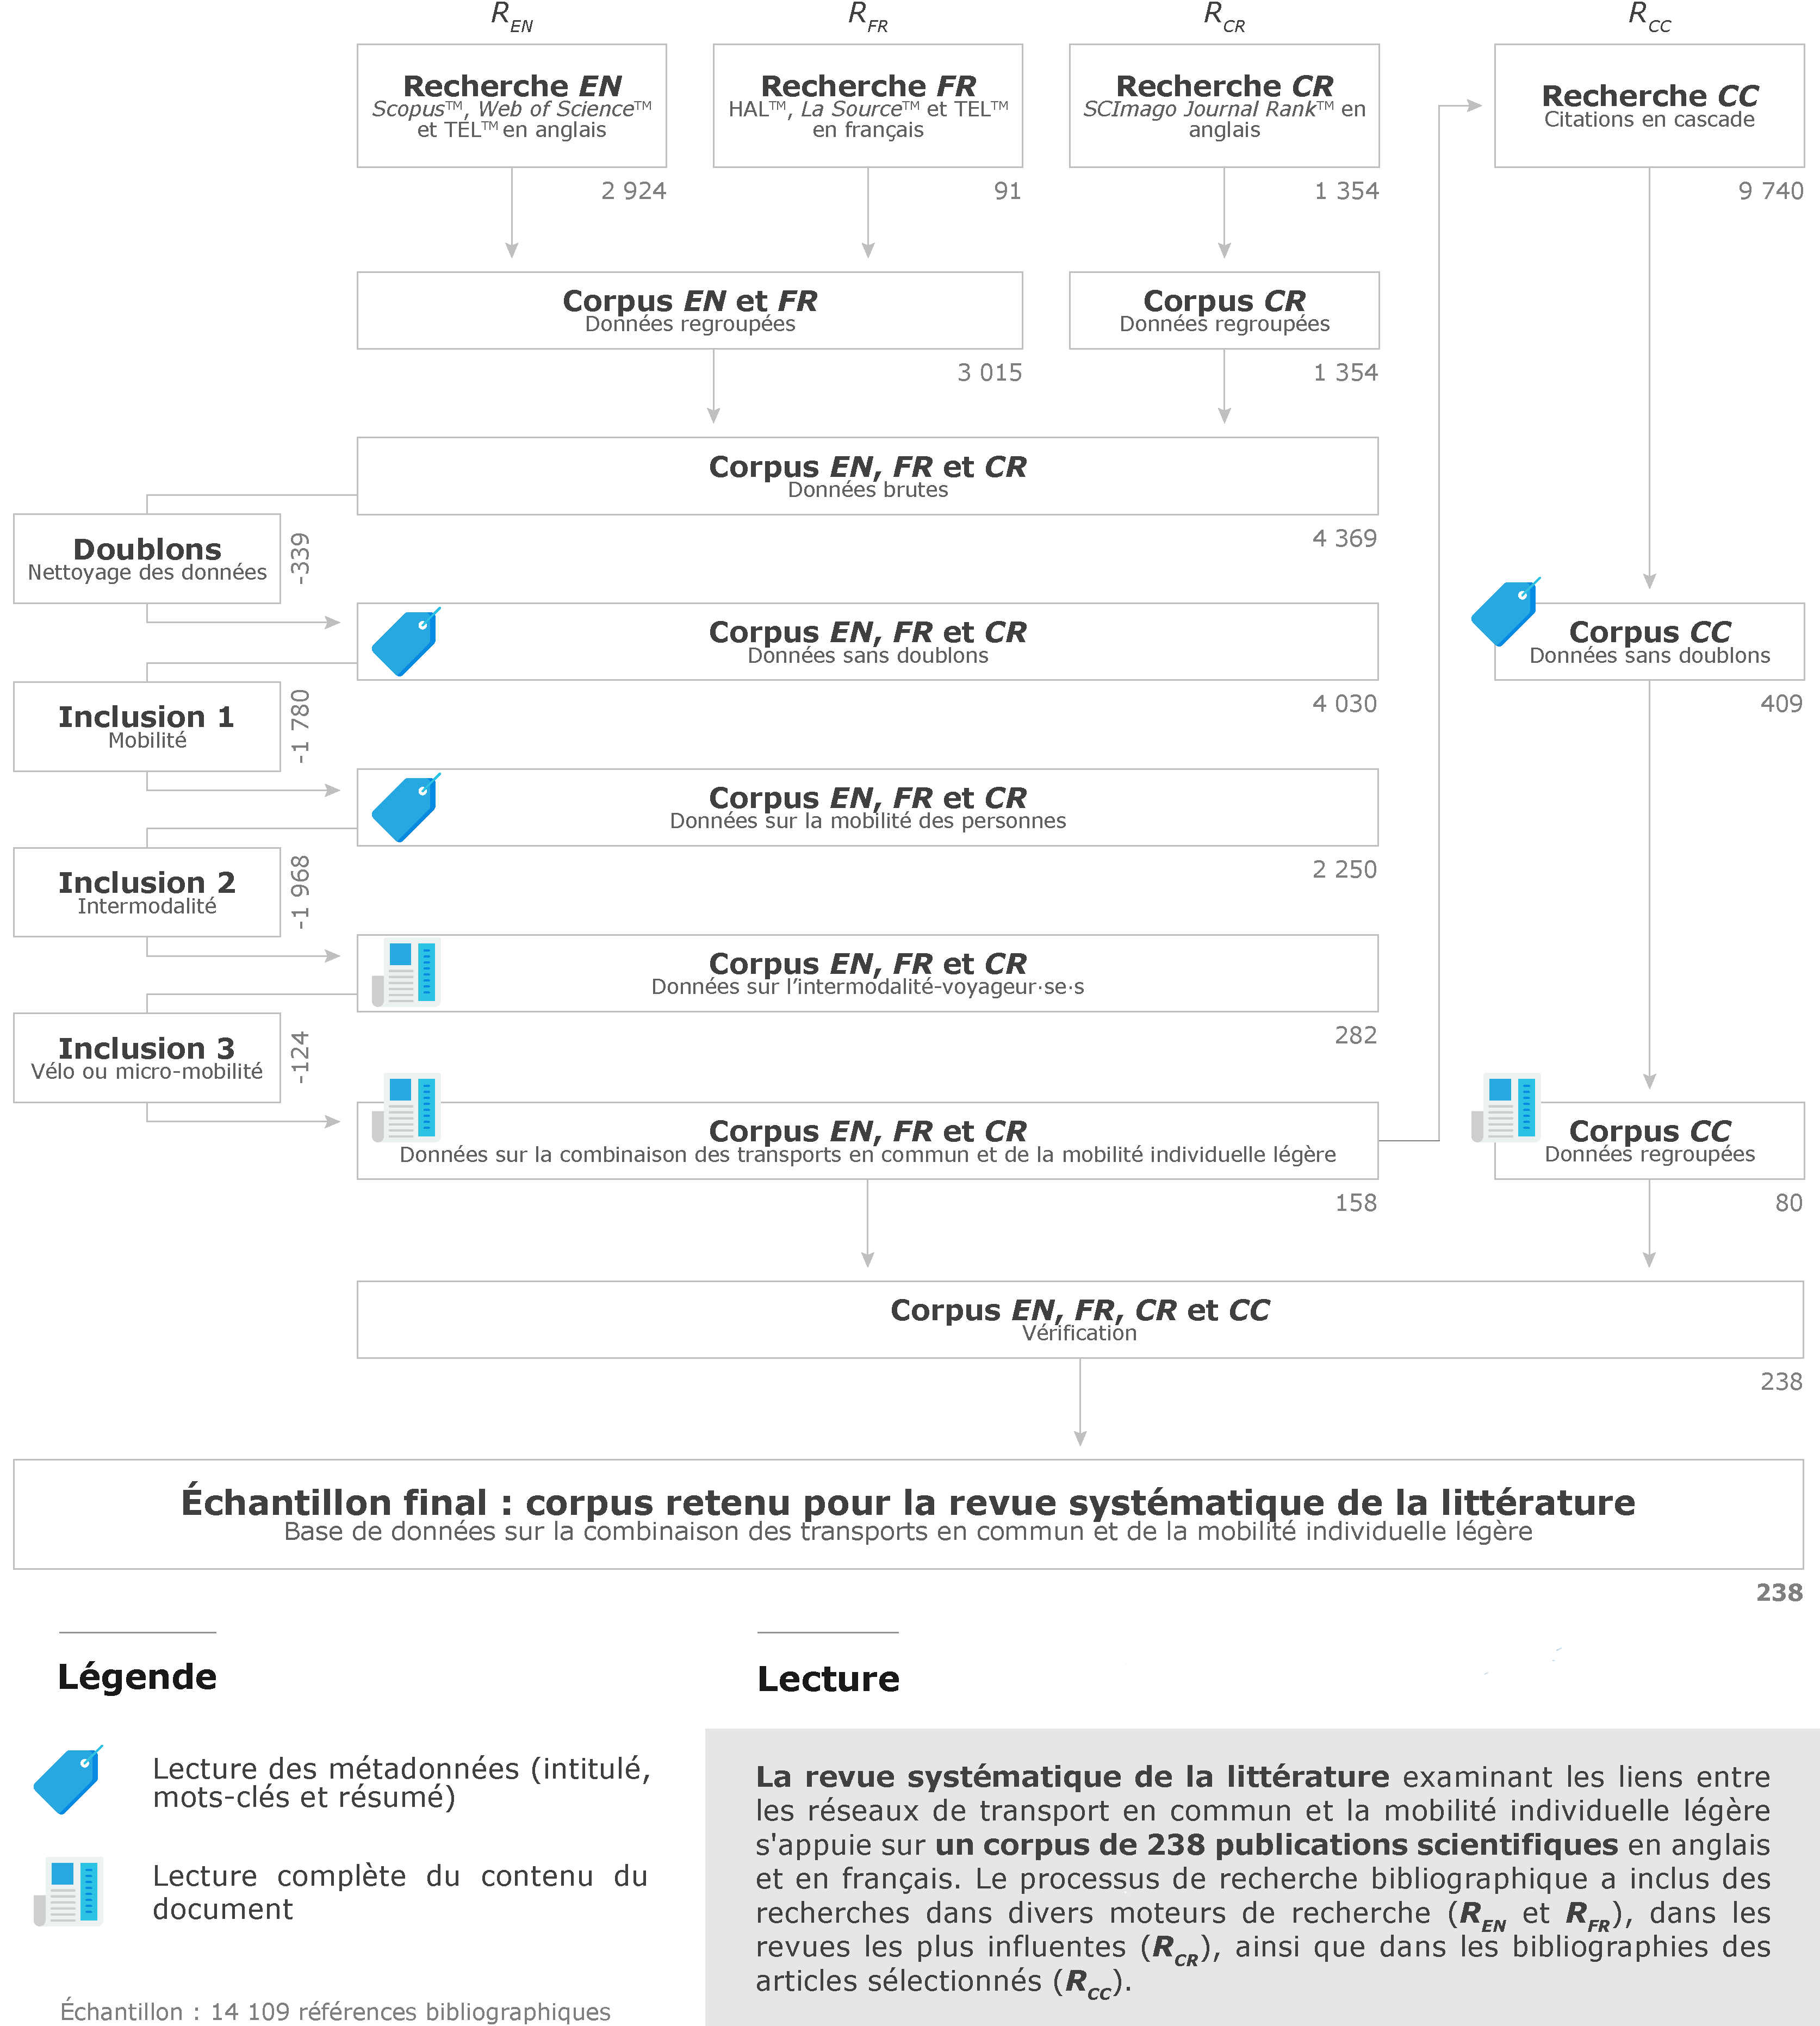
\includegraphics[width=1\columnwidth]{src/Figures/Chap-2/FR_RSL_Diagramme_flux_selection_publications.pdf}}
        \vspace{5pt}
        \begin{flushright}\scriptsize{
        Auteur~: \textcolor{blue}{Dylan Moinse (2023)}
        }\end{flushright}
    \end{figure}

    % Recherches EN+FR
Dans le premier cas, nous avons interrogé les bases de données documentaires \Marque{Scopus}~et \Marque{Web of Science}\footnote{
    \textsl{Scopus} (\url{www.scopus.com}) et \textsl{Web of Science} (\url{www.webofscience.com}) sont des plates-formes bibliographiques en ligne couramment utilisées dans le domaine de la recherche académique. \textsl{Scopus} est développé par \Marque{Elsevier}, une société spécialisée dans l'édition scientifique, tandis que \textsl{Web of Science} est une collection de travaux académiques gérée par \Marque{Clarivate Analytics}.
}. En complément, le serveur \Marque{TEL}\footnote{
    \textsl{theses.fr} (\url{www.theses.fr}) est une plate-forme d'archives pour les thèses de doctorat, offrant régulièrement un accès en ligne à des ressources académiques produites par des docteur·e·s.
} a été consulté afin d'élargir la recherche aux thèses de doctorat soumises en anglais. Dans un second temps, la recherche bibliographique en français s'est appuyée sur le portail \Marque{HAL}\footnote{
    \textsl{Hyper Article en Ligne} (\url{https://hal.science/}) est un portail d'archives ouvert qui facilite le dépôt, la diffusion et la consultation de documents scientifiques. Ce portail a été développé par le \acrfull{CCSD} du \acrfull{CNRS}. \textsl{HAL} permet aux chercheurs et aux institutions de diffuser gratuitement leurs travaux de recherche afin de faciliter l'accès libre et la visibilité des travaux de recherche.
}, la plate-forme \Marque{La Source}\footnote{
    \textsl{La Source} (\url{https://bibliotheque.enpc.fr}) est la bibliothèque en ligne développée par l'\textsl{École des Ponts Paristech}, conçue pour faciliter l'accès aux ressources scientifiques disponibles sur sa plate-forme en ligne.
} et une nouvelle fois sur le serveur \textsl{TEL}. La \Guillemets{\acrshort{Recherche EN}}~a abouti à la compilation de 2~924 publications scientifiques, tandis que la \Guillemets{\acrshort{Recherche FR}}~a permis d'y ajouter 91 références, après réactualisation de la collection en avril 2023. Ainsi, cette première étape de recherche en ligne a formé un corpus de 3 015 documents, désigné sous le nom de \Guillemets{Corpus EN et FR}~(voir l'\hyperref[fig-chap2:diagramme-flux-selection-publications-rsl]{illustration~\ref{fig-chap2:diagramme-flux-selection-publications-rsl}}, page~\pageref{fig-chap2:diagramme-flux-selection-publications-rsl}).%%Rédigé%%

    % Tableau revues scientifiques
% Tableau types de quartier de gare
%%Rédigé%%
        \begin{table}[h!]
    \centering
    \renewcommand{\arraystretch}{1.5}
    \resizebox{\columnwidth}{!}{
    \begin{tabular}{p{0.07\columnwidth}p{0.1\columnwidth}p{0.7\columnwidth}p{0.13\columnwidth}}
        %\hline
    \rule{0pt}{15pt} \small{\textbf{\textcolor{blue}{Rang}}} & \small{\textbf{\textcolor{blue}{Étiquette}}} & \small{\textbf{\textcolor{blue}{Revue scientifique}}} & \small{\textbf{\textcolor{blue}{Indice \acrshort{SJR}}}}\\
        \hline
    \multicolumn{4}{l}{\small{\textbf{\textcolor{blue}{Transports (2023)}}}}\\
\small{1} & \small{\(SMG_{T1}\)} & \small{\textsl{Analytic Methods in Accident Research}} & \small{4,8}\\
\small{2} & \small{\(SMG_{T2}\)} & \small{\textsl{Tourism Management}} & \small{3,4}\\
\small{3} & \small{\(SMG_{T3}\)} & \small{\textsl{Transportation Research Part B: Methodological}} & \small{3,4}\\
\small{4} & \small{\(SMG_{T4}\)} & \small{\textsl{Journal of Travel Research}} & \small{3,3}\\
\small{5} & \small{\(SMG_{T5}\)} & \small{\textsl{Transportation Research Part C: Emerging Technologies}} & \small{3,2}\\
\small{6} & \small{\(SMG_{T6}\)} & \small{\textsl{Transport Reviews}} & \small{3,1}\\
\small{7} & \small{\(SMG_{T7}\)} & \small{\textsl{Transportation Research Part E: Logistics and Transportation}} & \small{2,8}\\
\small{8} & \small{\(SMG_{T8}\)} & \small{\textsl{Transportation Science}} & \small{2,8}\\
\small{9} & \small{\(SMG_{T9}\)} & \small{\textsl{Journal of Public Transportation}} & \small{2,3}\\
\small{10} & \small{\(SMG_{T10}\)} & \small{\textsl{Transportation Research, Part A: Policy and Practice}} & \small{2,2}\\
        \hline
    \multicolumn{4}{l}{\small{\textbf{\textcolor{blue}{Études urbaines (2023)}}}}\\
\small{1} & \small{\(SMG_{U1}\)} & \small{\textsl{Nature Sustainability}} & \small{5,8}\\
\small{2} & \small{\(SMG_{U2}\)} & \small{\textsl{Journal of Urban Economics}} & \small{2,8}\\
\small{3} & \small{\(SMG_{U3}\)} & \small{\textsl{Journal of Public Transportation}} & \small{2,3}\\
\small{4} & \small{\(SMG_{U4}\)} & \small{\textsl{Transportation Research Interdisciplinary Perspectives}} & \small{2,1}\\
\small{5} & \small{\(SMG_{U5}\)} & \small{\textsl{Landscape and Urban Planning}} & \small{1,9}\\
\small{6} & \small{\(SMG_{U6}\)} & \small{\textsl{Urban Studies}} & \small{1,9}\\
\small{7} & \small{\(SMG_{U7}\)} & \small{\textsl{International Journal of Urban and Regional Research}} & \small{1,9}\\
\small{8} & \small{\(SMG_{U8}\)} & \small{\textsl{Journal of the American Planning Association}} & \small{1,8}\\
\small{9} & \small{\(SMG_{U9}\)} & \small{\textsl{Computers, Environment and Urban Systems}} & \small{1,7}\\
\small{10} & \small{\(SMG_{U10}\)} & \small{\textsl{Cities}} & \small{1,7}\\
        \hline
        \end{tabular}}
    \caption{Liste établie des revues scientifiques, classées d'après le \Marque{SCImago Journal Rank}, incluses dans la \Guillemets{Recherche CR} de la revue systématique de la littérature.}
    \label{table-chap2:revues-scientifiques-rsl}
        \vspace{5pt}
        \begin{flushleft}\scriptsize{
        \textcolor{blue}{Note~:} la revue \textsl{Journal of Public Transportation} apparaît simultanément dans les deux classements (\(SMG_{T9}\) et \(SMG_{U3}\).
        \\
        \textcolor{blue}{Lecture~:} les vingt revues en transport et en études urbaines considérées comme les plus influentes ont été inspectées individuellement afin de repérer des publicatons scientifiques pertinentes, en lien avec le sujet de notre revue systématique de la littérature.
        }\end{flushleft}
        \begin{flushright}\scriptsize{
        Source de données~: \Marque{SCImago Journal Rank}~\textcolor{blue}{\autocite{sjr_scimago_2023}}
        }\end{flushright}
        \end{table}%%Rédigé%%

    % Recherche CR
Malgré la diversité de publications scientifiques accessibles par le biais des bases de données documentaires et des serveurs mentionnés, leurs fonctionnalités de recherche avancée peuvent se révéler insuffisantes pour couvrir l'intégralité du champ d'étude, en raison des contraintes dans les algorithmes de recherche et de la formulation des mots-clés définis. Afin de pallier les limites des outils de recherche avancée disponibles dans ces sources électroniques, la stratégie de recherche de cette \acrshort{RSL} a été enrichie par une deuxième étape d'exploration bibliographique impliquant la consultation directe de revues scientifiques à comité de relecture. Cette recherche bibliographique manuelle, qualifiée de \acrfull{Recherche CR}, ou \(R_{CR}\), s'inspire de la méthode dont ont eu recours \textcolor{blue}{\textcite[738]{padeiro_transit-oriented_2019}}\index{Padeiro, Miguel|pagebf}\index{Louro, Ana|pagebf}\index{Costa, Nuno Marques de|pagebf}. À cet effet, nous avons fait appel à un classement international des revues scientifiques selon les disciplines, provenant de la plate-forme en ligne \textsl{SJR}\footnote{
    \textsl{SJR} est une plate-forme développée par \Marque{SCImago Lab}, fournissant plusieurs indicateurs de performance pour évaluer les revues à comité de lecture, notamment l'indice \acrfull{SJR}, qui évalue la réputation et l'impact scientifique des revues. L'outil \textsl{SJR} se sert de l'algorithme \Marque{PageRank}~de \Marque{Google}~pour déterminer la qualité et l'influence d'une revue, en tenant compte du nombre de citations reçues par chaque article scientifique, de la qualité des revues citantes et des disciplines scientifiques concernées. L'indice \acrshort{SJR} constitue une alternative à l'\acrfull{indice~h} et offre une perspective plus nuancée sur l'impact d'une revue scientifique en considérant à la fois la quantité et la qualité des citations reçues.
} qui a établi l'indice \acrfull{SJR} pour mesurer la qualité et l'influence d'un journal. En respectant le classement renseigné, nous avons jugé pertinent de consulter respectivement les dix premières revues scientifiques dans les domaines des \Guillemets{transports} et des \Guillemets{études urbaines}, donnant lieu à un \Guillemets{Corpus CR} de 1~354 publications (voir le \hyperref[table-chap2:revues-scientifiques-rsl]{tableau~\ref{table-chap2:revues-scientifiques-rsl}}, page~\pageref{table-chap2:revues-scientifiques-rsl}). À la suite d'un nettoyage des données consistant en la suppression des doublons et d'une révision en 2023, le \Guillemets{Corpus EN, FR et CR}~comprend un total de 4 030 références bibliographiques (voir l'\hyperref[fig-chap2:diagramme-flux-selection-publications-rsl]{illustration~\ref{fig-chap2:diagramme-flux-selection-publications-rsl}}, page~\pageref{fig-chap2:diagramme-flux-selection-publications-rsl}).%%Rédigé%%

    % 2.1.3.
    \needspace{1\baselineskip} % Réserve de l'espace
\subsection{Processus de sélection des publications scientifiques
    \label{chap2:selection-publications-scientifiques}
    }

    % Tableau expression
% Tableau expression
%%Rédigé%%
        \begin{table}[h!]
    \centering
    \renewcommand{\arraystretch}{1.5}
    \resizebox{\columnwidth}{!}{
    \begin{tabular}{p{0.5\columnwidth}p{0.5\columnwidth}}
        %\hline
    \rule{0pt}{15pt} \small{\textbf{\textcolor{blue}{\acrshort{Recherche EN}}}} & \small{\textbf{\textcolor{blue}{\acrshort{Recherche FR}}}}\\
        \hline
    \multicolumn{2}{l}{\small{\textbf{\textcolor{blue}{Dimension relative aux transports en commun}}}}\\
\small{all=(\textbf{\Guillemets{\textsl{Transit-Oriented Development}}} or \textbf{\Guillemets{\textsl{Public Transport}}} or \textbf{\Guillemets{\textsl{Transit}}} or \textbf{\Guillemets{\textsl{Rail}}} or \textbf{\Guillemets{\textsl{Train}}} or \textbf{\Guillemets{\textsl{Metro}}} or \textbf{\Guillemets{\textsl{Tram}}} or \textbf{\Guillemets{\textsl{Bus}}})} & \small{all=(\textbf{\Guillemets{\textsl{Transit-Oriented Development}}} or \textbf{\Guillemets{\textsl{Urbanisme orienté}}} or \textbf{\Guillemets{\textsl{Transport en commun}}} or \textbf{\Guillemets{\textsl{Transport collectif}}} or \textbf{\Guillemets{\textsl{Rail}}} or \textbf{\Guillemets{\textsl{Train}}} or \textbf{\Guillemets{\textsl{Ferroviaire}}} or \textbf{\Guillemets{\textsl{Métro}}} or \textbf{\Guillemets{\textsl{Tram}}} or \textbf{\Guillemets{\textsl{BHNS}}} or \textbf{\Guillemets{\textsl{Bus}}})}\\
        \hdashline
    \multicolumn{2}{l}{\small{\textbf{\textcolor{blue}{Opérateur booléen}}}}\\
 \multicolumn{2}{l}{\small{and}}\\
        \hdashline
    \multicolumn{2}{l}{\small{\textbf{\textcolor{blue}{Dimension relative à la mobilité individuelle légère}}}}\\
\small{all=(\textbf{\Guillemets{\textsl{Micromobility}}} or \textbf{\Guillemets{\textsl{Micro-Mobility}}} or \textbf{\Guillemets{\textsl{Bicycle*}}} or \textbf{\Guillemets{\textsl{Bike*}}} or \textbf{\Guillemets{\textsl{Bike-And-Ride}}} or \textbf{\Guillemets{\textsl{Cycling}}} or \textbf{\Guillemets{\textsl{E-Scooter*}}} or \textbf{\Guillemets{\textsl{Scooter*}}} or \textbf{\Guillemets{\textsl{Device*}}})} & \small{all=(\textbf{\Guillemets{\textsl{Micro-mobilité*}}} or \textbf{\Guillemets{\textsl{Micromobilité*}}} or \textbf{\Guillemets{\textsl{Vélo*}}} or \textbf{\Guillemets{\textsl{Bicyclette*}}} or \textbf{\Guillemets{\textsl{Mode* actif*}}} or \textbf{\Guillemets{\textsl{Mode* doux}}} or \textbf{\Guillemets{\textsl{Cycle*}}} or \textbf{\Guillemets{\textsl{Cyclable}}} or \textbf{\Guillemets{\textsl{Trottinette*}}} or \textbf{\Guillemets{\textsl{Micro-véhicule*}}})}\\
        \hdashline
    \multicolumn{2}{l}{\small{\textbf{\textcolor{blue}{Opérateur booléen}}}}\\
\multicolumn{2}{l}{\small{and}}\\
        \hdashline
    \multicolumn{2}{l}{\small{\textbf{\textcolor{blue}{Dimension relative à l'intermodalité-voyageur·se·s}}}}\\
\small{all=(\textbf{\Guillemets{\textsl{Intermodal*}}} or \textbf{\Guillemets{\textsl{Combination}}} or \textbf{\Guillemets{\textsl{*Last Mile}}} or \textbf{\Guillemets{\textsl{First Mile*}}} or \textbf{\Guillemets{\textsl{FLM}}} or \textbf{\Guillemets{\textsl{Feeder}}} or \textbf{\Guillemets{\textsl{Transfer}}} or \textbf{\Guillemets{\textsl{Relation*}}} or \textbf{\Guillemets{\textsl{Integration}}} or \textbf{\Guillemets{\textsl{Catchment}}} or \textbf{\Guillemets{\textsl{Isochrone*}}} or \textbf{\Guillemets{\textsl{Buffer}}} or \textbf{\Guillemets{\textsl{Service Coverage}}} or \textbf{\Guillemets{\textsl{Shed*}}} or \textbf{\Guillemets{\textsl{Station Area*}}} or \textbf{\Guillemets{\textsl{Access}}} or \textbf{\Guillemets{\textsl{Egress}}})} & \small{all=(\textbf{\Guillemets{\textsl{Intermodal*}}} or \textbf{\Guillemets{\textsl{Combinaison}}} or \textbf{\Guillemets{\textsl{Premier* kilomètre*}}} or \textbf{\Guillemets{\textsl{Dernier* kilomètre*}}} or \textbf{\Guillemets{\textsl{Rabattement}}} or \textbf{\Guillemets{\textsl{Pré-acheminement}}} or \textbf{\Guillemets{\textsl{Diffusion}}} or \textbf{\Guillemets{\textsl{Post-acheminement}}} or \textbf{\Guillemets{\textsl{Interaction*}}} or \textbf{\Guillemets{\textsl{Intégration}}} or \textbf{\Guillemets{\textsl{Zone* de chalandise}}} or \textbf{\Guillemets{\textsl{Aire* De chalandise}}} or \textbf{\Guillemets{\textsl{Isochrone*}}} or \textbf{\Guillemets{\textsl{Zone* d'influence}}} or \textbf{\Guillemets{\textsl{Aire* d'influence}}} or \textbf{\Guillemets{\textsl{Quartier* de gare}}})}\\
        \hline
        \end{tabular}}
    \caption{Expression de recherche de mots-clés en anglais et en français, comprenant trois catégories thématiques, dans le cadre de la revue systématique de la littérature.}
    \label{table-chap2:expression-recherche-rsl}
        \vspace{5pt}
        \begin{flushleft}\scriptsize{
        \textcolor{blue}{Note~:} l'astérisque (*) offre une souplesse accrue aux termes en fournissant une plus grande latitude dans la recherche avancée, vis-à-vis de caractères supplémentaires précédant ou suivant le mot. Par conséquent, ce symbole permet d'inclure des formes plurielles ou des variantes des termes, parmi d'autres possibilités.
        \\
        \textcolor{blue}{Lecture~:} la formule de recherche bibliographique s'appuie sur trois conditions~: la présence lexicale se référant aux transports en commun, à la mobilité individuelle légère et à l'intermodalité.
        }\end{flushleft}
        \begin{flushright}\scriptsize{
        Auteur~: \textcolor{blue}{Dylan Moinse (2023)}
        }\end{flushright}
        \end{table}%%Rédigé%%

    % Opérateurs booléens
L'identification des travaux universitaires liés au \acrshort{M-TOD} a été réalisée en exploitant les bases de données électroniques spécifiées. Une expression de recherche a été définie à partir de trois catégories distinctes, à savoir les transports en commun (i), la mobilité individuelle légère (ii) et l'intermodalité-voyageur·se·s (iii). En prenant en considération les variations terminologiques de chacune des catégories, l'expression a été alimentée par l'intégration des opérateurs booléens \Guillemets{et}~(\textsl{and}) et \Guillemets{ou}~(\textsl{or}) afin de couvrir les trois classes de mots-clés (voir le \hyperref[table-chap2:expression-recherche-rsl]{tableau~\ref{table-chap2:expression-recherche-rsl}}, page~\pageref{table-chap2:expression-recherche-rsl}). La désignation des mots-clés a été facilitée par une phase de lecture préliminaire qui nous a permis de repérer les termes récurrents, renforçant ainsi la robustesse de l'expression. Il convient d'indiquer que les termes de chaque groupe incorporé dans la formule ont été assimilés comme des synonymes, nécessitant la présence effective d'au moins un mot de chaque catégorie pour qu'une publication soit incluse dans les résultats de la recherche. Les outils intégrés de la recherche avancée ont été mobilisés et configurés pour sonder le contenu des publications scientifiques, hormis pour le serveur \textsl{TEL} au sein duquel nous avons effectué une recherche manuelle.%%Rédigé%%

    % Critères d'inclusion
À l'issue de la collecte et du nettoyage des données, l'étape suivante vers la construction d'un corpus de publications scientifiques portant sur le \acrshort{M-TOD} réside dans l'exclusion des documents qui ne se rapportent pas à ce sujet de recherche. Afin d'être considérées éligibles, les études doivent répondre à cinq critères d'inclusion prédéterminés~:
    \begin{customitemize}
        \item Le contenu complet du document est accessible en ligne~;
        \item La publication est rédigée en anglais ou en français~;
        \item Le document s'attache à étudier la mobilité des personnes~;
        \item L'écrit scientifique est axé sur l'intermodalité-voyageur·se·s~;
        \item L'objet d'étude principal repose sur l'intégration de la mobilité individuelle légère aux systèmes de transports en commun.
    \end{customitemize}%%Rédigé%%

    % Processus d'inclusion
L'évaluation de la pertinence des documents a été mise en œuvre par le biais de lectures croisées. En parcourant les métadonnées des publications scientifiques, nous avons, dans un premier temps, filtré la base de données bibliographique en fonction de la langue d'écriture et du domaine d'études. La réduction de la collection initiale aux seuls travaux de recherche se concentrant sur la mobilité des personnes a conduit à une liste de 2~250~références bibliographiques. Pour cela, nous n'avons conservé que les publications dont le contenu se compose au moins une fois du terme \Guillemets{mobilité}~(\textsl{mobility}). Le processus de sélection a ensuite été affiné en intégrant exclusivement les documents se rapportant à la combinaison de la mobilité individuelle légère et des transports en commun, à l'aide d'un examen approfondi de leur contenu. Le répertoire a dès lors été restreint à un corpus de 158 documents (voir l'\hyperref[fig-chap2:diagramme-flux-selection-publications-rsl]{illustration~\ref{fig-chap2:diagramme-flux-selection-publications-rsl}}, page~\pageref{fig-chap2:diagramme-flux-selection-publications-rsl}). L'exclusion d'une publication scientifique du corpus final a été systématiquement accompagnée d'une justification au regard des critères d'inclusion définis. À la suite de l'application des conditions de non-sélection, le \Guillemets{Corpus EN, FR et CR}~ainsi constitué a fait l'objet d'un processus de validation, au cours duquel chacun des 158 documents a été contrôlé afin de vérifier la conformité de l'étude avec le sujet de recherche de la \acrshort{RSL}.

    % Citations en cascade
Une fois le \Guillemets{Corpus EN, FR et CR}~établi, celui-ci a été agrémenté d'une dernière étape de recueil bibliographique à partir des 158 publications scientifiques incluses, désignée \acrfull{Recherche CC}, ou \(R_{CC}\). Au cours de cette phase, l'accent a été mis sur l'exploration des citations contenues au sein des bibliographies répertoriées dans l'ensemble documentaire dans le but de minimiser l'omission de publications scientifiques. Cette approche, dite d'\Guillemets{effet boule de neige}~\textcolor{blue}{\autocite[2545]{jain_systematic_2020}}\index{Jain, Deepshikha|pagebf}\index{Singh, Ekta|pagebf}\index{Ashtt, Rashmi|pagebf}, a abouti à l'inclusion de 80~nouvelles références bibliographiques uniques respectant les prérequis. En somme, les recherches bibliographiques successives menées sur les portails anglophones (\Guillemets{\acrshort{Recherche EN}}) et francophones (\Guillemets{\acrshort{Recherche FR}}), sur plusieurs revues scientifiques (\Guillemets{Recherche CR}) et à partir des bibliographies collectées (\Guillemets{Recherche CC}), la \acrshort{RSL} sur le \acrshort{M-TOD} repose sur un \Guillemets{Corpus EN, FR, CR et CC}~de 238 publications scientifiques, formant le matériau déployé dans le présent chapitre (voir l'\hyperref[fig-chap2:diagramme-flux-selection-publications-rsl]{illustration~\ref{fig-chap2:diagramme-flux-selection-publications-rsl}}, page~\pageref{fig-chap2:diagramme-flux-selection-publications-rsl}).

    % 2.1.4.
    \needspace{1\baselineskip} % Réserve de l'espace
\subsection{Extraction des données et aspects considérés
    \label{chap2:extraction-donnees-aspects-consideres}
    }
    
    % Extraction et analyse
L'approche thématique de cette \acrshort{RSL} adopte le format d'un exercice de lecture critique et synthétique, dont l'extraction et la gestion des données a été permise par le logiciel de gestion bibliographique \Marque{Zotero}~et du tableur \Marque{Excel}. Outre ses fonctionnalités de calcul, d'analyse des données, de programmation et de représentation graphique, \textsl{Excel} aide à organiser les informations collectées tout en offrant une vision d'ensemble complète et adaptée à la pratique de la \acrshort{RSL}. À ce titre, cet outil facilite le tri et le filtrage des données selon des critères spécifiques, ainsi que la réalisation d'analyses statistiques et qualitatives qui peuvent être intégrées à d'autres outils de recherche. Compte tenu du volume de données bibliographiques modéré, nous avons privilégié \textsl{Excel}~pour l'analyse de la revue de littérature, par rapport à des outils de programmation plus avancés comme \Marque{MySQL}~ ou encore \Marque{Python}.%%Rédigé%%

    % Tableau aspects étudiés
% Tableau aspects étudiés
%%Rédigé%%
        \begin{table}[h!]
    \centering
    \renewcommand{\arraystretch}{1.5}
    \resizebox{\columnwidth}{!}{
    \begin{tabular}{p{0.5\columnwidth}p{0.5\columnwidth}}
        %\hline
    \rule{0pt}{15pt} \small{\textbf{\textcolor{blue}{Aspects étudiés}}} & \small{\textbf{\textcolor{blue}{Sous-sections}}}\\
        \hline
    \multicolumn{2}{l}{\small{\textbf{\textcolor{blue}{Métadonnées et réseaux}}}}\\
\small{Auteur·rice·s, institutions, revues scientifiques, citations} & \small{\hyperref[chap2:etat-litterature-scientifique-internationale-btod]{sous-section 2.1} (page~\pageref{chap2:etat-litterature-scientifique-internationale-btod})}\\
    \hdashline
    \multicolumn{2}{l}{\small{\textbf{\textcolor{blue}{Terminologie}}}}\\
\small{Titre, mots-clés, résumé, contenu} & \small{\hyperref[chap2:analyse-textuelle]{sous-section 2.1.2} (page~\pageref{chap2:analyse-textuelle})}\\
    \hdashline
    \multicolumn{2}{l}{\small{\textbf{\textcolor{blue}{Objets d'étude}}}}\\
\small{mobilité individuelle légère, transports en commun, formes d'intégration intermodale} & \small{\hyperref[chap2:evolution-recherches-tc-mobilite-individuelle-legere]{sous-section 2.1.3} (page~\pageref{chap2:evolution-recherches-tc-mobilite-individuelle-legere})}\\
    \hdashline
    \multicolumn{2}{l}{\small{\textbf{\textcolor{blue}{Terrains géographiques}}}}\\
\small{Études de cas, échelles géographiques, comparaisons internationales} & \small{\hyperref[chap2:exploration-terrains-geographiques]{sous-section 2.1.4} (page~\pageref{chap2:exploration-terrains-geographiques})}\\
    \hdashline
    \multicolumn{2}{l}{\small{\textbf{\textcolor{blue}{Concepts}}}}\\
\small{Cadres théoriques, place du \acrshort{TOD}} & \small{\hyperref[chap2:fondements-theoriques]{sous-section 2.2.1} (page~\pageref{chap2:fondements-theoriques})}\\
    \hdashline
    \multicolumn{2}{l}{\small{\textbf{\textcolor{blue}{Méthodologie}}}}\\
\small{Méthodes de recherche, sources des données, échantillonnage, types d'analyse} & \small{\hyperref[chap2:methodes-collecte-donnees]{sous-sections 2.2.2} et \hyperref[chap2:demarches-types-analyses]{2.2.3} (pages \pageref{chap2:methodes-collecte-donnees} et \pageref{chap2:demarches-types-analyses})}\\
    \hdashline
    \multicolumn{2}{l}{\small{\textbf{\textcolor{blue}{Principes TOD (\Guillemets{\acrshort{7Ds}})}}}}\\
\small{Densité, diversité, conception, accessibilité des destinations, distance aux stations de transport en commun, gestion de la demande et inclusion sociale} & \small{\hyperref[chap2:densite-population]{sous-sections 3.1} (page~\pageref{chap2:densite-population}), \hyperref[chap2:diversite-fonctionnelle]{3.2} (page~\pageref{chap2:diversite-fonctionnelle}), \hyperref[chap2:traitement-espaces-publics]{3.3} (page~\pageref{chap2:traitement-espaces-publics}), \hyperref[chap2:accessibilite-intermodale]{3.4} (page~\pageref{chap2:accessibilite-intermodale}), \hyperref[chap2:distances-premiers-derniers-km]{3.5} (page~\pageref{chap2:distances-premiers-derniers-km}), \hyperref[chap2:gestion-demande-mobilite]{3.6} (page~\pageref{chap2:gestion-demande-mobilite}) et \hyperref[chap2:sociodemographie-usagers]{3.7} (page~\pageref{chap2:sociodemographie-usagers})}\\
    \hdashline
    \multicolumn{2}{l}{\small{\textbf{\textcolor{blue}{Comportements de mobilité}}}}\\
\small{Raisons, expérience, représentations sociales} & \small{\hyperref[chap2:comportements-mobilite]{sous-section 3.8} (page~\pageref{chap2:comportements-mobilite})}\\
    \hdashline
    \multicolumn{2}{l}{\small{\textbf{\textcolor{blue}{Impacts}}}}\\
\small{Mobilité, urbanisme, économie, environnement} & \small{\hyperref[chap2:impacts-systemes-urbain-mobilite]{sous-section 3.9} (page~\pageref{chap2:impacts-systemes-urbain-mobilite})}\\
        \hline
        \end{tabular}}
    \caption{Grille d'analyse de la revue systématique de la littérature sur un \textsl{Micromobility-friendly Transit-Oriented Development}.}
    \label{table-chap2:aspects-etudies-rsl}
        \vspace{5pt}
        \begin{flushleft}\scriptsize{
        \textcolor{blue}{Note~:} les aspects examinés ne se confinent pas à une seule thématique et apparaissent tout au long du chapitre.
        \\
        \textcolor{blue}{Lecture~:} la revue systématique de la littérature sur un urbanisme orienté vers les transports en commun et soutenu par la mobilité individuelle légère repose sur les métadonnées, la terminologie, les objets d'étude, les contextes géographiques, les concepts et les techniques mobilisés, les principes du modèle d'aménagement, les comportements de mobilité et les effets observés.
        }\end{flushleft}
        \begin{flushright}\scriptsize{
        Auteur~: \textcolor{blue}{Dylan Moinse (2023)}
        }\end{flushright}
        \end{table}%%Rédigé%%

    % RSL comparée
En explorant les axes centraux du \acrshort{M-TOD}, cette \acrshort{RSL} emprunte une perspective analogue à la revue de littérature, produite par \textcolor{blue}{\textcite[5]{oeschger_micromobility_2020}}\index{Oeschger, Giulia|pagebf}\index{Carroll, Páraic|pagebf}\index{Caulfield, Brian|pagebf} et intitulée \foreignlanguage{english}{\textsl{Micromobility and Public Transport Integration: The Current State of Knowledge}} dans la revue \foreignlanguage{english}{\textsl{Transportation Research Part D: Transport and Environment}}, qui synthétise thématiquement l'intégration du vélo et de la micro-mobilité aux systèmes de transports en commun. Toutefois, le cadre analytique retenu dans le cadre de la présente \acrshort{RSL} vise à saisir les aspects dominants du modèle urbain, tout en cherchant à dépasser plusieurs limitations identifiées dans la revue de littérature invoquée. Bien que la synthèse bibliographique publiée par les chercheur·se·s provenant du Département de Génie de la \acrfull{UCD} et de la \textsl{Trinity College Dublin} parvienne à agréger, de manière intelligible et succincte, les connaissances scientifiques relatives aux connexions entre la mobilité individuelle légère et les transports en commun, cet article scientifique se heurte à une sous-représentation manifeste du continent européen. Ce constat peut s'expliquer en grande partie par les barrières linguistiques, ce qui se reflète dans sa collection d'articles relativement réduite. À cela s'ajoutent la considération moins centrale du prisme territorial de cette combinaison modale, ainsi que la présence marginale de la trottinette électrique dont l'essor était encore naissant. Dans la suite de ce chapitre, nous aborderons les résultats découlant de l'analyse thématique de ce corpus académique enveloppant une plage temporelle, s'étendant de 1993 à 2023, et dédié à la caractérisation du \acrshort{M-TOD}.%%Rédigé%%

    % Dimensions M-TOD
La grille d'analyse élaborée pour examiner le \acrshort{M-TOD} au travers de cette \acrshort{RSL} reproduit les fondamentaux du modèle urbain interrogé. Nous dirigeons notre attention vers les interactions existantes entre l'intégration intermodale, la conception territoriale, les impacts socio-économiques et environnementaux, les comportements de mobilité, les modèles de gouvernance, l'internationalisation du \acrshort{M-TOD} et les défis qui se posent dans la conceptualisation et l'application de cette stratégie urbaine (voir le \hyperref[table-chap2:aspects-etudies-rsl]{tableau~\ref{table-chap2:aspects-etudies-rsl}}, page~\pageref{table-chap2:aspects-etudies-rsl}).%%Rédigé%%

    % ___________________________________________
    % 2.2.
    \newpage
    \needspace{1\baselineskip} % Réserve de l'espace
    \sectionheader{Méta-analyse du corpus bibliographique sur le M-TOD}
\section{Analyse de la documentation intégrée à la revue systématique de la littérature
    \label{chap2:analyse-documentation-rsl}
    }

    % Introduction
La présentation des résultats, déployée de manière multidimensionnelle dans cette section, se dresse comme un authentique exercice de concision en offrant une vue d'ensemble embrassant la complexité et la diversité des enjeux entourant le modèle urbain. De manière concomitante, cette \acrshort{RSL} mobilise un corpus dense de publications scientifiques nous permettant de conjuguer l'analyse quantitative et qualitative des problématiques et des dynamiques associées à la définition du \acrshort{M-TOD}. L'exploitation de la base de données bibliographiques construite nourrit alors les réflexions scientifiques de cette thèse de doctorat, en constituant une référence privilégiée pour guider, par la suite, l'investigation qui a eu lieu principalement dans la région Hauts-de-France.%%Rédigé%%

    % Annonce du plan 1
La présente section s'emploie à décrire les principaux résultats émanant de la \acrshort{RSL} comme suit. Tout d'abord, la \hyperref[chap2:etat-litterature-scientifique-internationale-btod]{sous-section~2.1} (page~\pageref{chap2:etat-litterature-scientifique-internationale-btod}) sonde l'état de la littérature scientifique portant sur le \acrshort{M-TOD}, en croisant une \hyperref[chap2:analyse-bibliometrique]{analyse bibliométrique} du corpus mobilisé, de la \hyperref[chap2:analyse-textuelle]{terminologie employée} pour décrire le sujet de recherche, ainsi que des \hyperref[Évolution des recherches sur les relations entre la micro-mobilité et les transports en commun]{aspects temporels} et \hyperref[chap2:exploration-terrains-geographiques]{géographiques} des publications scientifiques intégrées à la \acrshort{RSL}.%%Rédigé%%

    % Anonce du plan 2
Le deuxième temps, inscrit dans la \hyperref[chap2:cadres-conceptuels-methodologiques]{sous-section~2.2} (page~\pageref{chap2:cadres-conceptuels-methodologiques}), détaille les cadres conceptuels et méthodologiques, s'articulant autour d'une description du \hyperref[chap2:fondements-theoriques]{cadre théorique}, des \hyperref[Évaluation des démarches]{méthodes de recherche} et des \hyperref[Types d'analyse]{approches analytiques} employés pour saisir le \acrshort{M-TOD}.%%Rédigé%%

    % 2.2.1. authors, textual analysis, chronology, MM+Transit types, case studies
    \needspace{1\baselineskip} % Réserve de l'espace
\subsection{État de la littérature scientifique internationale sur un \textsl{Micromobility-friendly Transit-Oriented Development}
    \label{chap2:etat-litterature-scientifique-internationale-btod}
    }
    
    % Introduction
La phase initiale de l'analyse est dédiée à l'examen des métadonnées des publications scientifiques recueillies dans le cadre de la \acrshort{RSL} afin d'acquérir une meilleure compréhension des pratiques de recherche. Les questionnements suivants viennent articuler l'analyse de l'état de la littérature scientifique consacrée à étudier le \acrshort{M-TOD}~:
    \begin{customitemize}
        \item Quels sont les réseaux existants au sein de ce corpus académique anglais et français, tels que les interconnexions et les collaborations entre les auteur·rice·s, les institutions et les revues scientifiques~?
        \item Peut-on identifier des schémas lexicaux dévoilant l'existence de pratiques, de tendances, voire de normes particulières aux objets d'études examinés~?
        \item D'un point de vue temporel, de quelle manière ces études se rapportent-elles à un sujet de recherche mouvant~?
        \item Concernant la dimension spatiale du corpus analysé, le choix des sites étudiés représente-t-il une certaine concentration de contextes géographiques dans une même région~?
    \end{customitemize}%%Rédigé%%

    % 2.2.1.1. réseaux d’interconnaissances, revues scientifiques, institutions
    \needspace{1\baselineskip} % Réserve de l'espace
\subsubsection*{Analyse bibliométrique du corpus académique
    \label{chap2:analyse-bibliometrique}
    }

    % Langues et types de documents
Le corpus étudié se compose de 238 références bibliographiques dont 228 sources diffusées en anglais et 10~publications en français. Les articles scientifiques évalués par les pairs, au nombre de 204 publications, prévalent parmi les documents retenus pour l'analyse. En parallèle, le recueil documentaire regroupe 13 rapports de recherche, 12~actes de colloque, quatre chapitres d'ouvrage, quatre mémoires de master et une thèse de doctorat. Il convient de souligner que 88~\% des publications anglophones relèvent d'articles scientifiques, tandis que parmi les dix documents francophones, seuls trois se positionnent dans la catégorie des articles scientifiques.%%Rédigé%%

    % Occurences auteurs
L'examen des métadonnées a donné lieu à une investigation portant sur la \Guillemets{productivité}~des auteurs en lien avec les publications sélectionnées, de sorte à donner un aperçu des collaborations multidisciplinaires et des influences mutuelles au sein de la communauté scientifique contribuant à ce champ de recherche spécifique. Diverses techniques de visualisation conceptuelles, intellectuelles et sociales \textcolor{blue}{\autocite[559]{fortuna_global_2020}}\index{Fortuna, Giulio|pagebf}\index{Aria, Massimo|pagebf}\index{Iorio, Carmela|pagebf}\index{Mignogna, Michele~D.|pagebf}\index{Klasser, Gary~D.|pagebf} ont été utilisées pour analyser les structures de connaissances examinées dans cette partie, en se référant aux représentations visuelles adaptées aux \acrshort{SHS} de \textcolor{blue}{\textcite[94-97]{ballouk_analyse_2021}}\index{Ballouk, Houssein|pagebf}\index{Ben Jabeur, Sami|pagebf}\index{Ben Arfi, Wissal|pagebf}. Conformément à l'\hyperref[fig-chap2:interconnexions-auteurs-rsl]{illustration~\ref{fig-chap2:interconnexions-auteurs-rsl}} (page~\pageref{fig-chap2:interconnexions-auteurs-rsl}) sous forme de carte thermique\footnote{
    À mesure que la teinte se rapproche du violet, la concentration d'auteur·rice·s s'intensifie. Cette carte de densité offre une vue d'ensemble de la structure de la recherche centrée sur ce sujet, soulignant non seulement la contribution des auteur·rice·s de manière quantitative, mais également leurs interactions au travers des co-publications.
}, cette représentation visuelle met en évidence l'observation de quatre regroupements de co-auteur·rice·s prédominants, principalement centrés autour de \textcolor{blue}{Lissy La Paix Puello}, \textcolor{blue}{Niels van Oort}, \textcolor{blue}{Yanjie Ji} et \textcolor{blue}{Hang Wei}. L'analyse des occurrences des contributeur·rice·s au sein du corpus académique met notamment en premier plan une présence significative de chercheur·se·s affilié·e·s à des institutions situées aux Pays-Bas, aux États-Unis et en Chine.
    \begin{customitemize}
    % Lissy La Paix Puello
        \item \textcolor{blue}{Lissy La Paix Puello} est Maîtresse de conférences et \textcolor{blue}{Karst Geurs} Professeur des Universités, tous deux au Département de Génie civil de l'Université de Twente (Pays-Bas). Ces chercheur·se·s sont référencé·e·s dans six sources bibliographiques intégrées à la \acrshort{RSL}, explorant le choix modal du vélo pour accéder aux gares \textcolor{blue}{\autocite{la_paix_puello_modelling_2015,la_paix_puello_train_2016}}\index{La Paix Puello, Lissy|pagebf}\index{Geurs, Karst~T.|pagebf}, mesurant un indice de coût lié à l'accès aux gares à vélo \textcolor{blue}{\autocite{la_paix_puello_integration_2016}}\index{La Paix Puello, Lissy|pagebf}\index{Geurs, Karst~T.|pagebf}, évaluant la qualité des infrastructures cyclables autour des gares \textcolor{blue}{\autocite{la_paix_puello_role_2021}}\index{La Paix Puello, Lissy|pagebf}\index{Cherchi, Elisabetta|pagebf}\index{Geurs, Karst~T.|pagebf}, examinant le potentiel d'accès aux réseaux de transport en commun à vélo \textcolor{blue}{\autocite{souza_modelling_2017}}\index{Souza, Flavia de|pagebf}\index{La Paix Puello, Lissy|pagebf}\index{Brussel, Mark|pagebf}\index{Orrico, Romulo|pagebf} et étudiant l'impact des politiques d'intégration du vélo et des transports en commun sur la fréquentation du réseau et l'accès aux emplois \textcolor{blue}{\autocite{geurs_multi-modal_2016}}\index{Geurs, Karst~T.|pagebf}\index{La Paix Puello, Lissy|pagebf}\index{Weperen, Sander van|pagebf}~;
    % Niels van Oort
        \item \textcolor{blue}{Niels van Oort} occupe le poste de Professeur à l'Université de technologie de Delft (Pays-Bas). Apparaissant en tant qu'auteur ou co-auteur dans six publications scientifiques comprises dans le corpus, ce dernier mène des recherches dans les domaines de la modélisation des réseaux multimodaux intégrant le vélo et le bus \textcolor{blue}{\autocite{brand_modelling_2017}}\index{Brand, Judith Caroline|pagebf}\index{Hoogendoorn, Serge|pagebf}\index{Oort, Niels van|pagebf}\index{Schalkwijk, Bart|pagebf} ou encore le vélo et le tramway \textcolor{blue}{\autocite{rijsman_walking_2019}}\index{Rijsman, Lotte|pagebf}\index{Oort, Niels van|pagebf}\index{Ton, Danique|pagebf}\index{Hoogendoorn, Serge|pagebf}\index{Molin, Eric|pagebf}\index{Teijl, Thomas|pagebf}, du choix modal pour accéder aux gares \textcolor{blue}{\autocite{shelat_analysing_2018}}\index{Shelat, Sanmay|pagebf}\index{Huisman, Raymond|pagebf}\index{Oort, Niels van|pagebf}, des facteurs influençant ces pratiques intermodales \textcolor{blue}{\autocite{ton_understanding_2020}}\index{Ton, Danique|pagebf}\index{Shelat, Sanmay|pagebf}\index{Nijënstein, Sandra|pagebf}\index{Rijsman, Lotte|pagebf}\index{Oort, Niels van|pagebf}\index{Hoogendoorn, Serge|pagebf} et de l'analyse des profils d'utilisateur·rice·s \textcolor{blue}{\autocites{mil_insights_2020}{kuijk_preferences_2022}}\index{Mil, Joeri~F.P. van|pagebf}\index{Leferink, Tessa~S.|pagebf}\index{Annema, Jan Anne|pagebf}\index{Oort, Niels van|pagebf}\index{Kuijk, Roy~J. van|pagebf}\index{Almeida Correia, Gonçalo Homem de|pagebf}\index{Oort, Niels van|pagebf}\index{Arem, Bart van|pagebf}~;
    % Yanjie Ji
        \item \textcolor{blue}{Yanjie Ji} est Professeure titulaire à l'Université du Sud-Est (Chine). Présente dans cinq références bibliographiques, cette chercheuse étudie les groupes d'usager·ère·s intermodaux·les ayant recours au vélo personnel ou au vélopartage \textcolor{blue}{\autocite{ji_public_2017}}\index{Ji, Yanjie|pagebf}\index{Fan, Yingling|pagebf}\index{Ermagun, Alizera|pagebf}\index{Cao, Xuening|pagebf}\index{Wang, Wei|pagebf}\index{Das, Kirti|pagebf}, les facteurs associés à cette forme d'intermodalité \textcolor{blue}{\autocite{ji_exploring_2018, liu_use_2020, liu_understanding_2020}}\index{Ji, Yanjie|pagebf}\index{Ma, Xinwei|pagebf}\index{Yang, Mingyuan|pagebf}\index{Jin, Yuchuan|pagebf}\index{Gao, Liangpeng|pagebf}\index{Liu, Yang|pagebf}\index{Feng, Tao|pagebf}\index{Ji, Yanjie|pagebf}\index{Shi, Zhuangbin|pagebf}\index{Ji, Yanjie|pagebf}\index{Feng, Tao|pagebf}\index{Timmermans, Harry~J.~P.|pagebf} et a co-développé une méthode pour identifier de tels déplacements intermodaux à partir de données de carte à puce \textcolor{blue}{\autocite{ma_understanding_2018}}\index{Ma, Xinwei|pagebf}\index{Ji, Yanjie|pagebf}\index{Yang, Mingyuan|pagebf}\index{Jin, Yuchuan|pagebf}\index{Tan, Xu|pagebf}~;
    % Wei Hang & Ting Zuo
        \item \textcolor{blue}{Wei Hang}, alors Professeur au Département de Génie des transports de l'Université de Cincinnati (États-Unis), et \textcolor{blue}{Ting Zuo}, titulaire d'un doctorat et programmeur en transport auprès du \textsl{Conseil régional des gouvernements} (États-Unis), ont participé à la publication de cinq articles scientifiques. Leurs recherches sont axées sur la connectivité des \Guillemets{réseaux cyclables à faible stress}~intégrés aux systèmes de transport en commun \textcolor{blue}{\autocite{zuo_bikeway_2019, zuo_incorporating_2021}}\index{Zuo, Ting|pagebf}\index{Wei, Heng|pagebf}\index{Chen, Na|pagebf}, sur des modèles d'accessibilité intermodale \textcolor{blue}{\autocite{zuo_promote_2020}}\index{Zuo, Ting|pagebf}\index{Wei, Heng|pagebf}\index{Chen, Na|pagebf} à l'aide de données \acrfull{GPS} \textcolor{blue}{\autocite{zuo_determining_2018}}\index{Zuo, Ting|pagebf}\index{Wei, Hang|pagebf}\index{Rohne, Andrew|pagebf} ainsi que sur les liens entre ces pratiques intermodales et l'équité \textcolor{blue}{\autocite{zuo_first-and-last_2020}}\index{Zuo, Ting|pagebf}\index{Wei, Heng|pagebf}\index{Chen, Na|pagebf}\index{Zhang, Chun|pagebf}.
    \end{customitemize}%%Rédigé%%

    % Auteurs français
Au travers de ce classement ressortent également plusieurs auteur·rice·s français·e·s. Pourtant, celui-ci est susceptible de comporter des biais en raison de l'inclusion préférentielle de recherches en langue française. Ce traitement privilégié a potentiellement conduit à l'exclusion involontaire d'un certain nombre d'études rédigées dans la langue nationale.%%Rédigé%%

    % Figure interconnections auteurs
    \begin{figure}[h!]\vspace*{4pt}
        \caption{Interconnexions entre les auteur·rice·s dans chacune des publications scientifiques intégrées à la revue systématique de la littérature.}
        \label{fig-chap2:interconnexions-auteurs-rsl}
        \centerline{\includegraphics[width=1\columnwidth]{src/Figures/Chap-2/FR_RSL_Interconnexions_auteurs.png}}
        \vspace{5pt}
        \begin{flushright}\scriptsize{
        Auteur~: \textcolor{blue}{Dylan Moinse (2023)}
        }\end{flushright}
    \end{figure}

    % Collaborations auteurs
L'analyse des réseaux de co-auteur·rice·s dans la \acrshort{RSL} démontre une occurrence prééminente de connexions internes entre les mêmes chercheur·se·s, suggérant une certaine continuité des collaborations au fil des publications (voir l'\hyperref[fig-chap2:interconnexions-auteurs-rsl]{illustration~\ref{fig-chap2:interconnexions-auteurs-rsl}}, page~\pageref{fig-chap2:interconnexions-auteurs-rsl}). Cependant, ces microsystèmes présentent des relations peu étendues, ce qui revient à considérer les divers partenariats au sein de la même communauté scientifique comme une entreprise limitée vers les autres acteur·rice·s. Ce phénomène est également perceptible au regard des dates de publication rendues visibles par la carte de chaleur, avec des périodes présentant de faibles interrelations. Il importe néanmoins de signaler l'existence de réseaux de collaboration d'auteur·rice·s plus développés et plus ouverts aux auteur·rice·s externes en ce qui concerne les publications les plus récentes.%%Rédigé%%

    % Revues scientifiques
La question des réseaux scientifiques sous-tend le contexte dans lequel les publications scientifiques sont discutées et rendues visibles. En accordant une attention particulière aux revues scientifiques les plus représentées au sein du corpus d'analyse, nous pouvons relever une concentration notable de plusieurs journaux internationaux de renom. En effet, les cinq revues à comité de lecture les plus influentes selon l'échantillon couvrent 41~\% des références bibliographiques, soit 84 articles scientifiques parmi les 204 inclus dans la \acrshort{RSL}. Les dix revues en tête atteignent ensemble le seuil des 58~\%. Ainsi, les revues se distinguant dans le classement sont le \textsl{Transportation Research Record} avec 23 publications identifiées sur le \acrshort{M-TOD}, suivie du \textsl{Journal of Transport Geography} avec 17 articles, le \foreignlanguage{english}{\textsl{Transportation Research Part D: Transport and Environment}} et \foreignlanguage{english}{\textsl{Transportation Research Part A: Policy and Practice}} avec 16 articles respectivement puis \textsl{Sustainability} avec 12~articles. Faut-il préciser, qu'à l'exception du journal \textsl{Transportation Research Part A}, les revues mentionnées n'ont pas bénéficié de l'étape de \Guillemets{Recherche CR}~qui consistait à identifier, au sein des revues les plus influentes, davantage de publications scientifiques en lien avec le \acrshort{M-TOD}. Cela vient alors souligner, dans le même temps, la grande diversité de revues scientifiques présentes dans le corpus, avec un total de 83 revues distinctes. Cette pluralité se manifeste également dans la couverture multidisciplinaire des revues scientifiques. Selon les données de \Marque{SCImago}, les catégories relatives aux \Guillemets{transports}, à la \Guillemets{géographie et urbanisme}~et à l'\Guillemets{ingénierie et génie civil}~occupent une place prépondérante.%%Rédigé%%

    % Nombre de citations (h-index)
En nous intéressant de plus près à la visibilité et à la valorisation des productions au sein de la communauté scientifique, l'étude du \acrshort{M-TOD} à travers cette \acrshort{RSL} s'est appuyée sur le nombre de citations reçues pour chacun des ouvrages analysés. Parmi les 204 publications scientifiques, 26 d'entre elles atteignent le seuil des cent citations par des pairs, tandis que les dix premières dépassent les 200~citations. Si le nombre de citations moyen est de 51, la médiane de la série numérique est d'environ 22~citations par recherche, ce qui revient à souligner les contrastes importants de citations dans le corpus. En nous appuyant sur l'année de publication de chaque document, nous pouvons constater que les dix recherches les plus citées sont antérieures à 2014 et qu'en moyenne, les publications ayant bénéficié de plus de cent citations datent de 2011, contre l'année 2019 pour les 200~autres publications. Les journaux qui ressortent le plus des articles les plus cités sont principalement le \foreignlanguage{english}{\textsl{Transportation Research Part A: Policy and Practice}}, le \textsl{Transportation Research Record}, le \foreignlanguage{english}{\textsl{Transportation Research Part D: Transport and Environment}}, le \textsl{Transport Policy} et le \textsl{Journal of Public Transportation}. Les principales recherches les plus citées sont ainsi~:
    \begin{customitemize}
\item L'article scientifique \foreignlanguage{english}{\textsl{Promoting Bike-and-Ride: The Dutch Experience}}, de \textcolor{blue}{Karel} \textcolor{blue}{\textcite[328, 330, 335]{martens_promoting_2007}}\index{Martens, Karel|pagebf} dans la revue \foreignlanguage{english}{\textsl{Transportation Research Part A: Policy and Practice}} et recueillant 588 citations, offre un aperçu de l'expérience néerlandaise en matière de promotion de rabattement du vélo vers le réseau de transport en commun (\Guillemets{\textsl{bike-and-ride}}), depuis le début des années 1990. Les leçons tirées des politiques d'intégration modales soulignent l'importance d'une coordination efficace entre les acteurs de la planification urbaine et des transports, assurant la connexion des infrastructures cyclables aux stations de transport en commun. Ce travail de recherche démontre qu'une telle politique nationale peut être promue en privilégiant le stationnement vélo en premier lieu et démontre également les résultats mitigés de l'offre de vélopartage pour les trajets en diffusion~;
\item L'article scientifique \textsl{The Access Journey to the Railway Station and Its Role in Passengers’ Satisfaction with Rail Travel}, de \textcolor{blue}{\textcite[359, 362, 363]{givoni_access_2007}}\index{Givoni, Moshe|pagebf}\index{Rietveld, Piet|pagebf} dans la revue \textsl{Transport Policy} et recueillant 397 citations, s'intéresse plus généralement aux trajets en pré-acheminement et en post-acheminement, ainsi qu'à leur rôle dans la satisfaction des voyageur·se·s vis-à-vis du transport ferroviaire. Cette étude suggère que le trajet d'accès vers la gare revêt une importance significative dans la satisfaction globale des voyageur·se·s à l'égard de leur expérience de mobilité, et que la synergie du vélo et du rail restent une alternative compétitive aux yeux des usager·ère·s de la voiture individuelle.
    \end{customitemize}%%Rédigé%%

    % Figure collaborations universités
    \begin{figure}[h!]\vspace*{4pt}
        \caption{Contribution scientifique pluriversitaire en co-publication~: schéma des principales universités représentées, dans le cadre de la revue systématique de la littérature.}
        \label{fig-chap2:copublications-universites-rsl}
        \centerline{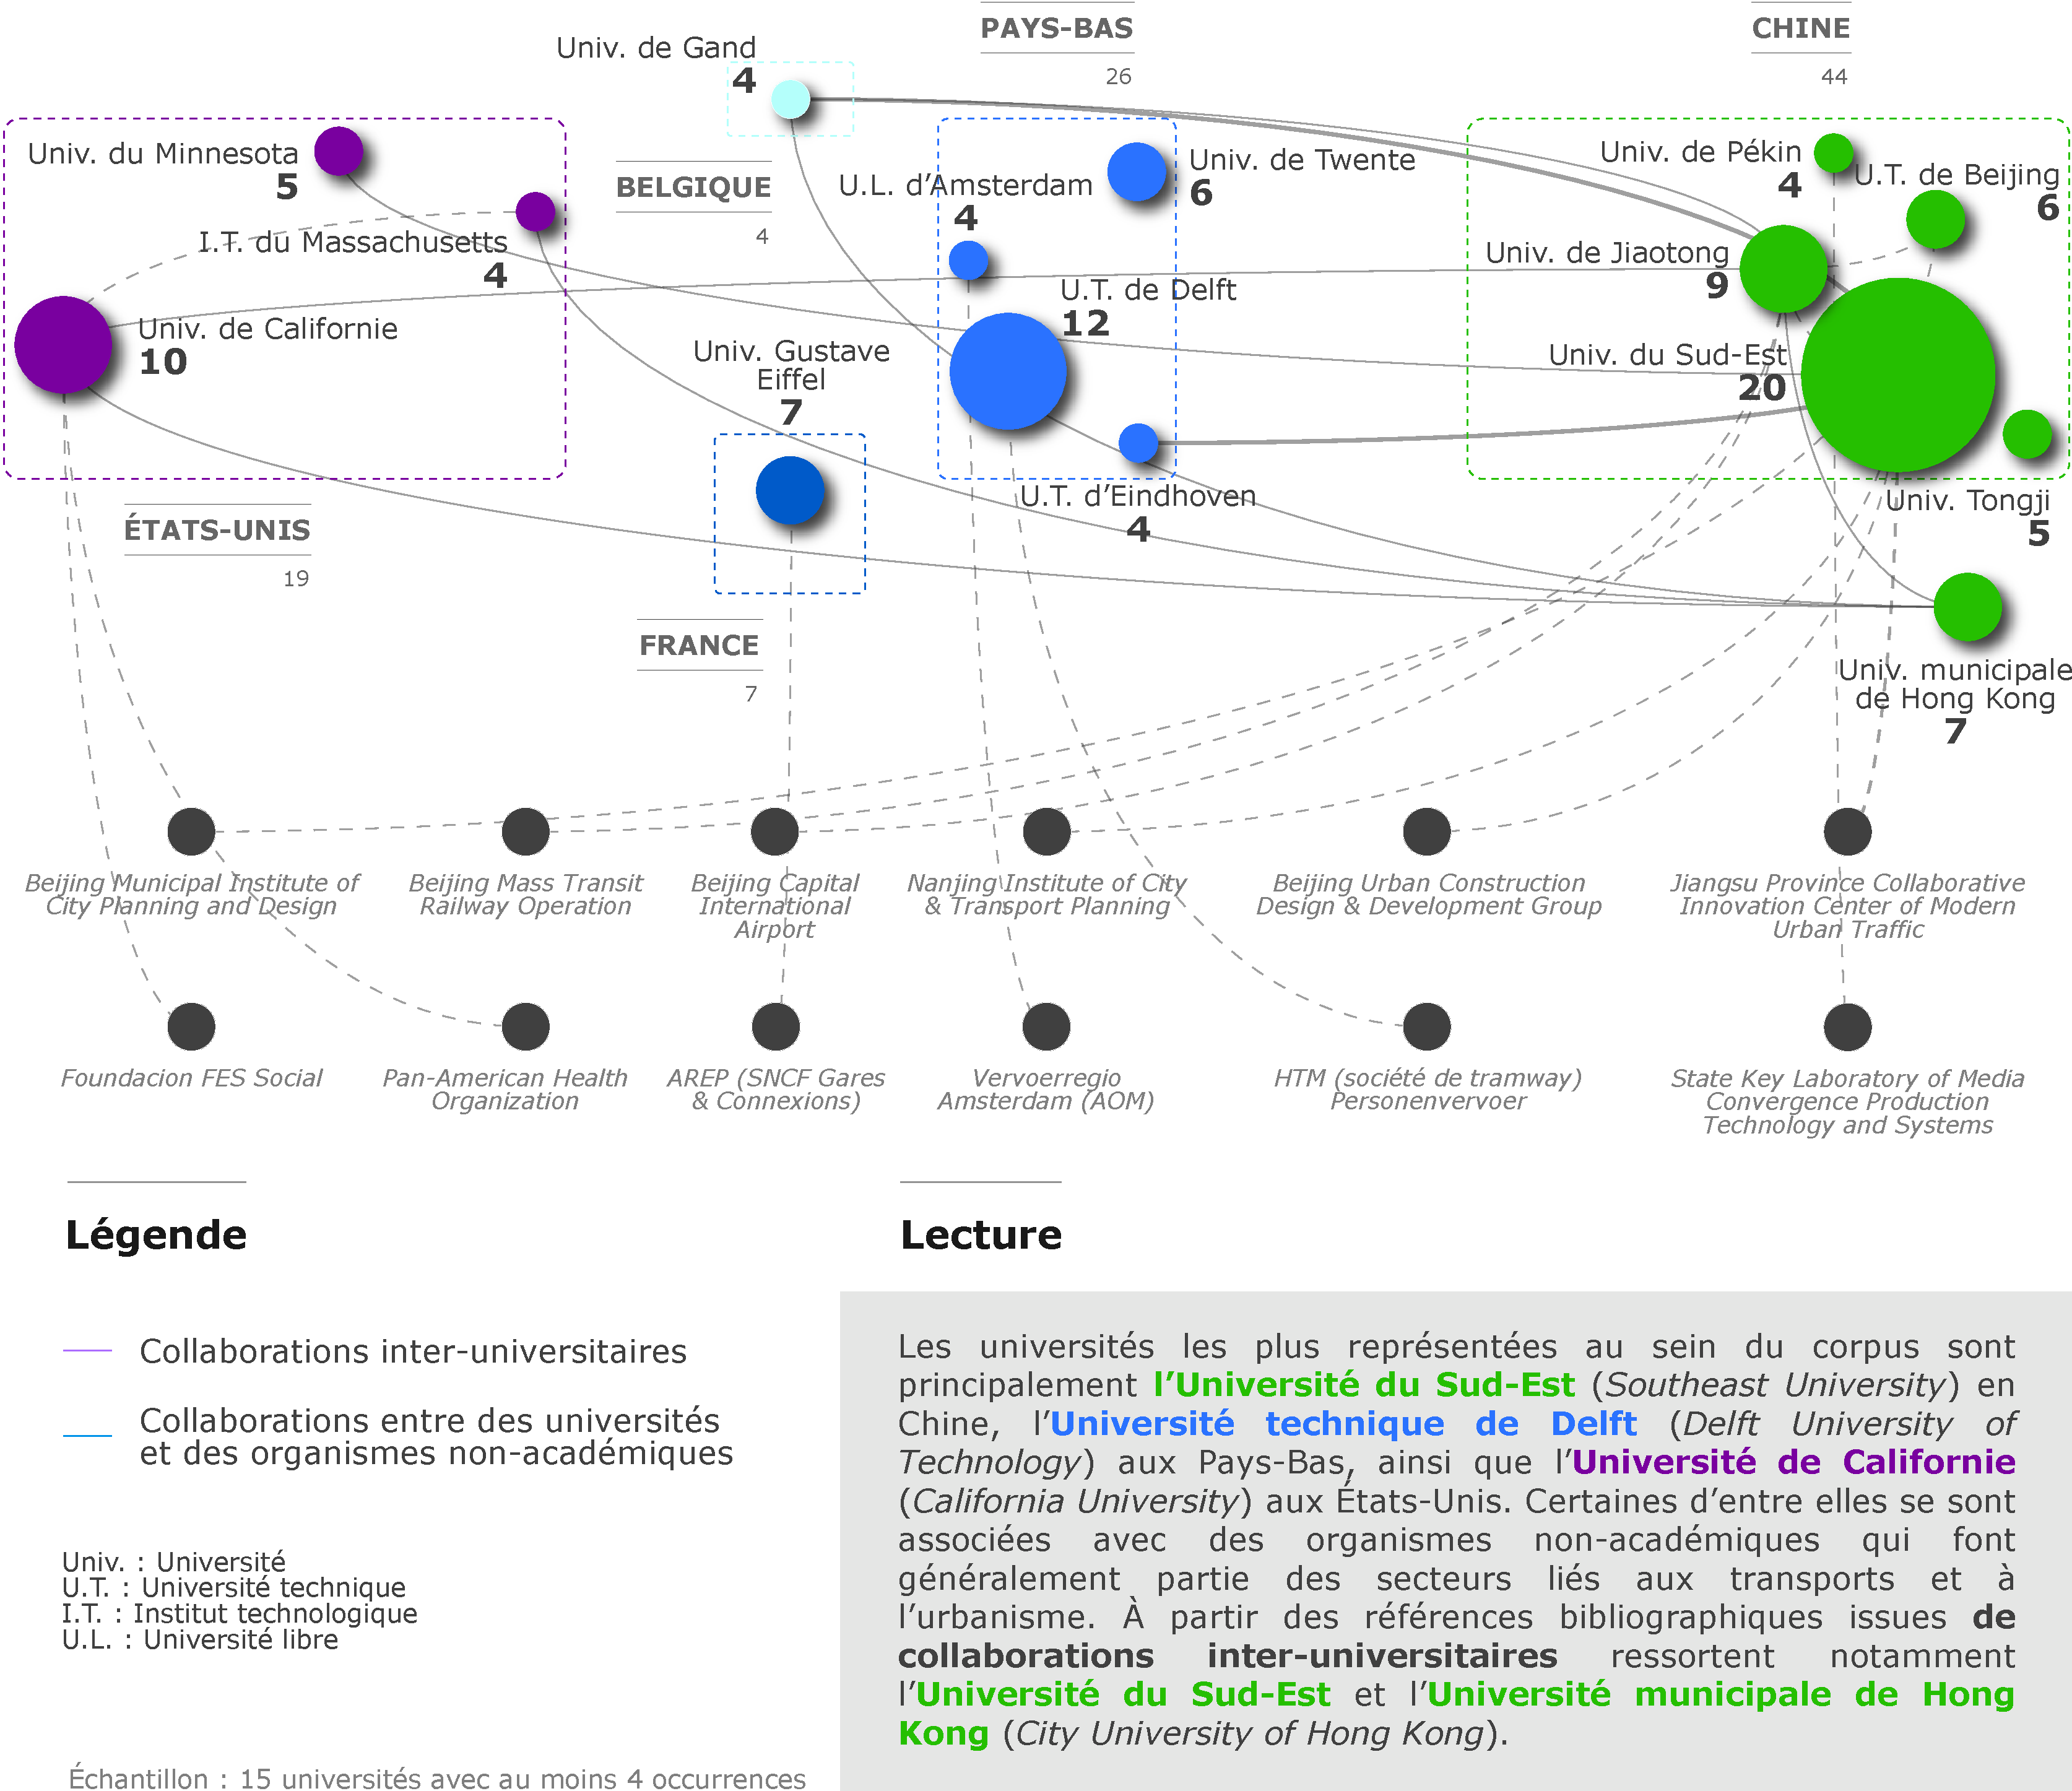
\includegraphics[width=1\columnwidth]{src/Figures/Chap-2/FR_RSL_Collaborations_universites.pdf}}
        \vspace{5pt}
        \begin{flushright}\scriptsize{
        Auteur~: \textcolor{blue}{Dylan Moinse (2023)}
        %\\
        %Réalisation avec \Marque{Excel}~et sur \Marque{Illustrator}
        }\end{flushright}
    \end{figure}

    % Universités et institutions
Du point de vue des institutions représentées dans les 238 contributions scientifiques incorporées au sein de la \acrshort{RSL}, se présente un total de 268 universités, instituts, organismes et entreprises publiques ou privées uniques. Les quinze institutions les plus récurrentes représentent à elles seules plus d'un quart de la distribution (429 valeurs observées). Comme figurées dans l'\hyperref[fig-chap2:copublications-universites-rsl]{illustration~\ref{fig-chap2:copublications-universites-rsl}} (page~\pageref{fig-chap2:copublications-universites-rsl}), les principales universités identifiées dans la documentation sont l'Université du Sud-Est à Nanjing (20), suivie par l'Université de technologie de Delft (12), l'Université de Californie à Berkeley (10), l'Université Jiaotong de Beijing (9), l'Université municipale d'Hong~Kong (7), l'Université Gustave Eiffel en France (7), l'Université de technologie de Beijing (6), l'Université de Twente à Enschede (6), l'Université de Tongji à Shanghai (5), l'Université du Minnesota Twin Cities à Minneapolis et Saint-Paul (5), la Vrije Universiteit d'Amsterdam (4), l'Université technique d'Eindhoven (4), l'Université de Gand (4), l'Institut de technologie du Massachusetts à Cambridge (4) et enfin l'Université de Pékin (4).%%Rédigé%%

    % Collaborations universités et institutions
En interrogeant les collaborations scientifiques à l'échelle universitaire, il s'avère que 128 ouvrages scientifiques se signalent par l'entrecroisement d'au moins deux établissements universitaires ou instituts de recherche au sein d'une même publication. Ainsi, plus de la moitié des contributions scientifiques répertoriées sont marquées par une co-publication pluriversitaire, régulièrement à cheval sur des continents distincts. Les liens prééminents observés se concentrent entre la Chine, les États-Unis, la France, les Pays-Bas et la Belgique. Parmi les partenariats qui ont donné lieu à de telles publications, citons les travaux communs de l'Université du Sud-Est et avec l'Université technique d'Eindhoven \textcolor{blue}{\autocite[]{gan_associations_2021, liu_use_2020, liu_understanding_2020}}\index{Gan, Zuoxian|pagebf}\index{Yang, Min|pagebf}\index{Zeng, Qingcheng|pagebf}\index{Timmermans, Harry~J.~P.|pagebf}\index{Liu, Yang|pagebf}\index{Feng, Tao|pagebf}\index{Ji, Yanjie|pagebf}\index{Shi, Zhuangbin|pagebf}\index{Ji, Yanjie|pagebf}\index{Feng, Tao|pagebf}\index{Timmermans, Harry~J.~P.|pagebf} et avec l'Université de Gand \textcolor{blue}{\autocite[]{chen_what_2022, cheng_comparison_2023, cheng_exploring_2022}}\index{Chen, Wendong|pagebf}\index{Chen, Xuewu|pagebf}\index{Chen, Jingxu|pagebf}\index{Cheng, Long|pagebf}\index{Huang, Jie|pagebf}\index{Jin, Tanhua|pagebf}\index{Chen, Wendong|pagebf}\index{Li, Aoyong|pagebf}\index{Witlox, Frank|pagebf}\index{Cheng, Long|pagebf}\index{Wang, Kailai|pagebf}\index{Vos, Jonas de|pagebf}\index{Huang, Jie|pagebf}\index{Witlox, Frank|pagebf}, tout comme ceux de l'Université municipale d'Hong~Kong avec l'Université de Californie \textcolor{blue}{\autocite{wu_optimal_2020}}\index{Wu, Liyu|pagebf}\index{Gu, Weihua|pagebf}\index{Fan, Wenbo|pagebf}\index{Cassidy, Michael~J.|pagebf} et l'Institut de technologie du Massachusetts \textcolor{blue}{\autocite{cao_e-scooter_2021}}\index{Cao, Zhejing|pagebf}\index{Zhang, Xiaohu|pagebf}\index{Chua, Kelman|pagebf}\index{Yu, Honghai|pagebf}\index{Zhao, Jinhua|pagebf}. Des intervenants opérationnels sont également présents au sein des recherches sur le \acrshort{M-TOD}, essentiellement dans le secteur de la gestion des transports, avec des publications conjointes entre l'Université de Jiaotong et la société d'exploitation des transports en commun \textsl{Beijing Mass Transit Railway Operation Corporation Limited} \textcolor{blue}{\autocite{wang_interchange_2016}}\index{Wang, Zi-jia|pagebf}\index{Chen, Feng|pagebf}\index{Xu, Tian-kun|pagebf} et l'aéroport international \textsl{Beijing Capital International Airport} \textcolor{blue}{\autocite{fan_how_2019}}\index{Fan, Aihua|pagebf}\index{Chen, Xumei|pagebf}\index{Wan, Tao|pagebf}. Pareillement, l'Université du Sud-Est tisse des liens avec les acteurs urbains tels que la \textsl{Nanjing Institute of City \& Transport Planning Co.} \textcolor{blue}{\autocite{zhong_layout_2021}}\index{Zhong, Hongming|pagebf}\index{Liu, Zijian|pagebf}\index{Chen, Jun|pagebf}\index{Hao, Jun|pagebf}\index{Wang, Wei|pagebf} et la \textsl{Beijing Urban Construction Design \& Development Group Co., Limited} \textcolor{blue}{\autocite{yang_empirical_2016}}\index{Yang, Min|pagebf}\index{Liu, Xinlu|pagebf}\index{Wang, Wei|pagebf}\index{Li, Zhibin|pagebf}\index{Zhao, Jingyao|pagebf}. Par ailleurs, des connexions se profilent entre l'Université de Californie et l'organisation à but non lucratif \acrfull{FES} et l'organisation de santé publique \textsl{Pan American Health Organization} \textcolor{blue}{\autocite{cervero_influences_2009}}\index{Cervero, Robert|pagebf}\index{Sarmiento, Olga~L.|pagebf}\index{Jacoby, Enrique|pagebf}\index{Gomez, Luis Fernando|pagebf}\index{Neiman, Andrea|pagebf}.%%Rédigé%%

    % Transition
L'analyse bibliométrique du corpus académique a mis l'accent sur un vaste ensemble documentaire, principalement constitué d'articles scientifiques, parus au sein de revues soumises à une évaluation par les pairs et diffusés en anglais. La grille d'analyse de la \acrshort{RSL}, basée dans cette première sous-partie sur les contours de la recherche en lien avec le \acrshort{M-TOD}, s'est trouvée en mesure d'apporter un aperçu sur les figures, les établissements universitaires et les journaux scientifiques les plus influents autour de cet objet d'étude. Dans la sous-section suivante, nous proposons d'explorer l'état actuel de la littérature scientifique consacrée au \acrshort{TOD} revisité par la mobilité individuelle légère en conduisant une analyse textuelle des contributions scientifiques.

    % 2.2.1.2. Keywords, Content/Body of the Text
    \needspace{1\baselineskip} % Réserve de l'espace
\subsubsection*{Analyse textuelle des productions académiques
    \label{chap2:analyse-textuelle}
    }
    
    % Introduction
L'investigation des métadonnées extraites du corpus académique s'appuie, dans un deuxième temps, sur les systèmes lexicaux employés au sein des ouvrages de recherche. Cette partie de la \acrshort{RSL} intrinsèquement liée à l'analyse textuelle des productions académiques sur le \acrshort{M-TOD} a pour dessein l'identification des pratiques de recherche se matérialisant au travers du vocabulaire utilisé. Originellement, l'étude a été différenciée selon la langue de diffusion, une première catégorie liée à l'usage de l'anglais et se composant de 228 documents et une seconde se déployant en français et constituée de 10~travaux. Toutefois, en raison de la faible représentativité des ouvrages francophones, l'analyse textuelle concentre son attention de manière exclusive sur les publications rédigées en anglais.%%Rédigé%%

    % Analyse des mots-clés~: échantillon et méthodologie
D'un point de vue symbolique, l'examen textuel s'est dirigé vers le contenant des recherches intégrées à la \acrshort{RSL} en interrogeant l'architecture sémantique des productions écrites, construite sur la sélection de mots-clés qui apparaissent généralement à la suite du titre et du résumé. L'agrégation des contributions universitaires a donné lieu à la compilation de 1~336 mots-clés issus de 208 ouvrages, dont 201 en anglais. L'exploration des listes de mots-clés définies par les chercheur·se·s investi·e·s sur le \acrshort{M-TOD} révèle une fréquence moyenne de 6,7 mots-clés par document, revenant à considérer plus de 303 termes distincts, parmi lesquels 260~sont en anglais. Dans la perspective de conduire une analyse comparative des mots-clés mentionnés dans le corpus, une phase préliminaire de nettoyage des données a été entreprise. Ce processus d'harmonisation terminologique a consisté à homogénéiser les ensembles de mots-clés partageant une filiation commune ou une signification affinitaire\footnote{
    À titre d'illustration, nous pouvons évoquer l'agrégation des mots \Guillemets{bicyclette}~et \Guillemets{vélo}~en langue française, ou les expressions \Guillemets{\textsl{transit}}~et \Guillemets{\textsl{public transport}}, ou encore \Guillemets{\textsl{subway}}~et \Guillemets{\textsl{metro}}~en langue anglaise. Bien que cette étape soit cruciale en vue de faciliter la pertinence des données textuelles mobilisées, il convient de signaler les présupposés inhérents à ce travail d'appréciation.
}.%%Rédigé%%

    % Mots-clés~: résultat 1
Par l'entrecroisement des 1~281~mots-clés en anglais, l'analyse textuelle de la présente \acrshort{RSL} met en évidence onze aspects thématiques qui se distinguent au sein des étiquettes lexicales extraites. Pour mener cette analyse lexicale, nous avons établi au préalable plusieurs catégories thématiques. Chaque mot a été classé de manière arbitraire selon la catégorie correspondante à son contexte d'utilisation. Une mise en relief graphique de l'\hyperref[fig-chap2:nuage-mots-cles-rsl]{illustration~\ref{fig-chap2:nuage-mots-cles-rsl}} (page~\pageref{fig-chap2:nuage-mots-cles-rsl}) laisse apparaître les groupements de mots-clés, au sein desquels les thématiques liées à la mobilité individuelle et collective occupent une place hégémonique. Ainsi, les concepts relatifs aux \Guillemets{modes de déplacement individuels}~(282~occurrences), à l’\Guillemets{intermodalité}~(224 occurrences), aux \Guillemets{transports en commun}~(202~occurrences) et à la \Guillemets{mobilité}~(181~occurrences) représentent les principales catégories du classement, en adéquation avec la configuration de l'expression utilisée pour la recherche bibliographique des \Guillemets{Corpus EN et FR}, qui a expressément conduit à l'émergence de ces thématiques (pour rappel, voir le \hyperref[table-chap2:expression-recherche-rsl]{tableau~\ref{table-chap2:expression-recherche-rsl}}, page~\pageref{table-chap2:expression-recherche-rsl}).%%Rédigé%%

    % Figure Nuage de mots-clés RSL
    \begin{figure}[h!]\vspace*{4pt}
        \caption{Nuages de mots-clés anglais extraits de la revue systématique de la littérature et classés par thématique.}
        \label{fig-chap2:nuage-mots-cles-rsl}
        \centerline{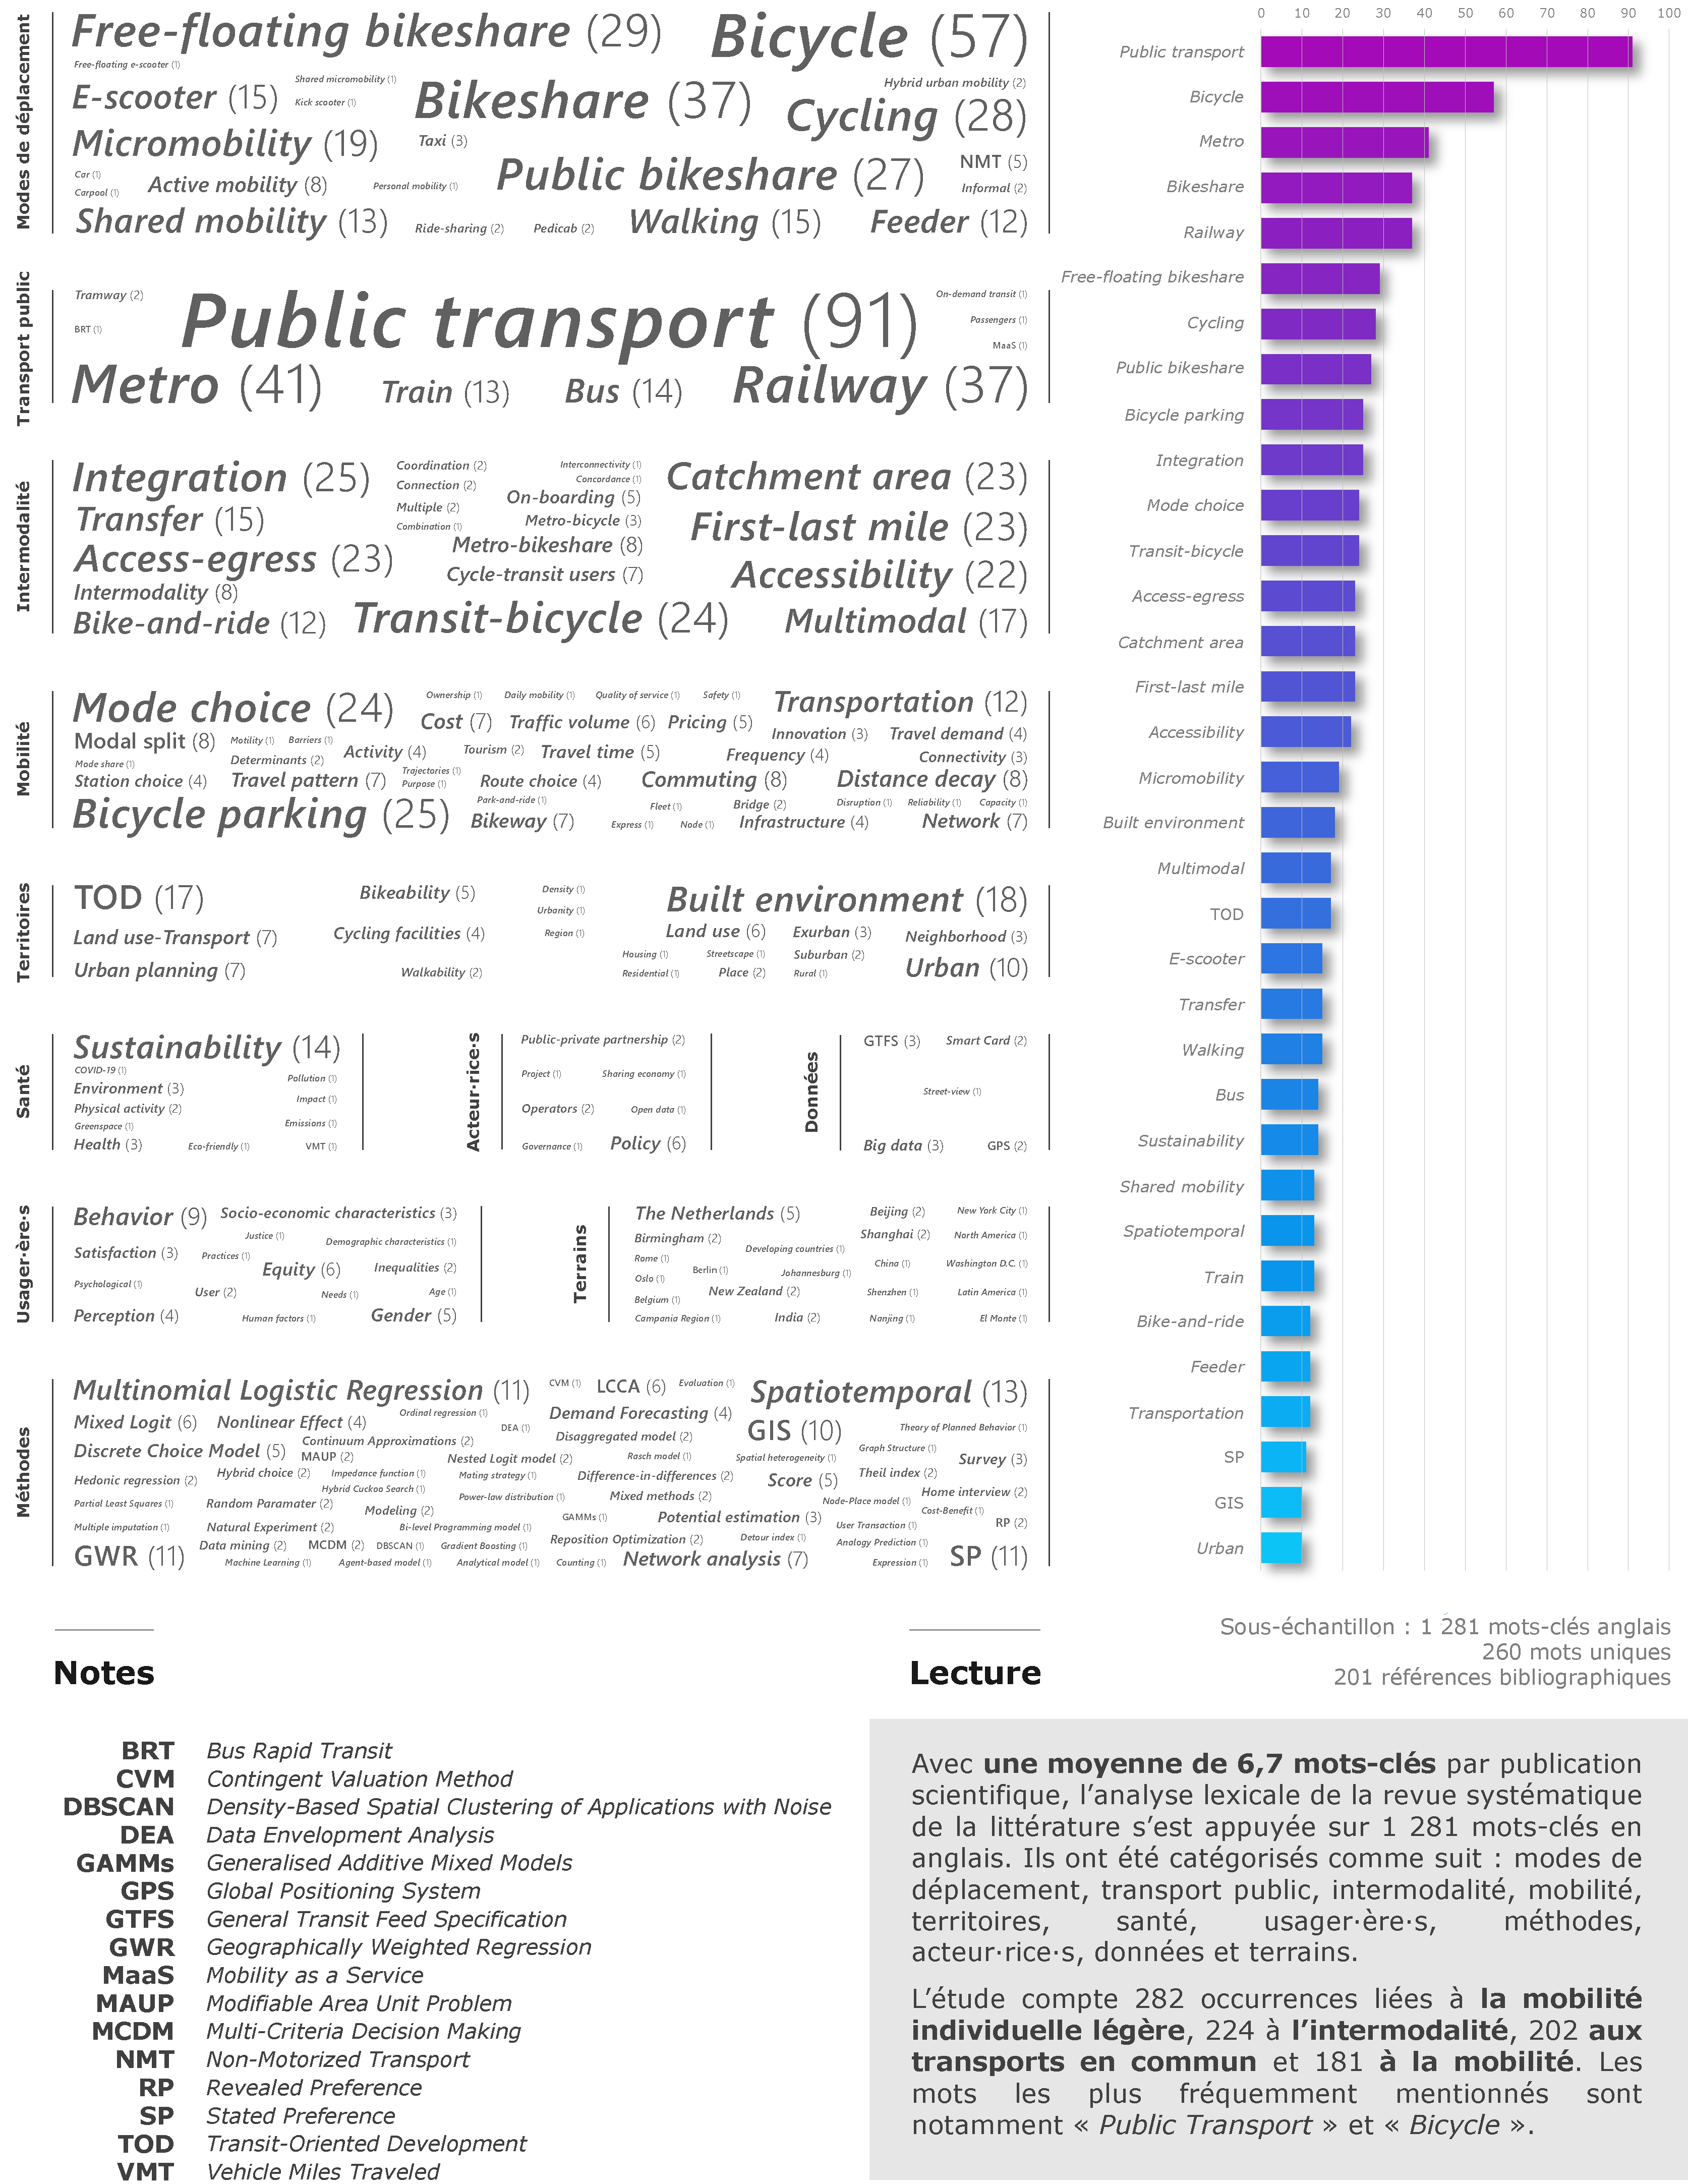
\includegraphics[width=1\columnwidth]{src/Figures/Chap-2/FR_RSL_Nuage_mots_cles_thematiques.pdf}}
        \vspace{5pt}
        \begin{flushright}\scriptsize{
        Auteur~: \textcolor{blue}{Dylan Moinse (2023)}
        %\\
        %Réalisation avec \Marque{Python}~et sur \Marque{Illustrator}
        }\end{flushright}
    \end{figure}

    % Mots-clés~: résultat 2
À l'échelle des mots-clés, c'est principalement dans le registre des \Guillemets{transports en commun}~et du \Guillemets{vélo}~que se manifestent des occurrences prééminentes, comptabilisant respectivement 91 et 57 itérations de termes qui leur sont rattachées. Néanmoins, cette prédominance des mots-clés voile une distribution inégalitaire au sein de chaque thématique mise en observation. Alors que la fréquence des mots-clés se rapportant à \Guillemets{transports en commun}, \Guillemets{modes de déplacement individuels}~et \Guillemets{intermodalité}~est conséquente, s'élevant à 20, 12 et 11~récurrences pour chaque terme en moyenne, cette intensité s'amenuise à 5,5 et 2~répétitions en ce qui concerne les catégories afférentes à \Guillemets{mobilité}, \Guillemets{urbanisme}~et \Guillemets{méthodes}. Ce constat témoigne d'une plus vaste variété de mots-clés dans ces dernières thématiques, parallèlement à un processus d'homogénéisation terminologique perceptible au sein des domaines des modes de déplacement personnels, des transports en commun et de l'intermodalité.%%Rédigé%%

    % Mots-clés~: résultat 3
La manipulation des mots-clés sous l'angle des modes de déplacement et des infrastructures de transport comme objets, tels que \Guillemets{\textsl{bicycle}}~(mentionné à 57 reprises), \Guillemets{\textsl{free-floating bikeshare}}~(29 occurrences), \Guillemets{\textsl{public bikeshare}}~(27 occurrences), \Guillemets{\textsl{metro}}~(41~occurrences), \Guillemets{\textsl{railway}}~(37 occurrences) ou encore \Guillemets{\textsl{bicycle parking}}~(25 occurrences), reflète une intrication qui se cristallise en signaux lexicaux, perpétuant le schéma conventionnel du domaine du transport (voir l'\hyperref[fig-chap2:nuage-mots-cles-rsl]{illustration~\ref{fig-chap2:nuage-mots-cles-rsl}}, page~\pageref{fig-chap2:nuage-mots-cles-rsl}). De manière analogue à cette démarche ancrée dans le paradigme des transports, se profile un vaste domaine sémantique dévolu au \Guillemets{tournant de la mobilité}~\textcolor{blue}{\autocites{sheller_new_2006}[8]{sheller_mobilizing_2016}[13]{randell_no_2020}}\index{Sheller, Mimi|pagebf}\index{Urry, John|pagebf}\index{Randell, Richard|pagebf}, marqué par l'utilisation d'expressions à l'image d'\Guillemets{\textsl{accessibility}}~(22~occurrences), \Guillemets{\textsl{sustainability}}~(14 occurrences), \Guillemets{\textsl{behavior}}~(9 occurrences), \Guillemets{\textsl{policy}}~(6 occurrences), \Guillemets{\textsl{equity}}~(6 occurrences) ou encore \Guillemets{\textsl{bikeability}}~(5 occurrences). Certes, dans une moindre mesure, nous pouvons discerner l'implication de l'urbanisme et notamment de son articulation avec la mobilité, comme en témoignent le concept de \Guillemets{\textsl{TOD}}~(17 occurrences) ou \Guillemets{\textsl{land use-transport}}~(7 occurrences).%%Rédigé%%

    % Mots-clés~: résultat 4
En sondant les interactions entre les mots-clés précités, il est intéressant de relever les liaisons étroites qui associent certaines catégories entre elles. La majorité des listes de vocables tend à établir des passerelles interconnectant les catégories relatives aux \Guillemets{transports en commun}~et aux \Guillemets{modes de déplacement individuels}. Parmi les 201~références anglophones, 155 d'entre elles tissent un dialogue entre ces deux thématiques, qui s'exprime par le choix délibéré d'une liste de mots-clés rattachés à la mobilité collective et personnelle. De surcroît, 59 publications scientifiques se distinguent par une configuration spécifique, prenant la forme d'une suite lexicale ordonnée de la façon suivante~: le premier mot-clé de la liste se réfère aux \Guillemets{transports en commun}, suivi des \Guillemets{modes de déplacement individuels}~et d'un troisième terme invoquant l'\Guillemets{intermodalité}.%%Rédigé%%

    % Figure Mots contenu RSL
    \begin{figure}[h!]\vspace*{4pt}
        \caption{Nuage de mots tirés du contenu intégral des travaux académiques anglophones intégrés dans la revue systématique de la littérature.}
        \label{fig-chap2:contenu-textuel-rsl}
        \centerline{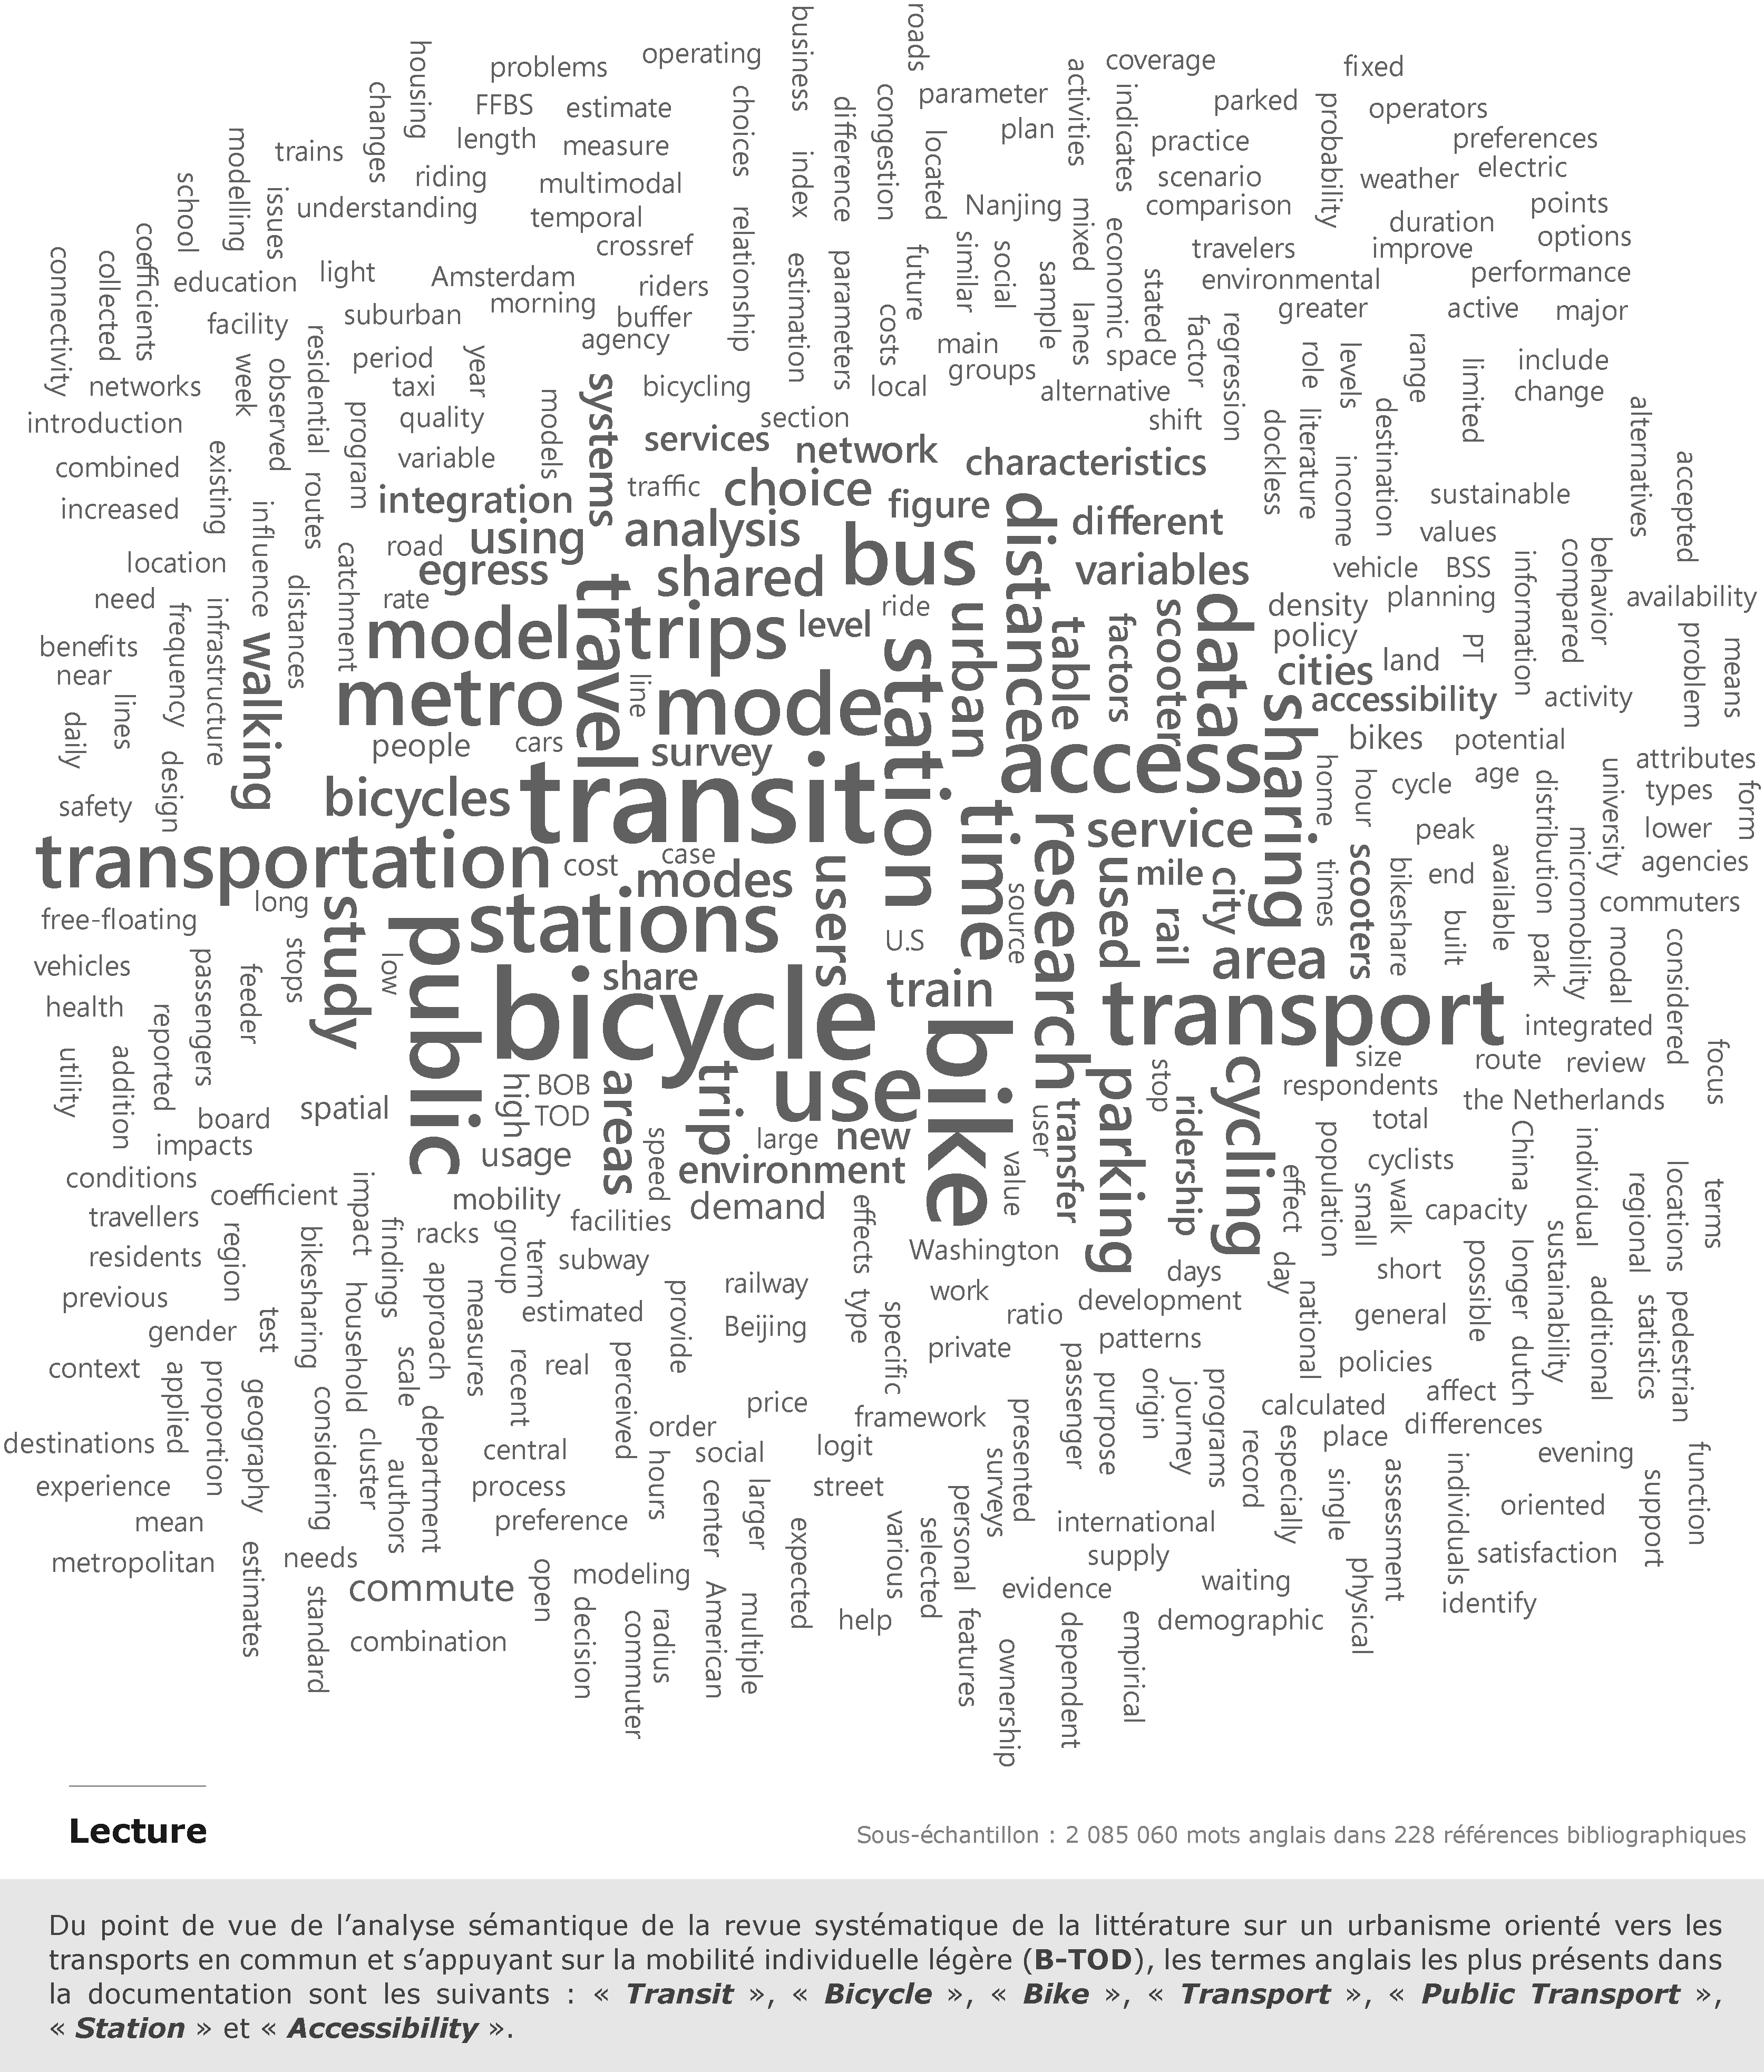
\includegraphics[width=1\columnwidth]{src/Figures/Chap-2/FR_RSL_Mots_contenu.pdf}}
        \vspace{5pt}
        \begin{flushright}\scriptsize{
        Auteur~: \textcolor{blue}{Dylan Moinse (2023)}
        %\\
        %Réalisation avec \Marque{Python}~et sur \Marque{Illustrator}
        }\end{flushright}
    \end{figure}
    
    % Contenu mots RSL
L'exploitation textuelle a été approfondie au travers d'une analyse du contenu intégral de chaque publication scientifique rapportée en langue anglaise. Comme en témoigne l'\hyperref[fig-chap2:contenu-textuel-rsl]{illustration~\ref{fig-chap2:contenu-textuel-rsl}} (page~\pageref{fig-chap2:contenu-textuel-rsl}), l'examen des cent termes les plus récurrents au sein des documents\footnote{
    Afin de procéder à la classification des champs lexicaux identifiés dans les documents analysés, nous avons procédé à une étape de nettoyage des termes ayant trait à la vie quotidienne ou à la recherche scientifique de manière générale, dans la langue anglaise. Ces expressions courantes ont ultérieurement été exclues de l'analyse, à l'instar de \Guillemets{\textsl{the}}, \Guillemets{\textsl{a}}, \Guillemets{\textsl{and}}, \Guillemets{\textsl{we}}, \Guillemets{\textsl{for}}, \Guillemets{\textsl{study}}, \Guillemets{\textsl{scientific}}, \Guillemets{\textsl{methods}}~ou encore \Guillemets{\textsl{results}}.
} renforce la tendance préalablement identifiée au niveau des mots-clés, se traduisant principalement par la prépondérance des termes \Guillemets{\textsl{transit}}, \Guillemets{\textsl{bicycle}}, \Guillemets{\textsl{bike}}, \Guillemets{\textsl{transport}}, \Guillemets{\textsl{public transport}}, \Guillemets{\textsl{station}}~et \Guillemets{\textsl{accessibility}}. Néanmoins, il faut souligner l'influence substantielle de certains mots, tels que \Guillemets{\textsl{use}}, \Guillemets{\textsl{access}}, \Guillemets{\textsl{distance}}, \Guillemets{\textsl{area}}, \Guillemets{\textsl{users}}~ou \Guillemets{\textsl{service}}, qui revêtent une dimension liée aux usages, usager·ère·s et aux distances-temps parcourues. En revanche, il est à noter que la présence lexicale en lien avec l'urbanisme demeure pratiquement absente dans les écrits, à l'exception de quelques occurrences événementielles, comme \Guillemets{\textsl{density}}, \Guillemets{\textsl{mixed}}, \Guillemets{\textsl{TOD}}~ou \Guillemets{\textsl{land}}.%%Rédigé%%

    % Transition
À la lecture des termes scrutés au sein du corpus de la \acrshort{RSL}, résultent en premier plan les divers modes de transports collectifs et individuels inscrits au cœur d'un développement urbain orienté vers les transports en commun et s'appuyant sur la mobilité individuelle légère. En considération de la rapide évolution de la pratique de mobilité, des techniques et des technologies propres à ces différents objets de déplacement, la sous-section suivante s'emploie à mettre en perspective les travaux de recherche en lien avec le \acrshort{M-TOD}, en mettant l'accent sur l'évolution des champs d'investigation émergents.%%Rédigé%%

    % 2.2.1.3. micro-mobilité, TC
    \needspace{1\baselineskip} % Réserve de l'espace
\subsubsection*{Évolution des recherches sur la synergie entre les transports en commun et la mobilité individuelle légère
    \label{chap2:evolution-recherches-tc-mobilite-individuelle-legere}
    }
    
    % Tendance depuis 1993
L'analyse de la répartition temporelle des publications scientifiques intégrées à la \acrshort{RSL} offre une perspective globale sur les caractéristiques et les avancées qui délimitent ce corpus de littérature. La trajectoire chronologique du corpus bibliographique consacré à l'intégration de la mobilité individuelle légère aux réseaux de transports en commun dépeint une croissance continue entre~1993~et~2021. À partir de~2015, le seuil annuel de dix publications scientifiques a été systématiquement dépassé, suggérant un intérêt croissant de la recherche autour de ce sujet. En l'espace de seulement quatre années consécutives, le nombre de documents académiques recensés a doublé, avec l'apparition de 129 nouveaux travaux partagés entre~2019 et le début de l'année 2023.%%Rédigé%%

    % Objectif
Conformément au protocole méthodologique défini dans la présente \acrshort{RSL}, la date minimale retenue pour cette étude bibliométrique a été fixée à 1993, en référence à la conceptualisation du \acrshort{TOD} par \textcolor{blue}{Peter} \textcolor{blue}{\textcite{calthorpe_next_1993}}\index{Calthorpe, Peter|pagebf}. L'étude bibliographique ainsi exposée vise à dévoiler les caractéristiques de ce corpus élaboré sur trois décennies de recherches internationales. Cependant, il est primordial de reconnaître l'existence d'œuvres antérieures traitant du sujet à l'étude. Bien que la croissance observée des publications scientifiques englobe des travaux en anglais et en français, l'émergence d'œuvres francophones se produit à un stade ultérieur, à partir de 2015. Néanmoins, ce sous-ensemble demeure de taille restreinte pour établir des conclusions définitives. En revanche, la littérature scientifique se déployant dans des contextes européens se développe précocement dès l'année 2000.%%Rédigé%%

    % Figure chronologie RSL modes de transport
    \begin{figure}[h!]\vspace*{4pt}
        \caption{Évolution des publications scientifiques sur la combinaison entre les transports en commun et la mobilité individuelle légère, au sein de la revue systématique de la littérature.}
        \label{fig-chap2:chronologie-modes-deplacements-rsl}
        \centerline{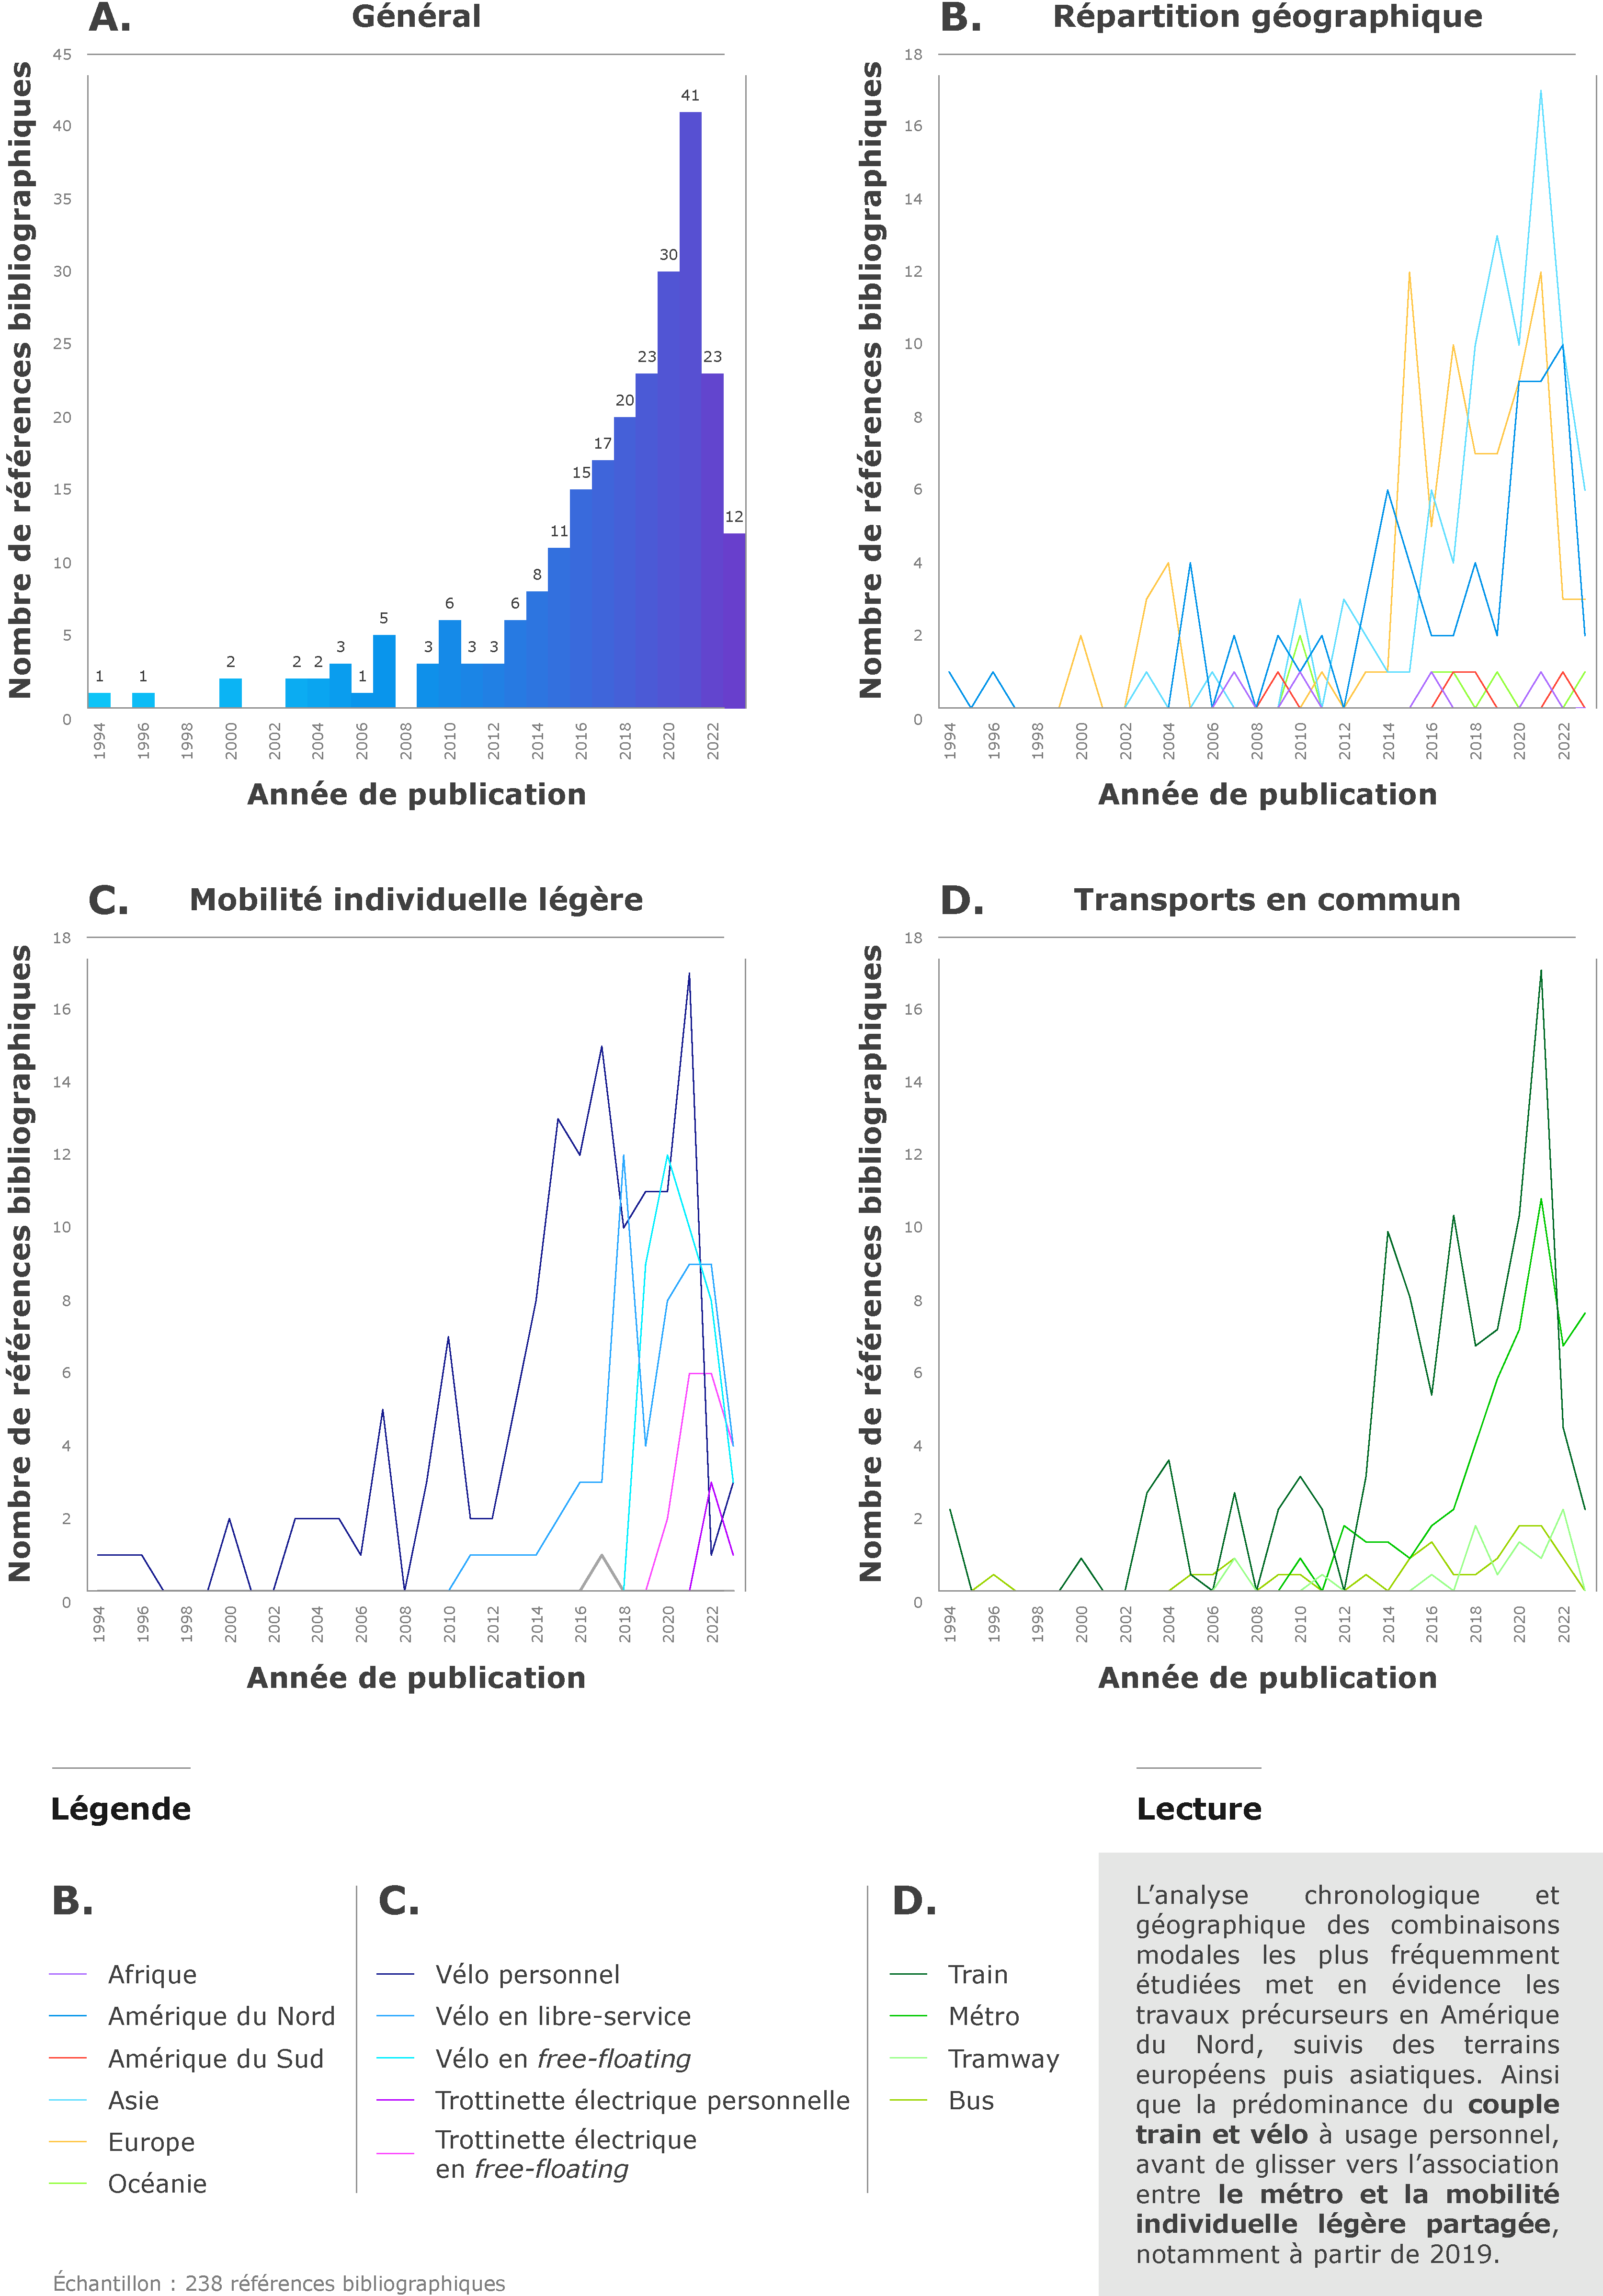
\includegraphics[width=1\columnwidth]{src/Figures/Chap-2/FR_RSL_Chronologie.pdf}}
        \vspace{5pt}
        \begin{flushright}\scriptsize{
        Auteur~: \textcolor{blue}{Dylan Moinse (2023)}
        %\\
        %Réalisation avec \Marque{Excel}, \Marque{Python}~et sur \Marque{Illustrator}
        }\end{flushright}
    \end{figure}

    % Chronologie par micro-mobilités
L'approche chronologique du \acrshort{M-TOD}, telle qu'elle se dessine dans la littérature scientifique, offre des perspectives éclairantes sur l'essor de la mobilité individuelle légère (voir l'\hyperref[annexes:rsl-combinaisons-modales]{annexe~\ref{annexes:rsl-combinaisons-modales}}, page~\pageref{annexes:rsl-combinaisons-modales}) et son apport potentiel sur le développement du modèle urbain. L'\hyperref[fig-chap2:chronologie-modes-deplacements-rsl]{illustration~\ref{fig-chap2:chronologie-modes-deplacements-rsl}} (page~\pageref{fig-chap2:chronologie-modes-deplacements-rsl}) révèle la place éminente qu'a occupée le vélo conventionnel dans la recherche internationale de 1994 à 2017, représentant 89~\% des publications au cours de cette période. Cependant, cette position dominante a progressivement été remise en question, avec une présence du vélo traditionnel dans seulement 41~\% des études entre~2018~et~2021, et dans à peine 4~\% des publications les plus récentes. Cette dynamique défavorable a tout d'abord profité à l'exploration des systèmes de partage de \acrfull{VLS}, dont l'intérêt s'est accru à partir de 2011. Par la suite, à partir de 2019, l'attention s'est déplacée vers les systèmes de partage de \acrfull{VFF}. Plus récemment, le corpus de recherche a manifesté un intérêt croissant pour les systèmes de partage de \acrfull{TEFF}. Toutefois, la \acrfull{TEP} reste absente des enquêtes, soulignant un contraste apparent entre l'effervescence récente des études sur les services partagés et la paucité de recherches sur l'utilisation privée de la trottinette électrique. Cette observation est à resituer dans le contexte de l'essor du vélo et de la micro-mobilité partagés, comme en témoigne l'analyse descriptive réalisée par \textcolor{blue}{\textcite[298]{zhang_built_2023}}\index{Zhang, Yushan|pagebf}\index{Kasraian, Dena|pagebf}\index{Wesemael, Pieter van|pagebf} au sein de sa \acrshort{RSL}, qui démontre que les trois quarts de la documentation à ce sujet sont apparus entre~2019~et~2022.%%Rédigé%%

    % Chronologie par transports en commun
L'étude séquentielle des systèmes de transports en commun examinés au sein de la littérature scientifique jette également une lumière sur les tendances générales qui se sont dessinées au cours des trois décennies enquêtées. Telle que l'indique l'\hyperref[fig-chap2:chronologie-modes-deplacements-rsl]{illustration~\ref{fig-chap2:chronologie-modes-deplacements-rsl}} (page~\pageref{fig-chap2:chronologie-modes-deplacements-rsl}), les recherches internationales portant sur le \acrshort{M-TOD} ont manifesté un intérêt particulier pour les modes ferroviaires interurbains de 1994 à 2017, avec une attention particulière portée au \acrfull{TER}, en conjonction avec le vélo conventionnel. En contraste, le système de métro, qui était jusqu'alors relativement en retrait jusqu'en 2012, a connu un renouveau d'intérêt à partir de 2019, coïncidant avec l'augmentation de l'attention portée aux systèmes de \acrshort{VFF} et de \acrshort{TEFF}. Par ailleurs, il ne faut pas omettre les études sur l'association de la mobilité individuelle légère avec le bus, notamment le \acrfull{BHNS}, ainsi qu'avec le tramway, lesquels maintiennent une présence secondaire, mais constante dans les publications scientifiques. Dans l'ensemble, l'analyse chronologique des combinaisons modales les plus fréquemment étudiées expose un schéma principal~: l'ascendant initial du couple train et vélo personnel dans les travaux académiques sur le \acrshort{M-TOD}, cédant progressivement la place au mariage entre le métro et les services de vélo et de micro-mobilité.%%Rédigé%%

    % Chronologie par micro-mobilités partagées (maturation)
Bien que la littérature scientifique portant sur la mobilité individuelle légère, et notamment sur le vélo et la micro-mobilité partagés, se soit développée ces dernières années, les travaux de recherche s'intéressent à diverses phases de développement de ces services de mobilité sur le territoire enquêté. En interrogeant la différence de période entre le moment où le service de mobilité individuelle légère a été mis en place et le moment où la donnée a été collectée et traitée dans la documentation analysée, nous avons alors exploré les divers stades de maturation étudiés en fonction des modes de déplacement composant le partage de vélos et de trottinettes. Ces services de mobilité sont majoritairement étudiés lors de son récent développement, soit environ trois ans (quarante mois) après sa mise en service sur le territoire \textcolor{blue}{\autocite[298]{zhang_built_2023}}\index{Zhang, Yushan|pagebf}\index{Kasraian, Dena|pagebf}\index{Wesemael, Pieter van|pagebf}. L'écart-type de la distribution observée est cependant important, avec une moyenne d'écart égale à quatre ans, ce qui revient à considérer une proportion importante de travaux de recherche s'intéressant à un stade de développement plus avancé. En effet, cette distribution inégalitaire s'explique notamment par les différences existantes selon le type de mobilité individuelle légère partagée analysé~:
    \begin{customitemize}
        \item Le corpus sur le système de \acrshort{VLS} est le plus diversifié, avec des études s'intéressant principalement à une implantation du service depuis cinq ans. Nous pouvons citer les travaux d'\textcolor{blue}{\textcite{aljeri_impacts_2020, andersson_neighbourhood_2021, ma_estimating_2019, ashraf_impacts_2021, liu_understanding_2020, kuijk_preferences_2022, gu_measuring_2019, kong_deciphering_2020, radzimski_exploring_2021, romm_differences_2022, tarpin-pitre_typology_2020}}\index{Aljeri, Moathe|pagebf}\index{Andersson, David Emanuel|pagebf}\index{Ma, Ting|pagebf}\index{Ashraf, Md Tanvir|pagebf}\index{Liu, Yang|pagebf}\index{Kuijk, Roy~J. van|pagebf}\index{Gu, Tianqi|pagebf}\index{Kong, Hui|pagebf}\index{Radzimski, Adam|pagebf}\index{Dzięcielski, Michał|pagebf}\index{Romm, Daniel|pagebf}\index{Verma, Priyanka|pagebf}\index{Karpinski, Elizabeth|pagebf}\index{Sanders, Tracy~L.|pagebf}\index{McKenzie, Grant|pagebf}\index{Tarpin-Pitre, Léandre|pagebf} qui s'intéressent aux effets produits par le \acrshort{VLS} sur le réseau de transport en commun, à New York City, Taipei, Washington~D.C., Nanjing, Suzhou, Boston et Montréal entre cinq et sept ans après sa mise en service. Tandis que \textcolor{blue}{\textcite{cheng_promoting_2022, cheng_expanding_2018, yen_how_2023, tang_uncovering_2021, bocker_bike_2020}}\index{Cheng, Long|pagebf}\index{Jin, Tanhua|pagebf}\index{Wang, Kailai|pagebf}\index{Lee, Yongsung|pagebf}\index{Witlox, Frank|pagebf}\index{Cheng, Yung-Hsiang|pagebf}\index{Yen,~B.T.H.|pagebf}\index{Mulley, Corinne|pagebf}\index{Yeh, Chia-Jung|pagebf}\index{Tang, Jinjun|pagebf}\index{Böcker, Lars|pagebf} analysent l'impact de l'environnement urbain sur le système de mobilité, à Nanjing, Kaohsiung, Taipei, Shenzhen et Oslo entre huit et quinze ans après~;
        \item Le \acrshort{VFF} est plus généralement étudié deux ans après son implantation sur le territoire, alors que le premier quart de la documentation à ce sujet s'intéresse à ce service moins d'un an après. Ainsi, \textcolor{blue}{\textcite{chen_what_2022, fan_dockless_2020, qiu_interplay_2021, fan_how_2019, jin_competition_2019, li_integration_2020, li_unbalanced_2022, li_factors_2020, liu_use_2020, wu_identification_2023, yang_spatiotemporal_2019}}\index{Chen, Wendong|pagebf}\index{Fan, Yichun|pagebf}\index{Qiu, Waishan|pagebf}\index{Jin, Haitao|pagebf}\index{Jin, Fengjun|pagebf}\index{Wang, Jiao'e|pagebf}\index{Sun, Wei|pagebf}\index{Dong, Libo|pagebf}\index{Li, Jie|pagebf}\index{Li, Lili|pagebf}\index{Li, Xuefeng|pagebf}\index{Liu, Yang|pagebf}\index{Wu, Hao|pagebf}\index{Wang, Yanhui|pagebf}\index{Sun, Yuqing|pagebf}\index{Yin, Duoduo|pagebf}\index{Li, Zhanxing|pagebf}\index{Luo, Xiaoyue|pagebf}\index{Yang, Yuanxuan|pagebf} étudient l'usage du \acrshort{VFF} en combinaison avec le réseau de transport en commun, à Nanjing, Beijing, Ithaca, Suzhou, Shenzhen, Nanjing et Nanchang, un à deux ans après sa mise en place. De la même manière qu'avec le \acrshort{VLS}, \textcolor{blue}{\textcite{cheng_exploring_2022, chu_last_2021, guo_built_2020, guo_role_2021, hu_study_2019}}\index{Cheng, Long|pagebf}\index{Wang, Kailai|pagebf}\index{Vos, Jonas de|pagebf}\index{Huang, Jie|pagebf}\index{Witlox, Frank|pagebf}\index{Chu, Junhong|pagebf}\index{Duan, Yige|pagebf}\index{Yang, Xianling|pagebf}\index{Wang, Li|pagebf}\index{Guo, Yuanyuan|pagebf}\index{Hu, Li|pagebf}\index{He, Sylvia~Y.|pagebf} se focalisent sur le rôle de l'environnement urbain en lien avec le \acrshort{VFF} en intermodalité, à Nanjing, Beijing et Shenzhen~;
        \item En dernier lieu, la moitié de la littérature sur la \acrshort{TEFF} en association avec les transports en commun adopte un terrain bénéficiant de la micro-mobilité partagée depuis moins d'un an. L'ensemble des productions scientifiques à ce sujet examinent l'usage de la \acrshort{TEFF} en intermodalité, à Séoul, Austin, Rome, Seattle, Oslo, Berlin, New York City, Columbus, Chicago et Nashville \textcolor{blue}{\autocite{baek_electric_2021, zuniga-garcia_evaluation_2022, vinagre_diaz_blind_2023, beale_integrating_2023, fearnley_patterns_2020, heumann_spatiotemporal_2021, lee_forecasting_2021, li_measuring_2022, mohammadian_analyzing_2022, ziedan_complement_2021}}\index{Baek, Kwangho|pagebf}\index{Zuniga-Garcia, Natalia|pagebf}\index{Vinagre Díaz, Juan José|pagebf}\index{Beale, Kirsten|pagebf}\index{Fearnley, Nils|pagebf}\index{Heumann, Maximilian|pagebf}\index{Li, Mina|pagebf}\index{Li, Xia|pagebf}\index{Mohammadian, Abolfazl|pagebf}\index{Ziedan, Abubakr|pagebf}\index{Shah, Nitesh~R.|pagebf}\index{Wen, Yi|pagebf}\index{Brakewood, Candace|pagebf}\index{Cherry, Christopher~R.|pagebf}\index{Cole, Justin|pagebf}.
    \end{customitemize}%%Rédigé%%

    % Discussion maturation
Partant de ce constat, il apparaît clairement que les services de vélopartage et de micromobilité partagée ne jouissent pas tous de la même temporalité entre leur mise en œuvre et leur période d'investigation. Cette analyse statistique met en lumière des implications quant à la préférence pour certaines thématiques de recherche adaptées au contexte temporel. En général, les systèmes de \acrshort{VLS} disposent d'un temps de maturation suffisant pour faire l'objet d'évaluations sur leurs effets sur les systèmes de mobilité et urbains. À l'opposé, les services de \textsl{free-floating}, nettement plus récents, profitent davantage d'études liées aux comportements de mobilité et à leur régulation en milieu urbain, alors que leurs impacts à terme sur les territoires restent nettement moins explorés.%%Rédigé%%

    % Chronologie par terrains géographiques et transition
En approfondissant l'analyse de l'évolution des sujets d'étude, du binôme train et vélo à celui de métro et services de mobilité partagé, il est envisageable d'incorporer une nouvelle variable liée à la géographie des terrains de recherche retenus. Les études de cas de nature européenne se révèlent en abondance lorsqu'une attention conjointe est portée à la dimension temporelle des publications ainsi qu'aux régions géographiques analysées dans le contexte du \acrshort{M-TOD}. De la période allant de~2000~à~2009, les références bibliographiques adossées à un périmètre géographique européen s'établissent comme constitutives de 8 des 18 documents consacrés dans la \acrshort{RSL}, alors que dès l'année 2010, seulement 62~des 218 investigations répertoriées retiennent une aire géographique située au sein du Vieux Continent. En effet, les recherches portant sur les interactions entre les réseaux de transport en commun et la mobilité individuelle légère en Europe se concentrent majoritairement sur les relations existantes ou potentielles entre le \acrshort{TER} et le vélo à usage individuel (voir l'\hyperref[fig-chap2:chronologie-modes-deplacements-rsl]{illustration~\ref{fig-chap2:chronologie-modes-deplacements-rsl}}, page~\pageref{fig-chap2:chronologie-modes-deplacements-rsl}). Cette transition peut être attribuée à l'émergence des terrains asiatiques à partir de 2010 ainsi qu'à la résurgence des investigations nord-américaines à partir de 2013. Dans le cadre de la sous-section qui suit et qui traite de l'état actuel de la littérature scientifique sur un \acrshort{TOD} intégrant la mobilité individuelle légère, nous allons rendre compte de la répartition géographique des publications scientifiques en vue de saisir les contours temporels et spatiaux de ce sujet de recherche.%%Rédigé%%

    % 2.2.1.4. Terrains géographiques
    \needspace{1\baselineskip} % Réserve de l'espace
\subsubsection*{Exploration des terrains géographiques investis
    \label{chap2:exploration-terrains-geographiques}
    }
    
    % Répartition géographique par continent
Examiner les terrains géographiques étudiés dans les productions académiques permet d'apporter une contextualisation aux phénomènes observés, tout en contribuant à une compréhension holistique des problèmes de recherche et en identifiant certaines lacunes. L'approche chronologique adoptée dans l'analyse bibliométrique révèle une prévalence marquée des trois continents antérieurement évoqués, à savoir l'Amérique du Nord, l'Asie et l'Europe. La \Guillemets{Nouvelle Triade}, en tant que triptyque des principaux nœuds d'échange mondialisés, s'octroie une part substantielle des études de cas sélectionnés, à raison de 26,4~\%, 36~\% et 32~\% respectivement pour les trois régions mentionnées. Inversement, l'Afrique, l'Amérique du Sud et l'Océanie affichent, en revanche, une présence marginale dans la base de données, se chiffrant à seulement 6~\% du registre bibliographique (voir la \hyperref[fig-chap2:terrains-geographiques-continents]{carte~\ref{fig-chap2:terrains-geographiques-continents}}, page~\pageref{fig-chap2:terrains-geographiques-continents}). Sur les 59 articles scientifiques traitant du vélo et de la micro-mobilité à travers la \acrshort{RSL} publiée par \textcolor{blue}{\textcite[298]{zhang_built_2023}}\index{Zhang, Yushan|pagebf}\index{Kasraian, Dena|pagebf}\index{Wesemael, Pieter van|pagebf}, 48 d'entre eux examinent ainsi un terrain en Europe, en Amérique du Nord ou en Asie.%%Rédigé%%

    % Carte terrains géographiques pays
    \begin{carte}[h!]\vspace*{4pt}
        \caption{Cartographie des terrains géographiques explorés dans la revue systématique de la littérature, aggrégés par pays.}
        \label{fig-chap2:terrains-geographiques-continents}
        \centerline{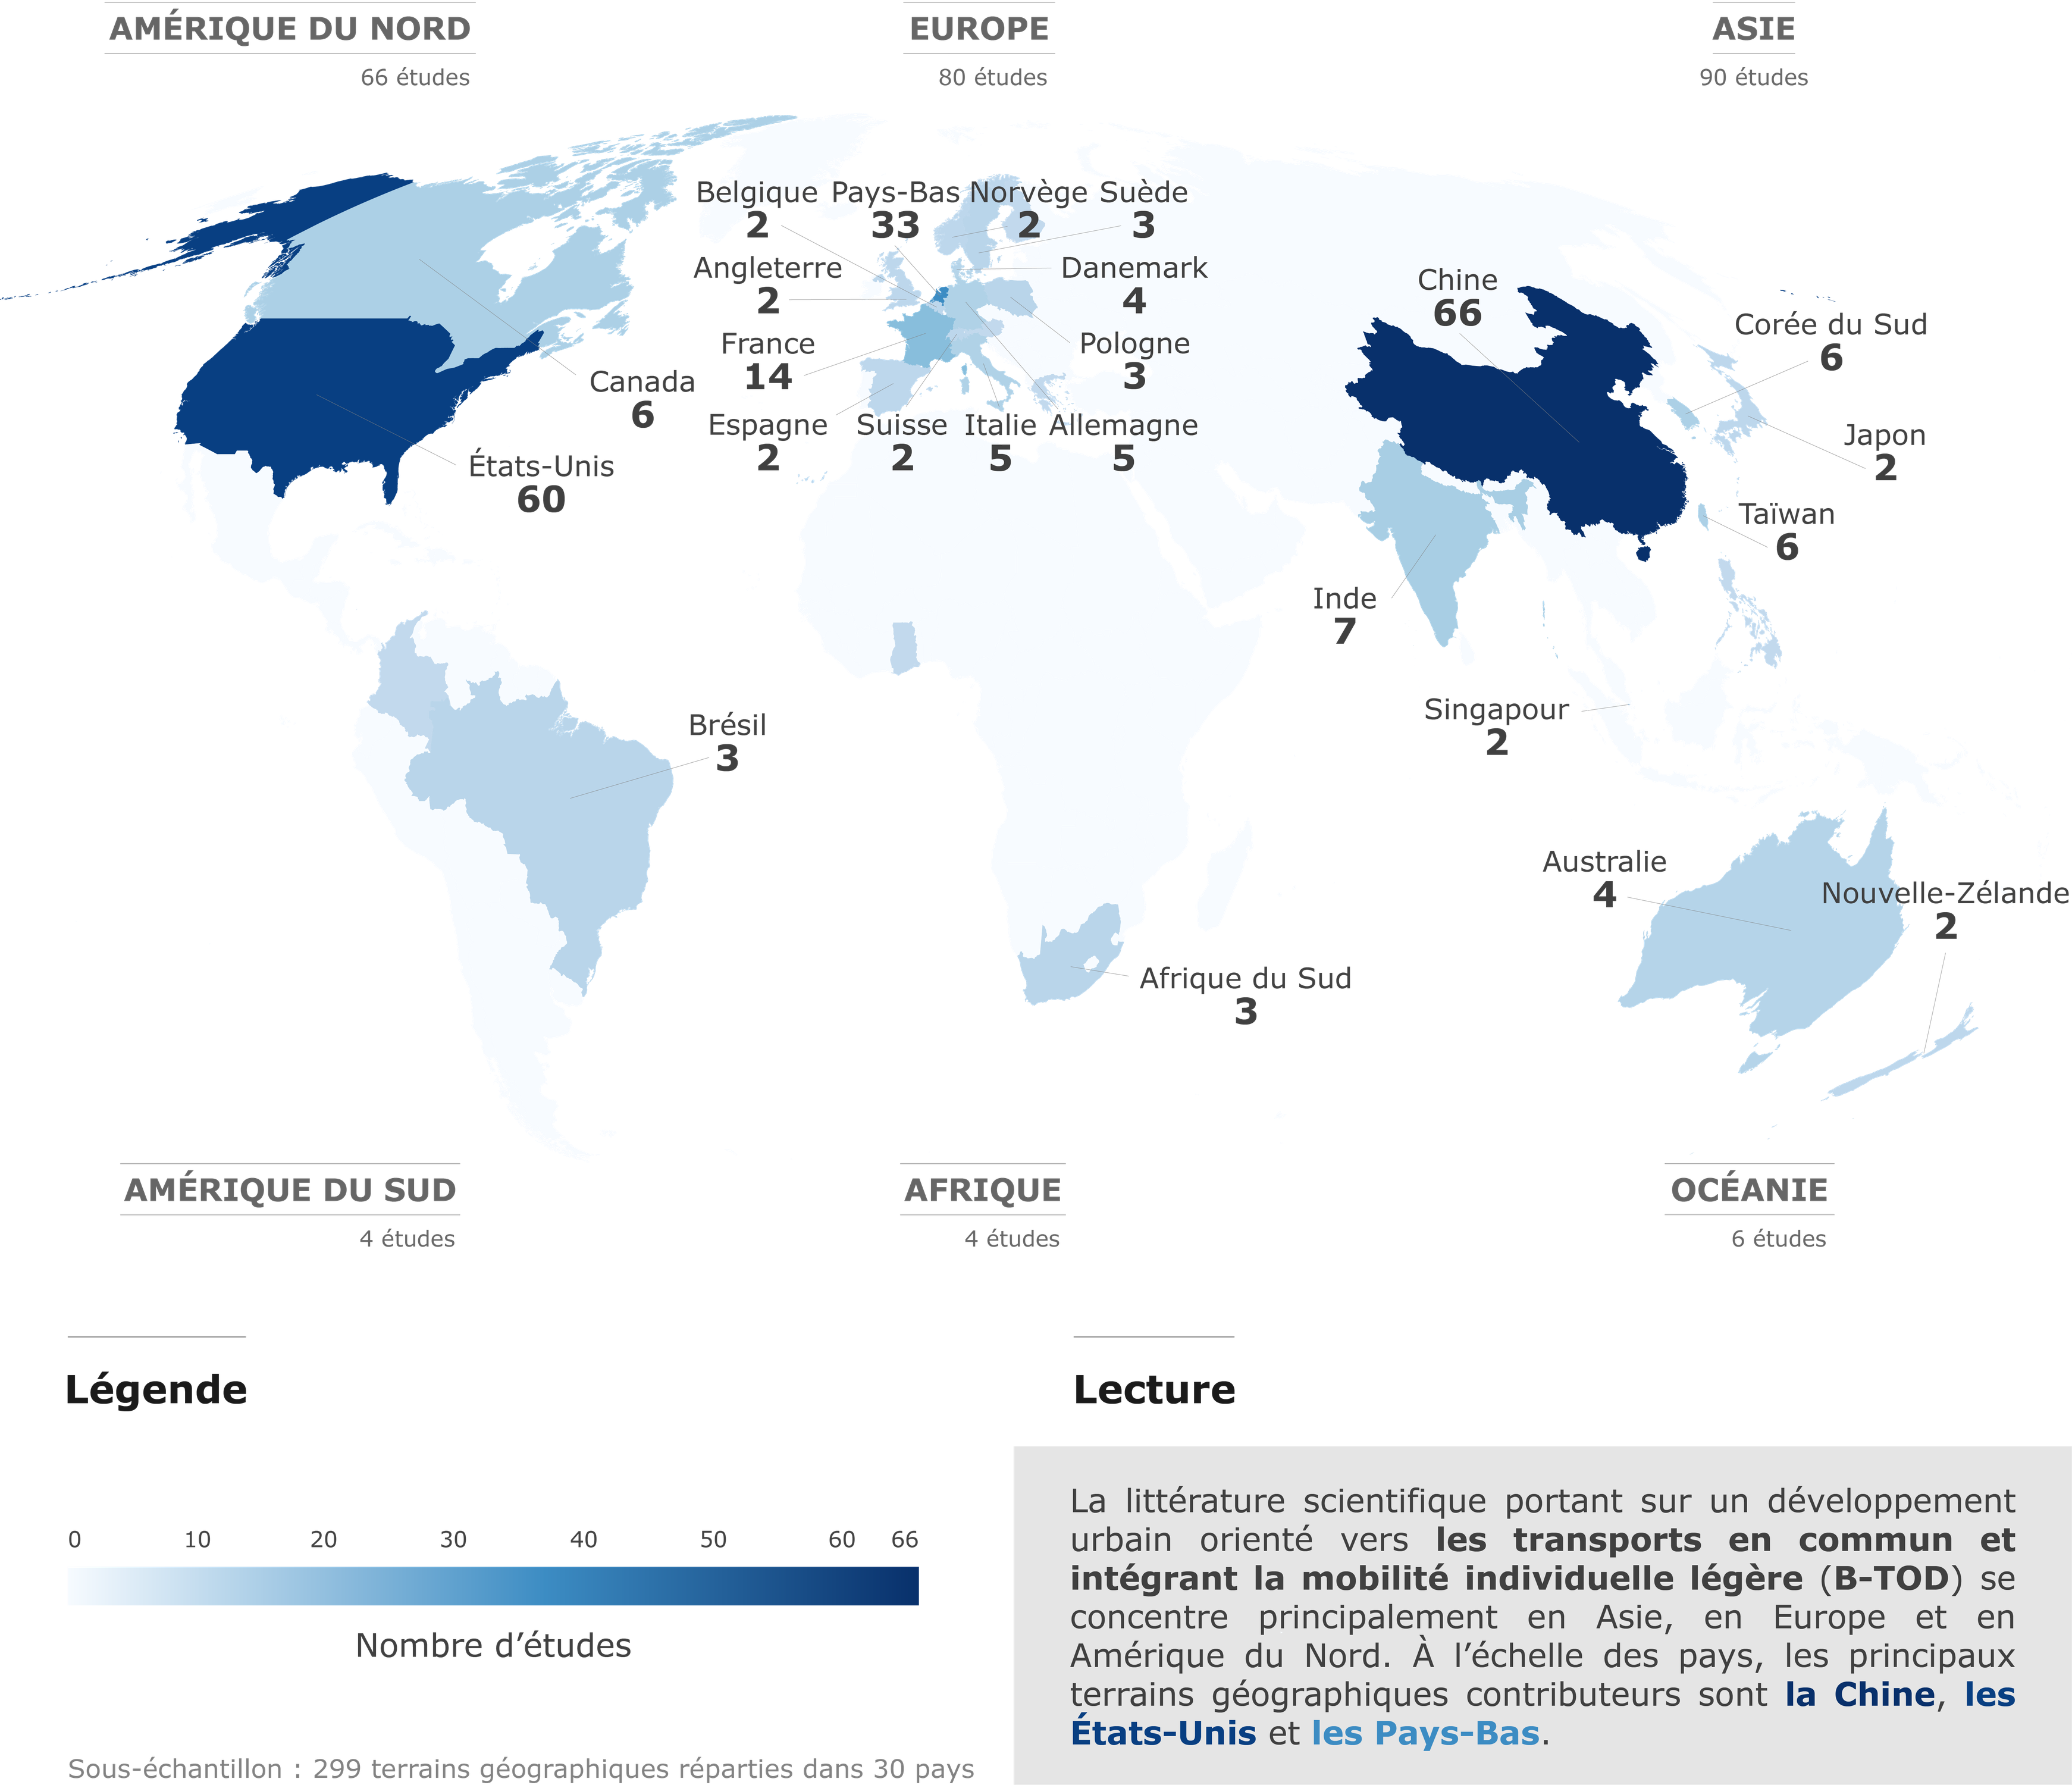
\includegraphics[width=1\columnwidth]{src/Figures/Chap-2/FR_RSL_Carte_Monde.pdf}}
        \vspace{5pt}
        \begin{flushleft}\scriptsize{
        Note~: seuls les pays dont le nombre de contributions est égal ou supérieur à deux sont indiqués sur la carte.
        }\end{flushleft}
        \begin{flushright}\scriptsize{
        Auteur~: \textcolor{blue}{Dylan Moinse (2023)}
        }\end{flushright}
    \end{carte}

    % Répartition géographique par pays
À une échelle plus fine, les pays les plus représentés dans la \acrshort{RSL} consacrée au \acrshort{M-TOD} sont la Chine et les États-Unis, suivis par les Pays-Bas, concordant avec les lieux d'activités répertoriés des chercheur·se·s dans la \hyperref[chap2:analyse-bibliometrique]{sous-section~2.1.1.} (page~\pageref{chap2:analyse-bibliometrique}). À eux seuls, ces trois pays représentent 63,6~\% des terrains géographiques considérés dans les travaux de recherche. Quant au tiers résiduel, cette part est distribuée entre une mosaïque de pays, tantôt industrialisés, tantôt émergents, et incluant la France, l'Inde, la Corée du Sud, Taïwan, le Canada, l'Allemagne et l'Italie (voir la \hyperref[fig-chap2:terrains-geographiques-continents]{carte ~\ref{fig-chap2:terrains-geographiques-continents}}, page~\pageref{fig-chap2:terrains-geographiques-continents}). En conséquence, il conviendrait, dans une formulation plus précise, de parler de l'Europe occidentale, l'Amérique septentrionale et l'Asie orientale en tant qu'entités géographiques manifestement prévalentes au sein de cette \acrshort{RSL}. Ce constat s'aligne sur la revue de littérature, produite par \textcolor{blue}{Bárbara} \textcolor{blue}{\textcite[17]{jansson_almeida_alternativas_2022}}\index{Jansson Almeida, Bárbara|pagebf}, sur l'agencement du vélo avec le métro et qui décrit la place conséquente des études réalisées en Chine, aux Pays-Bas et aux États-Unis. L'analyse du corpus à l'échelle des agglomérations et des communes révèle une concentration autour des mégapoles, principalement en Asie et aux États-Unis. Les régions globalisées le long du littoral chinois, telles que Beijing, Nanjing, Shanghai et Shenzhen, dominent ce classement. Aux États-Unis, des pôles urbains internationaux tels que Washington~D.C., Boston et New York City figurent également en bonne place. En Europe, les points focaux se déplacent vers des centralités régionales, notamment La Haye et Amsterdam (voir la \hyperref[fig-chap2:terrains-geographiques-villes]{carte~\ref{fig-chap2:terrains-geographiques-villes}}, page~\pageref{fig-chap2:terrains-geographiques-villes}). %%Rédigé%%

    % Carte terrains géographiques villes
    \begin{carte}[h!]\vspace*{4pt}
        \caption{Répartition géographique des principales agglomérations examinées dans la revue systématique de la littérature.}
        \label{fig-chap2:terrains-geographiques-villes}
        \centerline{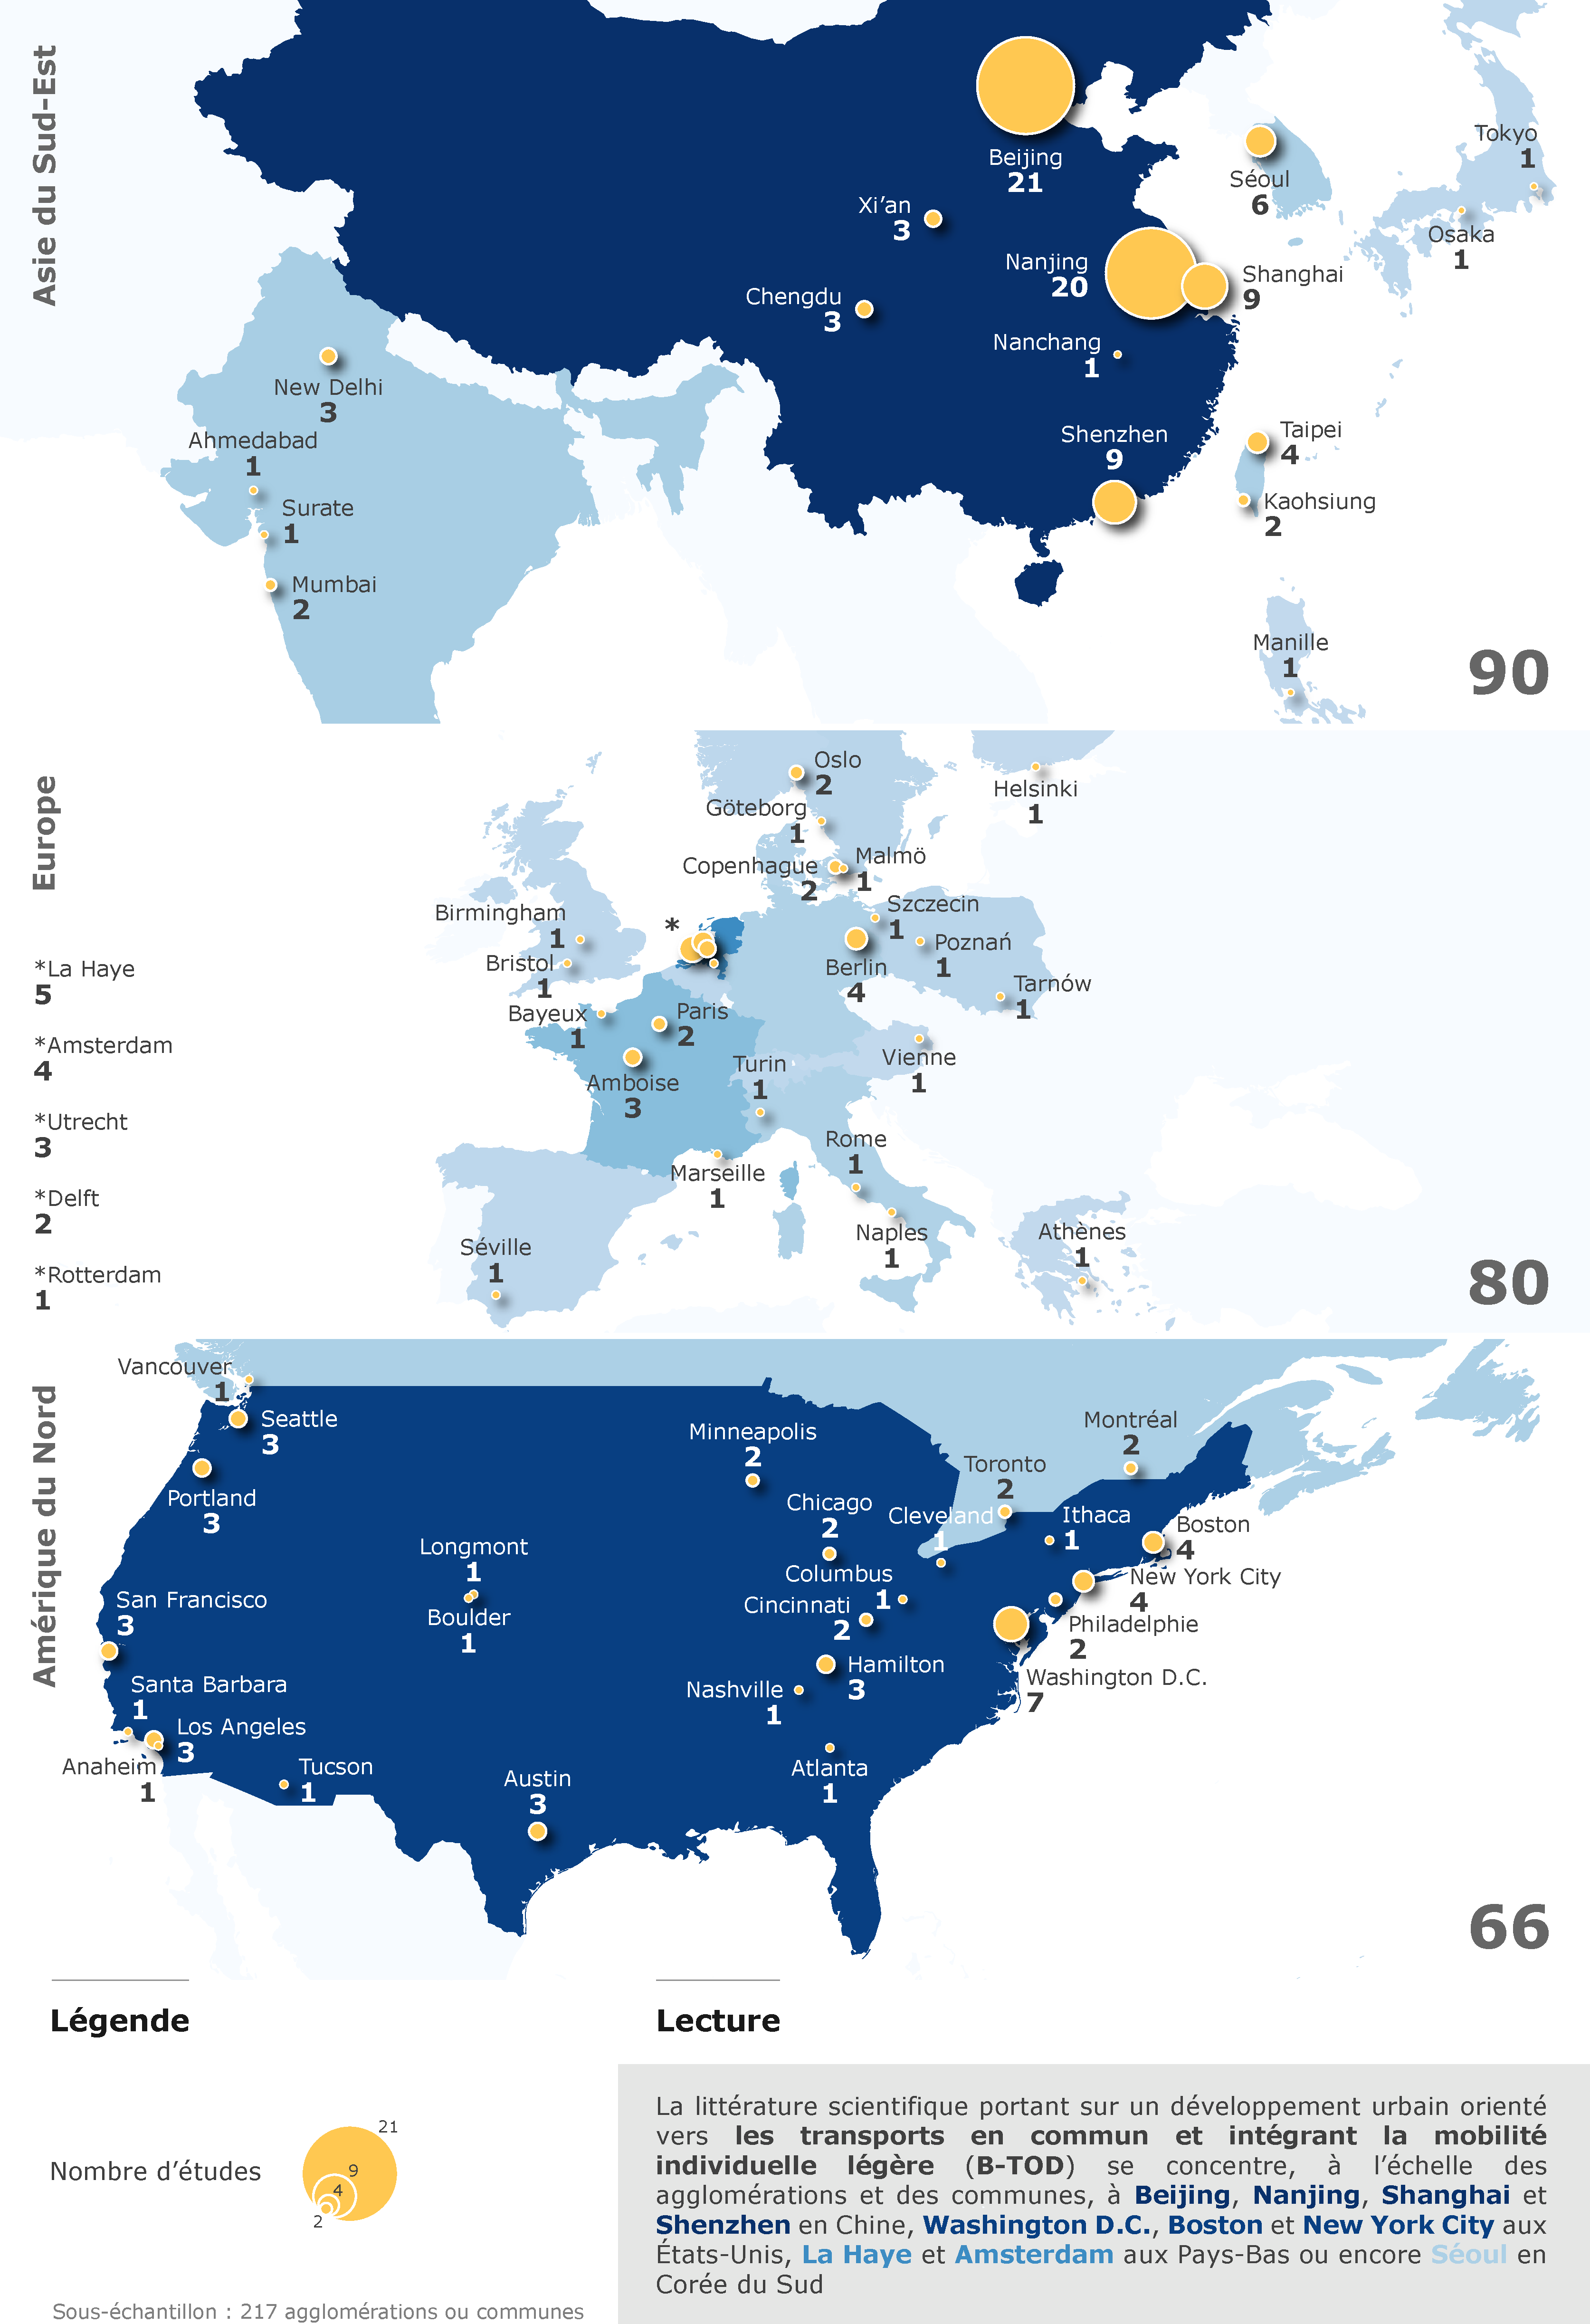
\includegraphics[width=1\columnwidth]{src/Figures/Chap-2/FR_RSL_Carte_Villes.pdf}}
        \vspace{5pt}
        \begin{flushleft}\scriptsize{
        Note~: la somme des contributions associée à chaque pays et continent peut être supérieure aux valeurs propres à chaque agglomération et commune, du fait de productions empiriques ayant adopté une échelle nationale.
        }\end{flushleft}
        \begin{flushright}\scriptsize{
        Auteur~: \textcolor{blue}{Dylan Moinse (2023)}
        }\end{flushright}
    \end{carte}

    % micro-mobilités et TC par continent
Un second aspect auquel s'attache cette section repose sur les formes d'intermodalité étudiées dans la documentation analysée. Comme le montrent les distributions affichées dans la \hyperref[fig-chap2:MIL-TC-continents]{carte~\ref{fig-chap2:MIL-TC-continents}} (page~\pageref{fig-chap2:MIL-TC-continents}), les diverses catégories de mobilité individuelle légère et de transports en commun sont soumises à des investigations inégalitaires, tributaires à des zones géographiques données. Premièrement, la mobilité individuelle légère émergente est bien plus présente en Asie, concernant le vélopartage, et en Amérique du Nord, pour ce qui est des services de trottinettes électriques. Les publications scientifiques élisant un terrain européen s'intéressent principalement au vélo classique. Deuxièmement, les recherches portées sur les systèmes de transport en commun urbain se concentrent également en Asie, principalement avec le métro, et en Amérique du Nord, pour le métro, le tramway et le bus. À l'échelle nationale, il en ressort que certains pays se spécialisent dans des formes d'intermodalité spécifiques. Au sujet du vélo et de la micro-mobilité, nous pouvons notamment retenir la liste de pays suivante~:
    \begin{customitemize}
        \item Dans le contexte des 126 sites d'enquête sur le vélo personnel, nous en comptons 29 aux États-Unis, 28 aux Pays-Bas, 15 en Chine, 11~en France, 6 en Inde et 4 au Canada. De plus, 3 études de cas chacune sont recensées en Afrique du Sud, en Allemagne, en Australie, au Brésil, au Canada, au Danemark et en Italie~;
        \item Sur les 60~lieux abordant le \acrshort{VLS}, 21~d'entre eux sont en Chine, 17 aux États-Unis, 5 à Taïwan et 3 respectivement en Corée du Sud et aux Pays-Bas~;
        \item En ce qui concerne la liste des 44 études de cas sur le \acrshort{VFF}, trois pays seulement sont concernés~: 37 d'entre elles sont situées en Chine, 5 aux États-Unis et 2~aux Pays-Bas~;
        \item Parmi les 20~recherches empiriques focalisées sur le système de \acrshort{TEFF}, 13 d'entre elles se concentrent aux États-Unis et 2~en Allemagne.
    \end{customitemize}
Cette analyse statistique peut être mise en parallèle avec la \acrshort{RSL} menée par \textcolor{blue}{\textcite[298]{zhang_built_2023}}\index{Zhang, Yushan|pagebf}\index{Kasraian, Dena|pagebf}\index{Wesemael, Pieter van|pagebf} sur la mobilité individuelle légère et qui fait état d'une plus grande proportion d'études sur le système de \acrshort{TEFF} en Europe et sur le \acrshort{VLS} et le \acrshort{VFF} en Asie, s'expliquant par des marchés respectivement développés.%%Rédigé%%

    % Figure MIL et TC par continents
    \begin{figure}[h!]\vspace*{4pt}
        \caption{Formes de mobilité individuelle légère et de transports en commun évaluées dans la revue systématique de la littérature, en fonction des continents.}
        \label{fig-chap2:MIL-TC-continents}
        \centerline{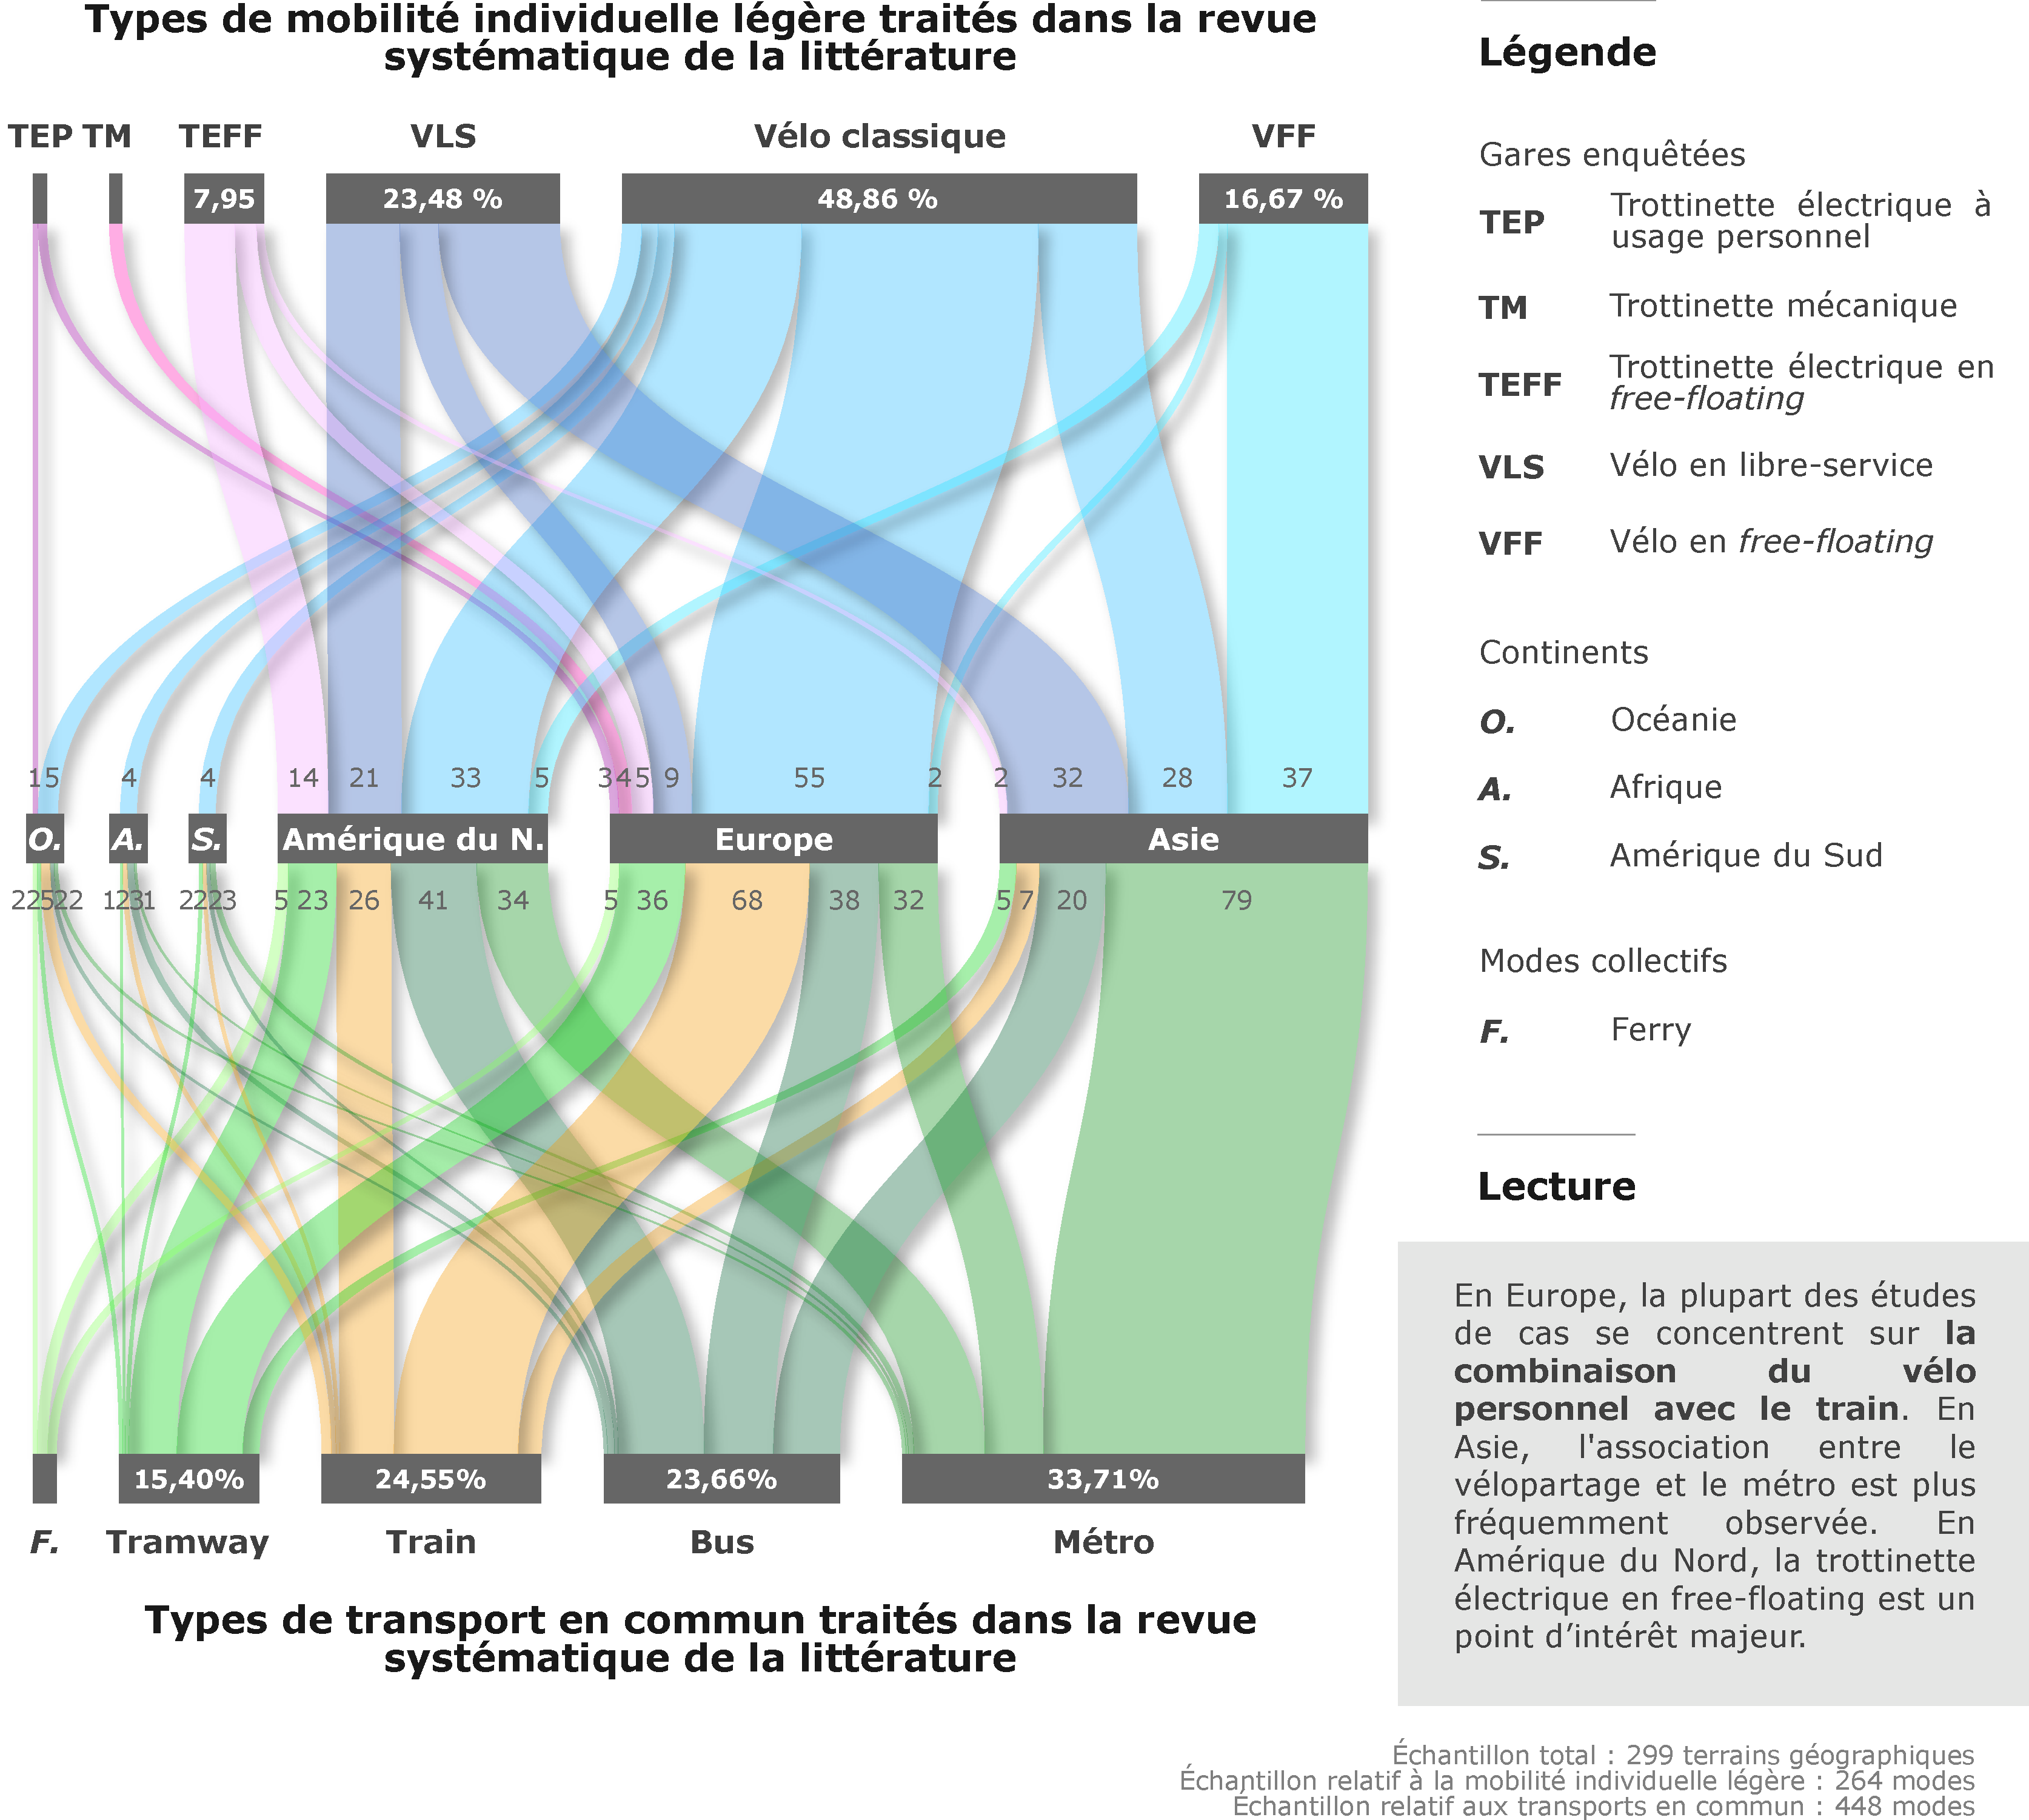
\includegraphics[width=1\columnwidth]{src/Figures/Chap-2/FR_RSL_MIL_TC_Continents.pdf}}
        \vspace{5pt}
        \begin{flushright}\scriptsize{
        Auteur~: \textcolor{blue}{Dylan Moinse (2023)}
        %\\
        %Réalisation avec \Marque{Python}~et sur \Marque{Illustrator}
        }\end{flushright}
    \end{figure}
    
     % TC multimodalité
Bien que la délimitation discernable entre les différents systèmes de transport en commun soit ambivalente lorsqu'il s'agit de procéder à une comparaison internationale\footnote{
    L'ambiguïté entre métro et train dans une perspective de comparaison internationale est inévitable en raison des différences géographiques, culturelles et d'approche en matière de transport. Les tendances et les préférences locales, ainsi que les évolutions technologiques et urbanistiques, peuvent contribuer à brouiller les lignes entre le métro et le train, en particulier lorsqu'il s'agit de comparer différentes régions.
}, il n'en demeure pas moins qu'une proportion substantielle des contributions académiques se livre à une investigation simultanée de divers modes de transport collectif. Force est de constater que, parmi les études analysées, le bus fait l'objet d'un examen dans 66 publications scientifiques, de la même manière que le métro (55 occurrences), le tramway (53 occurrences) et le train (51~occurrences), lorsqu'ils sont envisagés conjointement avec d'autres modes de transport en commun. Quant au ferry, ce mode maritime s'inscrit en une constante imbrication avec d'autres modes collectifs. Sur les 72~documents s'intéressant à plusieurs modes collectifs simultanément, 23 d'entre eux se réfèrent aux États-Unis, tandis que 9 trouvent leur origine en Chine, et que la France et les Pays-Bas y contribuent en parts égales à hauteur de 6 études respectives.%%Rédigé%%

    % Pays minoritaires
En qualité de contributions originales provenant des régions peu explorées ou omises par la \acrshort{RSL}, faut-il faire état des productions scientifiques de \textcolor{blue}{\textcite[34]{bechstein_cycling_2010}}\index{Bechstein, Eva|pagebf}, de \textcolor{blue}{\textcite[368]{cooke_relationship_2018}}\index{Cooke, Sean|pagebf}\index{Behrens, Roger|pagebf}\index{Zuidgeest, Mark|pagebf} et de \textcolor{blue}{\textcite[2]{risimati_spatial_2021}}\index{Risimati, Brightnes|pagebf}\index{Gumbo, Trynos|pagebf}\index{Chakwizira, James|pagebf} en Afrique du Sud~; de \textcolor{blue}{\textcite[108]{quarshie_integrating_2007}}\index{Quarshie, Magnus|pagebf}\index{Morrison, Gregory~M.|pagebf}\index{Rauch, Sébastien|pagebf} au Ghana~; de \textcolor{blue}{\textcite[59]{souza_modelling_2017}}\index{Souza, Flavia de|pagebf}\index{La Paix Puello, Lissy|pagebf}\index{Brussel, Mark|pagebf}\index{Orrico, Romulo|pagebf}, d'\textcolor{blue}{\textcite[36]{arias_molinares_bike_2018}}\index{Arias Molinares, Daniela|pagebf}\index{Florez, Josefina|pagebf} et de \textcolor{blue}{\textcite[40]{jansson_almeida_alternativas_2022}}\index{Jansson Almeida, Bárbara|pagebf} au Brésil~; de \textcolor{blue}{\textcite[206]{cervero_influences_2009}}\index{Cervero, Robert|pagebf}\index{Sarmiento, Olga~L.|pagebf}\index{Jacoby, Enrique|pagebf}\index{Gomez, Luis Fernando|pagebf}\index{Neiman, Andrea|pagebf} en Colombie~; d'\textcolor{blue}{\textcite[6]{arbis_analysis_2016}}\index{Arbis, David|pagebf}\index{Hossein Rashidi, Taha|pagebf}\index{Dixit, Vinayak~V.|pagebf}\index{Vandebona, Upali|pagebf}, de \textcolor{blue}{\textcite[2]{weliwitiya_factors_2017}}\index{Weliwitiya, Hesara|pagebf}\index{Rose, Geoff|pagebf}\index{Johnson, Marilyn|pagebf}, de \textcolor{blue}{\textcite[396]{weliwitiya_bicycle_2019}}\index{Weliwitiya, Hesara|pagebf}\index{Rose, Geoff|pagebf}\index{Johnson, Marilyn|pagebf} et de \textcolor{blue}{\textcite[5]{zhang_make_2023}}\index{Zhang, Mengyuan|pagebf}\index{Lee, Jinwoo Brian|pagebf} en Australie~; ou encore d'\textcolor{blue}{\textcite[17-22]{ensor_forecasting_2010}}\index{Ensor, Matt|pagebf}\index{Slason, Jonathan|pagebf}\index{Vallyon, Chris|pagebf} et d'\textcolor{blue}{\textcite[56-64]{ensor_mode_2021}}\index{Ensor, Matt|pagebf}\index{Maxwell,~O.|pagebf}\index{Bruce, Oliver|pagebf} en Nouvelle-Zélande.%%Rédigé%%

    % Périmètres/échelles choisis (international/national/EPCI)
Le regard porté sur la distribution géographique des terrains d'investigation entraîne une réflexion sous-jacente, quant à l'échelle géographique privilégiée par les travaux empiriques. Au sein du corpus bibliographique, embrassant un total de 238 œuvres scientifiques, quatre d'entre elles assument l'absence d'études de cas en adoptant notamment des approches de modélisations mathématiques. Parallèlement, sept autres recherches présentent exclusivement une revue de littérature et mettent alors en confrontation les recherches empiriques antérieures. Ainsi, 82~\% des recherches menées sur le \acrshort{M-TOD} ont élu, pour contexte géographique, un \acrfull{EPCI}, une commune ou un site local. La part restante est partagée par l'échelle nationale, à hauteur de 11~\%, et régionale, cumulant 6~\%\footnote{
    Il faut préciser que cette catégorisation ne prétend à proposer qu'une trame simplifiée des diverses échelles géographiques, divisées entre les échelons nationaux, régionaux, intercommunaux et communaux. Toutefois, cette démarche s'avère sujette à une limitation, étant donné que la délimitation des contours géographiques d'une région et d'une agglomération varie selon les contextes territoriaux et est donc propice à des erreurs de classements. À titre d'exemple, en 2019, la région Île-de-France s'étend sur environ 12~000~kilomètres carrés et abrite 12 millions d'habitant·e·s, tandis que la métropole du Grand New York occupe une superficie de 34 500~kilomètres carrés avec plus de 20~millions d'habitant·e·s.
}. Force est de souligner que la quasi-majorité des états de l'art adoptent quant à eux une échelle nationale en vue de comparer différents territoires. De manière similaire, la \acrshort{RSL} de \textcolor{blue}{\textcite[298]{zhang_built_2023}}\index{Zhang, Yushan|pagebf}\index{Kasraian, Dena|pagebf}\index{Wesemael, Pieter van|pagebf} fait mention d'une part significative de recherches sur la mobilité individuelle légère dont le cadre géographique ne dépasse pas les limites municipales, et à l'inverse une quasi-absence de travaux à une échelle régionale.%%Rédigé%%

    % Types de territoires analysés 1 (métropoles)
En affinant davantage l'échelle géographique de référence, il est intéressant de noter la pluralité des agglomérations examinées au sein de la \acrshort{RSL}, au regard de leurs dimensions respectives. En nous penchant sur la population des zones urbaines\footnote{
    L'approche comparative des populations repose sur une base de données démographique conçue par \textcolor{blue}{\textcite[]{schiavina_ghs-fua_2019}}\index{Schiavina, Marcello|pagebf}\index{Moreno-Monroy, Ana~I.|pagebf}\index{Maffenini, Luca|pagebf}\index{Veneri, Paolo|pagebf}. Il s'agit de données grillagées sur la population permettant de délimiter les \acrfull{ZUF} dans le monde \textcolor{blue}{\autocite[3]{moreno-monroy_metropolitan_2021}}\index{Moreno-Monroy, Ana~I.|pagebf}\index{Schiavina, Marcello|pagebf}\index{Veneri, Paolo|pagebf}.
}, il nous est donné d'observer les trois continents prédominants dans l'étude du \acrshort{M-TOD}. Conformément au \hyperref[table-chap2:tailles-territoires-rsl]{tableau~\ref{table-chap2:tailles-territoires-rsl}} (page~\pageref{table-chap2:tailles-territoires-rsl}), les mégapoles\footnote{
    \Guillemets{Les mégapoles, ou villes géantes, correspondent aux \textsl{megacities} de la terminologie des Nations-Unies. Ce sont les agglomérations urbaines qui concentrent, selon l’ONU, des populations égales ou supérieures à 10~millions d'habitant·e·s.} \textcolor{blue}{\autocite[]{geoconfluences_megapole_2023}}\index{Géoconfluences@\textsl{Géoconfluences}|pagebf}.
} affichant une démographie supérieure à dix millions d'individus comptent pour 43~\% des terrains géographiques présents dans la \acrshort{RSL}. Ce classement est influencé par les investigations situées en Chine (72~\%) et de manière plus générale, en Asie de l'Est et du Sud-Est (88~\%). De façon analogue, les métropoles jouissant d'un rayonnement international et regroupant une population excédant le seuil des trois millions de citadins occupent une place significative parmi les travaux de recherche empiriques (27~\%). Ces centralités urbaines sont essentiellement localisées aux États-Unis (44~\%), spécifiquement en Amérique du Nord (52~\%). Ce phénomène trouve également écho parmi les métropoles d'importance nationale, voire internationale et comprenant plus d'un million d'habitant·e·s. Ces métropoles intermédiaires sont notamment implantées en Europe occidentale à hauteur de 44~\%, et sont majoritaires en élargissant le périmètre au continent européen dans son ensemble (62~\%). C'est ainsi que les trois types d'aires urbaines mentionnées englobent plus de 87~\% des investigations analysées dans le cadre de la \acrshort{RSL}.%%Rédigé%%

    % Tableau types de territoires analysés RSL
% Tableau types de territoires analysés RSL
%%Rédigé%%
        \begin{table}[h!]
    \centering
    \renewcommand{\arraystretch}{1.5}
    \resizebox{\columnwidth}{!}{
    \begin{tabular}{p{1\columnwidth}}
        %\hline
    \rule{0pt}{15pt} \small{\textbf{\textcolor{blue}{Agglomérations et communes}}}\\
        \hline
    \small{\textbf{\textcolor{blue}{Plus de 10~000~000 d'habitant·e·s (88 références)}}}\\
\small{Beijing (21), Nanjing (19), Shenzhen (9), Shanghai (9), Séoul (6), New York City (4), Chengdu (3), Los Angeles (3), New Delhi (3), Xi'an (3), Chicago (2), Île-de-France (2), Mumbai (2), Bogotá (1), Johannesbourg-Pretoria (1), Osaka (1), Manille (1), Rio de Janeiro (1)}\\
        \hdashline
    \small{\textbf{\textcolor{blue}{Entre 3~000~000 et 10~000~000 d'habitant·e·s (53 références)}}}\\
\small{Washington D.C. (7), Berlin (4), Boston (4), Taipei (4), San Francisco (3), Seattle (3), Suzhou (3), Kaohsiung (2), Melbourne (2), Minneapolis (2), Montréal (2), Philadelphie (2), Toronto (2), Accra (1), Ahmedabad (1), Athènes (1), Atlanta (1), Birmingham (1), Boulder (1), Cape Town (1), Nanchang (1), Porto Alegre (1), Rome (1), Surate (1), Sydney (1), Vienne (1)}\\
        \hdashline
    \small{\textbf{\textcolor{blue}{Entre 1~000~000 et 3~000~000 d'habitant·e·s (33 références)}}}\\
\small{Rotterdam-La Haye (6), Amsterdam (4), Austin (3), Cincinnati (2), Cleveland (2), Copenhague (2), Oslo (2), Auckland (1), Bristol (1), Columbus (1), Helsinki (1), Gutenberg (1), Aix-Marseille-Provence (1), Nashville (1), Orlando (1), Poznań (1), Séville (1), Tucson (1), Turin (1)}\\
        \hdashline
    \small{\textbf{\textcolor{blue}{Entre 250~000 et 1~000~000 d'habitant·e·s (16 références)}}}\\
\small{Hamilton (3), Portland (3), Utrecht (3), Delft (2), Amstelland-Meerlanden (1), Eindhoven (1), Malmö (1), Mamelodi (1), Tarnow (1)}\\
        \hdashline
    \small{\textbf{\textcolor{blue}{Moins de 250~000 habitant·e·s (8 références)}}}\\
\small{Amboise (3), Bayeux (1), El Monte (1), Ithaca (1), Longmont (1), communes belges entre 30~000~et 200~000~habitant·e·s (1)}\\
        \hline
        \end{tabular}}
    \caption{Taille des agglomérations et des communes étudiées dans la revue systématique de la littérature.}
    \label{table-chap2:tailles-territoires-rsl}
        \vspace{5pt}
        \begin{flushleft}\scriptsize{
        \textcolor{blue}{Lecture~:} à partir de 198 études comprenant un terrain géographique, la revue systématique de la littérature est principalement composée d'agglomérations de plus de 3~000~000 d'habitant·e·s.
        }\end{flushleft}
        \begin{flushright}\scriptsize
        Auteur~: \textcolor{blue}{Dylan Moinse (2023)}
        \end{flushright}
        \end{table}%%Rédigé%%

    % Types de territoires analysés 2 (métropoles régionales)
En ce qui concerne les agglomérations peuplées de moins d'un million d'habitant·e·s, les études de cas en milieu urbain s'articulent principalement autour des intercommunalités néerlandaises, spécifiquement dans les localités de Delft \textcolor{blue}{\autocites[113]{heinen_multimodal_2014}[5]{molin_bicycle_2015}}\index{Heinen, Eva|pagebf}\index{Bohte, Wendy|pagebf}\index{Molin, Eric|pagebf}\index{Maat, Kees|pagebf}, d'Amstelland-Meerlanden \textcolor{blue}{\autocite[46]{brand_assessing_2015}}\index{Brand, Judith Caroline|pagebf}, d'Eindhoven \textcolor{blue}{\autocite[724]{waerden_relation_2018}}\index{Waerden, Peter|pagebf}\index{Waerden, Jaap|pagebf} et d'Utrecht \textcolor{blue}{\autocite[289]{kuijk_preferences_2022}}\index{Mil, Joeri~F.P. van|pagebf}\index{Leferink, Tessa~S.|pagebf}\index{Annema, Jan Anne|pagebf}\index{Oort, Niels van|pagebf}\index{Kuijk, Roy~J. van|pagebf}\index{Almeida Correia, Gonçalo Homem de|pagebf}\index{Oort, Niels van|pagebf}\index{Arem, Bart van|pagebf}. Les États-Unis constituent également un terrain propice à ce sujet de recherche, à travers des travaux prenant appui à Portland \textcolor{blue}{\autocites[164]{krizek_assessing_2011}[400]{mcqueen_assessing_2022}[94]{singleton_exploring_2014}[265]{welch_long-term_2016}[83]{pucher_integrating_2009}}\index{Krizek, Kevin~J.|pagebf}\index{Stonebraker, Eric~W.|pagebf}\index{McQueen, Michael|pagebf}\index{Clifton, Kelly~J.|pagebf}\index{Singleton, Patrick~A.|pagebf}\index{Welch, Timothy~F.|pagebf}\index{Gehrke, Steven~R.|pagebf}\index{Wang, Fangru|pagebf}\index{Pucher, John|pagebf}\index{Buehler, Ralph|pagebf} et à Anaheim, dans la région métropolitaine de Los Angeles (\textsl{Greater Los Angeles Area}), \textcolor{blue}{\autocite[1579]{liu_simultaneous_2015}}\index{Liu, Yang|pagebf}\index{Zhu, Ning|pagebf}\index{Ma, Shou-feng|pagebf}. De même, les territoires canadiens contribuent à cette documentation, à l'aide de publications scientifiques centrées sur la région métropolitaine d'Hamilton \textcolor{blue}{\autocites[2162]{chan_factors_2020}[375]{ravensbergen_biking_2018}}\index{Ravensbergen, Léa|pagebf}\index{Chan, Kevin|pagebf}\index{Farber, Steven|pagebf}\index{Buliung, Ron|pagebf}\index{Mendonca, Meaghan|pagebf}\index{Garg, Naren|pagebf}. Quant aux agencements territoriaux à dominante rurale et périurbaine, les exemples français abondent, marqués par une série d'études menées au sein des communes d'Amboise \textcolor{blue}{\autocites[747]{midenet_modal_2018}[2729]{papon_evaluation_2017}[14-16]{papon_rapport_2015}}\index{Midenet, Sophie|pagebf}\index{Côme, Etienne|pagebf}\index{Papon, Francis|pagebf}\index{Beauvais, Jean-Marie|pagebf}\index{Midenet, Sophie|pagebf}\index{Côme, Etienne|pagebf}\index{Polombo, Nadine|pagebf}\index{Abours, Sylvie|pagebf}\index{Belton-Chevallier, Leslie|pagebf}\index{Soulas, Claude|pagebf} et de Bayeux \textcolor{blue}{\autocite[2]{richer_service_2017}}\index{Richer, Cyprien|pagebf}, ainsi que dans l'ancienne \acrfull{CC} de la Brie Boisée (faisant partie intégrante de l'Île-de-France depuis 2017) mise en perspective avec celle de Carnelle Pays de France et de Haute Vallée de Chevreuse \textcolor{blue}{\autocite[39]{stransky_periurbain_2019}}\index{Stransky, Vaclav|pagebf}.%%Rédigé%%

    % Figure comparaisons internationales
    \begin{figure}[h!]\vspace*{4pt}
        \caption{Comparaisons entre terrains géographiques dans le corpus bibliographique de la revue systématique de la littérature.}
        \label{fig-chap2:comparaisons-internationales-rsl}
        \centerline{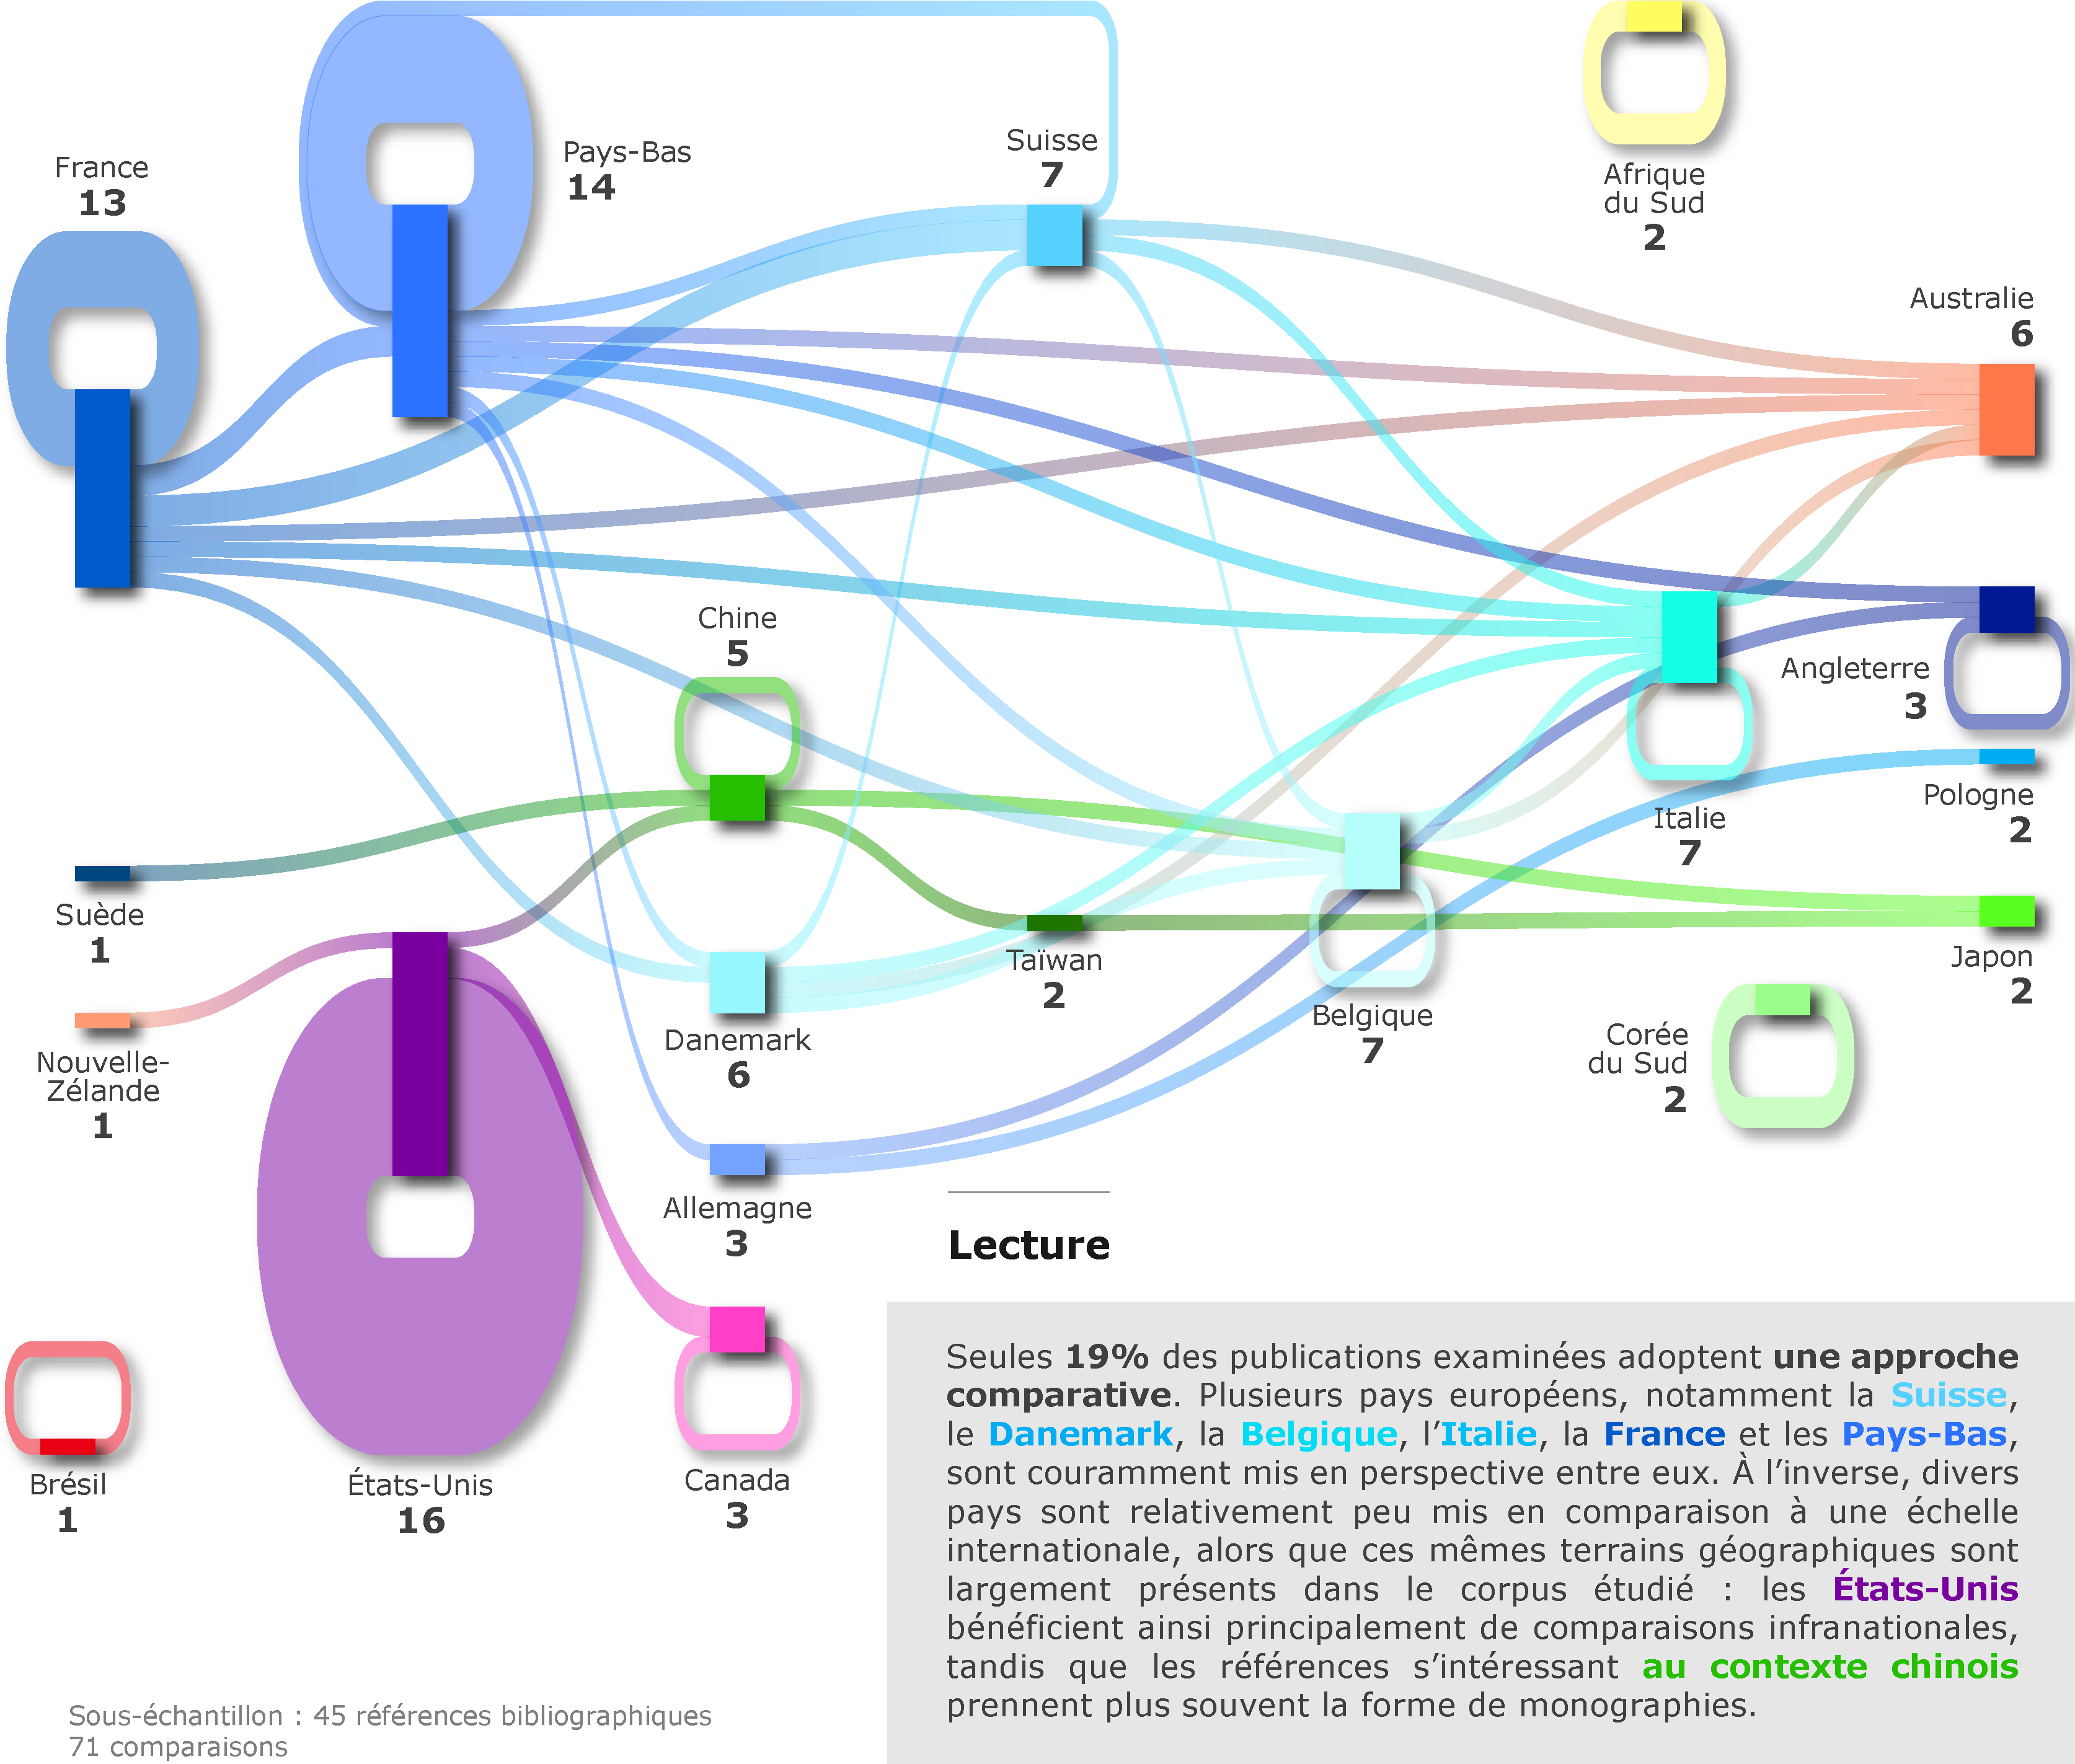
\includegraphics[width=1\columnwidth]{src/Figures/Chap-2/FR_RSL_Comparaisons_internationales.pdf}}
        \vspace{5pt}
        \begin{flushright}\scriptsize{
        %\\
        %Réalisation avec \Marque{Python}~et sur \Marque{Illustrator
        Note~: seules les comparaisons menées entre différentes régions ont été prises en compte afin d'exclure un même périmètre urbain comportant plusieurs sites locaux étudiés. L'anneau correspond à des comparaisons infranationales, tandis que les flux lient les terrains géographiques mis en perspective.
        \\
        Auteur~: \textcolor{blue}{Dylan Moinse (2023)}
        }\end{flushright}
    \end{figure}

    % Comparaisons internationales
Si la documentation relative au \acrshort{M-TOD} adopte communément une approche comparative en sélectionnant divers sites d'étude au sein d'un système politique cohérent, plus rares sont les recherches qui se prêtent à la mise en parallèle de divers territoires répartis dans des pays distincts. En réalité, il ressort que 19~\% des publications examinées se dédient à une comparaison internationale ou infranationale. Dans le sous-ensemble constitué de 45 publications scientifiques consacrées aux comparaisons, 30~d'entre elles opèrent une mise en perspective entre différents \acrshort{EPCI} tandis que 11~autres embrassent l'échelon national. Comme en témoigne l'\hyperref[fig-chap2:comparaisons-internationales-rsl]{illustration~\ref{fig-chap2:comparaisons-internationales-rsl}} (page~\pageref{fig-chap2:comparaisons-internationales-rsl}), certains pays sont fréquemment mis en relation, tels que la Suisse, le Danemark, la Belgique, l'Italie, la France et les Pays-Bas \textcolor{blue}{\autocites[29-46]{abours_rapport_2015}[279-285]{sebban_complementarite_2003}[282-284]{martens_bicycle_2004}}\index{Abours, Sylvie|pagebf}\index{Midenet, Sophie|pagebf}\index{Soulas, Claude|pagebf}\index{Sebban, Annie-Claude|pagebf}\index{Martens, Karel|pagebf}, notamment avec d'autres pays européens~; ou encore le Japon, Taïwan et la Chine \textcolor{blue}{\autocite[212]{lin_built_2018}}\index{Lin, Jen-Jia|pagebf}\index{Zhao, Pengjun|pagebf}\index{Takada, Kazuyuki|pagebf}\index{Li, Shengxiao|pagebf}\index{Yai, Tetsuo|pagebf}\index{Chen, Chi-Hao|pagebf}. Soulignons qu'il existe également deux comparaisons intercontinentales, portées par \textcolor{blue}{\textcite[4]{hamidi_shaping_2020}}\index{Hamidi, Zahra|pagebf}\index{Zhao, Chunli|pagebf} qui ont étudié les aires urbaines chinoises et suédoises de Beijing, Göteborg et Malmö~; et par \textcolor{blue}{\textcite[13]{hua_transfer_2022}}\index{Hua, Mingzhuang|pagebf}\index{Pereira, Francisco Camara|pagebf}\index{Jiang, Yu|pagebf}\index{Chen, Xuewu|pagebf} qui se sont intéressé·e·s aux villes chinoises et étasuniennes de Nanjing et de Chicago.%%Rédigé%%

    % Comparaisons infranationales
Dans le sens contraire, certains pays sont peu mis en perspective, même s'ils sont amenés à être comparés dans de faibles proportions (voir l'\hyperref[fig-chap2:comparaisons-internationales-rsl]{illustration~\ref{fig-chap2:comparaisons-internationales-rsl}}, page~\pageref{fig-chap2:comparaisons-internationales-rsl}). Citons, par exemple, les États-Unis qui, à l'exception de certaines comparaisons avec le Canada \textcolor{blue}{\autocites[11-16]{ensor_forecasting_2010}[7]{schneider_integration_2005}[83]{pucher_integrating_2009}}\index{Ensor, Matt|pagebf}\index{Slason, Jonathan|pagebf}\index{Vallyon, Chris|pagebf}\index{Schneider, Robert|pagebf}\index{Pucher, John|pagebf}\index{Buehler, Ralph|pagebf}, bénéficient principalement de comparaisons infranationales. Certains pays n'ont, par ailleurs, bénéficié que de comparaisons internes entre différentes régions du même ensemble géographique. En Afrique du Sud, \textcolor{blue}{Eva} \textcolor{blue}{\textcite[34]{bechstein_cycling_2010}}\index{Bechstein, Eva|pagebf} opte pour une démarche comparative entre les \Guillemets{\textsl{townships}}\footnote{
    \Guillemets{En Afrique du Sud, depuis l'\textsl{apartheid}, régime de ségrégation raciale, le mot \textsl{township} désigne des quartiers habités par les populations de couleur (noirs et \textsl{coloured}). [\dots] En désignant les quartiers habités par des populations ségrégées, il finit par désigner des quartiers pauvres, d'habitat dégradé et insalubre, se rapprochant de la définition du bidonville.}~\textcolor{blue}{\autocite{geoconfluences_township_2023}}\index{Géoconfluences@\textsl{Géoconfluences}|pagebf}.
} de Mamelodi et de Nellmapius (Tshwane), de la même façon que \textcolor{blue}{\textcite[368]{cooke_relationship_2018}}\index{Cooke, Sean|pagebf}\index{Behrens, Roger|pagebf}\index{Zuidgeest, Mark|pagebf} entre les municipalités métropolitaines de Johannesbourg, Le Cap, Tshwane, la baie Nelson Mandela et d'eThekwini. En Corée du Sud, les recherches menées par \textcolor{blue}{\textcite[43, 980]{lee_strategies_2010, lee_bicycle-based_2016}}\index{Lee, Jaeyeong|pagebf}\index{Shin, Hee-Cheol|pagebf}\index{Lee, Jaeyeong|pagebf}\index{Choi, Keechoo|pagebf}\index{Leem, Yountaik|pagebf} suivent une analyse comparative entre les régions métropolitaines de Séoul et de Daejeon.%%Rédigé%%

    % Peu de comparaisons
À l'inverse, l'\hyperref[fig-chap2:comparaisons-internationales-rsl]{illustration~\ref{fig-chap2:comparaisons-internationales-rsl}} (page~\pageref{fig-chap2:comparaisons-internationales-rsl}) révèle la sous-représentation, voire l'absence, de certains pays qui sont pourtant bien étudiés dans la \acrshort{RSL}. Le cas le plus frappant est celui de la Chine, où la grande majorité des recherches utilise une approche monographique, se concentrant uniquement sur une seule agglomération. Toutefois, il convient de noter que ces études ne sont pas nécessairement non comparatives \textcolor{blue}{\autocite[30-31]{gueranger_monographie_2012}}\index{Guéranger, David|pagebf}. Par exemple, l'étude réalisée par \textcolor{blue}{\textcite[77]{liu_solving_2012}}\index{Liu, Zhili|pagebf}\index{Jia, Xudong|pagebf}\index{Cheng, Wen|pagebf} procède à deux études de cas dans les quartiers de Dongcheng et d'Haidian, à Beijing, après avoir réalisé une analyse exhaustive du système de \acrshort{VLS} autour des arrêts de métro et de bus dans la capitale. En excluant les comparaisons au sein d'une même aire urbaine du fait de contraintes méthodologiques liées à la normalisation des terrains géographiques, ce graphique masque le raisonnement analogique présent à l'échelle infracommunale.%%Rédigé%%

    % Conclusion
En somme, cette section consacrée à l'état de la littérature scientifique internationale sur le \acrshort{M-TOD} s'est à la fois penchée sur l'analyse des métadonnées des publications scientifiques collectées, les schémas lexicaux utilisés pour décrire le sujet de recherche, ainsi que sur les tendances chronologiques et la répartition géographique des investigations conduites. Après avoir analysé la documentation sous l'angle des métadonnées, la section suivante abordera les cadres conceptuels et méthodologiques de la littérature scientifique sur le \acrshort{M-TOD}, en portant un regard sur les fondements théoriques, l'évaluation des démarches et sur les types d'analyse employés au sein des investigations.%%Rédigé%%

    % 2.2.2. concepts, méthodes, types d'analyse
    \needspace{1\baselineskip} % Réserve de l'espace
\subsection{Cadres conceptuels et méthodologiques du corpus
    \label{chap2:cadres-conceptuels-methodologiques}
    }
    
    % Introduction
Cette partie est dédiée à la présentation et à la mise en confrontation des divers fondements théoriques et des démarches employés dans la littérature scientifique. Les questionnements suivants ont été considérés dans cette analyse~:
    \begin{customitemize}
        \item Quels sont les principaux cadres théoriques mobilisés dans la documentation sélectionnée~? De quelle manière ces choix théoriques ont-ils été appliqués aux questions de recherche~?
        \item Peut-on identifier des évolutions des cadres théoriques adoptés au fil du temps~? Ces tendances reflètent-elles certaines orientations ou avancées disciplinaires~? Quelles critiques ont été soulevées par les auteurs concernant les cadres théoriques utilisés~?
        \item Quelles méthodes de collecte de données ont été utilisées~? Quelles techniques d'analyse des données ont été appliquées~?
        \item Comment les auteur·rice·s ont-ils abordé les contraintes et les limites des méthodes de collecte et d'analyse utilisées~?
    \end{customitemize}%%Rédigé%%

    % Annonce du plan
Cette sous-section se propose d'introduire les cadres théoriques inscrits dans la littérature scientifique (\hyperref[chap2:fondements-theoriques]{sous-section~2.2.1}, page~\pageref{chap2:fondements-theoriques}), préalablement à l'évaluation des procédés de collecte de données (\hyperref[chap2:methodes-collecte-donnees]{sous-section~2.2.2}, page~\pageref{chap2:methodes-collecte-donnees}) et des méthodes d'analyse des données (\hyperref[chap2:demarches-types-analyses]{sous-section~2.2.3}, page~\pageref{chap2:demarches-types-analyses}) employées pour étudier le \acrshort{M-TOD}.%%Rédigé%%

    % 2.2.2.1. Concepts mobilisés, TOD
    \needspace{1\baselineskip} % Réserve de l'espace
\subsubsection*{Fondements théoriques
    \label{chap2:fondements-theoriques}
    }
    
    % Cadres théoriques description
Dans l'ensemble des 102~articles scientifiques analysés dans le cadre de la \acrshort{RSL}, le concept de \acrshort{TOD} est prédominant, étant cité dans 55 études. Parmi ces travaux, 53 articles discutent explicitement du \acrshort{TOD}, avec neuf d'entre eux s'appuyant spécifiquement sur les principes des \Guillemets{Ds} pour structurer leur analyse. Quatre études se fondent sur une approche analytique des \Guillemets{5Ds}, trois sur les \Guillemets{3Ds}, une sur les \Guillemets{4Ds} et une autre sur les \Guillemets{6Ds}\footnote{
    Dans l'ordre communément accepté dans la littérature scientifique portant sur le \acrshort{TOD}, et comme présenté dans la \hyperref[chap1:tod-presentation-generale-definition]{section sur la définition du \textsl{Transit-Oriented Development}} (page~\pageref{chap1:tod-presentation-generale-definition}) du \hyperref[chap1:titre]{chapitre~1} (page~\pageref{chap1:titre}), les \Guillemets{\acrshort{7Ds}} se composent de la façon suivante~: la \Guillemets{densité} (\textsl{Density}, \(D1\)), la \Guillemets{diversité fonctionnelle} (\textsl{Diversity}, \(D2\)), le \Guillemets{traitement des espaces publics} (\textsl{Design}, \(D3\)), l'\Guillemets{accessbilité aux destinations} (\textsl{Destination Accessibility}, \(D4\)), l'\Guillemets{accessbilité locale} (\textsl{Distance to Transit}, \(D5\)), le \Guillemets{management de la demande de mobilité} (\textsl{Demand Management}, \(D6\)) et les \Guillemets{caractéristiques socio-démographiques} (\textsl{Demographics}, \(D7\)).
}. Quatre articles intègrent une version revisitée du \acrshort{TOD} qui fait fortement écho au présent chapitre, portant sur le \acrshort{M-TOD}. La place importante du \acrshort{TOD} dans la littérature est néanmoins influencée par son intégration dans notre formule de recherche lors de la collecte des bases de données. Outre le \acrshort{TOD}, deux autres notions émergent fréquemment~: les \Guillemets{premiers et derniers kilomètres}, mentionnés 24 fois, et l'\Guillemets{accessibilité multimodale}, évoquée dans 20~articles. D'autres concepts sont également présents, tels que la \Guillemets{dépendance automobile} (quatre mentions), le \Guillemets{\acrfull{MaaS}} (quatre mentions), l'\Guillemets{inclusivité sociale} (quatre mentions) et la \Guillemets{théorie du comportement planifié} (deux mentions).%%Rédigé%%

    % Focus M-TOD
En réalité, un nombre important de publications aborde le concept de \acrshort{TOD} sans le mentionner explicitement. De même, bien que rarement cité, le concept de \acrshort{M-TOD} est intrinsèquement lié au corpus académique qui examine l'intégration de la mobilité individuelle légère avec les réseaux de transport en commun, tout en articulant les problématiques liées à la mobilité et à la fabrique urbaine. En premier lieu, faut-il alors mentionner l'étude de \textcolor{blue}{\textcite{lee_bicycle-based_2016}}\index{Lee, Jaeyeong|pagebf}\index{Choi, Keechoo|pagebf}\index{Leem, Yountaik|pagebf} à l'origine de la conceptualisation du \acrshort{B-TOD} et prenant appui sur une investigation explorant la relation entre le vélo et le métro à Séoul et à Daejeon. Par ailleurs, trois recherches employant le \acrshort{B-TOD} se concentrent sur différents objets et contextes géographiques~: l'une à Nanjing examinant le vélo, le \acrshort{VLS} et le métro \textcolor{blue}{\autocite{ji_public_2017}}\index{Ji, Yanjie|pagebf}\index{Fan, Yingling|pagebf}\index{Ermagun, Alizera|pagebf}\index{Cao, Xuening|pagebf}\index{Wang, Wei|pagebf}\index{Das, Kirti|pagebf}~; une autre à Kaohsiung entre le \acrshort{VLS} et le métro \textcolor{blue}{\autocite{cheng_expanding_2018}}\index{Cheng, Yung-Hsiang|pagebf}\index{Li, Yi-Chun|pagebf}~; et la dernière étudiant le lien entre le vélo et le bus dans les villes de Cape Town, Tshwane, Joburg, Nelson Mandela Bay et eThekwini \textcolor{blue}{\autocite{cooke_relationship_2018}}\index{Cooke, Sean|pagebf}\index{Behrens, Roger|pagebf}\index{Zuidgeest, Mark|pagebf}. La diversité des approches théoriques adoptées se reflète dans la pluralité méthodologique destinée à explorer les interactions entre le vélo, la micro-mobilité et le transport public.%%Rédigé%%

    % 2.2.2.2. méthodes, sources de données et échantillon
    \needspace{1\baselineskip} % Réserve de l'espace
\subsubsection*{Évaluation des méthodes de collecte des données
    \label{chap2:methodes-collecte-donnees}
    }
    
    % Sources de données détaillées : big data
Le travail d'analyse des sources de données utilisées dans la documentation a mené à l'identification de 17 types de méthodes de collecte, classées en cinq catégories indépendantes. La majorité des productions scientifiques a recours à l'exploitation des données ouvertes (29,15~\%) et des données d'usage (23,87~\%) que nous pouvons regrouper sous l'objet technique de la \textsl{Big Data}\footnote{
    Dans le contexte de la mobilité, la \textsl{Big Data} ou mégadonnées fait référence à la collecte et au traitement d'une base de données publique ou privée générée par un système de transport, de véhicule, par les utilisateur·rice·s eux-mêmes ou par d'autres sources mises à disposition. Cette technique de recueil de données quantitatives en temps réel est notamment permise par l'émergence de technologies telles que les capteurs embarqués dans les véhicules, les compteurs, les smartphones ou encore le déploiement d'outils numériques.
}, suivies par la réalisation d'enquêtes (24,62~\%) et d'analyses secondaires à partir de bases de données (16,58~\%). Les flux de mobilité mis à disposition en ligne représentent ainsi 53,02~\% des sources de données mobilisées et correspondent principalement à l'\textsl{Open Data}\footnote{
    L'\textsl{Open Data} se réfère, dans le cas particulier de cette \acrshort{RSL}, à la politique de mise à disposition publique de données liées à l'urbanisme et à la mobilité. Ces données ouvertes et diffusées par les collectivités territoriales et par des organismes publics comprennent une variété d'informations relatives à l'aménagement urbain, à l'utilisation des sols, aux infrastructures, à la démographie et à d'autres aspects de la gestion territoriale.
} (22,54~\%), à l'\acrfull{API}\footnote{
    Une \acrshort{API} est une interface informatique qui met en relation les applications et les services avec les systèmes de mobilité, de manière standardisée. Les \acrshort{API} facilitent alors l'échange de données entre les fournisseurs de services de mobilité et les applications tierces, à l'image de la localisation, l'état et la disponibilité des véhicules en temps réel, le déverrouillage des véhicules ainsi que le processus facturation pour un trajet effectué. L'ensemble des données générées et échangées permettent aux entreprises d'accéder aux données agrégées sur l'utilisation des véhicules et pouvoir les intégrer.
} (11,72~\%) et aux flux de mobilité liés aux systèmes de \acrshort{VLS}, appelés \acrfull{GBFS}\footnote{
    Les \acrshort{GBFS} définissent un format standardisé de données spécifiquement conçu pour les systèmes de \acrshort{VLS}, dans le but de fournir des informations en temps réel sur le service de mobilité et de favoriser l'interopérabilité et la transparence.
} (9,02~\%) et de transport en commun, \acrfull{GTFS}\footnote{
    Les \acrshort{GTFS} constituent un format de fichier standardisé, initialement baptisé \Guillemets{\textsl{Google Transit Feed Specification}}, et servant à la description des réseaux de transport en commun. Ces informations comprennent notamment les itinéraires, les points d'arrêt, les plages horaires ainsi que les données de fréquentation. Cette normalisation a pour finalité de faciliter l'intégration de ces données ouvertes dans les outils de \gls{cartographie} et de planification d'itinéraires. À ce titre, les organismes de transport en commun mettent à disposition ces formats uniformisés, visant aussi bien les développeur·se·s d'applications tierces que les usager·ère·s.
} (6,85~\%). Nous retrouvons également certaines techniques de collecte de données classées parmi les données ouvertes et d'usage, telles que l'extraction de données de mobilité issues des cartes multimodales, de l'ordre de 2,16~\%, ou de données \acrshort{GPS} (\textsl{Global Positioning System}), à hauteur de 1,89~\%.%%Rédigé%%

    % Sources de données détaillées : méthodes qualitatives
Au-delà de cette méthode de recueil liée à la \textsl{Smart Data}, émane un second éventail associé aux enquêtes de terrain, par le biais du questionnaire (20,47~\%), de l'entretien (2,80~\%) et de l'observation (1,98~\%). Ces techniques ancrées dans les pratiques de recherche de la géographie et de la sociologie sont impulsées par la mise en œuvre de questionnaires en ligne (11,45~\%), en face-à-face (7,66~\%) et par courrier (1,35~\%) ainsi que d'entretiens menés individuellement (1,71~\%) ou collectivement (1,08~\%) et de séances d'observation directe (1,98~\%). La pluralité des méthodes de collecte de données se traduit, en dernier lieu, par l'exploitation et la réinterprétation d'enquêtes publiques préexistantes (14,52~\%) et par l'exercice de mise en synthèse de matériaux antérieurs (0,81~\%).%%Rédigé%%
    
    % Sources de données par continent
En entremêlant les méthodes de collecte et de traitement des données issues des productions scientifiques avec le contexte géographique des terrains examinés, se dévoilent des dissemblances dans l'utilisation des sources de données (voir l'\hyperref[fig-chap2:sources-donnees-rsl]{illustration~\ref{fig-chap2:sources-donnees-rsl}}, page~\pageref{fig-chap2:sources-donnees-rsl}). Dans cette optique, nous pouvons observer que les territoires asiatiques favorisent une propension marquée à l'exploitation des données ouvertes et des données d'usage. Une tendance qui s'incarne plus spécifiquement au moyen de l'exploitation de données numériques issues des données géographiques en provenance de l'\textsl{Open Data}, l'\acrshort{API}, le \acrshort{GBFS} et la carte multimodale\footnote{
    Une carte multimodale, ou \textsl{Smart Card}, fait référence à une carte qui intègre et affiche des informations sur plusieurs modes de transport différents au sein d'une même interface. En rassemblant ces informations en une seule carte, celle-ci peut collecter, de façon automatique, des données anonymes sur les déplacements des usager·ère·s sur un réseau de transport, intégrant généralement les systèmes de train, de transport en commun urbain et de \acrshort{VLS}.
}. Pareillement, les enquêtes par questionnaire en ligne se distinguent par leur prévalence au sein des trois continents considérés, alors que le recours au questionnaire en face-à-face est privilégié dans les contextes asiatiques. En parallèle, l'entretien et l'observation, mais également l'analyse secondaire d'enquêtes publiques et l'état de l'art, sont des approches davantage prononcées en Amérique du Nord et en Europe.%%Rédigé%%

    % Figure sources de données RSL
    \begin{figure}[h!]\vspace*{4pt}
        \caption{Un usage déséquilibré des méthodes de collecte des données selon les contextes géographiques, la taille urbaine et le type de mobilité individuelle légère étudié dans la revue systématique de la littérature.}
        \label{fig-chap2:sources-donnees-rsl}
        \centerline{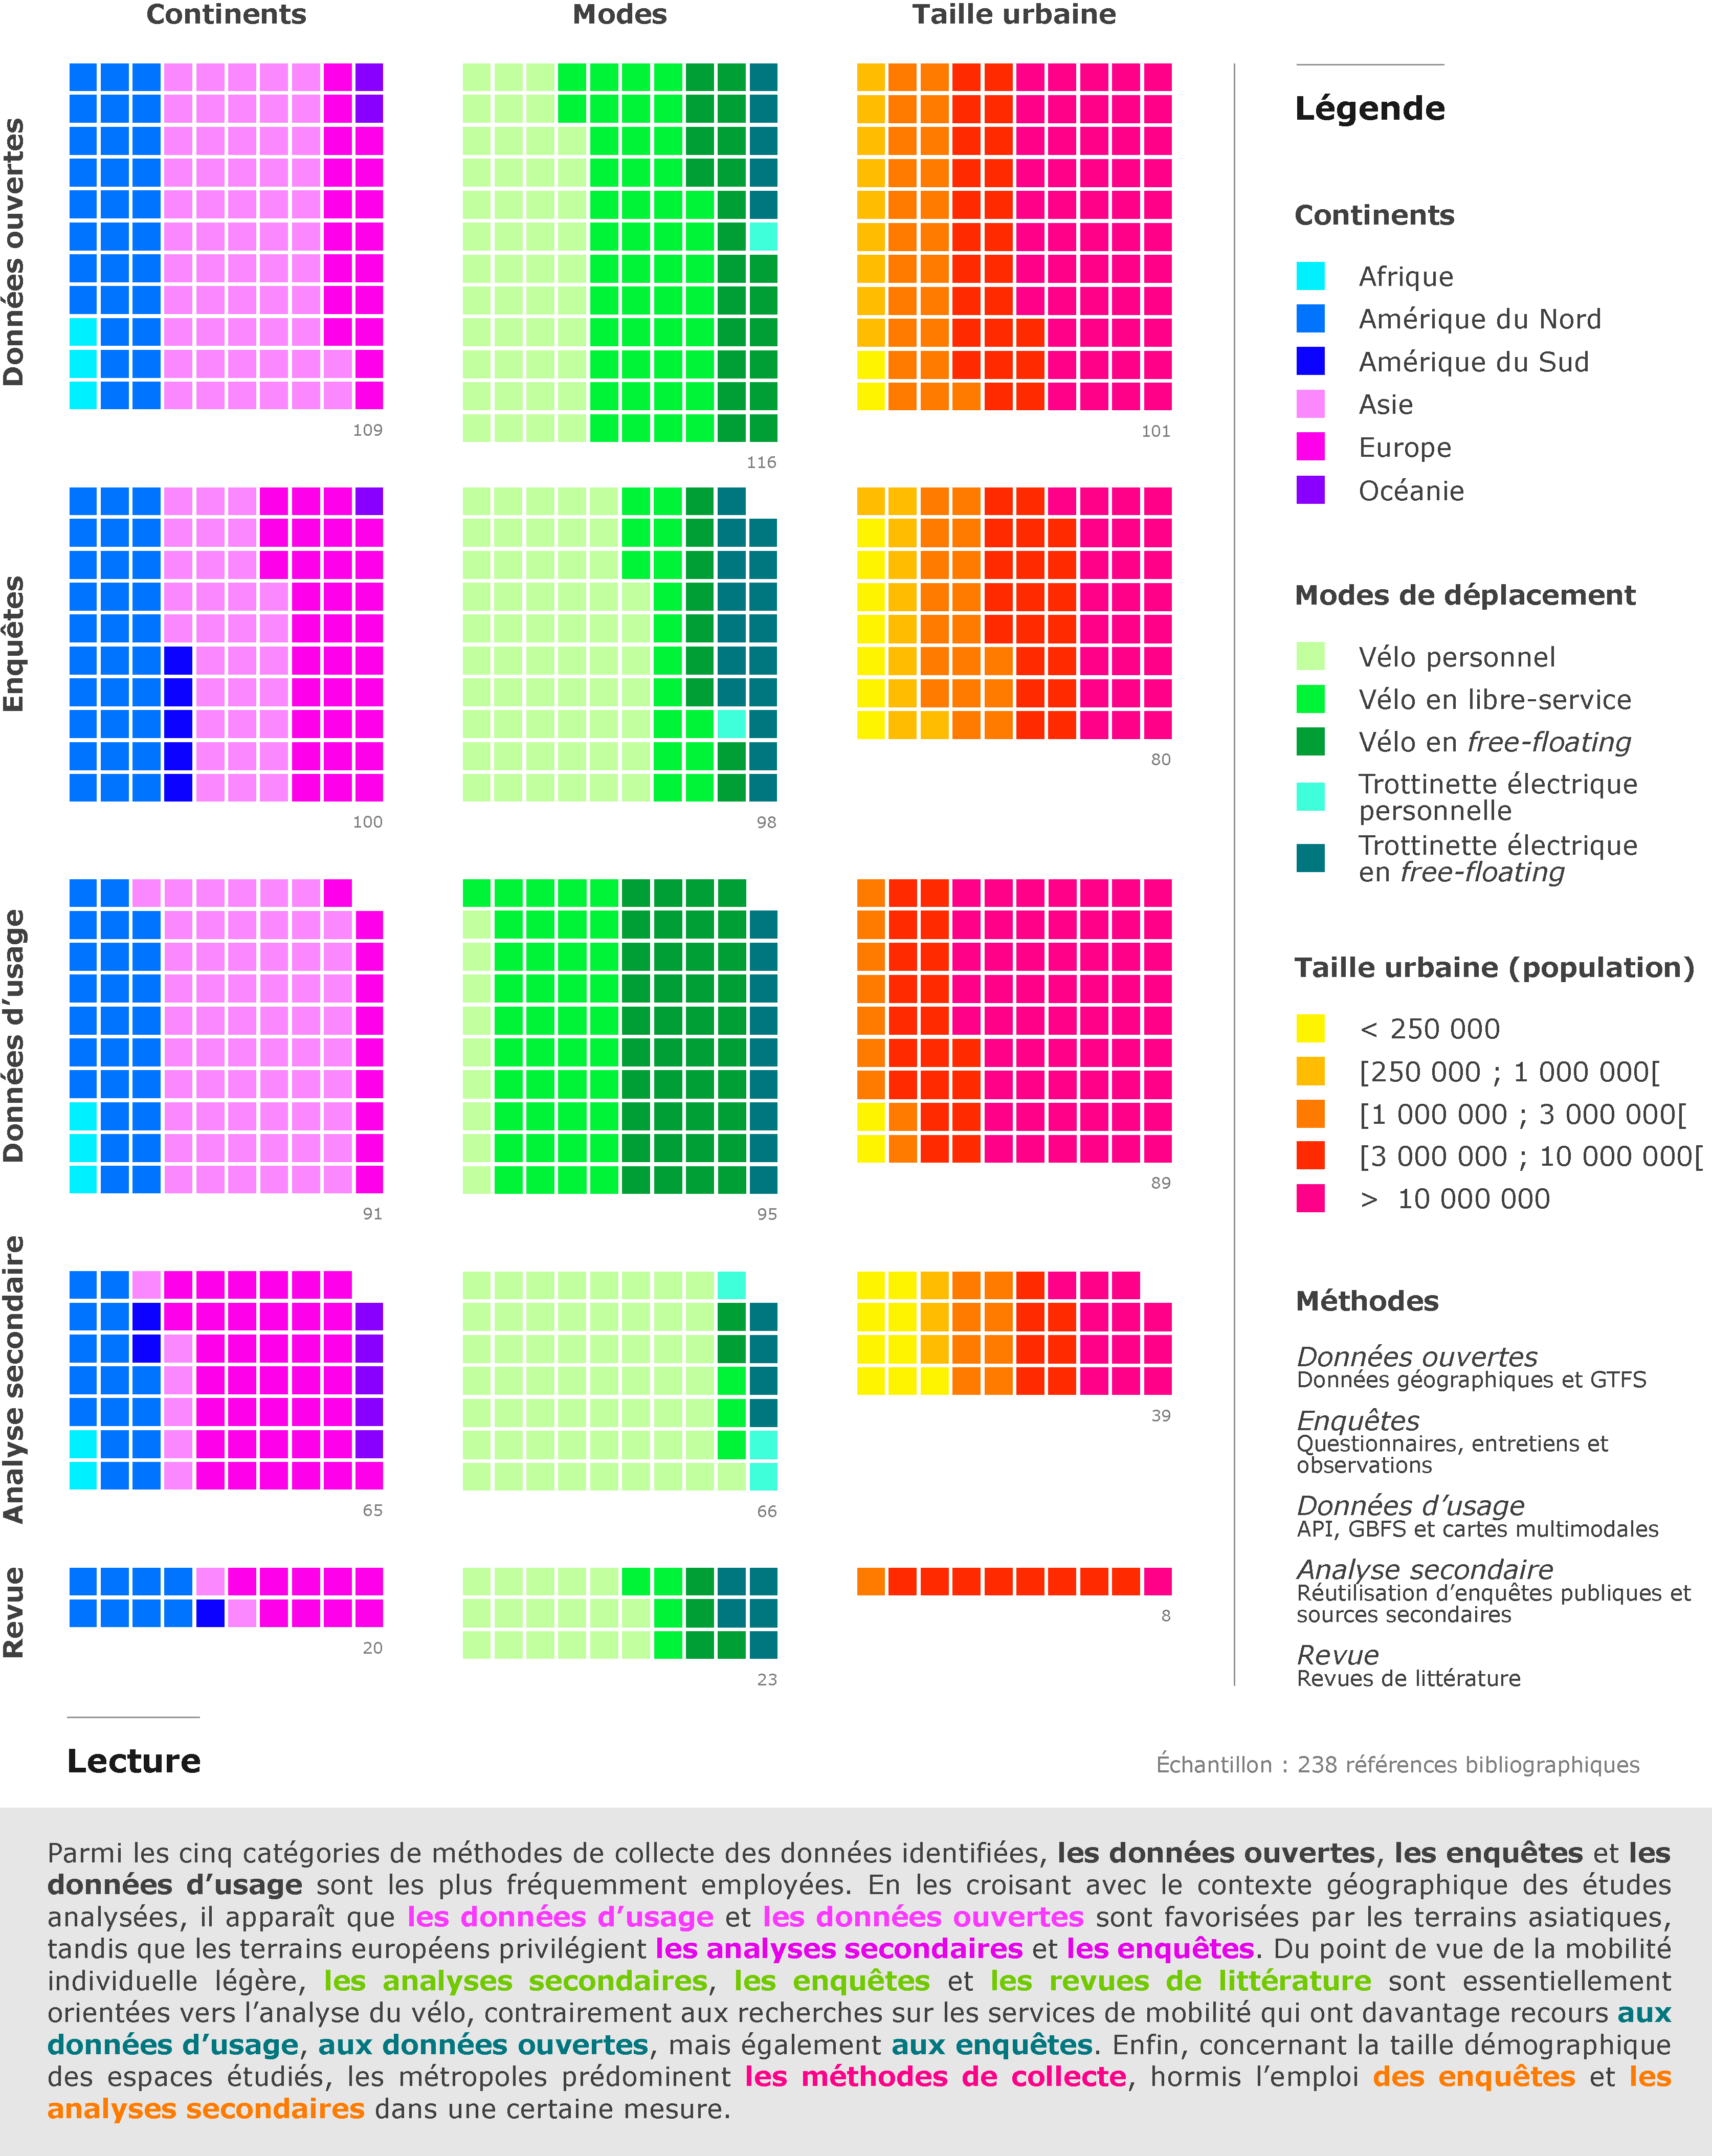
\includegraphics[width=1\columnwidth]{src/Figures/Chap-2/FR_RSL_Sources_donnees.pdf}}
        \vspace{5pt}
        \begin{flushright}\scriptsize{
        Auteur~: \textcolor{blue}{Dylan Moinse (2023)}
        %\\
        %Réalisation avec \Marque{Excel}~et sur \Marque{Illustrator}
        }\end{flushright}
    \end{figure}

    % Sources de données par taille d'agglomération
Dans une perspective plus large, cette exploration méthodologique révèle comment la taille urbaine est capable d'influencer des modalités d'investigation distinctes en matière d'accès empirique au terrain et aux informations. En posant un regard sur la typologie des intercommunalités, il devient possible de discerner des schémas évoquant certaines stratégies quant à l'exploitation des données disponibles sur les terrains d'étude. Ainsi, l'\hyperref[fig-chap2:sources-donnees-rsl]{illustration~\ref{fig-chap2:sources-donnees-rsl}} (page~\pageref{fig-chap2:sources-donnees-rsl}) met en lumière une surreprésentation des mégapoles au sein de la \textsl{Big Data}, avec une emphase particulière sur l'\acrshort{API} et le \acrshort{GBFS}. Cette prépondérance découle de la concentration d'offres de vélo et de micro-mobilité en libre-service, qu'elles soient dotées d'infrastructures de stationnement ou qu'elles fonctionnent sans celles-ci.  À l'inverse, les données mises à disposition concernant l'occupation des sols et les réseaux de transport en commun s'avère distribuées de manière plus équilibrée. En ce qui concerne la mise en œuvre d'enquêtes par voie de questionnaire, il est à noter que les métropoles comptant moins de trois millions d'habitant·e·s bénéficient davantage de l'usage du questionnaire en ligne. Les agglomérations d'au moins 250~000~habitant·e·s semblent plutôt s'orienter vers des questionnaires en face-à-face. Par ailleurs, l'analyse secondaire d'enquêtes publiques se révèle être une option privilégiée au sein d'une proportion significative d'agglomérations de taille démographique plus modeste. Cette lecture statistique peut s'expliquer par les différences de disponibilité en matière de ressources selon les spécificités des terrains géographiques. En effet, les données massives sur un territoire donné étant plus rarement constituées dans les territoires faiblement peuplés, les enquêtes permettent de pallier cette situation tout en étant plus abordables et moins chronographes.%%Rédigé%%

    % Sources de données par micro-mobilité
L'analyse des méthodes de collecte des données a été croisée avec les formes de mobilité individuelle légère telles qu'elles sont abordées dans le corpus scientifique. Si le vélo à usage personnel et en intermodalité est principalement conduit au moyen du questionnaire en face-à-face ou d'une analyse secondaire, l'étude du vélo et de la micro-mobilité partagés s'appuie sur l'exploitation de la \textsl{Big Data}. D'une part, l'examen du système de \acrshort{VLS} s'articule largement autour des données générées par le \acrshort{GBFS}. D'autre part, l'investigation des services de \acrshort{VFF} et de \acrshort{TEFF} se fonde principalement sur l'exploitation de l'\acrshort{API} (voir l'\hyperref[fig-chap2:sources-donnees-rsl]{illustration~\ref{fig-chap2:sources-donnees-rsl}}, page~\pageref{fig-chap2:sources-donnees-rsl}). Contrairement à la mobilité individuelle légère et partagée qui génère une grande quantité de données en temps réel, les données concernant le vélo à usage personnel étant plus difficilement accessibles sous forme de données massives, les recherches sur ce mode de déplacement individuel semblent se tourner vers des enquêtes préexistantes ou sur des enquêtes de terrain en interaction directe avec les usager·ère·s.%%Rédigé%%

    % Sources de données exemples questionnaire en face-à-face
En guise d'illustration, nous pouvons citer les recherches sur le vélo à usage personnel et employant le questionnaire en face-à-face de \textcolor{blue}{\textcite[1696]{cheng_evaluating_2012}}\index{Cheng, Yung-Hsiang|pagebf}\index{Liu, Kuo-Chu|pagebf} en association avec le métro à Kaohsiung (386 réponses), de \textcolor{blue}{\textcite[41]{jansson_almeida_alternativas_2022}}\index{Jansson Almeida, Bárbara|pagebf} avec le métro à Porto Alegre (212~réponses), de \textcolor{blue}{\textcite[183]{pan_intermodal_2010}}\index{Pan, Haixiao|pagebf}\index{Shen, Qing|pagebf}\index{Xue, Song|pagebf} sur le vélo et le \acrfull{VAE} avec le métro à Shanghai (600~réponses), de \textcolor{blue}{\textcite[7]{bauer_influence_2021}}\index{Bauer, Marek|pagebf}\index{Kisielewski, Piotr|pagebf} avec le train et le bus à Tarnow (501~réponses), de \textcolor{blue}{\textcite[685, 4]{rastogi_travel_2003, rastogi_willingness_2010}}\index{Rastogi, Rajat|pagebf}\index{Krishna Rao,~K.~V.|pagebf} sur la marche et le vélo avec le train à Mumbai (1~449 réponses), de \textcolor{blue}{\textcite[2]{rijsman_walking_2019}}\index{Rijsman, Lotte|pagebf}\index{Oort, Niels van|pagebf}\index{Ton, Danique|pagebf}\index{Hoogendoorn, Serge|pagebf}\index{Molin, Eric|pagebf}\index{Teijl, Thomas|pagebf} sur la marche et le vélo avec le tramway à La Haye (629 réponses) ou encore de \textcolor{blue}{\textcite[192]{sherwin_practices_2011}}\index{Sherwin, Henrietta|pagebf}\index{Parkhurst, Graham|pagebf}\index{Robbins, Derek|pagebf}\index{Walker, Ian|pagebf} qui mêlent le questionnaire et l'observation directe sur le vélo avec le train à Bristol (135 réponses).%%Rédigé%%

    % Sources de données exemples questionnaire en ligne
Des travaux menés à l'aide du questionnaire en ligne témoignent également d'une répartition déséquilibrée au profit du vélo à usage personnel, à l'instar des publications de \textcolor{blue}{\textcite[724]{waerden_relation_2018}}\index{Waerden, Peter|pagebf}\index{Waerden, Jaap|pagebf} sur la combinaison du vélo avec le train à Eindhoven (415 réponses), de \textcolor{blue}{\textcite[5, 488]{la_paix_puello_train_2016, la_paix_puello_role_2021}}\index{La Paix Puello, Lissy|pagebf}\index{Geurs, Karst~T.|pagebf} avec le train dans la région métropolitaine de Rotterdam-La Haye et dans la Randstad South (1~524 réponses), de \textcolor{blue}{\textcite[267]{krygsman_multimodal_2004}}\index{Krygsman, Stephan|pagebf}\index{Dijst, Martin|pagebf}\index{Arentze, Theo|pagebf} sur le vélo avec le train, le métro, le tramway et le bus dans la région métropolitaine d'Amsterdam-Utrecht
(1~966 ménages dont 755 cyclistes), de \textcolor{blue}{\textcite[663]{mil_insights_2020}}\index{Mil, Joeri~F.P. van|pagebf}\index{Leferink, Tessa~S.|pagebf}\index{Annema, Jan Anne|pagebf}\index{Oort, Niels van|pagebf} avec le train aux Pays-Bas (269 réponses), de \textcolor{blue}{\textcite[132-133]{chen_determinants_2012}}\index{Chen, Lijun|pagebf}\index{Pel, Adam~J.|pagebf}\index{Chen, Xuewu|pagebf}\index{Sparing, Daniel|pagebf}\index{Hansen, Ingo~A.|pagebf} avec le métro à Nanjing (1~784 réponses dont 136 cyclistes intermodaux·les), de \textcolor{blue}{\textcite[4259]{bopp_examining_2015}}\index{Bopp, Melissa|pagebf}\index{Gayah, Vikash~V.|pagebf}\index{Campbell, Matthew~E.|pagebf} sur la marche et le vélo avec le train, le métro et le tramway dans les États de Delaware, New Jersey, Maryland, Virginie-Occidentale, Pennsylvanie et de l'Ohio (1~234 réponses dont 152~voyageur·se·s), de \textcolor{blue}{\textcite[6]{jonkeren_bicycle-train_2021, jonkeren_bicycle_2021}}\index{Jonkeren, Olaf|pagebf}\index{Kager, Roland|pagebf}\index{Harms, Lucas|pagebf}\index{te Brömmelstroet, Marco|pagebf} sur l'usage et le stationnement des vélos à Rotterdam, Utrecht et Eindhoven ainsi qu'autour des gares néerlandaises (2~299 et 1~209 réponses dont 1~309 cyclistes intermodaux·les) ou encore de \textcolor{blue}{\textcite[6]{molin_bicycle_2015}}\index{Molin, Eric|pagebf}\index{Maat, Kees|pagebf} sur le stationnement vélo autour de la gare de Delft (866 réponses).%%Rédigé%%

    % Sources de données exemples analyse secondaire
La dichotomie entre les méthodes de collecte de données propres à ces modes de déplacement personnels et partagés est également visible dans les productions scientifiques de \textcolor{blue}{\textcite[87]{taylor_analysis_1996}}\index{Taylor, Dean|pagebf}\index{Mahmassani, Hani|pagebf} qui ont conduit un questionnaire par courrier pour évaluer l'usage du vélo en combinaison avec le bus dans l'État du Texas (814 réponses), de \textcolor{blue}{\textcite[10]{pages_nouveaux_2021}}\index{Pages, Thibaud|pagebf}\index{Lammoglia, Adrien|pagebf}\index{Josselin, Didier|pagebf} qui ont réalisé un questionnaire en ligne (280~réponses) mêlé à des entretiens sur l'usage intermodal de la trottinette électrique à usage personnel ou bien de \textcolor{blue}{\textcite[60]{rabaud_quand_2022}}\index{Rabaud, Mathieu|pagebf}\index{Richer, Cyprien|pagebf} qui ont exploité plus de 40~enquêtes de mobilité datant de 2015-2019 pour étudier cet \acrfull{EDPM} en intermodalité en France (364~usager·ère·s de la trottinette). À ce titre, la réutilisation de données primaires en provenance d'enquêtes publiques souligne la présence marquée du vélo et plus largement de la mobilité individuelle légère, d'après les études réalisées par \textcolor{blue}{\textcite[8-10]{shelat_analysing_2018}}\index{Shelat, Sanmay|pagebf}\index{Huisman, Raymond|pagebf}\index{Oort, Niels van|pagebf} sur le vélo avec le train aux Pays-Bas, à partir de l'enquête de mobilité nationale \acrfull{OViN} de 2010-2015 (environ 250~000~ménages dont 3~376 cyclistes), par \textcolor{blue}{\textcite[9]{luan_better_2020}}\index{Luan, Xin|pagebf}\index{Cheng, Lin|pagebf}\index{Song, Yan|pagebf}\index{Zhao, Jinbao|pagebf} sur le vélo avec le métro, à partir de l'enquête de mobilité nationale de Nanjing de 2014 (10~385 ménages dont 3~999 cyclistes), par \textcolor{blue}{\textcite[3]{zuo_determining_2018}}\index{Zuo, Ting|pagebf}\index{Wei, Hang|pagebf}\index{Rohne, Andrew|pagebf} sur le vélo avec le bus à Cincinnati, à partir de l'enquête de mobilité de l'Ohio de 2009-2010 (2~059 ménages) ou encore par \textcolor{blue}{\textcite[76]{oostendorp_combining_2018}}\index{Oostendorp, Rebekka|pagebf}\index{Gebhardt, Laura|pagebf} sur le vélo avec le train, le métro, le tramway et le bus à Berlin, à partir du recensement de la population de Berlin (1~098 individus dont 363 cyclistes intermodaux·les).%%Rédigé%%

    % 2.2.2.3. Types d’analyse
    \needspace{1\baselineskip} % Réserve de l'espace
\subsubsection*{Démarches et types d'analyse
    \label{chap2:demarches-types-analyses}
    }
    
    % Introduction
Dans le cadre de cette recherche doctorale, une analyse exhaustive des méthodes employées dans le corpus de la \acrshort{RSL} a été réalisée, révélant une diversité conséquente des techniques d'analyse catégorisées. Au total, 484 méthodes d'analyse ont été identifiées, correspondant à 273 approches distinctes. Parmi ces démarches, la modélisation se distingue comme l'outil analytique le plus fréquemment utilisé, avec 62~occurrences au sein du corpus. Cette méthode est suivie de près par l'utilisation du \acrfull{SIG}, recensée 51~fois. Les questionnaires sont également fréquemment utilisés, avec 30~mentions. Enfin, les revues de littérature, recensées 17 fois, soulignent l'importance de la synthèse des connaissances existantes. La diversité des techniques mises en évidence traduit un éventail d'approches, allant du quantitatif au qualitatif. Cette variété méthodologique permet d'aborder les problématiques de la mobilité urbaine sous des angles multiples, offrant une compréhension plus riche et nuancée des interactions entre la mobilité individuelle légère intégrée aux systèmes de transport en commun et les systèmes urbains.%%Rédigé%%

    % Statistiques descriptives (quantitatif)
En lien avec le sujet de recherche sur le \acrshort{M-TOD}, l'approche quantitative est la méthode d'analyse la plus sollicitée, avec une présence marquée de mesures descriptives au sein de 80~articles scientifiques et de la modélisation dans 62~études. D'une part, l'analyse statistique descriptive est relevée dans 50~publications, suivies respectivement des entretiens par questionnaire basés sur les préférences déclarées (\textsl{Stated Preference}, SP)\footnote{
    Le questionnaire par préférences déclarées est une technique de collecte de données où les répondant·e·s sont interrogé·e·s sur leurs préférences dans des scénarios hypothétiques, afin d'estimer la valeur attribuée à des biens, à des services ou à des changements d'usage.
} et les préférences révélées (\textsl{Revealed Preference}, RP)\footnote{
    Le questionnaire par préférences révélées est une technique de collecte de données basée sur l'observation des choix des individus dans des conditions réelles.
} dans 20~et~10~articles. D'autre part, les études faisant appel à la modélisation statistique embrassent une diversité d'approches. Nous comptons neuf recherches utilisant des modèles de prédiction de la demande (\textsl{Demand Forecasting Models}, DFM)\footnote{
    Le modèle de prédiction de la demande est un outil économétrique utilisé pour estimer la future demande d'un produit ou service, dépendante d'une multitude de variables comme le prix, le revenu ou les préférences des consommateur·rice·s.
}, quinze recourant au modèle de choix discrets (\textsl{Discrete Choice Models}, DCM)\footnote{
    Le modèle de choix discrets est un outil économétrique utilisé pour prédire les choix effectués par les individus parmi un ensemble fini d'options, en reposant sur la théorie de l'utilité aléatoire, où le choix d'un individu est modélisé comme une fonction de divers attributs des options disponibles.
}, dont sept appliquant le modèle logit multinomial (\textsl{Multinomial Logit Model}, MLN)\footnote{
    Le modèle logit multinomial est une extension du modèle logit binaire, utilisé pour modéliser les choix parmi plus de deux alternatives discrètes, généralement des modes de déplacement.
}, tandis que sept autres reposent sur le modèle de régression des moindres carrés ordinaires (\textsl{Ordinary Least Squares Regression}, OLS)\footnote{
    Le modèle de régression des moindres carrés est une méthode de régression linéaire qui minimise la somme des carrés des écarts entre les valeurs observées et celles estimées par le modèle.
}. Ces modèles de régression, fréquemment mobilisés, offrent une approche robuste pour l'analyse des relations entre variables. En complément, certaines études adoptent une approche par clustérisation, notamment la clustérisation k-means (\textsl{k-means clustering})\footnote{
    Les k-means sont une méthode de clustérisation destinée à diviser un ensemble de données en $ k $ groupes distincts, tout en minimisant la variance au sein du cluster et en maximisant la variance entre les classes.
}, présente dans sept articles. Enfin, l'\acrfull{ACB}\footnote{
    L'analyse coût-bénéfice sert à évaluer les avantages attends et les coûts associés d'un projet dans le but de déterminer sa viabilité et les meilleures options.
} est présente dans trois publications, tandis que les modèles de trafic sont mentionnés dans deux études.%%Rédigé%%
    
    % Cartographie (SIG)
L'application des méthodes relatives à la science des données quantitatives (\textsl{Data Science}), se manifeste également au travers de l'approche géostatistique. Cette dernière s'appuie en particulier sur l'usage du \acrshort{SIG}, un outil d'analyse spatiale intégré dans 51~documents étudiés dans le corpus. En parallèle de l'utilisation directe du \acrshort{SIG}, diverses techniques complémentaires d'analyse spatiale sont mises en œuvre. Parmi ces méthodes, on retrouve notamment la régression géographique pondérée (\textsl{Geographically Weighted Regression}, GWR)\footnote{
    La régression géographique pondérée est une technique de modélisation spatiale qui permet d'analyser la variation spatiale dans les relations entre les variables, en attribuant un poids différent à chaque observation en fonction de son emplacement.
}, employée dans neuf études. Huit études intègrent l'autocorrélation spatiale\footnote{
    L'autocorrélation spatiale se mesure notamment à l'aide de l'indice de Moran. Cet indice est utilisé en géostatistique pour évaluer si un modèle présente des motifs spatiaux aléatoires, regroupés ou dispersés. Un indice de Moran proche de +1 indique une forte corrélation spatiale positive, tandis qu'un indice proche de -1 indique une forte corrélation spatiale négative.
}, tandis que la mesure de l'indice de connectivité des réseaux (\textsl{Network Connectivity Index}, NCI)\footnote{
    L'indice de connectivité des réseaux est une mesure quantitative utilisée pour évaluer le degré de connectivité au sein d'un réseau de transport en commun ou de communication, en considérant le nombre de liens, la directivité des connexions et la distance entre chaque nœud.
}, quant à elle, est exploitée dans sept études. Deux travaux se distinguent par la détermination de l'indice nœud-lieu (\textsl{Node-Place Index})\footnote{
    L'indice nœud-lieu est un outil d'analyse spatiale utilisé pour évaluer la fonctionnalité des nœuds de transport dans leur contexte urbain, en combinant des aspects relatifs au transport et à l'urbanisme, de sorte à évaluer les interactions entre les stations de transport en commun et l'environnement urbain.
}. Enfin, l'estimation de la densité du noyau (\textsl{Kernel Density Estimation}) est appliquée dans une étude, de même que le diagramme de Voronoï\footnote{
    Le diagramme de Voronoï est une partition en cellules d'un ensemble spécifique de points sur un plan Euclidien. Chaque point génère une région cellulaire contenant tous les points du plan plus proches de ce point que de tout autre.
}. Ces approches diversifiées démontrent la richesse et la complexité des analyses spatiales dans l'étude du \acrshort{M-TOD} qui sont alors enrichies par des approches qualitatives.%%Rédigé%%

    % Discours (qualitatif)
L'approche méthodologique qualitative est circonscrite à un corpus de onze publications. Parmi celles-ci, neuf se fondent principalement sur l'analyse discursive, menée à l'aide d'entretiens semi-directifs, alors que les deux autres se distinguent par une exploration sensible de l'environnement urbain et des interactions sociales. Toutefois, l'approche qualitative peut également être étendue aux dix-sept revues de littérature synthétisant indirectement le sujet de recherche relatif au \acrshort{M-TOD}. Ces méthodes proviennent d'une variété de domaines de connaissancere, allant de l'économie, avec des approches telles que l'économétrie (DCM et MLN) et l'économie des transports (SP, RP, DFM et modèles de transport)~; à la statistique, incluant les sciences de la donnée et les k-means. Elles englobent également la géographie, avec l'analyse spatiale (diagramme de Voronoï et GWR)~; et touchent à la sociologie, notamment à travers les entretiens.%%Rédigé%%

    % ___________________________________________
    % 2.3.
    \newpage
    \needspace{1\baselineskip} % Réserve de l'espace
    \sectionheader{État des connaissances actuelles sur le M-TOD}
\section{Caractérisation d'un \textsl{Micromobility-friendly Transit-Oriented Development} au prisme des caractéristiques de l'environnement urbain et des choix individuels
    \label{chap2:caracterisation-btod-environnement-urbain-choix-individuels}
    }
    
    % Introduction 1
La section actuelle de ce chapitre est consacrée à une étude détaillée visant à définir les attributs fondamentaux du \acrshort{M-TOD}, en le réfléchissant au prisme de l'environnement urbain ainsi que des préférences personnelles en matière de mobilité. Dans cette optique, nous avons opté pour une démarche inductive structurée autour des \Guillemets{\acrshort{7Ds}}~enrichie par des variables additionnelles en lien avec les pratiques intermodales examinées. L'objectif de cette analyse issue de la \acrshort{RSL} est de cerner les contours du modèle urbain du \acrshort{M-TOD}, en s'appuyant sur une mise en perspective des études empiriques internationales. Il s'agit de déceler les caractéristiques récurrentes émanant de cette revue de littérature. Par conséquent, notre ambition est également de saisir la façon dont le \acrshort{M-TOD} peut être envisagé comme un complément au \acrshort{TOD} et d'appréhender dans quelle mesure les dimensions analysées de ce concept d'urbanisme se reflètent dans une stratégie urbaine qui intègre la mobilité individuelle légère.%%Rédigé%%

    % Introduction 2
Au travers de leur \acrshort{RSL}, \textcolor{blue}{\textcite[294]{zhang_built_2023}}\index{Zhang, Yushan|pagebf}\index{Kasraian, Dena|pagebf}\index{Wesemael, Pieter van|pagebf} dévoilent à quel point les études portant sur le vélo et la micro-mobilité se focalisent spécifiquement sur les stratégies de gestion et d'exploitation de ces modes de déplacement, de même que sur l'analyse des profils et des comportements des usager·ère·s. Toutefois, une attention moindre a été accordée à l'interrelation de la mobilité individuelle légère avec l'environnement urbain. De ce fait, le présent chapitre s'attache principalement à explorer cet aspect essentiel, mais jusqu'alors sous-examiné, qui est crucial dans la conceptualisation du \acrshort{M-TOD}. Conformément à la définition établie par \textcolor{blue}{\textcite[65]{handy_how_2002}}\index{Handy, Susan~L.|pagebf}\index{Boarnet, Marlon~G.|pagebf}\index{Ewing, Reid|pagebf}\index{Killingsworth, Richard~E.|pagebf}, l'environnement urbain se distingue par trois composantes majeures~: (i) le \textsl{design} urbain, englobant la configuration des espaces publics~; (ii) l'utilisation des sols, se rapportant à la localisation, la répartition et la densité des activités dans l'espace~; et (iii) le système de mobilité, comprenant tant l'infrastructure de transport que le niveau de service des réseaux (\textsl{Level of Service}, LoS). C'est sur ces fondements conceptuels que s'appuie notre analyse des données collectées, aboutissant à un tableau synthétique où chaque étude a été évaluée au regard de la présence ou de l'absence de ces dimensions (voir l'\hyperref[annexes:rsl-resultats]{annexe~\ref{annexes:rsl-resultats}}, page~\pageref{annexes:rsl-resultats}).%%Rédigé%%

    % Annonce du plan
Cette section s'efforcera alors de caractériser le \acrshort{M-TOD}, dans l'intention de présenter une définition de ce modèle urbain fondée sur les connaissances issues de la littérature scientifique. Divers aspects seront traités, à commencer par les \Guillemets{\acrshort{7Ds}}, soit la \hyperref[chap2:densite-population]{densité de population (\(D1\))} (page~\pageref{chap2:densite-population}), la \hyperref[chap2:diversite-fonctionnelle]{diversité d'usage des sols (\(D2\))} (page~\pageref{chap2:diversite-fonctionnelle}), la \hyperref[chap2:traitement-espaces-publics]{conception des espaces publics (\(D3\))} (page~\pageref{chap2:traitement-espaces-publics}), l'\hyperref[chap2:accessibilite-intermodale]{accessibilité vers les ressources territoriales (\(D4\))} (page~\pageref{chap2:accessibilite-intermodale}), la \hyperref[chap2:distances-premiers-derniers-km]{taille des quartiers de gare (\(D5\))} (page~\pageref{chap2:distances-premiers-derniers-km}), la \hyperref[chap2:gestion-demande-mobilite]{gestion de la demande de mobilité (\(D6\))} (page~\pageref{chap2:gestion-demande-mobilite}), la \hyperref[chap2:sociodemographie-usagers]{dimension liée à l'inclusion sociale (\(D7\))} (page~\pageref{chap2:sociodemographie-usagers}), suivis des \hyperref[chap2:comportements-mobilite]{comportements de mobilité} (page~\pageref{chap2:comportements-mobilite}) et des \hyperref[chap2:impacts-systemes-urbain-mobilite]{divers impacts} (page~\pageref{chap2:impacts-systemes-urbain-mobilite}).%%Rédigé%%

    % 2.3.1. Resultats~: densité
    \needspace{1\baselineskip} % Réserve de l'espace
\subsection{Densité de population
    \label{chap2:densite-population}
    }
    
    % Introduction
La première thématique abordée dans cette section est celle de la densité de population, un élément crucial pour le \acrshort{TOD}, en soutenant l'aménagement de territoires compacts et favorables aux piéton·ne·s. Présente dans 44 des 238 publications scientifiques examinées, la densité démographique influence positivement l'usage conjoint des transports en commun et de la mobilité individuelle légère.%%Rédigé%%

    % 2.3.1.1. Impact positif densité population
    \needspace{1\baselineskip} % Réserve de l'espace
\subsubsection*{Association positive avec la densité de population
    \label{chap2:association-positive-densite-population}
    }
    
    % Impact positif densité population avec vélo personnel
Au sein du corpus d'études examiné, une proportion significative de travaux suggère l'existence d'une corrélation positive entre la densité de population et l'interaction entre les systèmes de transport en commun et la mobilité individuelle légère. Ces recherches académiques mettent en évidence que les zones caractérisées par une densité démographique accrue tendent à enregistrer une utilisation plus intensive du vélo et de la micro-mobilité, en complémentarité avec les réseaux de transport en commun. Dans ce contexte, la densité de population se révèle être une dimension prépondérante, avec une relation positive établie entre ce facteur et la probabilité d'utiliser le vélo en association avec le train et le bus, au Danemark \textcolor{blue}{\autocite[41]{nielsen_bikeability_2018}}\index{Nielsen, Thomas Alexander Sick|pagebf}\index{Skov-Petersen, Hans|pagebf}. De manière similaire, aux États-Unis, la part modale du vélo en combinaison avec le train et le bus a connu une augmentation notable dans les régions à forte densité de population \textcolor{blue}{\autocite[107]{wang_bicycle-transit_2013}}\index{Wang, Rui|pagebf}\index{Liu, Chen|pagebf}. \textcolor{blue}{\textcite[212]{kager_characterisation_2016}}\index{Kager, Roland|pagebf}\index{Bertolini, Luca|pagebf}\index{te Brömmelstroet, Marco|pagebf} affirment que le vélo complète efficacement le train dans des milieux denses, mais aussi en s'adaptant à des densités moins élevées dans divers contextes, notamment à Amsterdam, Amstelveen, Diemen et Ouder-Amstel. À Amsterdam, \textcolor{blue}{\textcite[344]{kampen_bicycle_2021}}\index{Kampen, Jullian van|pagebf}\index{Pauwels, Eric|pagebf}\index{Mei, Rob van der|pagebf}\index{Dugundji, Elenna~R.|pagebf} ont constaté que la densité du bâti joue un rôle crucial dans le choix des emplacements de stationnement de vélos personnels, les quartiers à forte densité urbaine attirant davantage de stationnements de vélos près des gares et des stations de métro.%%Rédigé%%

    % Impact positif densité population avec le VLS
Dans une perspective similaire concernant le vélopartage, un lien positif est suggéré entre la densité de population et l'utilisation du \acrshort{VLS} en synergie avec le réseau ferroviaire, comme observé à Chicago, New York City et Washington~D.C. \textcolor{blue}{\autocite[16]{kong_deciphering_2020}}\index{Kong, Hui|pagebf}\index{Jin, Scarlett~T.|pagebf}\index{Sui, Daniel~Z.|pagebf}. Cette interrelation est également confirmée entre le \acrshort{VLS} et le métro, tant à Beijing \textcolor{blue}{\autocite[9]{yu_understanding_2021}}\index{Yu, Senbin|pagebf}\index{Liu, Gehui|pagebf}\index{Yin, Congru|pagebf}, qu'à Nanjing \textcolor{blue}{\autocite[12]{chen_what_2022}}\index{Chen, Wendong|pagebf}\index{Chen, Xuewu|pagebf}\index{Chen, Jingxu|pagebf}\index{Cheng, Long|pagebf}. \textcolor{blue}{\textcite[15]{li_investigating_2022}}\index{Li, Xiaofeng|pagebf}\index{Wu, Yao-Jan|pagebf}\index{Khani, Alireza|pagebf} avancent que dans les zones à forte densité démographique, une interaction positive est manifeste entre le \acrshort{VLS} et le tramway ainsi que le bus, à Tucson. À Oslo, \textcolor{blue}{\textcite[399]{bocker_bike_2020}}\index{Böcker, Lars|pagebf}\index{Anderson, Ellinor|pagebf}\index{Uteng, Tanu Priya|pagebf}\index{Throndsen, Torstein|pagebf} soulignent que l'usage fréquent du \acrshort{VLS} en association avec le métro est prédominant dans les territoires densément peuplés.%%Rédigé%%

    % Impact positif densité population avec le VFF
Plusieurs études menées à Shenzhen et Shanghai, respectivement par \textcolor{blue}{\textcite[6]{wang_relationship_2020}}\index{Wang, Ruoyu|pagebf}\index{Lu, Yi|pagebf}\index{Wu, Xueying|pagebf}\index{Liu, Ye|pagebf}\index{Yao, Yao|pagebf} et \textcolor{blue}{\textcite[31]{lin_analysis_2019}}\index{Lin, Diao|pagebf}\index{Zhang, Yongping|pagebf}\index{Zhu, Ruoxin|pagebf}\index{Meng, Liqiu|pagebf}, corroborent que les densités élevées de population sont positivement associées à l'usage du \acrshort{VFF} avec le métro, révélant une demande accrue dans les zones urbaines denses. \textcolor{blue}{\textcite[16]{li_operating_2019}}\index{Li, Yuan|pagebf}\index{Zhu, Zhenjun|pagebf}\index{Guo, Xiucheng|pagebf} ont mis en évidence, à travers une classification des stations de métro, que celles situées dans les quartiers densément peuplés du centre urbain de Nanjing connaissent un usage plus important du \acrshort{VFF} pour les \Guillemets{premiers et derniers kilomètres}. Les travaux menés par \textcolor{blue}{\textcite[25]{guo_dockless_2021}}\index{Guo, Yuanyuan|pagebf}\index{Yang, Linchuan|pagebf}\index{Lu, Yi|pagebf}\index{Zhao, Rui|pagebf} et par \textcolor{blue}{\textcite[184]{cheng_exploring_2022}}\index{Cheng, Long|pagebf}\index{Wang, Kailai|pagebf}\index{Vos, Jonas de|pagebf}\index{Huang, Jie|pagebf}\index{Witlox, Frank|pagebf} démontrent que la densité démographique est significativement liée à l'utilisation intégrée du \acrshort{VFF} avec le métro pendant les heures de pointe, respectivement à Shenzhen et Nanjing. À Suzhou, \textcolor{blue}{\textcite[24]{li_integration_2020}}\index{Li, Jie|pagebf}\index{Lu, Yang|pagebf}\index{Ling, Lei|pagebf} observent qu'une densité de population plus élevée diminue la probabilité de choisir le bus au profit du \acrshort{VFF} pour rejoindre les stations de métro. À Beijing, \textcolor{blue}{\textcite[11]{liu_temporal_2022}}\index{Liu, Siyang|pagebf}\index{Zhang, Xiaodong|pagebf}\index{Zhou, Chenjing|pagebf}\index{Rong, Jian|pagebf}\index{Bian, Yang|pagebf} révèlent qu'une augmentation de 10~\% de la densité entraîne une hausse significative de l'utilisation du \acrshort{VFF} avec le métro durant les jours de semaine, et plus encore durant les heures de pointe matinales. Une conclusion similaire émerge dans le cas de la \acrshort{TEFF} avec le métro, où une concentration a été identifiée dans des zones densément peuplées à New York City \textcolor{blue}{\autocite[16]{lee_forecasting_2021}}\index{Lee, Mina|pagebf}\index{Chow, Joseph|pagebf}\index{Yoon, Gyugeun|pagebf}\index{He, Brian|pagebf}.%%Rédigé%%

    % Impact positif densité population avec les TC
L'analyse de la \acrshort{RSL} tend également à souligner une amplification de l'utilisation des transports en commun, en questionnant les liens entre la densité démographique et l'usage intermodal de la mobilité individuelle légère. Les zones à forte densité favorisent ainsi l'usage du transport public en attirant un nombre croissant de passager·ère·s qui adoptent le vélo et la micro-mobilité. Dans les quartiers résidentiels des Pays-Bas, la densité de population s'avère être un facteur déterminant qui influence significativement l'usage des transports en commun, incluant le train, le métro, le tramway, le bus et même le ferry, par les cyclistes \textcolor{blue}{\autocite[334]{martens_promoting_2007}}\index{Martens, Karel|pagebf}. À Shanghai, la recherche conduite par \textcolor{blue}{\textcite[10]{li_exploring_2021}}\index{Li, Wenxiang|pagebf}\index{Chen, Shawen|pagebf}\index{Dong, Jieshuang|pagebf}\index{Wu, Jingxian|pagebf} indique que la densité démographique est positivement corrélée avec la distance de transfert, tant en \gls{rabattement} qu'en \gls{diffusion}, ce qui suggère que les stations de métro attirent des usager·ère·s du \acrshort{VFF} plus éloigné·e·s. En outre, lors de l'étape de post-acheminement à partir des stations de métro, la densité de population à Kaohsiung stimule considérablement l'intention des passager·ère·s d'avoir recours au \acrshort{VLS} \textcolor{blue}{\autocite[29]{cheng_expanding_2018}}\index{Cheng, Yung-Hsiang|pagebf}\index{Li, Yi-Chun|pagebf}.%%Rédigé%%

    % 2.3.1.2. Impact complexe densité population
    \needspace{1\baselineskip} % Réserve de l'espace
\subsubsection*{Relations complexes avec la densité de population
    \label{chap2:relations-complexes-densite-population}
    }
    
    % Relation complexe densité et intermodalité
L'examen de la relation entre la densité démographique et l'usage intermodal du vélo et de la micro-mobilité révèle une complexité accrue au sein d'une partie du corpus étudié, certaines recherches mettant en lumière une corrélation plus nuancée, voire ambigüe, entre ces différentes variables. Diverses études suggèrent que la densité de population ne constitue pas un facteur déterminant dans l'utilisation conjointe de la mobilité individuelle légère, notamment en ce qui concerne le vélo et le train à Melbourne \textcolor{blue}{\autocite[403]{weliwitiya_bicycle_2019}}\index{Weliwitiya, Hesara|pagebf}\index{Rose, Geoff|pagebf}\index{Johnson, Marilyn|pagebf}, le \acrshort{VLS} et le bus à Birmingham \textcolor{blue}{\autocite[5]{glass_role_2020}}\index{Glass, Caroline|pagebf}\index{Appiah-Opoku, Seth|pagebf}\index{Weber, Joe|pagebf}\index{Jones, Steven~L.|pagebf}\index{Chan, Amber|pagebf}\index{Oppong, Judith|pagebf}, ou encore le \acrshort{VFF} et le métro à Shenzhen \textcolor{blue}{\autocites[11]{guo_built_2020}[388]{guo_role_2021}}\index{Guo, Yuanyuan|pagebf}\index{He, Sylvia~Y.|pagebf}. À Utrecht, \textcolor{blue}{\textcite[274]{krygsman_multimodal_2004}}\index{Krygsman, Stephan|pagebf}\index{Dijst, Martin|pagebf}\index{Arentze, Theo|pagebf} ont démontré l'existence d'une relation non linéaire entre la densité de population et le choix du vélo, en particulier aux abords des gares et des stations de métro, de tramway et de bus, où une densité urbaine plus marquée favorise des distances plus courtes, propices à la marche. Une densité de population plus importante à Beijing n'entrainerait pas d'effet notable sur l'usage du \acrshort{VLS}, contrairement à une utilisation accrue des taxis, en particulier par les usagères, pour rejoindre le métro \textcolor{blue}{\autocite[15]{ni_exploring_2020}}\index{Ni, Ying|pagebf}\index{Chen, Jiaqi|pagebf}. À Beijing, l'utilisation du VLS en combinaison avec le métro s'accroît avec la densité de population, mais cette corrélation n'est pas constatée dans les modèles appliqués à Taipei et Tokyo \textcolor{blue}{\autocite[216]{lin_built_2018}}\index{Lin, Jen-Jia|pagebf}\index{Zhao, Pengjun|pagebf}\index{Takada, Kazuyuki|pagebf}\index{Li, Shengxiao|pagebf}\index{Yai, Tetsuo|pagebf}\index{Chen, Chi-Hao|pagebf}. Dans un contexte similaire, \textcolor{blue}{\textcite[45]{la_paix_puello_modelling_2015}}\index{La Paix Puello, Lissy|pagebf}\index{Geurs, Karst~T.|pagebf} ont noté qu'une densité élevée semble décourager l'utilisation du vélo pour se rendre aux gares dans la région de Randstad South. De manière analogue, une densité de population significative près des stations de métro à Nanjing semble privilégier la marche comme mode d'accès au réseau ferré, au détriment du \acrshort{VLS} \textcolor{blue}{\autocite[17]{ji_public_2017}}\index{Ji, Yanjie|pagebf}\index{Fan, Yingling|pagebf}\index{Ermagun, Alizera|pagebf}\index{Cao, Xuening|pagebf}\index{Wang, Wei|pagebf}\index{Das, Kirti|pagebf}. \textcolor{blue}{\textcite[181]{gan_associations_2021}}\index{Gan, Zuoxian|pagebf}\index{Yang, Min|pagebf}\index{Zeng, Qingcheng|pagebf}\index{Timmermans, Harry~J.~P.|pagebf} révèlent qu'une augmentation de 1~\% de la densité de population augmente la probabilité de choisir la marche de 0,22~\% en pré-acheminement et de 0,36~\% en post-acheminement à partir d'une station de métro, à Nanjing. Dans une étude de cas spécifique du quartier de la gare de Mouans-Sartoux, \textcolor{blue}{\textcite[189]{moinse_intermodal_2022}}\index{Moinse, Dylan|pagebf}\index{Goudeau, Matthieu|pagebf}\index{L'Hostis, Alain|pagebf}\index{Leysens, Thomas|pagebf} ont observé que les voyageur·se·s en \acrshort{TEP} débutent et terminent plus fréquemment leur \gls{déplacement} intermodal dans des zones denses, contrairement aux voyageur·se·s à vélo personnel.%%Rédigé%%

    % Raisons
L'inclinaison en faveur d'une densification des territoires peut ainsi s'expliquer par l'amélioration de l'accessibilité et une demande renforcée en termes de mobilité grâce à la concentration des populations. La corrélation positive entre la densité démographique et une utilisation accrue de la mobilité individuelle légère en coordination avec les transports en commun pourrait également être due aux coûts additionnels liés à l'usage de l'automobile dans les zones densément peuplées, ce qui confère au vélo une attractivité plus marquée aux abords des quartiers de gare, comme le soulignent \textcolor{blue}{\textcite[751]{midenet_modal_2018}}\index{Midenet, Sophie|pagebf}\index{Côme, Etienne|pagebf}\index{Papon, Francis|pagebf} pour le cas d'Amboise. \textcolor{blue}{\textcite[11]{hu_examining_2022}}\index{Hu, Songhua|pagebf}\index{Chen, Mingyang|pagebf}\index{Jiang, Yuan|pagebf}\index{Sun, Wei|pagebf}\index{Xiong, Chenfeng|pagebf} rendent compte que la densité est intimement liée à l'offre en transport en commun à Shanghai~: les zones à forte densité de population près du centre-ville présentent moins d'activités de \acrshort{VFF} avec le métro par rapport aux zones périphériques urbaines. Dans le contexte de Nanjing, \textcolor{blue}{\textcite[9]{cheng_promoting_2022}}\index{Cheng, Long|pagebf}\index{Jin, Tanhua|pagebf}\index{Wang, Kailai|pagebf}\index{Lee, Yongsung|pagebf}\index{Witlox, Frank|pagebf} et \textcolor{blue}{\textcite[8]{cheng_comparison_2023}}\index{Cheng, Long|pagebf}\index{Huang, Jie|pagebf}\index{Jin, Tanhua|pagebf}\index{Chen, Wendong|pagebf}\index{Li, Aoyong|pagebf}\index{Witlox, Frank|pagebf} constatent que le \acrshort{VFF} en combinaison avec le métro est favorisé lorsque la densité de population est élevée, mais cette tendance s'inverse lorsque la densité atteint un seuil entre 18~000~et~23~000~habitant·e·s/km², au-delà duquel les effets deviennent incertains, probablement en raison de la congestion urbaine, de la pollution et des risques liés à la sécurité. \textcolor{blue}{\textcite[8]{zhou_spatially_2023}}\index{Zhou, Xiao|pagebf}\index{Dong, Quanhua|pagebf}\index{Huang, Zhou|pagebf}\index{Yin, Ganmin|pagebf}\index{Zhou, Guoqing|pagebf}\index{Liu, Yu|pagebf} parviennent à une conclusion similaire, mettant en évidence une relation non significative entre la densité et l'utilisation conjointe du \acrshort{VFF} avec le métro et le bus à Beijing, en raison de rues fréquentées et d'un trafic plus dense dans les zones à forte densité. Selon \textcolor{blue}{\textcite[3]{romm_differences_2022}}\index{Romm, Daniel|pagebf}\index{Verma, Priyanka|pagebf}\index{Karpinski, Elizabeth|pagebf}\index{Sanders, Tracy~L.|pagebf}\index{McKenzie, Grant|pagebf}, le vélo est plus fréquemment utilisé lors des \Guillemets{premiers kilomètres}~dans les quartiers densément peuplés du centre urbain de Boston, en raison de la possession moindre de véhicules motorisés par les résidents.%%Rédigé%%

    % Conclusion Densité
L'association existante entre la densité démographique et l'emploi de la mobilité individuelle légère, en synergie avec les systèmes de transport en commun, dans le cadre théorique du \acrshort{M-TOD}, révèle une certaine complexité. D'une part, un ensemble de recherches empiriques atteste d'une liaison positive entre ces facteurs, corroborant le rôle clé de la densité appliquée à l'aire secondaire du \acrshort{TOD}. D'autre part, une exploration approfondie de la littérature scientifique révèle une série de constatations parfois contradictoires quant à l'influence manifeste de la densité de population. Dans le sillage de cette analyse de la littérature scientifique consacrée à la place de ce paramètre territorial dans l'architecture du \acrshort{TOD}, il apparaît judicieux de formuler une approche nuancée. Entre autres, la documentation étudiée soulignerait une association, certes empreinte de complexité, mais vérifiée, entre la densité de population et l'intégration du vélo et de la micro-mobilité avec le transport public. Cette relation s'avère toutefois tributaire d'un éventail de facteurs liés aux caractéristiques propres de chaque système urbain.%%Rédigé%%

    % 2.3.2. Resultats~: diversité
    \needspace{1\baselineskip} % Réserve de l'espace
\subsection{Diversité fonctionnelle
    \label{chap2:diversite-fonctionnelle}
    }
    
    % Introduction
La diversité occupe une place prééminente dans la planification urbaine du \acrshort{M-TOD}, se manifestant principalement à travers la densité des emplois, la multiplicité des fonctions urbaines et la diversité socio-économique. Ces aspects ont été mis en exergue dans 36 des études constituant le corpus de la \acrshort{RSL}. Une attention particulière a été portée à la diversité des usages, considérée comme un levier favorable à l'intégration de la mobilité individuelle légère aux réseaux de transport en commun et à l'animation des territoires. L'importance de regrouper et de concentrer dans un même espace des lieux résidentiels, commerciaux, des bureaux et des espaces verts est reconnue. Toutefois, la question de la diversité des groupes sociaux, notamment à travers une offre de logements variée et abordable, reste sous-représentée dans les études se rapportant aux quartiers de gare étendus.%%Rédigé%%

    % 2.3.2.1. Densité d'emploi
    \needspace{1\baselineskip} % Réserve de l'espace
\subsubsection*{Densité d'emploi
    \label{chap2:densite-emplois}
    }
    
    % Impact positif de la densité d'emploi
Selon une majorité des travaux scientifiques analysés, il ressort que la densité d'emploi dans les quartiers avoisinant les gares, particulièrement les gares desservant les lieux d'activité, soutient de manière significative l'intégration de la mobilité individuelle légère avec les systèmes de transport en commun. En ce qui concerne l'utilisation intermodale du vélo personnel, \textcolor{blue}{\textcite[12]{zuo_promote_2020}}\index{Zuo, Ting|pagebf}\index{Wei, Heng|pagebf}\index{Chen, Na|pagebf} notent qu'une augmentation des emplois à proximité des arrêts de bus à Hamilton entraîne une fréquentation accrue de cyclistes. De même, \textcolor{blue}{\textcite[41]{nielsen_bikeability_2018}}\index{Nielsen, Thomas Alexander Sick|pagebf}\index{Skov-Petersen, Hans|pagebf} soulignent qu'une concentration d'emplois dans le secteur du détail au Danemark est fortement corrélée avec l'usage combiné du vélo, lorsqu'il est stationné à la gare d'origine, et du train. La densité de l'emploi est également positivement liée à l'utilisation du \acrshort{VLS} en association avec le métro, à Washington~D.C. \textcolor{blue}{\autocite[7]{ma_bicycle_2015}}\index{Ma, Ting|pagebf}\index{Liu, Chao|pagebf}\index{Erdoğan, Sevgi|pagebf} et à Nanjing \textcolor{blue}{\autocite[5]{cheng_comparison_2023}}\index{Cheng, Long|pagebf}\index{Huang, Jie|pagebf}\index{Jin, Tanhua|pagebf}\index{Chen, Wendong|pagebf}\index{Li, Aoyong|pagebf}\index{Witlox, Frank|pagebf}. \textcolor{blue}{\textcite[397]{bocker_bike_2020}}\index{Böcker, Lars|pagebf}\index{Anderson, Ellinor|pagebf}\index{Uteng, Tanu Priya|pagebf}\index{Throndsen, Torstein|pagebf} mettent en évidence que l'étape de pré-acheminement impliquant le \acrshort{VLS} est étroitement associée à la densité d'emploi autour des stations de métro à Oslo. À Nanjing, \textcolor{blue}{\textcite[8]{cheng_promoting_2022}}\index{Cheng, Long|pagebf}\index{Jin, Tanhua|pagebf}\index{Wang, Kailai|pagebf}\index{Lee, Yongsung|pagebf}\index{Witlox, Frank|pagebf} observent que les zones à haute densité d'emploi, jusqu'à un seuil de 13~000~habitant·e·s/km², favorisent l'usage du \acrshort{VLS} en combinaison avec le métro. Enfin, concernant le \acrshort{VFF}, \textcolor{blue}{\textcite[181]{cheng_exploring_2022}}\index{Cheng, Long|pagebf}\index{Wang, Kailai|pagebf}\index{Vos, Jonas de|pagebf}\index{Huang, Jie|pagebf}\index{Witlox, Frank|pagebf} remarquent que la densité d'emploi autour des stations de métro est positivement associée à son usage en soirée, mais cette association n'est pas vérifiée pour les trajets matinaux.%%Rédigé%%

    % Impact négatif de la densité d'emploi
Néanmoins, il convient de noter que deux études se démarquent en contestant les conclusions généralement admises concernant le rôle crucial de la densité d'emploi dans les quartiers de gare. \textcolor{blue}{\textcite[10]{guo_built_2020}}\index{Guo, Yuanyuan|pagebf}\index{He, Sylvia~Y.|pagebf} et \textcolor{blue}{\textcite[389]{guo_role_2021}}\index{Guo, Yuanyuan|pagebf}\index{He, Sylvia~Y.|pagebf} ont mis en lumière une corrélation négative entre la concentration d'emplois le long des lignes de métro et l'utilisation du \acrshort{VFF} durant les heures matinales à Shenzhen. D'une approche plus nuancée, \textcolor{blue}{\textcite[214]{lin_built_2018}}\index{Lin, Jen-Jia|pagebf}\index{Zhao, Pengjun|pagebf}\index{Takada, Kazuyuki|pagebf}\index{Li, Shengxiao|pagebf}\index{Yai, Tetsuo|pagebf}\index{Chen, Chi-Hao|pagebf} ont développé un modèle indiquant une relation positive entre la densité d'emploi et la pratique intermodale du métro avec le \acrshort{VLS} à Beijing, mais qui contraste avec les deux autres modèles à Taipei et Tokyo, où une telle association n'a pas été constatée.%%Rédigé%%

    % 2.3.2.2. Mixité fonctionnelle
    \needspace{1\baselineskip} % Réserve de l'espace
\subsubsection*{Occupation des sols
    \label{chap2:occupation-sols}
    }

    % Impact positif de la mixité fonctionnelle sur le vélo personnel intégré
L'examen des emplois situés autour des arrêts de transport en commun, notamment les gares correspondant à l'extrémité \Guillemets{activités}~des déplacements, revient à considérer l'occupation des sols et principalement la diversité des fonctions dans les territoires étudiés. À ce titre, une proportion importante de travaux de recherche met en avant la place de la mixité urbaine comme un principe fondateur pour le \acrshort{M-TOD}. La diversité dans l'usage des sols est positivement liée à la probabilité de choisir la marche et le vélo vers et depuis le métro à Nanjing~: une augmentation de 1~\% de mixité fonctionnelle augmente la probabilité de choisir ces deux modes de déplacement respectivement de 0,74~\% et de 0,75~\% \textcolor{blue}{\autocite[182]{gan_associations_2021}}\index{Gan, Zuoxian|pagebf}\index{Yang, Min|pagebf}\index{Zeng, Qingcheng|pagebf}\index{Timmermans, Harry~J.~P.|pagebf}. De manière similaire, lorsque l'indice de mixité urbaine augmente d'une unité, le nombre de cyclistes se rendant dans les gares de Melbourne augmente de 3,64 \textcolor{blue}{\autocite[401]{weliwitiya_bicycle_2019}}\index{Weliwitiya, Hesara|pagebf}\index{Rose, Geoff|pagebf}\index{Johnson, Marilyn|pagebf}. De plus, la présence de services de restauration et d'activités commerciales joue un rôle essentiel dans le choix du lieu de stationnement du vélo personnel autour des stations de métro nouvellement mises en service à Amsterdam \textcolor{blue}{\autocite[343]{kampen_bicycle_2021}}\index{Kampen, Jullian van|pagebf}\index{Pauwels, Eric|pagebf}\index{Mei, Rob van der|pagebf}\index{Dugundji, Elenna~R.|pagebf}.%%Rédigé%%

    % Impact positif de la mixité fonctionnelle sur le VLS et le VFF intégrés
Une constatation similaire se dégage en ce qui concerne le \acrshort{VLS}~: une plus grande diversité dans l'utilisation des bâtiments aux abords des stations de métro est propice à son intégration. Cette tendance se confirme à Oslo \textcolor{blue}{\autocite[395]{bocker_bike_2020}}\index{Böcker, Lars|pagebf}\index{Anderson, Ellinor|pagebf}\index{Uteng, Tanu Priya|pagebf}\index{Throndsen, Torstein|pagebf}, ainsi qu'à Minneapolis et Saint-Paul \textcolor{blue}{\autocite[8]{song_investigating_2020}}\index{Song, Ying|pagebf}\index{Huang, Yuchuan|pagebf}, et à Shanghai \textcolor{blue}{\autocite[10]{yu_policy_2021}}\index{Yu, Qing|pagebf}\index{Li, Weifeng|pagebf}\index{Yang, Dongyuan|pagebf}\index{Xie, Yingkun|pagebf}. Une observation analogue est rapportée autour des gares, des stations de métro, des arrêts de tramway et de bus à Boston, Chicago, Washington~D.C. et New York City, comme le soulignent \textcolor{blue}{\textcite[16]{kong_deciphering_2020}}\index{Kong, Hui|pagebf}\index{Jin, Scarlett~T.|pagebf}\index{Sui, Daniel~Z.|pagebf}. L'usage combiné du \acrshort{VLS} et du métro est également encouragé dans les zones urbaines dotées de nombreux \Guillemets{points d'intérêt}~(\textsl{Point of Interest}, POI) liés aux loisirs à Nanjing \textcolor{blue}{\autocite[15-17]{ji_exploring_2018}}\index{Ji, Yanjie|pagebf}\index{Ma, Xinwei|pagebf}\index{Yang, Mingyuan|pagebf}\index{Jin, Yuchuan|pagebf}\index{Gao, Liangpeng|pagebf}, aux commerces à Chengdu \textcolor{blue}{\autocite[889]{bi_analysis_2021}}\index{Bi, Hui|pagebf}\index{Ye, Zhirui|pagebf}\index{Zhang, Yi|pagebf} et aux restaurants à Nanjing, principalement en dehors des heures de pointe et les week-ends \textcolor{blue}{\autocite[11-13]{chen_what_2022}}\index{Chen, Wendong|pagebf}\index{Chen, Xuewu|pagebf}\index{Chen, Jingxu|pagebf}\index{Cheng, Long|pagebf}. De plus, l'utilisation mixte des sols est positivement associée à l'intégration entre le \acrshort{VFF} et le métro à Nanjing, selon \textcolor{blue}{\textcite[12]{liu_use_2020}}\index{Liu, Yang|pagebf}\index{Feng, Tao|pagebf}\index{Ji, Yanjie|pagebf}\index{Shi, Zhuangbin|pagebf}, et à Shenzhen, comme le démontrent \textcolor{blue}{\textcite[6]{wang_relationship_2020}}\index{Wang, Ruoyu|pagebf}\index{Lu, Yi|pagebf}\index{Wu, Xueying|pagebf}\index{Liu, Ye|pagebf}\index{Yao, Yao|pagebf}. La présence de zones résidentielles et industrielles en périphérie urbaine est également liée positivement à l'usage du \acrshort{VFF} avec le métro à Shenzhen, particulièrement le matin en diffusion et le soir en rabattement \textcolor{blue}{\autocites[10]{guo_built_2020}[389]{guo_role_2021}}\index{Guo, Yuanyuan|pagebf}\index{He, Sylvia~Y.|pagebf}.%%Rédigé%%

    % Impact ambigu de la mixité fonctionnelle sur le vélo intégré
Néanmoins, la mixité fonctionnelle ne revêt pas systématiquement d'effets significativement positifs, comme le révèle une partie de la littérature scientifique. Diverses études suggèrent que certains types d'usage des sols ne favorisent pas nécessairement l'intégration du vélopartage. Selon \textcolor{blue}{\textcite[56]{zhao_bicycle-metro_2017}}\index{Zhao, Pengjun|pagebf}\index{Li, Shengxiao|pagebf}, la présence de parcs publics à Beijing augmente la probabilité d'associer le vélo au métro, mais les centres commerciaux semblent décourager cette intégration, aussi bien pour le vélo que pour le \acrshort{VLS}. \textcolor{blue}{\textcite[9]{kim_analysis_2021}}\index{Kim, Minjun|pagebf}\index{Cho, Gi-Hyoung|pagebf} observent que la présence d'un \acrfull{CBD}, ou d'un quartier d'affaires, de zones commerciales et de campus va à l'encontre d'une plus grande utilisation du \acrshort{VLS} en combinaison avec le métro et le bus, bien qu'une corrélation positive soit notée avec les zones résidentielles, à Séoul. De plus, les modèles développés par \textcolor{blue}{\textcite[214]{lin_built_2018}}\index{Lin, Jen-Jia|pagebf}\index{Zhao, Pengjun|pagebf}\index{Takada, Kazuyuki|pagebf}\index{Li, Shengxiao|pagebf}\index{Yai, Tetsuo|pagebf}\index{Chen, Chi-Hao|pagebf} à Beijing et Tokyo n'indiquent pas de lien significatif entre le \acrshort{VLS}, le métro et la diversité d'utilisation des sols. \textcolor{blue}{\textcite[5]{zhou_spatially_2023}}\index{Zhou, Xiao|pagebf}\index{Dong, Quanhua|pagebf}\index{Huang, Zhou|pagebf}\index{Yin, Ganmin|pagebf}\index{Zhou, Guoqing|pagebf}\index{Liu, Yu|pagebf} mettent en évidence une association positive entre la présence d'universités et de lieux d'éducation et de culture et l'usage du \acrshort{VFF} avec le métro à Beijing, mais aussi une association négative avec les centres commerciaux et de loisirs, et particulièrement négative avec les services résidentiels d'hébergement. En revanche, à Shenzhen, \textcolor{blue}{\textcite[17]{guo_dockless_2021}}\index{Guo, Yuanyuan|pagebf}\index{Yang, Linchuan|pagebf}\index{Lu, Yi|pagebf}\index{Zhao, Rui|pagebf} constatent que les bureaux ont tendance à réduire l'utilisation du \acrshort{VFF} en association avec le métro, même si l'usage mixte des sols, y compris les zones commerciales et de loisirs, est positivement lié à ces pratiques intermodales. À Shanghai, \textcolor{blue}{\textcite[9]{hu_examining_2022}}\index{Hu, Songhua|pagebf}\index{Chen, Mingyang|pagebf}\index{Jiang, Yuan|pagebf}\index{Sun, Wei|pagebf}\index{Xiong, Chenfeng|pagebf} soulignent que ce sont les zones agricoles qui découragent cette combinaison, tandis que les espaces résidentiels et commerciaux ainsi que les établissements d'enseignement supérieur augmentent l'utilisation du \acrshort{VFF} en conjonction avec le métro. Enfin, \textcolor{blue}{\textcite[7]{liu_temporal_2022}}\index{Liu, Siyang|pagebf}\index{Zhang, Xiaodong|pagebf}\index{Zhou, Chenjing|pagebf}\index{Rong, Jian|pagebf}\index{Bian, Yang|pagebf} révèlent que les espaces verts et les zones industrielles à Beijing dissuadent l'utilisation du \acrshort{VFF} et du métro en raison de restrictions de sécurité et de gestion, alors que la diversité d'utilisation des sols a globalement un impact positif.%%Rédigé%%

    % Impact négatif de la mixité fonctionnelle sur le vélo intégré
Dans le cadre de l'analyse du corpus scientifique sélectionné, deux études se distinguent en établissant une corrélation négative entre la mixité fonctionnelle et l'usage du vélopartage en intermodalité. \textcolor{blue}{\textcite[8]{cheng_promoting_2022}}\index{Cheng, Long|pagebf}\index{Jin, Tanhua|pagebf}\index{Wang, Kailai|pagebf}\index{Lee, Yongsung|pagebf}\index{Witlox, Frank|pagebf} révèlent qu'une proportion accrue d'usage des sols à des fins commerciales semble décourager l'utilisation du \acrshort{VLS}, tandis que la diversité d'utilisation des sols a une influence négative sur l'usage du \acrshort{VFF} en association avec le métro à Nanjing \textcolor{blue}{\autocite[10]{cheng_comparison_2023}}\index{Cheng, Long|pagebf}\index{Huang, Jie|pagebf}\index{Jin, Tanhua|pagebf}\index{Chen, Wendong|pagebf}\index{Li, Aoyong|pagebf}\index{Witlox, Frank|pagebf}. Selon les auteur·rice·s, la présence accrue de zones commerciales s'accompagne généralement d'une augmentation de l'offre en stationnement automobile, alors que la promotion de la mixité fonctionnelle semble réduire la nécessité de recourir à des déplacements intermodaux vers des destinations éloignées des stations de métro \textcolor{blue}{\autocite[5]{cheng_comparison_2023}}\index{Cheng, Long|pagebf}\index{Huang, Jie|pagebf}\index{Jin, Tanhua|pagebf}\index{Chen, Wendong|pagebf}\index{Li, Aoyong|pagebf}\index{Witlox, Frank|pagebf}.%%Rédigé%%

    % 2.3.2.3. Mixité sociale
    \needspace{1\baselineskip} % Réserve de l'espace
\subsubsection*{Mixité sociale
    \label{chap2:mixite-sociale}
    }
    
    % Impact mixité sociale
Un dernier aspect, touchant à la diversité, peut être exploré sous l'angle de la mixité sociale au sein des territoires. Une seule étude du corpus analysé aborde la variété des types d'habitat dans le contexte du \acrshort{M-TOD}. Cette recherche, menée par \textcolor{blue}{\textcite[115]{wang_bicycle-transit_2013}}\index{Wang, Rui|pagebf}\index{Liu, Chen|pagebf}, met en lumière que les déplacements combinant l'utilisation du vélo avec le train ou le bus sont plus fréquents au sein des communautés caractérisées par une proportion élevée de logements locatifs aux États-Unis.%%Rédigé%%

    % Conclusion Diversité
Il est manifeste que la densité d'emploi et la mixité fonctionnelle jouent un rôle crucial dans la promotion de l'intermodalité impliquant l'usage de la mobilité individuelle légère. La majorité des études analysées s'accorde sur l'influence positive de la diversité de l'occupation du sol sur l'intégration des modes de déplacement considérés. Toutefois, certains travaux mettent en lumière des relations plus nuancées, reflétant la complexité des dynamiques urbaines et la nécessité d'une approche contextuelle.%%Rédigé%%
    
    % 2.3.3. Resultats~: design
    \needspace{1\baselineskip} % Réserve de l'espace
\subsection{Traitement des espaces publics
    \label{chap2:traitement-espaces-publics}
    }

    % Introduction
Le corpus scientifique examiné traitant de la gestion des espaces publics dans le contexte du \acrshort{M-TOD} se révèle particulièrement dense, la dimension du \textsl{\gls{design}} s'avérant être la dimension la plus présente au sein des travaux analysés, à travers 102~travaux académiques. La conception et le traitement des espaces publics se manifestent à travers une multitude d'aspects~: l'amélioration de l'intermodalité au sein des stations et des systèmes de transport en commun, la mise en valeur des espaces de stationnement dédiés à la mobilité individuelle légère, le positionnement stratégique des stations de vélo et de micro-mobilité en libre-service avec ou sans station, le développement de réseaux cyclables, la connectivité et la densité du réseau viaire ainsi que leur \textsl{design}.%%Rédigé%%

    % 2.3.3.1. Stationnement vélo
    \needspace{1\baselineskip} % Réserve de l'espace
\subsubsection*{Embarquement et stationnement de la mobilité individuelle légère autour des nœuds de transport en commun
    \label{chap2:embarquement-stationnement}
    }
    
    % Intermodalité stations et in-vehicle
Deux études s'intéressent spécifiquement à l'aménagement d'emplacements dédiés au vélo au sein des transports en commun et sur l'accessibilité des stations pour les cyclistes. À New Delhi, \textcolor{blue}{\textcite[8]{advani_bicycle_2006}}\index{Advani, Mukti|pagebf}\index{Tiwari, Geetam|pagebf} postulent que la mise en place d'installations appropriées pour le vélo, tant à l'intérieur qu'autour des bus, pourrait inciter un nombre plus important d'usager·ère·s à privilégier cette forme de mobilité, en réponse à l'accessibilité actuellement restreinte aux arrêts de bus pour les cyclistes. \textcolor{blue}{\textcite[382]{ravensbergen_biking_2018}}\index{Ravensbergen, Léa|pagebf}\index{Buliung, Ron|pagebf}\index{Mendonca, Meaghan|pagebf}\index{Garg, Naren|pagebf}, de leur côté, mettent en exergue l'importance d'un \textsl{design} inclusif des gares, dans le but de faciliter l'accès aux cyclistes, à Toronto et Hamilton.%%Rédigé%%

    % Parkings vélo capacitaires à proximité
Le second volet abordé au sein du corpus examiné concerne l'importance cruciale des aires de stationnement, à la fois capacitaires et idéalement situées à proximité immédiate des stations de transport en commun. Plusieurs études mettent en exergue la nécessité de disposer d'installations de stationnement spécifiquement destinées aux vélos près des gares, comme aux Pays-Bas \textcolor{blue}{\autocite[75]{rietveld_accessibility_2000}}\index{Rietveld, Piet|pagebf}, dans la Randstad South \textcolor{blue}{\autocite[11]{geurs_multi-modal_2016}}\index{Geurs, Karst~T.|pagebf}\index{La Paix Puello, Lissy|pagebf}\index{Weperen, Sander van|pagebf}, à Mamelodi et Nellmapius \textcolor{blue}{\autocite[40]{bechstein_cycling_2010}}\index{Bechstein, Eva|pagebf}, près des stations de métro à Séoul et Daejeon \textcolor{blue}{\autocites[53]{lee_strategies_2010}[982]{lee_bicycle-based_2016}}\index{Lee, Jaeyeong|pagebf}\index{Shin, Hee-Cheol|pagebf}\index{Choi, Keechoo|pagebf}\index{Leem, Yountaik|pagebf}, ou encore près des stations de tramway à La Haye \textcolor{blue}{\autocite[833]{ton_understanding_2020}}\index{Ton, Danique|pagebf}\index{Shelat, Sanmay|pagebf}\index{Nijënstein, Sandra|pagebf}\index{Rijsman, Lotte|pagebf}\index{Oort, Niels van|pagebf}\index{Hoogendoorn, Serge|pagebf}. Face à la saturation des infrastructures de stationnement vélo dans les gares urbaines, telles que la gare de Delft, l'impératif se porte sur l'augmentation de cette offre \textcolor{blue}{\autocite[9-10]{molin_bicycle_2015}}\index{Molin, Eric|pagebf}\index{Maat, Kees|pagebf}. Effectivement, bien que les grandes gares bénéficient d'une connectivité avancée aux réseaux de transport en commun, elles sont souvent désavantagées par des installations inadéquates ou une capacité de stationnement vélo insuffisante, à l'instar de La Haye et Rotterdam\footnote{
    Il est à noter que cette situation a rapidement évolué en faveur des mêmes gares, qui ont bénéficié d'investissements significatifs dans les années suivantes. Par exemple, certaines gares centrales néerlandaises, auparavant critiquées pour la saturation de leurs espaces de stationnement, ont récemment inauguré de nouvelles infrastructures cyclables (\textsl{Stationsplein}). Parmi les plus emblématiques figure le parking vélo à trois niveaux de la gare centrale de Delft, inauguré en 2019, qui est considéré comme le plus grand du monde avec une capacité d'accueil de 12~500~vélos et 400~emplacements pour vélos cargos. Citons également le parking vélo de la gare de La Haye, ouvert en~2020 et qui peut accueillir 7~000~vélos, ou plus récemment le cas de la gare d'Amsterdam qui a inauguré, en 2023, deux nouveaux lieux de stationnement dédiés au vélo et construits sous l'eau, offrant une capacité totale de 11~000~emplacements \textcolor{blue}{\autocite[]{bicycle_dutch_underground_2023}}\index{Bicycle Dutch@\textsl{Bicycle Dutch}|pagebf}.
} \textcolor{blue}{\autocite[400]{la_paix_puello_integration_2016}}\index{La Paix Puello, Lissy|pagebf}\index{Geurs, Karst~T.|pagebf}. Pourtant, la disponibilité d'installations de stationnement pour vélos dans les gares est corrélée positivement à un accroissement du nombre de cyclistes utilisant le train, la présence de parkings à vélo augmentant de 0,54 fois le nombre d'usager·ère·s à vélo à Melbourne \textcolor{blue}{\autocite[401]{weliwitiya_bicycle_2019}}\index{Weliwitiya, Hesara|pagebf}\index{Rose, Geoff|pagebf}\index{Johnson, Marilyn|pagebf}. Par ailleurs, la présence de parkings à vélo à proximité des lieux d'activité renforce la probabilité d'opter pour un vélo en combinaison avec le train à Copenhague \textcolor{blue}{\autocite[24]{halldorsdottir_home-end_2017}}\index{Halldórsdóttir, Katrín|pagebf}\index{Nielsen, Otto Anker|pagebf}\index{Prato, Carlo Giacomo|pagebf}. La mise à disposition de lieux de stationnement dédié au vélo à proximité directe des stations de transport en commun est un facteur déterminant pour l'intégration du vélo. \textcolor{blue}{\textcite[8, 19]{arbis_analysis_2016}}\index{Arbis, David|pagebf}\index{Hossein Rashidi, Taha|pagebf}\index{Dixit, Vinayak~V.|pagebf}\index{Vandebona, Upali|pagebf} ont noté que 80~\% des vélos stationnés en extérieur se trouvaient à moins de trente mètres de l'entrée la plus proche d'une station, révélant une préférence marquée pour minimiser la distance à parcourir à pied, bien que les places de stationnement sécurisées pour vélos soient moins sujettes à cette logique de proximité immédiate. Par conséquent, la distance de stationnement influe sur le nombre de vélos garés, une augmentation de 100~mètres entrainant une baisse de 20~\% de l'occupation en Nouvelle-Galles du Sud \textcolor{blue}{\autocite[15]{arbis_analysis_2016}}\index{Arbis, David|pagebf}\index{Hossein Rashidi, Taha|pagebf}\index{Dixit, Vinayak~V.|pagebf}\index{Vandebona, Upali|pagebf}. Aux Pays-Bas, \textcolor{blue}{\textcite[10]{jonkeren_bicycle_2021}}\index{Jonkeren, Olaf|pagebf}\index{Kager, Roland|pagebf} identifient des stratégies de la part des voyageur·se·s pour s'adapter aux territoires où le stationnement du vélo est limité, soit en ayant recours au \acrshort{VLS} ou au vélo pliant, tandis que la pratique du \Guillemets{second vélo}~\footnote{
    Cette pratique consiste pour les individus à posséder deux vélos, l'un garé à leur gare de départ et l'autre à leur gare de destination. Au lieu de transporter un vélo dans le train, les individus utilisent leur propre vélo à chaque extrémité de leur voyage en train. Cette méthode pose des défis logistiques, notamment en termes d'espace de stationnement pour vélos aux gares, qui doivent être suffisamment grands pour accueillir un grand nombre de vélos.
} tend à augmenter la pression sur la demande de stationnement des vélos personnels.%%Rédigé%%

    % Parkings vélo sécurisés
L'importance de la sécurité des emplacements de stationnement pour la mobilité individuelle légère, notamment en ce qui concerne le vélo en intégration avec les systèmes de transport en commun, émerge comme un paramètre crucial influençant le choix modal. \textcolor{blue}{\textcite[489]{la_paix_puello_role_2021}}\index{La Paix Puello, Lissy|pagebf}\index{Cherchi, Elisabetta|pagebf}\index{Geurs, Karst~T.|pagebf} et \textcolor{blue}{\textcite[47]{la_paix_puello_modelling_2015}}\index{La Paix Puello, Lissy|pagebf}\index{Geurs, Karst~T.|pagebf} font ressortir la qualité et le coût du stationnement, respectivement à La Haye, Rotterdam et dans la région de la Randstad South, comme des critères essentiels pour les utilisateur·rice·s fréquent·e·s. La sûreté des parkings à vélo représente une préoccupation majeure, comme en témoigne le fait que la majorité des cyclistes à Philadelphie et San Francisco préfèrent opter pour les transports en commun sans l'usage du vélo, en l'absence de solutions de stationnement sécurisées \textcolor{blue}{\autocite[106]{flamm_public_2014}}\index{Flamm, Bradley~J.|pagebf}\index{Rivasplata, Charles~R.|pagebf}. De même, le manque de stationnement sécurisé aux abords des stations de métro à Nanjing \textcolor{blue}{\autocite[191]{yang_metro_2015}}\index{Yang, Min|pagebf}\index{Zhao, Jingyao|pagebf}\index{Wang, Wei|pagebf}\index{Liu, Zhiyuan|pagebf}\index{Li, Zhibin|pagebf} et des arrêts de bus à Accra pour 21~\% des cyclistes \textcolor{blue}{\autocite[112]{quarshie_integrating_2007}}\index{Quarshie, Magnus|pagebf}\index{Morrison, Gregory~M.|pagebf}\index{Rauch, Sébastien|pagebf} constitue un frein notable à l'utilisation intermodale du vélo. \textcolor{blue}{\textcite[89]{taylor_analysis_1996}}\index{Taylor, Dean|pagebf}\index{Mahmassani, Hani|pagebf} et \textcolor{blue}{\textcite[99-101]{singleton_exploring_2014}}\index{Singleton, Patrick~A.|pagebf}\index{Clifton, Kelly~J.|pagebf} démontrent que la mise en place d'installations sécurisées et couvertes pour les vélos encourage leur utilisation conjointe avec le bus et le métro, respectivement au Texas et à Portland. \textcolor{blue}{\textcite[165]{krizek_assessing_2011}}\index{Krizek, Kevin~J.|pagebf}\index{Stonebraker, Eric~W.|pagebf} soutiennent que la création de parkings vélo sécurisés au sein des stations de métro de Chicago et de consignes à vélo à Portland renforce l'attractivité de ce mode de déplacement, offrant une protection contre les intempéries et d'autres risques. En mettant en perspective les régions italiennes de Frioul-Vénétie julienne, Émilie-Romagne, le Piémont, la Toscane, la Lombardie, le Latium et la Campanie, \textcolor{blue}{\textcite[8]{giansoldati_train-feeder_2021}}\index{Giansoldati, Marco|pagebf}\index{Danielis, Romeo|pagebf}\index{Rotaris, Lucia|pagebf} avancent que l'amélioration des infrastructures de stationnement pour le vélo influence positivement le choix modal en faveur du vélo, en facilitant la pratique intermodale et en réduisant le temps de précaution en gare. À l'inverse, à Shanghai, l'usage combiné du vélo et du \acrshort{VAE} est découragé, tant en rabattement qu'en diffusion depuis les stations de métro, à cause du manque de stationnement et des craintes liées au vol des vélos, respectivement pour 19~\% et 18~\% des populations vivant à moins de 1,5~kilomètre des arrêts \textcolor{blue}{\autocite[188]{pan_intermodal_2010}}\index{Pan, Haixiao|pagebf}\index{Shen, Qing|pagebf}\index{Xue, Song|pagebf}.%%Rédigé%%

    % 2.3.3.2. Vélopartage
    \needspace{1\baselineskip} % Réserve de l'espace
\subsubsection*{Services de vélo et de micro-mobilité partagés
    \label{chap2:services-velo-micromobilite-partages}
    }
    
    % Vélopartage 1
Face aux difficultés engendrées par la saturation ou l'absence de stationnements vélo dédiés autour des stations de transport en commun, les systèmes de vélopartage émergent comme une solution stratégique, comme le soulignent \textcolor{blue}{\textcite[10]{jonkeren_bicycle_2021}}\index{Jonkeren, Olaf|pagebf}\index{Kager, Roland|pagebf}. Ces systèmes de mobilité sont considérés comme des outils efficaces pour améliorer l'accès aux gares, en particulier dans les zones néerlandaises confrontées à des problèmes sévères de stationnement vélo, alors même que 13~\% à 29~\% des cyclistes sont prêt·e·s à contribuer à un système de prêt de vélos, contribuant ainsi à diminuer la demande de places de stationnement \textcolor{blue}{\autocite[472]{goeverden_potential_2018}}\index{Goeverden, Kees van|pagebf}\index{Almeida Correia, Gonçalo Homem de|pagebf}. À ce titre, \textcolor{blue}{\textcite[762]{nam_designing_2018}}\index{Nam, Daisik|pagebf}\index{Yang, Dingtong|pagebf}\index{An, Sunghi|pagebf}\index{Yu, Jiangbo Gabriel|pagebf}\index{Jayakrishnan,~R.|pagebf}\index{Masoud, Neda|pagebf} mettent en relief la nécessité d'élaborer une plateforme multimodale intégrée, alignée sur le concept de \Guillemets{\acrfull{MaaS}}, pour optimiser les déplacements des usager·ère·s ayant recours au métro et au \acrshort{VLS} à Los Angeles. La commodité offerte par les services de vélopartage est un critère déterminant dans le choix modal à Xi'an et à Osaka, où une configuration territoriale facilitant les transferts, en réduisant la distance entre les gares et les stations de \acrshort{VLS}, est préconisée \textcolor{blue}{\autocites[172]{yang_bike-and-ride_2014}[3~416]{tomita_demand_2017}}\index{Yang, Liu|pagebf}\index{Chao, Li|pagebf}\index{Wang, Yuanqing|pagebf}\index{Tomita, Yasuo|pagebf}\index{Nakayama, Akihiko|pagebf}. À Shenzhen, 81~\% de la flotte de \acrshort{VFF} est particulièrement sollicitée lorsque la station se trouve à moins de cinquante mètres des entrées de métro \textcolor{blue}{\autocite[11, 18]{wu_identification_2023}}\index{Wu, Hao|pagebf}\index{Wang, Yanhui|pagebf}\index{Sun, Yuqing|pagebf}\index{Yin, Duoduo|pagebf}\index{Li, Zhanxing|pagebf}\index{Luo, Xiaoyue|pagebf}. Par ailleurs, il est suggéré de placer les stationnements de \acrshort{VFF} au plus près des stations de métro, comme constaté à Nanjing \textcolor{blue}{\autocite[186]{cheng_exploring_2022}}\index{Cheng, Long|pagebf}\index{Wang, Kailai|pagebf}\index{Vos, Jonas de|pagebf}\index{Huang, Jie|pagebf}\index{Witlox, Frank|pagebf}.%%Rédigé%%

    % Vélopartage 2
La présence de stations de \acrshort{VLS} s'avère alors propice à encourager leur utilisation conjointe avec le métro, que ce soit à Séoul \textcolor{blue}{\autocite[3111]{cho_estimation_2022}}\index{Cho, Shin-Hyung|pagebf}\index{Shin, DongHwa|pagebf}, le long des lignes de tramway à Tucson à hauteur de 213 nouvelles·aux passager·ère·s par arrêt \textcolor{blue}{\autocite[14]{li_investigating_2022}}\index{Li, Xiaofeng|pagebf}\index{Wu, Yao-Jan|pagebf}\index{Khani, Alireza|pagebf}, ou en périphérie de Nanjing dans un rayon de deux kilomètres autour des stations de métro \textcolor{blue}{\autocite[17]{ji_exploring_2018}}\index{Ji, Yanjie|pagebf}\index{Ma, Xinwei|pagebf}\index{Yang, Mingyuan|pagebf}\index{Jin, Yuchuan|pagebf}\index{Gao, Liangpeng|pagebf}. Une augmentation de 10~\% de trajets en \textsl{Citi Bike} vers les alentours d'une station de métro à New York City revient à augmenter de 2,3~\% sa fréquentation quotidienne \textcolor{blue}{\autocite[932]{ashraf_impacts_2021}}\index{Ashraf, Md Tanvir|pagebf}\index{Hossen, Md Amdad|pagebf}\index{Dey, Kakan|pagebf}\index{El-Dabaja, Sarah|pagebf}\index{Aljeri, Moathe|pagebf}\index{Naik, Bhaven|pagebf}. \textcolor{blue}{\textcite[13]{liu_use_2020}}\index{Liu, Yang|pagebf}\index{Feng, Tao|pagebf}\index{Ji, Yanjie|pagebf}\index{Shi, Zhuangbin|pagebf} confirment cette association positive entre l'utilisation combinée du vélopartage et du métro avec la présence de services de \acrshort{VFF} dans les zones résidentielles éloignées des stations de métro à Nanjing, à condition d'une gestion optimisée de la flotte. Néanmoins, il est mentionné que la présence accrue de services de vélo et de micro-mobilité près des stations de métro peut amener à une compétition renforcée avec l'usage du transport public \textcolor{blue}{\autocite[932]{ashraf_impacts_2021}}\index{Ashraf, Md Tanvir|pagebf}\index{Hossen, Md Amdad|pagebf}\index{Dey, Kakan|pagebf}\index{El-Dabaja, Sarah|pagebf}\index{Aljeri, Moathe|pagebf}\index{Naik, Bhaven|pagebf} et mener à une congestion des rues, détériorant ainsi l'environnement immédiat des stations \textcolor{blue}{\autocite[16]{chu_last_2021}}\index{Chu, Junhong|pagebf}\index{Duan, Yige|pagebf}\index{Yang, Xianling|pagebf}\index{Wang, Li|pagebf}.%%Rédigé%%

    % 2.3.3.3. Itinéraires cyclables
    \needspace{1\baselineskip} % Réserve de l'espace
\subsubsection*{Aménagements cyclables
    \label{chap2:amenagements-cyclables}
    }
    
    % Insuffisance d'itinéraires cyclables
L'examen des études existantes révèle une lacune notable en termes d'infrastructures cyclables sur le réseau viaire des quartiers de gare étudiés, mettant en évidence la nécessité de développer un réseau cyclable dense et continu. Malgré une accessibilité satisfaisante aux réseaux de transport en commun dans les zones avoisinantes, l'insuffisance des aménagements dédiés au vélo et à la micro-mobilité génère une \gls{perception} accrue d'insécurité routière, pouvant ainsi limiter potentiellement l'adoption de la mobilité individuelle légère comme mode de transfert. Diverses études de cas, notamment à Burwood, dans l'agglomération de Sydney \textcolor{blue}{\autocite[12]{zhang_make_2023}}\index{Zhang, Mengyuan|pagebf}\index{Lee, Jinwoo Brian|pagebf}, à Johannesburg \textcolor{blue}{\autocite[14]{risimati_spatial_2021}}\index{Risimati, Brightnes|pagebf}\index{Gumbo, Trynos|pagebf}\index{Chakwizira, James|pagebf}, à Mamelodi et à Nellmapius \textcolor{blue}{\autocite[39]{bechstein_cycling_2010}}\index{Bechstein, Eva|pagebf} ainsi qu'à Séoul et à Daejeon \textcolor{blue}{\autocite[45]{lee_strategies_2010}}\index{Lee, Jaeyeong|pagebf}\index{Shin, Hee-Cheol|pagebf}, font état de l'insuffisance des aménagements cyclables. \textcolor{blue}{\textcite[6]{zuo_first-and-last_2020}}\index{Zuo, Ting|pagebf}\index{Wei, Heng|pagebf}\index{Chen, Na|pagebf}\index{Zhang, Chun|pagebf} constatent que seulement 23~\% des rues sont peu anxiogènes (\textsl{Level of Traffic Stress}\footnote{
    La notion de Niveau de Stress du Trafic (\textsl{Level of Traffic Stress}, LTS) est principalement utilisée pour catégoriser les rues en fonction du stress ressenti par les cyclistes lorsqu'iels empruntent un \gls{itinéraire}. Cet indicateur évalue l'environnement cyclable d'une région pour identifier les obstacles qui limitent l'utilisation du vélo. Il se décline en quatre niveaux :
    \begin{customitemize}
\item LTS 1 (\Guillemets{Faible Stress}) : Routes où tou·te·s les cyclistes peuvent circuler aisément sans interaction contraignante avec les véhicules motorisés~;
\item LTS 2 (\Guillemets{Stress Modéré}) : Convenant à la majorité des cyclistes adultes, ces routes sont confortables, mais avec une présence modérée de trafic~;
\item LTS 3 (\Guillemets{Fort Stress}) : Peu adaptées aux cyclistes moins expérimenté·e·s ou peu confiant·e·s, ces routes présentent un environnement de circulation intense et sont généralement inconfortables~;
\item LTS 4 (\Guillemets{Très Fort Stress}) : Caractérisé par des voies à grande vitesse et un trafic dense, ce niveau est inadapté aux cyclistes en raison des conditions de circulation extrêmes.
    \end{customitemize}
}, LTS 1) et 27~\% sont modérément stressantes (LTS 2) autour des arrêts de bus à Hamilton, le reste étant inadapté à la majorité des cyclistes, ce qui entraîne une faible accessibilité, particulièrement pour les populations défavorisées \textcolor{blue}{\autocite[13]{zuo_promote_2020}}\index{Zuo, Ting|pagebf}\index{Wei, Heng|pagebf}\index{Chen, Na|pagebf}. \textcolor{blue}{\textcite[50-51]{meng_influence_2016}}\index{Meng, Meng|pagebf}\index{Koh, Puay Ping|pagebf}\index{Wong, Yiik Diew|pagebf} soulignent ainsi l'importance de développer un réseau cyclable reliant les stations aux zones résidentielles pour encourager l'utilisation du vélo comme moyen de transport complémentaire au métro.%%Rédigé%%

    % Sentiment d'insécurité
La sécurité des trajets effectués à vélo et en micro-mobilité reste une préoccupation centrale \textcolor{blue}{\autocite[3]{yang_empirical_2016}}\index{Yang, Min|pagebf}\index{Liu, Xinlu|pagebf}\index{Wang, Wei|pagebf}\index{Li, Zhibin|pagebf}\index{Zhao, Jingyao|pagebf}. La crainte liée à l'insécurité routière et sociale constitue un obstacle majeur à l'adoption de la mobilité individuelle légère en conjonction avec les systèmes de transport en commun. À Accra, cette appréhension est manifeste pour la moitié des cyclistes \textcolor{blue}{\autocite[112]{quarshie_integrating_2007}}\index{Quarshie, Magnus|pagebf}\index{Morrison, Gregory~M.|pagebf}\index{Rauch, Sébastien|pagebf}, tout comme chez les populations noires de Portland, qui expriment des préoccupations concernant la sécurité routière en \acrshort{TEFF} autour des stations de tramway \textcolor{blue}{\autocite[414]{mcqueen_assessing_2022}}\index{McQueen, Michael|pagebf}\index{Clifton, Kelly~J.|pagebf}. Cette problématique se retrouve également chez les non-usager·ère·s du transport public dans les États du Delaware, du New Jersey, du Maryland, de Virginie-Occidentale, de Pennsylvanie et de l'Ohio \textcolor{blue}{\autocite[4962]{bopp_examining_2015}}\index{Bopp, Melissa|pagebf}\index{Gayah, Vikash~V.|pagebf}\index{Campbell, Matthew~E.|pagebf}. À Beijing, 46~\% des utilisateur·rice·s de \acrshort{VFF} expriment le souhait de voir des améliorations dans les pistes cyclables autour des gares\footnote{
    Les recherches montrant qu'un réseau cyclable dense et continu autour des nœuds de transport en commun est lié à une augmentation de l'utilisation du vélo en combinaison avec les transports en commun s'alignent sur une étude similaire, à Séoul, indiquant une corrélation positive entre la \gls{marchabilité}, mesurée objectivement, et le choix de la marche mêlée à l'utilisation du métro ou du bus \textcolor{blue}{\autocite[9]{kim_does_2020}}\index{Kim, Eun Jung|pagebf}\index{Kim, Jiyeong|pagebf}\index{Kim, Hyunjung|pagebf}.
} \textcolor{blue}{\autocite[13]{fan_how_2019}}\index{Fan, Aihua|pagebf}\index{Chen, Xumei|pagebf}\index{Wan, Tao|pagebf}. En conséquence, le développement, la qualité et la lisibilité des parcours dédiés aux cyclistes contribuent à améliorer la perception de sécurité dans les abords des gares franciliennes \textcolor{blue}{\autocite[85]{stransky_quartiers_2017}}\index{Stransky, Vaclav|pagebf}, soulignant l'importance de la prise en compte de ces aspects dans l'aménagement urbain pour encourager l'utilisation du vélo et de la micro-mobilité en complémentarité avec les transports en commun.%%Rédigé%%

    % Influence de la présence d'itinéraires cyclables avec le vélo
Une multitude d'études ont mis en évidence une corrélation positive entre la mise en place d'aménagements cyclables dans les espaces publics et l'adoption du transport public associé à la mobilité individuelle légère. Ainsi, la présence d'itinéraires cyclables à vingt minutes à vélo autour de la gare a un impact favorable sur le choix modal en faveur de son intégration, à Amboise \textcolor{blue}{\autocite[751]{midenet_modal_2018}}\index{Midenet, Sophie|pagebf}\index{Côme, Etienne|pagebf}\index{Papon, Francis|pagebf}, avec le \acrfull{BART} à San Francisco \textcolor{blue}{\autocite[93]{cervero_bike-and-ride_2013}}\index{Cervero, Robert|pagebf}\index{Caldwell, Benjamin|pagebf}\index{Cuellar, Jesus|pagebf}, avec le train et le bus à New Delhi \textcolor{blue}{\autocite[38]{mohanty_effect_2017}}\index{Mohanty, Sudatta|pagebf}\index{Bansal, Sugam|pagebf}\index{Bairwa, Khushi|pagebf}, avec le tramway et le bus à Manille \textcolor{blue}{\autocite[250]{fillone_i_2018}}\index{Fillone, Alexis|pagebf}\index{Mateo-Babiano, Iderlina|pagebf}, avec le bus au Texas, notamment quatre fois plus pour les cyclistes ayant peu d'expérience \textcolor{blue}{\autocite[91]{taylor_analysis_1996}}\index{Taylor, Dean|pagebf}\index{Mahmassani, Hani|pagebf}. Grâce à la présence d'aménagements cyclables, l'accessibilité cyclable autour des arrêts de bus s'étend de 42~\%, avec une portée des lieux résidentiels en hausse de 80~\% et des lieux de travail de 10~\% à Cincinnati \textcolor{blue}{\autocite[8]{zuo_determining_2018}}\index{Zuo, Ting|pagebf}\index{Wei, Hang|pagebf}\index{Rohne, Andrew|pagebf}. Une hausse de 1~\% dans la mise en place d'infrastructures cyclables entraîne une augmentation de 0,12~\% de l'usage combiné du vélo avec le train ou le bus au Danemark \textcolor{blue}{\autocite[42]{nielsen_bikeability_2018}}\index{Nielsen, Thomas Alexander Sick|pagebf}\index{Skov-Petersen, Hans|pagebf}. Les infrastructures cyclables séparées du trafic automobile sont particulièrement appréciées et favorisent les déplacements intermodaux entre le vélo et le bus à Cincinnati \textcolor{blue}{\autocite[67]{zuo_bikeway_2019}}\index{Zuo, Ting|pagebf}\index{Wei, Heng|pagebf} et à Hamilton \textcolor{blue}{\autocite[87]{zuo_incorporating_2021}}\index{Zuo, Ting|pagebf}\index{Wei, Heng|pagebf}\index{Chen, Na|pagebf}, particulièrement durant les heures d'affluence en soirée, avec le train à Copenhague \textcolor{blue}{\autocite[19]{halldorsdottir_home-end_2017}}\index{Halldórsdóttir, Katrín|pagebf}. Les cyclistes sont ainsi disposé·e·s à réaliser un \gls{détour} de 2,5~à~4,2~kilomètres pour accéder à une piste cyclable de qualité, une tendance qui s'accentue pour les déplacements plus longs le week-end, notamment avec le tramway à Minneapolis \textcolor{blue}{\autocite[616]{krizek_detailed_2007}}\index{Krizek, Kevin~J.|pagebf}\index{El-Geneidy, Ahmed~M.|pagebf}\index{Thompson, Kristin|pagebf}. En ce qui concerne l'utilisation de la trottinette mécanique en combinaison avec le tramway et le bus à Berlin et Szczecin, \textcolor{blue}{\textcite[7]{kostrzewska_towards_2017}}\index{Kostrzewska, Małgorzata|pagebf}\index{Macikowski, Bartosz|pagebf} mettent en lumière l'importance de développer des voies partagées, permettant la cohabitation des divers·es usager·ère·s des espaces publics.%%Rédigé%%

    % Influence de la présence d'itinéraires cyclables avec le vélopartage
L'impact favorable de la présence d'infrastructures cyclables sur l'utilisation du vélopartage en combinaison avec les réseaux de transport en commun est un phénomène également constaté dans plusieurs études. \textcolor{blue}{\textcite[932]{ashraf_impacts_2021}}\index{Ashraf, Md Tanvir|pagebf}\index{Hossen, Md Amdad|pagebf}\index{Dey, Kakan|pagebf}\index{El-Dabaja, Sarah|pagebf}\index{Aljeri, Moathe|pagebf}\index{Naik, Bhaven|pagebf} ont observé que l'intégration du \acrshort{VLS} avec le métro est stimulée par la présence d'aménagements cyclables à New York City, un constat similaire est fait pour le métro à Séoul, notamment en post-acheminement \textcolor{blue}{\autocite[3111]{cho_estimation_2022}}\index{Cho, Shin-Hyung|pagebf}\index{Shin, DongHwa|pagebf}. Le \acrshort{VLS}, en association avec le métro et le bus, bénéficie de la présence de pistes cyclables et de l'absence d'obstacles tels que les passages piétons et les virages, comme démontré à Séoul \textcolor{blue}{\autocite[9]{kim_analysis_2021}}\index{Kim, Minjun|pagebf}\index{Cho, Gi-Hyoung|pagebf}, ou en périphérie de Nanjing \textcolor{blue}{\autocite[14]{ji_exploring_2018}}\index{Ji, Yanjie|pagebf}\index{Ma, Xinwei|pagebf}\index{Yang, Mingyuan|pagebf}\index{Jin, Yuchuan|pagebf}\index{Gao, Liangpeng|pagebf}. La corrélation positive entre l'aménagement d'un réseau cyclable de qualité et l'utilisation du \acrshort{VFF} avec le métro est également mise en évidence à Nanjing \textcolor{blue}{\autocite[9]{liu_use_2020}}\index{Liu, Yang|pagebf}\index{Feng, Tao|pagebf}\index{Ji, Yanjie|pagebf}\index{Shi, Zhuangbin|pagebf}, à Shanghai \textcolor{blue}{\autocite[29-30]{lin_analysis_2019}}\index{Lin, Diao|pagebf}\index{Zhang, Yongping|pagebf}\index{Zhu, Ruoxin|pagebf}\index{Meng, Liqiu|pagebf}, à Shenzhen \textcolor{blue}{\autocite[3]{wu_measuring_2019}}\index{Wu, Xueying|pagebf}\index{Lu, Li|pagebf}\index{Lin, Yaoyu|pagebf}\index{Yang, Yiyang|pagebf}. La mise en séparation physique d'aménagements cyclables augmente la probabilité de choisir le \acrshort{VFF} de 0,052 avec le métro ou le bus à Beijing \textcolor{blue}{\autocite[7]{liu_mode_2022}}\index{Liu, Lumei|pagebf}\index{Kong, Hui|pagebf}\index{Liu, Tianliang|pagebf}\index{Ma, Xiaolei|pagebf}. La présence de pistes cyclables influence le choix modal du \acrshort{VFF} et du métro, particulièrement durant les heures de pointe du soir, cette tendance étant renforcée lorsque l'expérience cyclable est perçue positivement à Shenzhen \textcolor{blue}{\autocites[12]{guo_built_2020}[388]{guo_role_2021}[24]{guo_dockless_2021}}\index{Guo, Yuanyuan|pagebf}\index{He, Sylvia~Y.|pagebf}\index{Yang, Linchuan|pagebf}\index{Lu, Yi|pagebf}\index{Zhao, Rui|pagebf}. Ce phénomène est également observé en semaine pour la combinaison de ce mode de déplacement partagé avec le métro et le bus à Beijing \textcolor{blue}{\autocite[7]{zhou_spatially_2023}}\index{Zhou, Xiao|pagebf}\index{Dong, Quanhua|pagebf}\index{Huang, Zhou|pagebf}\index{Yin, Ganmin|pagebf}\index{Zhou, Guoqing|pagebf}\index{Liu, Yu|pagebf}.%%Rédigé%%

    % Pas d'influence des itinéraires cyclables
À l'opposé, seules trois études empiriques portant sur le concept de \acrshort{M-TOD} indiquent une absence de relation entre les aménagements cyclables d'un territoire et une utilisation accrue du vélo et de la micro-mobilité en intermodalité. \textcolor{blue}{\textcite[403]{weliwitiya_bicycle_2019}}\index{Weliwitiya, Hesara|pagebf}\index{Rose, Geoff|pagebf}\index{Johnson, Marilyn|pagebf} ont constaté que la présence d'un réseau cyclable à Melbourne ne joue pas un rôle significatif dans la promotion de l'intégration vélo-train. À Ahmedabad, la mise en place de pistes cyclables séparées de la circulation motorisée n'est pas exprimée comme un besoin essentiel par les cyclistes se dirigeant vers les arrêts de bus \textcolor{blue}{\autocite[40]{balya_integration_2016}}\index{Balya, Manjurali|pagebf}\index{Kumar, Rakesh|pagebf}. De même, à Beijing, \textcolor{blue}{\textcite[55]{zhao_bicycle-metro_2017}}\index{Zhao, Pengjun|pagebf}\index{Li, Shengxiao|pagebf} observent que la longueur des pistes cyclables n'exerce pas d'influence déterminante sur le choix de combiner le vélo et le \acrshort{VLS} avec le métro. Ces résultats contrastent avec la tendance générale observée dans d'autres contextes, suggérant ainsi que l'efficacité des infrastructures cyclables dans le soutien de l'intermodalité peut varier en fonction de facteurs spécifiques à chaque environnement urbain, et notamment que l'appréciation du réseau cyclable et plus généralement de l'environnement urbain ne dépend pas exclusivement de la présence de bandes ou de pistes cyclables.%%Rédigé%%

    % 2.3.3.4. Connectivité et directivité des voies
    \needspace{1\baselineskip} % Réserve de l'espace
\subsubsection*{Configurations du réseau viaire et des espaces publics
    \label{chap2:configurations-reseau-viaire-espaces-publics}
    }
    
    % Impact positif densité des intersections et connectivité
La configuration du réseau viaire joue un rôle prépondérant dans la bonne intégration de la mobilité individuelle légère avec les systèmes de transport en commun, notamment en ce qui concerne la densité d'intersections dans le périmètre d'action du \acrshort{M-TOD}. La densité d'intersections, indicateur clé de la connectivité du réseau routier, se caractérise par une fréquence élevée de croisements entre les voies, favorisant ainsi un meilleur maillage du territoire. De nombreuses études ont démontré que l'amélioration de cette connectivité influence positivement les pratiques intermodales, notamment en réduisant le temps d'accès aux stations de transport en commun grâce à la diminution des détours nécessaires. Les recherches effectuées par \textcolor{blue}{\textcite[8]{giansoldati_train-feeder_2021}}\index{Giansoldati, Marco|pagebf}\index{Danielis, Romeo|pagebf}\index{Rotaris, Lucia|pagebf} dans diverses régions italiennes, ainsi que par \textcolor{blue}{\textcite[4-7]{geurs_multi-modal_2016}}\index{Geurs, Karst~T.|pagebf}\index{La Paix Puello, Lissy|pagebf}\index{Weperen, Sander van|pagebf} et \textcolor{blue}{\textcite[45]{la_paix_puello_modelling_2015}}\index{La Paix Puello, Lissy|pagebf}\index{Geurs, Karst~T.|pagebf} dans la Randstad South, au sujet de la connectivité mesurée et perçue, ont révélé que les cyclistes combinant l'usage du vélo personnel avec le train bénéficient grandement d'une meilleure connectivité. À Los Angeles, Atlanta, Minneapolis et Saint-Paul, les cyclistes utilisant le train, le métro, le tramway ou le bus profitent de distances de rabattement et de diffusion réduites grâce à une densité d'intersections accrue \textcolor{blue}{\autocite[26]{hochmair_assessment_2015}}\index{Hochmair, Hartwig~H.|pagebf}. De même, à Beijing, les initiatives visant à améliorer la \Guillemets{micro-circulation}~par l'ouverture des culs-de-sac menant aux stations de métro ont eu un impact positif auprès des cyclistes \textcolor{blue}{\autocite[6]{wang_interchange_2016}}\index{Wang, Zi-jia|pagebf}\index{Chen, Feng|pagebf}\index{Xu, Tian-kun|pagebf}. L'effet bénéfique d'un réseau viaire bien maillé se manifeste également chez les utilisateur·rice·s du \acrshort{VFF} et du métro, à Shenzhen \textcolor{blue}{\autocite[6]{wang_relationship_2020}}\index{Wang, Ruoyu|pagebf}\index{Lu, Yi|pagebf}\index{Wu, Xueying|pagebf}\index{Liu, Ye|pagebf}\index{Yao, Yao|pagebf}, à Nanjing \textcolor{blue}{\autocite[182]{cheng_exploring_2022}}\index{Cheng, Long|pagebf}\index{Wang, Kailai|pagebf}\index{Vos, Jonas de|pagebf}\index{Huang, Jie|pagebf}\index{Witlox, Frank|pagebf} et à Shanghai \textcolor{blue}{\autocite[30]{lin_analysis_2019}}\index{Lin, Diao|pagebf}\index{Zhang, Yongping|pagebf}\index{Zhu, Ruoxin|pagebf}\index{Meng, Liqiu|pagebf}. Ces études confirment que la densité d'intersections et la connectivité du réseau routier constituent des éléments cruciaux pour faciliter et encourager l'usage combiné du vélo et des systèmes de transport en commun.%%Rédigé%%

    % Impact négatif densité des intersections et connectivité
Cependant, certaines études intégrées au corpus d'analyse ont mis en lumière le rôle non significatif ou même négatif de la connectivité du réseau viaire sur l'adoption de l'intermodalité. Selon \textcolor{blue}{\textcite[403]{weliwitiya_bicycle_2019}}\index{Weliwitiya, Hesara|pagebf}\index{Rose, Geoff|pagebf}\index{Johnson, Marilyn|pagebf}, la connectivité du réseau routier ne constitue pas un facteur déterminant pour favoriser l'utilisation combinée du vélo et du train à Melbourne, ni pour l'usage du \acrshort{VLS} avec le métro à Washington~D.C., d'après \textcolor{blue}{\textcite[8]{ma_bicycle_2015}}\index{Ma, Ting|pagebf}\index{Liu, Chao|pagebf}\index{Erdoğan, Sevgi|pagebf}. Plus loin, la connectivité des rues s'avère avoir un impact globalement négatif à la fois sur l'utilisation du vélo et du train à La Haye et Rotterdam, dont la présence de feux de circulation accroît le nombre d'interruptions qui rendent l'usage du vélo moins attractif \textcolor{blue}{\autocite[493]{la_paix_puello_role_2021}}\index{La Paix Puello, Lissy|pagebf}\index{Cherchi, Elisabetta|pagebf}\index{Geurs, Karst~T.|pagebf}. La connectivité des rues décourage l'utilisation du \acrshort{VLS} et du \acrshort{VFF} avec le métro à Nanjing \textcolor{blue}{\autocite[8]{cheng_comparison_2023}}\index{Cheng, Long|pagebf}\index{Huang, Jie|pagebf}\index{Jin, Tanhua|pagebf}\index{Chen, Wendong|pagebf}\index{Li, Aoyong|pagebf}\index{Witlox, Frank|pagebf} ou du \acrshort{VFF} avec le métro en matinée, à Beijing \textcolor{blue}{\autocite[16]{ni_exploring_2020}}\index{Ni, Ying|pagebf}\index{Chen, Jiaqi|pagebf} et à Shenzhen \textcolor{blue}{\autocite[13]{guo_built_2020}}\index{Guo, Yuanyuan|pagebf}\index{He, Sylvia~Y.|pagebf}, principalement en raison des délais de circulation supplémentaires.%%Rédigé%%

    % Synthèse densité des intersections
La densité des intersections dans les zones d'influence des quartiers de gare joue un rôle essentiel dans l'intégration de la mobilité individuelle légère aux systèmes de transport en commun. Des recherches ont corroboré l'effet bénéfique d'une connectivité accrue sur la promotion des pratiques intermodales, conduisant à une réduction du temps d'accès aux stations de transport public. Toutefois, cette tendance générale paraît dépendre de certaines situations, la densité d'intersections ne constituant pas toujours un facteur prépondérant pour encourager l'adoption de l'intermodalité. En effet, la présence de feux de circulation a été identifiée comme un potentiel obstacle freinant l'attrait du vélo et de la micro-mobilité, en raison des interruptions fréquentes lors des trajets. Par conséquent, bien que la densité des intersections soit souvent associée à un impact positif, il convient de prendre en considération certains éléments de conception associés, tels que les feux de circulation, dans la promotion de l'usage de la mobilité individuelle légère dans les environs des quartiers de gare.%%Rédigé%%

    % Impact positif densité et longueur des routes
Un second aspect documenté, en relation avec les configurations du réseau viaire, concerne la densité de voies, qui se définit par la quantité de voies dans une zone déterminée. La littérature scientifique suggère qu'une densité viaire élevée implique une variété accrue d'itinéraires accessibles pour les cyclistes. Ce paramètre peut s'avérer avantageux, dans la mesure où il permet aux voyageur·se·s intermodaux·les de bénéficier de trajets plus directs et, par conséquent, de distances réduites pour rejoindre les réseaux de transport en commun. Une forte densité de voies apparaît comme le facteur lié à l'environnement urbain le plus stimulant pour l'usage combiné du vélo et du bus, selon \textcolor{blue}{\textcite[219]{cervero_influences_2009}}\index{Cervero, Robert|pagebf}\index{Sarmiento, Olga~L.|pagebf}\index{Jacoby, Enrique|pagebf}\index{Gomez, Luis Fernando|pagebf}\index{Neiman, Andrea|pagebf}, une densité routière dépassant 0,20~km/km² à Bogotá permettant de doubler la probabilité de choisir le vélo en association avec le bus pour des besoins utilitaires. Un phénomène similaire est observé à Shenzhen, où une densité accrue du réseau routier favorise positivement l'utilisation du \acrshort{VFF} en combinaison avec le métro \textcolor{blue}{\autocite[12]{wu_measuring_2019}}\index{Wu, Xueying|pagebf}\index{Lu, Li|pagebf}\index{Lin, Yaoyu|pagebf}\index{Yang, Yiyang|pagebf}. À Shanghai, une densité élevée de voies principales et secondaires est associée à une meilleure accessibilité locale des stations de métro pour les usager·ère·s en \acrshort{VFF} \textcolor{blue}{\autocite[12]{hu_examining_2022}}\index{Hu, Songhua|pagebf}\index{Chen, Mingyang|pagebf}\index{Jiang, Yuan|pagebf}\index{Sun, Wei|pagebf}\index{Xiong, Chenfeng|pagebf}. En outre, la densité et la longueur des routes dans la zone d'attraction des stations de métro augmente l'utilisation intégrée du \acrshort{VLS} et du \acrshort{VFF} à Nanjing \textcolor{blue}{\autocite[14]{chen_what_2022}}\index{Chen, Wendong|pagebf}\index{Chen, Xuewu|pagebf}\index{Chen, Jingxu|pagebf}\index{Cheng, Long|pagebf}. Cependant, il est à noter que la densité routière est positivement corrélée à l'usage du \acrshort{VLS} et du \acrshort{VFF} en association avec le métro jusqu'à un seuil de 10,5 km/km², au-delà duquel l'effet s'inverse et devient négatif à Nanjing, comme le soulignent \textcolor{blue}{\textcite[6]{cheng_comparison_2023}}\index{Cheng, Long|pagebf}\index{Huang, Jie|pagebf}\index{Jin, Tanhua|pagebf}\index{Chen, Wendong|pagebf}\index{Li, Aoyong|pagebf}\index{Witlox, Frank|pagebf}. À ce titre, \textcolor{blue}{\textcite[2171]{chan_factors_2020}}\index{Chan, Kevin|pagebf}\index{Farber, Steven|pagebf} indiquent qu'une forte densité de rues à Toronto et Hamilton est symptomatique d'un \textsl{design} auto-centré et est négativement associée à l'usage combiné du vélo et du train. Ces observations suggèrent que la densité routière peut à la fois encourager et entraver l'usage intermodal du vélo, selon le contexte urbain spécifique et la manière dont le réseau viaire est structuré et utilisé.%%Rédigé%%

    % Design des rues~: trafic motorisé
La qualité de l'aménagement des rues et des espaces publics constitue un élément déterminant dans la facilitation à la pratique intermodale. Un aspect crucial réside dans le volume et la vitesse du trafic automobile sur le réseau viaire. À Melbourne, \textcolor{blue}{\textcite[403]{weliwitiya_bicycle_2019}}\index{Weliwitiya, Hesara|pagebf}\index{Rose, Geoff|pagebf}\index{Johnson, Marilyn|pagebf} ont mesuré une corrélation positive entre la présence de rues locales à faible vitesse, inférieure à 50~km/h, et un taux d'accès accru des cyclistes aux gares. À Mountain View, dans la région de la baie de San Francisco (\textsl{San Francisco Bay Area}), \textcolor{blue}{\textcite[656]{park_finding_2014}}\index{Park, Sungjin|pagebf}\index{Kang, Junhee|pagebf}\index{Choi, Keechoo|pagebf} ont observé que les rues favorables à l'usage de la voiture réduisent la probabilité de combiner le vélo avec le train, en particulier pour les populations résidant à proximité de grandes artères. Les utilisateur·rice·s de la \acrshort{TEP} préfèrent éviter les voies exposées au trafic motorisé pour se rendre aux stations de métro ou de tramway à Athènes \textcolor{blue}{\autocite[10]{tzouras_describing_2023}}\index{Tzouras, Panagiotis|pagebf}\index{Mitropoulos, Lambros|pagebf}\index{Koliou, Katerina|pagebf}\index{Stavropoulou, Eirini|pagebf}\index{Karolemeas, Christos|pagebf}\index{Antoniou, Eleni|pagebf}\index{Karaloulis, Antonis|pagebf}\index{Mitropoulos, Konstantinos|pagebf}\index{Vlahogianni, Eleni~I.|pagebf}\index{Kepaptsoglou, Konstantinos|pagebf}.%%Rédigé%%

    % Design des rues~: directivité, pente et coupures des rues
Par ailleurs, la directivité et les caractéristiques physiques des routes, en particulier les pentes du terrain, jouent un rôle significatif. Une pente supérieure à 2° autour des gares a l'impact négatif le plus important sur le choix modal du vélo à Melbourne \textcolor{blue}{\autocite[403]{weliwitiya_bicycle_2019}}\index{Weliwitiya, Hesara|pagebf}\index{Rose, Geoff|pagebf}\index{Johnson, Marilyn|pagebf}. À Oslo, les usager·ère·s du \acrshort{VLS} préfèrent les itinéraires moins vallonés pour rejoindre les stations de métro, privilégiant les routes en descente ainsi que les trajets les plus courts et ceux directement reliés aux stations \textcolor{blue}{\autocite[394]{bocker_bike_2020}}\index{Böcker, Lars|pagebf}\index{Anderson, Ellinor|pagebf}\index{Uteng, Tanu Priya|pagebf}\index{Throndsen, Torstein|pagebf}. À Beijing, \textcolor{blue}{\textcite[10]{zhao_public_2022}}\index{Zhao, Pengjun|pagebf}\index{Yuan, Dandan|pagebf}\index{Zhang, Yixue|pagebf} constatent que les voyageur·se·s en \acrshort{VLS} préfèrent parcourir des voies plus directes et moins passantes pour rejoindre les stations de métro. De plus, les coupures urbaines, comme à la gare d'Amboise, jouent un rôle essentiel dans le choix modal du vélo, où les obstacles physiques tels que les ponts et les routes infranchissables pour les cyclistes affectent l'accessibilité locale \textcolor{blue}{\autocite[88]{papon_rapport_2015}}\index{Papon, Francis|pagebf}\index{Beauvais, Jean-Marie|pagebf}\index{Midenet, Sophie|pagebf}\index{Côme, Etienne|pagebf}\index{Polombo, Nadine|pagebf}\index{Abours, Sylvie|pagebf}\index{Belton-Chevallier, Leslie|pagebf}\index{Soulas, Claude|pagebf}.%%Rédigé%%

    % Design des rues~: qualité de l'aménagement
Enfin, la qualité de l'aménagement des espaces publics est un facteur influent dans l'appréciation de l'environnement urbain et la promotion de la mobilité individuelle légère. À Shenzhen, la présence de parcs et de places publiques augmente significativement la probabilité d'utiliser le \acrshort{VFF} pour accéder aux réseaux de métro \textcolor{blue}{\autocite[25]{guo_dockless_2021}}\index{Guo, Yuanyuan|pagebf}\index{Yang, Linchuan|pagebf}\index{Lu, Yi|pagebf}\index{Zhao, Rui|pagebf}. Les espaces verts visibles depuis les rues améliorent l'expérience du \acrshort{VFF} et encouragent son utilisation fréquente en direction du métro, surtout lorsque les rues bénéficient d'une couverture végétale \textcolor{blue}{\autocite[5]{wang_relationship_2020}}\index{Wang, Ruoyu|pagebf}\index{Lu, Yi|pagebf}\index{Wu, Xueying|pagebf}\index{Liu, Ye|pagebf}\index{Yao, Yao|pagebf}. À cela s'ajoute le risque lié à une mauvaise qualité de l'éclairage autour des gares qui peut décourager l'accès à vélo, comme observé dans la Randstad South \textcolor{blue}{\autocite[45-46]{la_paix_puello_modelling_2015}}\index{La Paix Puello, Lissy|pagebf}\index{Geurs, Karst~T.|pagebf}.%%Rédigé%%

    % 2.3.4. Resultats~: accessibilité vers la destination
    \needspace{1\baselineskip} % Réserve de l'espace
\subsection{Accessibilité intermodale
    \label{chap2:accessibilite-intermodale}
    }
    
    % Introduction
L'accessibilité des destinations constitue un pilier essentiel des principes du \acrshort{TOD} et se révèle être un critère déterminant dans l'élaboration et la compréhension du \acrshort{M-TOD}, avec 78 études identifiées dans cette catégorie. Ce concept repose sur la facilité avec laquelle les utilisateur·rice·s du transport public peuvent, à l'aide de la marche ou de la mobilité individuelle légère combinés, rejoindre des lieux jugés stratégiques. Dans le cadre de cette section, nous examinerons les destinations rendues accessibles grâce aux couplages modaux examinés. Puis, nous explorerons les différences de potentiel d'accessibilité intermodale en milieux urbain et \gls{périurbain}. Cette analyse, distinguant les centralités et les configurations urbaines, nous invitera à considérer le rôle joué par les divers types de stations de transport en commun en lien avec l'accessibilité intermodale offerte. Finalement, nous aborderons plus précisément la question des distances, à partir de la portée couverte par l'usage intermodal du vélo et de la micro-mobilité.%%Rédigé%%

    % 2.3.4.1 Accessibilité vers les destinations
    \needspace{1\baselineskip} % Réserve de l'espace
\subsubsection*{Accessibilité vers les destinations
    \label{chap2:accessibilite-destinations}
    }
    
    % Accessibilité intermodale
L'articulation entre la mobilité individuelle légère et les systèmes de transport public ouvre des perspectives sur les gains d'accessibilité intermodale, notamment en ce qui concerne l'accès aux ressources territoriales couvert par les réseaux de transport en commun. L'intégration du vélo avec le train améliore considérablement l'interconnectivité du réseau des transports en commun urbains et interurbains à Utrecht \textcolor{blue}{\autocite[273]{krygsman_multimodal_2004}}\index{Krygsman, Stephan|pagebf}\index{Dijst, Martin|pagebf}\index{Arentze, Theo|pagebf}, ces gains d'accessibilité intermodale entre le \acrshort{VLS}, le \acrshort{VFF} et le métro tendant à augmenter à mesure que la distance au \acrshort{CBD} de Nanjing s'accroît, principalement au-delà de vingt kilomètres \textcolor{blue}{\autocite[8]{cheng_comparison_2023}}\index{Cheng, Long|pagebf}\index{Huang, Jie|pagebf}\index{Jin, Tanhua|pagebf}\index{Chen, Wendong|pagebf}\index{Li, Aoyong|pagebf}\index{Witlox, Frank|pagebf}. À partir du cas danois, \textcolor{blue}{\textcite[42]{nielsen_bikeability_2018}}\index{Nielsen, Thomas Alexander Sick|pagebf}\index{Skov-Petersen, Hans|pagebf} montrent que les gains d'accessibilité intermodale sont également influencés par la position régionale des zones urbaines desservies, mettant en lumière l'importance de considérer diverses échelles spatiales dans l'analyse de l'accessibilité intermodale.%%Rédigé%%

    % Couverture géographique
L'amélioration de l'accessibilité intermodale enrichit considérablement l'accès aux opportunités auprès des résident·e·s, grâce à des quartiers de gare étendus inscrits en milieu urbain, périurbain ou rural, comme le démontre l'exemple de Copenhague \textcolor{blue}{\autocite[222]{djurhuus_building_2016}}\index{Djurhuus, Sune|pagebf}\index{Sten Hansen, Henning|pagebf}\index{Aadahl, Mette|pagebf}\index{Glümer, Charlotte|pagebf}. Une recherche menée à Séville souligne que l'élargissement de l'aire d'influence des gares et des stations de métro et de tramway, facilité par l'emploi du vélo personnel, englobe une surface nettement plus conséquente que celle accessible à pied, captant plus de 31~\% de la population de l'aire métropolitaine au lieu de 6~\% pour la marche combinée \textcolor{blue}{\autocite[22]{marques_potential_2017}}\index{Marques,~R.|pagebf}\index{Lovelace, Robin|pagebf}. \textcolor{blue}{\textcite[213]{kager_characterisation_2016}}\index{Kager, Roland|pagebf}\index{Bertolini, Luca|pagebf}\index{te Brömmelstroet, Marco|pagebf} indiquent que 19~\% de la population néerlandaise vit à moins d'un kilomètre des 388 gares étudiées, contre plus de 69~\% de la population à cinq kilomètres et jusqu'à 81~\% de la population jusqu'à 7,5 kilomètres en considérant la portée cyclable des gares. À Séoul, l'extension des périmètres accessibles en métro englobe plus de 94~\% de la population totale, contre seulement 30~\% par le biais de la marche combinée, soit une couverture large de 570~km² et 3,1~fois plus étendue \textcolor{blue}{\autocite[982]{lee_bicycle-based_2016}}\index{Lee, Jaeyeong|pagebf}\index{Choi, Keechoo|pagebf}\index{Leem, Yountaik|pagebf}. Par ailleurs, l'intégration du vélo au réseau ferroviaire est reconnue pour son impact positif sur l'accessibilité aux emplois, à l'instar de la recherche menée sur la Randstad South \textcolor{blue}{\autocite[7]{geurs_multi-modal_2016}}\index{Geurs, Karst~T.|pagebf}\index{La Paix Puello, Lissy|pagebf}\index{Weperen, Sander van|pagebf}. Cette combinaison modale favorise une hausse de 44~\% de l'accessibilité aux emplois via le réseau de bus à Hamilton, bénéficiant notamment aux ménages les plus défavorisés \textcolor{blue}{\autocite[10]{zuo_first-and-last_2020}}\index{Zuo, Ting|pagebf}\index{Wei, Heng|pagebf}\index{Chen, Na|pagebf}\index{Zhang, Chun|pagebf}. Cependant, ces avantages en termes d'accessibilité ne sont pas uniformément distribués dans l'espace, diverses études ayant révélé l'influence prépondérante du rayonnement et de la position des territoires dans lesquels s'inscrivent les stations \textcolor{blue}{\autocite[9]{yu_understanding_2021}}\index{Yu, Senbin|pagebf}\index{Liu, Gehui|pagebf}\index{Yin, Congru|pagebf}.%%Rédigé%%

    % 2.3.4.2 Accessibilité centres villes
    \needspace{1\baselineskip} % Réserve de l'espace
\subsubsection*{Gains d'accessibilité dans les centres urbains
    \label{chap2:gains-accessibilite-urbain}
    }
    
    % Vélo
Une analyse approfondie de la littérature scientifique sur le \acrshort{M-TOD} révèle une densité plus élevée de déplacements intermodaux au sein des centres urbains des grandes agglomérations. Il apparaît que les zones centrales se distinguent par une fréquentation accrue de cyclistes intégrant les réseaux de transport en commun dans leurs parcours. Selon \textcolor{blue}{\textcite[5]{zhu_improved_2021}}\index{Zhu, Zhenjun|pagebf}\index{He, Yudong|pagebf}\index{Guo, Xiucheng|pagebf}\index{Zhang, Yibang|pagebf}\index{Chen, Junlan|pagebf}, les stations de métro au cœur de Xi'an exercent une attractivité importante auprès des usager·ère·s à vélo. De même, \textcolor{blue}{\textcite[79-81]{flamm_determinants_2013}}\index{Flamm, Bradley~J.|pagebf} ont mené une étude à Cleveland pour évaluer la tendance des cyclistes à utiliser les arrêts de bus, et ont constaté que cette combinaison modale est particulièrement présente dans les zones urbaines centrales.%%Rédigé%%

    % VLS
L'analyse de diverses études sur l'utilisation des systèmes de \acrshort{VLS} révèle également une concentration autour des gares et des stations de transport en commun, particulièrement dans les centres urbains. Cette observation est confirmée par \textcolor{blue}{\textcite[23]{jappinen_modelling_2013}}\index{Jäppinen, Sakari|pagebf}\index{Toivonen, Tuuli|pagebf}\index{Salonen, Maria|pagebf}, qui illustrent ce phénomène dans le cas d'Helsinki. De manière similaire, les stations de \acrshort{VLS} les plus fréquentées en association avec le train, le métro et le tramway se situent majoritairement dans les centres-villes de Boston, Chicago, Washington~D.C. et New York City, comme le soulignent \textcolor{blue}{\textcite[11]{kong_deciphering_2020}}\index{Kong, Hui|pagebf}\index{Jin, Scarlett~T.|pagebf}\index{Sui, Daniel~Z.|pagebf}. De la même manière, \textcolor{blue}{\textcite[14]{chen_what_2022}}\index{Chen, Wendong|pagebf}\index{Chen, Xuewu|pagebf}\index{Chen, Jingxu|pagebf}\index{Cheng, Long|pagebf} constatent une baisse de l'utilisation du \acrshort{VLS} et du \acrshort{VFF} en lien avec le métro à mesure que la distance par rapport au centre-ville de Nanjing augmente. Cette tendance est observée à Nanjing, où l'usage combiné du \acrshort{VLS} s'avère plus élevé dans les centralités et les \Guillemets{sous-centres urbains}~\textcolor{blue}{\autocite[8-9]{cheng_promoting_2022}}\index{Cheng, Long|pagebf}\index{Jin, Tanhua|pagebf}\index{Wang, Kailai|pagebf}\index{Lee, Yongsung|pagebf}\index{Witlox, Frank|pagebf}, ainsi qu'à Chengdu, spécialement dans les quartiers commerciaux et anciens \textcolor{blue}{\autocite[884]{bi_analysis_2021}}\index{Bi, Hui|pagebf}\index{Ye, Zhirui|pagebf}\index{Zhang, Yi|pagebf}. À Oslo, \textcolor{blue}{\textcite[394]{bocker_bike_2020}}\index{Böcker, Lars|pagebf}\index{Anderson, Ellinor|pagebf}\index{Uteng, Tanu Priya|pagebf}\index{Throndsen, Torstein|pagebf} ont mis en évidence que les hommes utilisent plus fréquemment le \acrshort{VLS} en combinaison avec le métro, particulièrement dans les zones centrales.%%Rédigé%%

    % VFF
L'analyse de la distribution spatiale de l'utilisation du \acrshort{VFF} révèle une présence marquée autour des stations de métro en service dans les centres-villes. Cette tendance est manifeste non seulement à Beijing \textcolor{blue}{\autocites[10]{jin_competition_2019}[15]{ni_exploring_2020}[7]{yu_understanding_2021}}\index{Jin, Haitao|pagebf}\index{Jin, Fengjun|pagebf}\index{Wang, Jiao'e|pagebf}\index{Sun, Wei|pagebf}\index{Dong, Libo|pagebf}\index{Ni, Ying|pagebf}\index{Chen, Jiaqi|pagebf}\index{Yu, Senbin|pagebf}\index{Liu, Gehui|pagebf}\index{Yin, Congru|pagebf}, mais également à Shenzhen \textcolor{blue}{\autocite[18]{li_factors_2020}}\index{Li, Xuefeng|pagebf}\index{Du, Mingyang|pagebf}\index{Yang, Jingzong|pagebf}, à Nanjing \textcolor{blue}{\autocites[11]{yang_spatiotemporal_2019}[186]{cheng_exploring_2022}}\index{Yang, Yuanxuan|pagebf}\index{Heppenstall, Alison|pagebf}\index{Turner, Andy|pagebf}\index{Comber, Alexis|pagebf}\index{Cheng, Long|pagebf}\index{Wang, Kailai|pagebf}\index{Vos, Jonas de|pagebf}\index{Huang, Jie|pagebf}\index{Witlox, Frank|pagebf} et à Shanghai \textcolor{blue}{\autocites[31]{lin_analysis_2019}[13]{hu_examining_2022}}\index{Lin, Diao|pagebf}\index{Zhang, Yongping|pagebf}\index{Zhu, Ruoxin|pagebf}\index{Meng, Liqiu|pagebf}\index{Hu, Songhua|pagebf}\index{Chen, Mingyang|pagebf}\index{Jiang, Yuan|pagebf}\index{Sun, Wei|pagebf}\index{Xiong, Chenfeng|pagebf}. Les études menées par \textcolor{blue}{\textcite[11]{liu_measuring_2022}}\index{Liu, Luyu|pagebf}\index{Miller, Harvey~J.|pagebf} sur Columbus et par \textcolor{blue}{\textcite[17-19]{zuniga-garcia_evaluation_2022}}\index{Zuniga-Garcia, Natalia|pagebf}\index{Tec, Mauricio|pagebf}\index{Scott, James|pagebf}\index{Machemehl, Randy|pagebf} sur Austin mettent en évidence une concentration des gains d'accessibilité issus de l'interaction entre la \acrshort{TEFF} et le bus dans les zones centrales et les campus d'Austin. De manière similaire, \textcolor{blue}{\textcite[4]{fearnley_patterns_2020}}\index{Fearnley, Nils|pagebf}\index{Johnsson, Espen|pagebf}\index{Berge, Siri Hegna|pagebf} constatent que les trajets alliant l'usage de la \acrshort{TEFF} au train, métro, tramway et au bus à Oslo sont particulièrement fréquents en direction du centre-ville. En outre, \textcolor{blue}{\textcite[469]{goeverden_potential_2018}}\index{Goeverden, Kees van|pagebf}\index{Almeida Correia, Gonçalo Homem de|pagebf} soulignent que le potentiel de partage de vélos entre pairs pour accéder aux gares est plus significatif dans les centres urbains néerlandais.%%Rédigé%%

    % Conclusion accessibilité dans les zones centrales
Cette concentration des déplacements intégrant la mobilité individuelle légère et les systèmes de transport en commun dans les centres urbains peut être attribuée, en partie, à la faible densité des arrêts de métro et de la flotte de vélo et de micro-mobilité partagés dans les zones périurbaines. Cette situation est accentuée par une densité de population et d'activités plus faible, imposant des distances de trajet plus importantes, comme le soulignent \textcolor{blue}{\textcite[12]{liu_use_2020}}\index{Liu, Yang|pagebf}\index{Feng, Tao|pagebf}\index{Ji, Yanjie|pagebf}\index{Shi, Zhuangbin|pagebf}. \textcolor{blue}{\textcite[104]{wang_bicycle-transit_2013}}\index{Wang, Rui|pagebf}\index{Liu, Chen|pagebf} observent que cette concentration marquée de l'usage combiné du vélo et des transports en commun dans les centres urbains ne résulte pas tant d'une probabilité accrue d'utiliser le vélo pour les trajets de rabattement ou de diffusion, mais plutôt d'une fréquentation plus élevée des transports publics dans ces zones. Dans une perspective urbaine, \textcolor{blue}{\textcite[9]{li_exploring_2022}}\index{Li, Zhitao|pagebf}\index{Shang, Yuzhen|pagebf}\index{Zhao, Guanwei|pagebf}\index{Yang, Muzhuang|pagebf} ont observé que l'utilisation combinée du \acrshort{VFF} avec le métro à Beijing est non seulement associée avec la densité de population, mais également avec la présence de nombreux \Guillemets{points d'intérêt}~(\textsl{Point of Interest}, POI) en centre-ville. L'efficacité accrue des services de vélo et de micro-mobilité dans les quartiers densément peuplés pourrait donc être attribuée à la densité d'utilisation, favorisée par la concentration simultanée de personnes et d'activités. Cette configuration rendrait dès lors ces systèmes particulièrement adaptés en milieu urbain où les distances à parcourir sont généralement plus courtes.%%Rédigé%%
        
    % 2.3.4.3 Accessibilité périurbain
    \needspace{1\baselineskip} % Réserve de l'espace
\subsubsection*{Gains d'accessibilité dans les territoires périurbains
    \label{chap2:gains-accessibilite-periurbain}
    }
    
    % Vélo
Une analyse du corpus académique portant sur le \acrshort{M-TOD} révèle une amélioration significative de l'accessibilité intermodale dans les territoires périurbains. Dans une étude comparative entre les Pays-Bas, l'Allemagne et la Grande-Bretagne, \textcolor{blue}{\textcite[291]{martens_bicycle_2004}}\index{Martens, Karel|pagebf} a démontré que l'utilisation combinée du vélo et des transports en commun est plus répandue dans les zones périphériques des villes étudiées. À propos de Copenhague, \textcolor{blue}{\textcite[25]{halldorsdottir_home-end_2017}}\index{Halldórsdóttir, Katrín|pagebf}\index{Nielsen, Otto Anker|pagebf}\index{Prato, Carlo Giacomo|pagebf} soulignent que les résident·e·s du centre-ville privilégient la marche pour accéder aux gares, tandis que dans les zones périurbaines, la part modale du vélo en association avec le train est bien plus élevée. \textcolor{blue}{\textcite[38]{stransky_periurbain_2019}}\index{Stransky, Vaclav|pagebf} constate que les zones rurales et périurbaines franciliennes sont en inadéquation avec les principes du TOD, et met en lumière les atouts dont disposent ces territoires, au travers d'une synergie à exploiter entre les modes de déplacement collectifs et actifs. Le vélo y est identifié comme un maillon stratégique pour étendre la portée des services de transport en commun, en particulier dans les territoires ruraux et périphériques des villes, malgré une connectivité cyclable limitée \textcolor{blue}{\autocite[86]{zuo_incorporating_2021}}\index{Zuo, Ting|pagebf}\index{Wei, Heng|pagebf}\index{Chen, Na|pagebf}. \textcolor{blue}{\textcite[10]{zuo_determining_2018}}\index{Zuo, Ting|pagebf}\index{Wei, Hang|pagebf}\index{Rohne, Andrew|pagebf} soulèvent l'importance d'une couverture accrue des réseaux de transport public pour répondre aux besoins des populations défavorisées, notamment les personnes en situation de handicap, les personnes âgées, les ménages non motorisés et les groupes minoritaires sous le seuil de pauvreté, qui résident souvent dans les zones périurbaines~: la synergie modale garantit un accès au transport public à plus de 51~\% des ménages les plus précaires, contre 27~\% pour la marche combinée.%%Rédigé%%

    % VLS 1
Dans les territoires périurbains, les systèmes de \acrshort{VLS} constituent un maillon stratégique pour relier les populations aux nœuds de transport en commun. À Montréal, les utilisateur·rice·s des lignes ferroviaires et du bus reliant les banlieues au centre urbain représentent la principale cible pour l'intégration du \acrshort{VLS} et du transport public \textcolor{blue}{\autocite[116]{bachand-marleau_much-anticipated_2011}}\index{Bachand-Marleau, Julie|pagebf}\index{Larsen, Jacob|pagebf}\index{El-Geneidy, Ahmed~M.|pagebf}. Une analyse spatiale menée par \textcolor{blue}{\textcite[9]{ma_measuring_2018}}\index{Ma, Xinwei|pagebf}\index{Jin, Yuchuan|pagebf}\index{He, Mingja|pagebf} révèle que près de 80~\% des déplacements intermodaux en \acrshort{VLS} concernent 25 stations de métro situées en périphérie de Nanjing, bien que leur zone géographique, couverte par le \acrshort{VLS}, soit inférieure (85~\%) à celle du centre urbain (90~\%). Selon \textcolor{blue}{\textcite[17]{ji_exploring_2018}}\index{Ji, Yanjie|pagebf}\index{Ma, Xinwei|pagebf}\index{Yang, Mingyuan|pagebf}\index{Jin, Yuchuan|pagebf}\index{Gao, Liangpeng|pagebf}, une connectivité accrue du réseau viaire en périphérie de Nanjing pourrait stimuler l'utilisation du \acrshort{VLS} pour accéder au métro. Cette disparité spatiale de l'usage intermodal du \acrshort{VLS}, plus marqué en périphérie urbaine tant en semaine que le week-end, s'explique par des distances plus courtes, une plus forte densité de stations de métro en centre-ville, et par la volonté d'éviter les longs temps d'attente en bus pour accéder au métro \textcolor{blue}{\autocite[67]{ma_understanding_2018}}\index{Ma, Xinwei|pagebf}\index{Ji, Yanjie|pagebf}\index{Yang, Mingyuan|pagebf}\index{Jin, Yuchuan|pagebf}\index{Tan, Xu|pagebf}.%%Rédigé%%

    % VLS 2
Les espaces périurbains dotés de stations de \acrshort{VLS} offrent ainsi un gain de temps significatif, notamment dans les communes proches d'un \acrshort{CBD} à Taipei \textcolor{blue}{\autocite[11]{yen_how_2023}}\index{Yen, Barbara~T.H.|pagebf}\index{Mulley, Corinne|pagebf}\index{Yeh, Chia-Jung|pagebf}. Pour \textcolor{blue}{\textcite[478, 482]{tarpin-pitre_typology_2020}}\index{Tarpin-Pitre, Léandre|pagebf}\index{Morency, Catherine|pagebf}, le \acrshort{VLS} a tendance à remplacer les déplacements en transports en commun en centre-ville, alors qu'il complète ces derniers en périphérie de Montréal. Cette tendance est également observée à Washington~D.C. et à Minneapolis, où le \acrshort{VLS} semble se substituer aux courts trajets en métro et tramway en zone urbaine, tout en favorisant leur utilisation en zone périurbaine \textcolor{blue}{\autocite[320-321]{martin_evaluating_2014}}\index{Martin, Elliot~W.|pagebf}\index{Shaheen, Susan~A.|pagebf}. \textcolor{blue}{\textcite[376]{ma_estimating_2019}}\index{Ma, Ting|pagebf}\index{Knaap, Gerrit-Jan|pagebf} ajoutent que la présence de stations de \acrshort{VLS} à proximité des arrêts de métro (0,4~kilomètre) entraîne une diminution de l'utilisation des transports en commun en centre-ville de Washington, alors qu'elle augmente en périphérie.%%Rédigé%%

    % VFF et transition
Une dynamique semblable à celle observée pour le vélo et le \acrshort{VLS} est également identifiée concernant le \acrshort{VFF} en combinaison avec le métro. À Beijing, l'utilisation du \acrshort{VFF} en association avec le métro est davantage prononcée dans les zones périurbaines qu'au centre-ville, attribuable à une moindre densité de stations de métro \textcolor{blue}{\autocite[13]{fan_dockless_2020}}\index{Fan, Yichun|pagebf}\index{Zheng, Siqi|pagebf}. Selon \textcolor{blue}{\textcite[24]{guo_dockless_2021}}\index{Guo, Yuanyuan|pagebf}\index{Yang, Linchuan|pagebf}\index{Lu, Yi|pagebf}\index{Zhao, Rui|pagebf}, les territoires périurbains de Shenzhen enregistrent une utilisation intermodale plus importante du \acrshort{VFF}, surtout durant les heures de pointe en fin de journée. À Shanghai, \textcolor{blue}{\textcite[12]{hu_examining_2022}}\index{Hu, Songhua|pagebf}\index{Chen, Mingyang|pagebf}\index{Jiang, Yuan|pagebf}\index{Sun, Wei|pagebf}\index{Xiong, Chenfeng|pagebf} observent un phénomène similaire, avec une utilisation accrue et des distances plus importantes de rabattement et de diffusion du \acrshort{VFF} avec le métro en périphérie. \textcolor{blue}{\textcite[389]{guo_role_2021}}\index{Guo, Yuanyuan|pagebf}\index{He, Sylvia~Y.|pagebf} notent également une utilisation plus importante du \acrshort{VFF} dans les zones périphériques de Shenzhen, particulièrement dans les zones industrielles. Bien que les sections dédiées à l'analyse de l'accessibilité intermodale dans cette \acrshort{RSL} révèlent des tendances contradictoires concernant une utilisation accrue en zones urbaines et périurbaines, \textcolor{blue}{\textcite[159]{flamm_changes_2014}}\index{Flamm, Bradley~J.|pagebf}\index{Sutula, Kay~M.|pagebf}\index{Meenar, Mahbubur~R.|pagebf} montrent que les variations dans la part modale du vélo en combinaison avec les transports en commun sont similaires dans les centres urbains et dans les territoires périurbains de la région du nord-est de l'Ohio. Malgré ces divergences, \textcolor{blue}{\textcite[685]{hamidi_inequalities_2019}}\index{Hamidi, Zahra|pagebf}\index{Camporeale, Rosalia|pagebf}\index{Caggiani, Leonardo|pagebf} concluent que les inégalités dans l'accès cyclable aux pôles d'échange multimodaux sont davantage marquées entre les différentes zones à Malmö qu'entre les groupes sociaux distincts. Dans cette perspective, nous sommes amené·e·s à explorer les interactions entre l'utilisation intermodale de la mobilité individuelle légère et l'attractivité des nœuds de transport en commun.%%Rédigé%%
        
    % 2.3.4.4 Attraction stations TC
    \needspace{1\baselineskip} % Réserve de l'espace
\subsubsection*{Accessibilité vers les types de station
    \label{chap2:accessibilite-types-stations}
    }
    
    % Attractivité stations TC
L'attractivité et la position stratégique des stations au sein du réseau de transport en commun constituent des éléments cruciaux dans l'étude de l'intermodalité avec la mobilité individuelle légère. À cet égard, \textcolor{blue}{\textcite[1934]{chen_study_2013}}\index{Chen, Wan|pagebf}\index{Chen, Kuan Min|pagebf} soulignent, dans leur étude sur Xi'an, l'importance de la fonctionnalité des stations de métro selon qu'elles sont situées en centre urbain ou qu'elles servent de points de transfert, dans l'analyse des données de stationnement de vélos. À La Haye et à Rotterdam, il a été observé que les gares centrales influencent positivement la perception de la connectivité et stimulent une fréquentation accrue de cyclistes vers ces gares, comme le rapportent \textcolor{blue}{\textcite[494]{la_paix_puello_role_2021}}\index{La Paix Puello, Lissy|pagebf}\index{Cherchi, Elisabetta|pagebf}\index{Geurs, Karst~T.|pagebf}. À partir d'un modèle façonné par \textcolor{blue}{\textcite[401]{weliwitiya_bicycle_2019}}\index{Weliwitiya, Hesara|pagebf}\index{Rose, Geoff|pagebf}\index{Johnson, Marilyn|pagebf} pour Melbourne, le degré de fréquentation d'une gare s'avère être la variable la plus influente en matière de part modale du vélo. Ainsi, une augmentation d'un point de la fréquentation se traduit par une hausse de 1,11 de la proportion de cyclistes se rendant à la gare, alors qu'une augmentation d'un point de la fréquence des trains se traduit quant à elle par une hausse de 1. De même, les stations de métro à forte affluence journalière à Shenzhen sont susceptibles d'afficher une part modale élevée pour le \acrshort{VFF}, selon les recherches de \textcolor{blue}{\textcite[12]{guo_built_2020}}\index{Guo, Yuanyuan|pagebf}\index{He, Sylvia~Y.|pagebf} et \textcolor{blue}{\textcite[388]{guo_role_2021}}\index{Guo, Yuanyuan|pagebf}\index{He, Sylvia~Y.|pagebf}. À l'opposé, \textcolor{blue}{\textcite[397]{la_paix_puello_integration_2016}}\index{La Paix Puello, Lissy|pagebf}\index{Geurs, Karst~T.|pagebf} constatent que les gares périurbaines et celles situées dans les villes de taille moyenne attirent davantage les cyclistes, contrairement aux grandes gares où l'accessibilité pour les déplacements à vélo est relativement inférieure. Enfin, \textcolor{blue}{\textcite[9]{cheng_promoting_2022}}\index{Cheng, Long|pagebf}\index{Jin, Tanhua|pagebf}\index{Wang, Kailai|pagebf}\index{Lee, Yongsung|pagebf}\index{Witlox, Frank|pagebf} remarquent que les stations de métro servant de points de transfert ainsi que les terminus à Nanjing connaissent une utilisation élevée du \acrshort{VLS}.%%Rédigé%%

    % Transition
La compétition spatiale entre différents modes de transport semble offrir un double avantage dans les quartiers de gare. D'une part, les services de vélopartage stimulent l'utilisation des transports publics en fournissant une solution efficace pour les \Guillemets{premiers et derniers kilomètre}. D'autre part, ils contribuent à alléger la demande de mobilité dans les centralités urbaines. Cet approfondissement sur l'accessibilité intermodale requiert une compréhension plus fine des comportements de mobilité liés aux segments des \Guillemets{premiers et derniers kilomètres}, ouvrant la voie à la prochaine section dédiée aux distances parcourues dans les quartiers de gare.%%Rédigé%%
        
    % 2.3.4.5 Premiers et derniers kilomètres
    \needspace{1\baselineskip} % Réserve de l'espace
\subsubsection*{Accessibilité vers et depuis les nœuds de transport en commun
    \label{chap2:accessibilite-premiers-derniers-km}
    }
    
    % Premiers et derniers kilomètres
Les segments en rabattement et en diffusion des nœuds de transport en commun constituent une dimension cruciale pour appréhender l'efficacité globale du déplacement intermodal. Ces parcours, bien que présentant des similitudes, révèlent également des particularités qu'il convient d'expliciter. Les recherches menées par \textcolor{blue}{\textcite[62]{rabaud_quand_2022}}\index{Rabaud, Mathieu|pagebf}\index{Richer, Cyprien|pagebf} démontrent le potentiel intermodal de la micro-mobilité, toutefois fortement contrasté selon les \gls{micro-véhicules} impliqués~: 28~\% des trajets en \acrshort{TEP}, 18~\% en \acrshort{VLS} et 5~\% à vélo sont effectués en association avec les transports en commun, notamment avec les modes collectifs urbains pour les premiers et avec le train pour le dernier, en France. Le vélo à usage personnel est fréquemment utilisé à l'extrémité \Guillemets{domicile}~du déplacement, soit généralement le \Guillemets{premier kilomètre}, où il représente 35~\% lorsque ce mode de déplacement est couplé avec le train aux Pays-Bas, tandis que la part du vélo pour le \Guillemets{dernier kilomètre}~s'élève à seulement 10~\% \textcolor{blue}{\autocite[74]{rietveld_accessibility_2000}}\index{Rietveld, Piet|pagebf}. \textcolor{blue}{\textcite[359]{givoni_access_2007}}\index{Givoni, Moshe|pagebf}\index{Rietveld, Piet|pagebf} soulignent que le vélo est un mode de transfert prédominant pour le pré-acheminement vers les gares néerlandaises, mais bien moins à la destination. À Boston, \textcolor{blue}{\textcite[3]{romm_differences_2022}}\index{Romm, Daniel|pagebf}\index{Verma, Priyanka|pagebf}\index{Karpinski, Elizabeth|pagebf}\index{Sanders, Tracy~L.|pagebf}\index{McKenzie, Grant|pagebf} constatent que le système de \acrshort{VLS} est principalement utilisé en rabattement vers les arrêts de métro dans le centre-ville, alors qu'il sert davantage en post-acheminement dans les zones périphériques. Dans le même esprit, \textcolor{blue}{\textcite[7]{qiu_interplay_2021}}\index{Qiu, Waishan|pagebf}\index{Chang, Hector|pagebf} observent des singularités concernant les services de vélo partagé à Ithaca, avec 58~\% des trajets effectués en \acrshort{VFF} en diffusion depuis un arrêt de bus, à l'extrémité \Guillemets{activité}. Dans la région Provence-Alpes-Côte d'Azur, \textcolor{blue}{\textcite[185]{moinse_intermodal_2022}}\index{Moinse, Dylan|pagebf}\index{Goudeau, Matthieu|pagebf}\index{L'Hostis, Alain|pagebf}\index{Leysens, Thomas|pagebf} ont mesuré que 85~\% des utilisateur·rice·s ayant recours à la \acrshort{TEP} ou à la trottinette mécanique avec le train utilisent un tel \acrfull{EDP} durant les deux segments de leurs déplacements intermodaux, contre moins de 34~\% des voyageur·se·s en général. En d'autres termes, les usager·ère·s recourent principalement à la \acrshort{TEP} comme moyen de pré-acheminement et de post-acheminement, tandis que la majorité des voyageur·se·s optent pour différents modes de déplacement avant et après l'utilisation du \acrshort{TER}.%%Rédigé%%

    % Distances globales
En interrogeant la littérature scientifique à propos des distances globales parcourues à vélo ou en micro-mobilité avec les transports en commun, il a été démontré que les voyageur·se·s atteignent généralement une distance spatiale moyenne de 41~kilomètres en combinant le vélo avec le train aux Pays-Bas \textcolor{blue}{\autocite[14]{shelat_analysing_2018}}\index{Shelat, Sanmay|pagebf}\index{Huisman, Raymond|pagebf}\index{Oort, Niels van|pagebf} ou la \acrshort{TEP} avec le train en France \textcolor{blue}{\autocite[186]{moinse_intermodal_2022}}\index{Moinse, Dylan|pagebf}\index{Goudeau, Matthieu|pagebf}\index{L'Hostis, Alain|pagebf}\index{Leysens, Thomas|pagebf}. De plus, cette portée des voyages reposant sur le vélo et le train est d'environ 53 kilomètres aux Pays-Bas \textcolor{blue}{\autocite[225]{keijer_how_2000}}\index{Keijer, Majanka|pagebf}\index{Rietveld, Piet|pagebf}. Concernant les interactions entre le vélo et le métro à Séoul et à Daejeon, le temps de déplacement moyen est de 12,5 kilomètres, soit 29 minutes \textcolor{blue}{\autocite[46]{lee_strategies_2010}}\index{Lee, Jaeyeong|pagebf}\index{Shin, Hee-Cheol|pagebf}. Ainsi, les déplacements intermodaux impliquant le vélo et la micro-mobilité sont jugés plus attractifs pour les distances quotidiennes relativement longues, comme le démontrent \textcolor{blue}{\textcite[9]{liu_use_2020}}\index{Liu, Yang|pagebf}\index{Feng, Tao|pagebf}\index{Ji, Yanjie|pagebf}\index{Shi, Zhuangbin|pagebf} en étudiant le \acrshort{VFF} et le métro à Nanjing. Eu égard aux destinations rendues accessibles par l'usage conjoint de la mobilité individuelle légère et des transports en commun, la prochaine section s'intéresse aux distances spatiales et temporelles parcourues à vélo et en micro-mobilité, dans le but de déterminer les gains d'accessibilité locale permis par ces pratiques de mobilité.%%Rédigé%%

    % 2.3.5. Resultats : distance vers les nœuds
    \needspace{1\baselineskip} % Réserve de l'espace
\subsection{Distances vers et depuis les nœuds de transport en commun
    \label{chap2:distances-premiers-derniers-km}
    }
    
    % Introduction
Dans la perspective de l'accessibilité locale, tant vers que depuis les stations de transport en commun, le corpus de la \acrshort{RSL} compile 121~références bibliographiques focalisées sur l'étude des distances parcourues à vélo ou en micro-mobilité. La distance aux transports en commun revêt une importance capitale dans le cadre du \acrshort{M-TOD}, en assurant une accessibilité optimale aux principaux nœuds de transport. Notre analyse s'orientera d'abord vers l'exploration du rôle de cette variable dans l'aménagement des quartiers de gare étendus, en examinant notamment la portée de la mobilité individuelle légère en comparaison avec d'autres modes de transfert. Nous procéderons ensuite à une évaluation des diverses distances effectivement parcourues dans ce contexte, ainsi qu'à l'étude des périmètres définis pour l'analyse du \acrshort{M-TOD}. Enfin, notre attention se portera sur les facteurs influençant les distances de rabattement et de diffusion.%%Rédigé%%

    % 2.3.5.1. Rôle de la distance
    \needspace{1\baselineskip} % Réserve de l'espace
\subsubsection*{Rôle de la distance
    \label{chap2:role-distance}
    }
    
    % Importance de la distance courte
La distance associée aux \Guillemets{premiers et derniers kilomètres}~s'avère déterminante dans l'adoption du vélo ou de la micro-mobilité en tant que modes de transfert. De multiples études ont souligné l'importance cruciale d'une distance dite raisonnable dans l'attractivité de la mobilité individuelle légère, avec une prédilection pour des distances relativement courtes. En effet, la proximité de la station de transport en commun aux lieux d'origine et de destination est positivement corrélée à l'usage du vélo personnel, comme l'ont démontré \textcolor{blue}{\textcite[166]{krizek_assessing_2011}}\index{Krizek, Kevin~J.|pagebf}\index{Stonebraker, Eric~W.|pagebf} à Portland, \textcolor{blue}{\textcite[92]{taylor_analysis_1996}}\index{Taylor, Dean|pagebf}\index{Mahmassani, Hani|pagebf} au Texas, \textcolor{blue}{\textcite[20]{halldorsdottir_home-end_2017}}\index{Halldórsdóttir, Katrín|pagebf}\index{Nielsen, Otto Anker|pagebf}\index{Prato, Carlo Giacomo|pagebf} à Copenhague, \textcolor{blue}{\textcite[657]{park_finding_2014}}\index{Park, Sungjin|pagebf}\index{Kang, Junhee|pagebf}\index{Choi, Keechoo|pagebf} à Mountain View et \textcolor{blue}{\textcite[49, 51]{meng_influence_2016}}\index{Meng, Meng|pagebf}\index{Koh, Puay Ping|pagebf}\index{Wong, Yiik Diew|pagebf} à Singapour. La distance parcourue lors du rabattement et de la diffusion se révèle également un facteur significatif pour le \acrshort{VFF}, avec une probabilité décroissante d'opter pour ce mode de déplacement sur des distances plus longues, comme l'illustrent les travaux de \textcolor{blue}{\textcite[12]{guo_built_2020}}\index{Guo, Yuanyuan|pagebf}\index{He, Sylvia~Y.|pagebf}, \textcolor{blue}{\textcite[388]{guo_role_2021}}\index{Guo, Yuanyuan|pagebf}\index{He, Sylvia~Y.|pagebf} et de \textcolor{blue}{\textcite[20]{guo_dockless_2021}}\index{Guo, Yuanyuan|pagebf}\index{Yang, Linchuan|pagebf}\index{Lu, Yi|pagebf}\index{Zhao, Rui|pagebf} pour Shenzhen, ainsi que ceux de \textcolor{blue}{\textcite[4]{zhou_spatially_2023}}\index{Zhou, Xiao|pagebf}\index{Dong, Quanhua|pagebf}\index{Huang, Zhou|pagebf}\index{Yin, Ganmin|pagebf}\index{Zhou, Guoqing|pagebf}\index{Liu, Yu|pagebf} et de \textcolor{blue}{\textcite[10]{guo_exploring_2023}}\index{Guo, Dongbo|pagebf}\index{Yao, Enjian|pagebf}\index{Liu, Shasha|pagebf}\index{Chen, Rongsheng|pagebf}\index{Hong, Junyi|pagebf}\index{Zhang, Junyi|pagebf} pour Beijing. À Nanjing, les voyageur·se·s utilisant conjointement le vélo et le métro ont tendance à percevoir et à évaluer plus négativement l'environnement urbain à mesure que la distance augmente \textcolor{blue}{\autocite[184]{gan_associations_2021}}\index{Gan, Zuoxian|pagebf}\index{Yang, Min|pagebf}\index{Zeng, Qingcheng|pagebf}\index{Timmermans, Harry~J.~P.|pagebf}, particulièrement si les trajets en rabattement et en diffusion sont disproportionnés par rapport à la longueur du trajet principal \textcolor{blue}{\autocite[191]{yang_metro_2015}}\index{Yang, Min|pagebf}\index{Zhao, Jingyao|pagebf}\index{Wang, Wei|pagebf}\index{Liu, Zhiyuan|pagebf}\index{Li, Zhibin|pagebf}. Ainsi, un allongement de dix minutes de trajet est lié à une baisse de 15~\% de l'utilisation du vélo à Toronto et à Hamilton \textcolor{blue}{\autocite[2173]{chan_factors_2020}}\index{Chan, Kevin|pagebf}\index{Farber, Steven|pagebf}. Par ailleurs, les usager·ère·s sont disposé·e·s à payer 0,11~\euro~ pour réduire d'une minute la distance des trajets à vélo~–~contre 0,08~\euro~ pour le temps de voyage ferroviaire, 0,11~\euro~ pour le stationnement et 0,60~\euro~ pour le transfert~–~comme le mesurent \textcolor{blue}{\textcite[665]{mil_insights_2020}}\index{Mil, Joeri~F.P. van|pagebf}\index{Leferink, Tessa~S.|pagebf}\index{Annema, Jan Anne|pagebf}\index{Oort, Niels van|pagebf}, dans le contexte néerlandais. De plus, \textcolor{blue}{\textcite[665]{goeverden_potential_2018}}\index{Goeverden, Kees van|pagebf}\index{Almeida Correia, Gonçalo Homem de|pagebf} notent que les temps de marge supplémentaires, incluant le temps de précaution, de stationnement, d'attente ou encore de sortie de la gare, influencent significativement le potentiel de partage de vélos entre pairs.%%Rédigé%%

    % Importance de la distance longue
Inversement, une autre section de la littérature scientifique soutient que des distances de transfert plus étendues favorisent l'usage du vélo et de la micro-mobilité. Cette relation positive entre la distance parcourue et l'attractivité de l'intégration modale a été mise en évidence par \textcolor{blue}{\textcite[8]{ji_public_2017}}\index{Ji, Yanjie|pagebf}\index{Fan, Yingling|pagebf}\index{Ermagun, Alizera|pagebf}\index{Cao, Xuening|pagebf}\index{Wang, Wei|pagebf}\index{Das, Kirti|pagebf} pour l'utilisation du vélo à Nanjing, ainsi que par \textcolor{blue}{\textcite[214]{lin_built_2018}}\index{Lin, Jen-Jia|pagebf}\index{Zhao, Pengjun|pagebf}\index{Takada, Kazuyuki|pagebf}\index{Li, Shengxiao|pagebf}\index{Yai, Tetsuo|pagebf}\index{Chen, Chi-Hao|pagebf} et \textcolor{blue}{\textcite[10]{zhao_public_2022}}\index{Zhao, Pengjun|pagebf}\index{Yuan, Dandan|pagebf}\index{Zhang, Yixue|pagebf} en ce qui concerne le \acrshort{VLS} à Beijing, Taipei et Tokyo. Cependant, \textcolor{blue}{\textcite[14]{ji_exploring_2018}}\index{Ji, Yanjie|pagebf}\index{Ma, Xinwei|pagebf}\index{Yang, Mingyuan|pagebf}\index{Jin, Yuchuan|pagebf}\index{Gao, Liangpeng|pagebf} alertent sur le fait que des distances trop importantes en \acrshort{VLS} tendent à remplacer l'usage du métro à Nanjing en faveur d'un déplacement monomodal à vélo. Par ailleurs, trois études estiment que la distance n'exerce pas d'impact significatif sur de tels choix modaux \textcolor{blue}{\autocites[223]{cervero_influences_2009}[114]{heinen_multimodal_2014}[323]{martin_evaluating_2014}}\index{Martin, Elliot~W.|pagebf}\index{Shaheen, Susan~A.|pagebf}\index{Cervero, Robert|pagebf}\index{Sarmiento, Olga~L.|pagebf}\index{Jacoby, Enrique|pagebf}\index{Gomez, Luis Fernando|pagebf}\index{Neiman, Andrea|pagebf}\index{Heinen, Eva|pagebf}\index{Bohte, Wendy|pagebf}, même si ces auteur·rice·s admettent que de trop longues distances couplées à un système urbain auto-orienté détournent les usager·ère·s de ces pratiques intermodales.%%Rédigé%%

    % Délimitations géographiques
Dans le cadre de cette \acrshort{RSL} sur l'intégration de la mobilité individuelle légère, il est alors essentiel de confronter les diverses distances identifiées afin de calibrer des quartiers de gare adaptés à la pratique cyclable. Diverses études ont adopté une approche axée sur des seuils de distance spécifiques pour mesurer l'influence des stations de transport en commun. Ces seuils cherchent alors à capturer l'étendue de l'accessibilité locale par l'usage du vélo ou de la micro-mobilité. Une recherche sur l'association du vélo et du train menée par \textcolor{blue}{\textcite[6]{zhang_make_2023}}\index{Zhang, Mengyuan|pagebf}\index{Lee, Jinwoo Brian|pagebf} se concentre sur un rayon de deux kilomètres autour des gares de Sydney. Dans une perspective similaire, \textcolor{blue}{\textcite[15]{papon_rapport_2015}}\index{Papon, Francis|pagebf}\index{Beauvais, Jean-Marie|pagebf}\index{Midenet, Sophie|pagebf}\index{Côme, Etienne|pagebf}\index{Polombo, Nadine|pagebf}\index{Abours, Sylvie|pagebf}\index{Belton-Chevallier, Leslie|pagebf}\index{Soulas, Claude|pagebf}, \textcolor{blue}{\textcite[30]{marques_potential_2017}}\index{Marques,~R.|pagebf}\index{Lovelace, Robin|pagebf} et \textcolor{blue}{\textcite[193]{garcia-bello_methodological_2019}}\index{García-Bello, Isabel Aránzazu|pagebf}\index{Ventura-Fernández, Jesús|pagebf} ont utilisé un rayon de trois kilomètres autour des gares respectives d'Amboise, de Séville et des trente gares situés en Andalousie. De même, \textcolor{blue}{\textcite[165]{krizek_bicycling_2010}}\index{Krizek, Kevin~J.|pagebf}\index{Stonebraker, Eric~W.|pagebf} appliquent un rayon d'environ 3,2~kilomètres (2~miles) pour examiner l'influence des arrêts de bus à Longmont et Boulder. Concernant les systèmes de \acrshort{VLS}, \textcolor{blue}{\textcite[77]{liu_solving_2012}}\index{Liu, Zhili|pagebf}\index{Jia, Xudong|pagebf}\index{Cheng, Wen|pagebf} observent que le réseau de vélopartage à Beijing privilégie un placement des stations dans un rayon de trois kilomètres le long des lignes de métro. Ces études mettent en exergue l'importance d'une aire d'influence étendue autour des stations de transport en commun, un espace où la mobilité individuelle légère joue un rôle essentiel dans la liaison entre la portée limitée de la marche et celle, plus étendue, des modes de transport motorisés individuels et collectifs, tels que l'automobile ou les transports en commun urbains.%%Rédigé%%

    % 2.3.5.2. Portée comparée
    \needspace{1\baselineskip} % Réserve de l'espace
\subsubsection*{Portée comparée
    \label{chap2:portee-comparee}
    }
    
    % Supérieure à la marche
La distance moyenne des trajets effectués en rabattement et en diffusion au moyen de la mobilité individuelle légère excède généralement la portée de la marche combinée. Ces gains d'accessibilité révèlent une capacité à étendre la couverture autour des nœuds de transport en commun \textcolor{blue}{\autocite[4]{advani_bicycle_2006}}\index{Advani, Mukti|pagebf}\index{Tiwari, Geetam|pagebf}. En raison d'une vitesse moyenne nettement plus élevée que celle des piéton·ne·s \textcolor{blue}{\autocite[42]{lee_strategies_2010}}\index{Lee, Jaeyeong|pagebf}\index{Shin, Hee-Cheol|pagebf}, les cyclistes sont disposé·e·s à accepter des durées de déplacement plus longues par rapport aux piéton·ne·s, particulièrement en ce qui concerne la distance en pré-acheminement pour le \acrshort{VLS} \textcolor{blue}{\autocite[114]{bachand-marleau_much-anticipated_2011}}\index{Bachand-Marleau, Julie|pagebf}\index{Larsen, Jacob|pagebf}\index{El-Geneidy, Ahmed~M.|pagebf}. Par conséquent, les usager·ère·s du vélo et de la micro-mobilité tendent à parcourir des distances plus importantes que les piéton·ne·s pour accéder au réseau de transport en commun \textcolor{blue}{\autocites[69-70]{flamm_determinants_2013}[832]{ton_understanding_2020}}\index{Flamm, Bradley~J.|pagebf}\index{Ton, Danique|pagebf}\index{Shelat, Sanmay|pagebf}\index{Nijënstein, Sandra|pagebf}\index{Rijsman, Lotte|pagebf}\index{Oort, Niels van|pagebf}\index{Hoogendoorn, Serge|pagebf}. Les \acrshort{EDP}, étant trois fois plus rapides que la marche, peuvent ainsi étendre de manière significative la zone difficilement accessible à pied autour des stations et se révèlent efficaces dans des contextes où le vélo pourrait s'avérer trop contraignant \textcolor{blue}{\autocite[4]{kostrzewska_towards_2017}}\index{Kostrzewska, Małgorzata|pagebf}\index{Macikowski, Bartosz|pagebf}. Selon \textcolor{blue}{\textcite[2]{rastogi_willingness_2010}}\index{Rastogi, Rajat|pagebf}\index{Krishna Rao,~K.~V.|pagebf}, le vélo devient une alternative compétitive à la marche à partir d'une distance de 1,25 kilomètre autour des gares à Mumbai, ou lorsque le temps de marche dépasse quinze minutes, pour 65~\% des répondant·e·s, autour des stations de métro à Nanjing \textcolor{blue}{\autocite[133]{chen_determinants_2012}}\index{Chen, Lijun|pagebf}\index{Pel, Adam~J.|pagebf}\index{Chen, Xuewu|pagebf}\index{Sparing, Daniel|pagebf}\index{Hansen, Ingo~A.|pagebf}.%%Rédigé%%

    % Place intermédiaire
Parallèlement, l'usage intermodal de la mobilité individuelle est promu comme une synergie efficace pour une mobilité de type \Guillemets{porte-à-porte}, bénéficiant d'un rayon d'action plus étendu que la marche, mais moindre comparé à celui des transports en commun urbains et de l'automobile \textcolor{blue}{\autocite[1934]{chen_study_2013}}\index{Chen, Wan|pagebf}\index{Chen, Kuan Min|pagebf}. Le vélo se trouve ainsi favorisé pour des distances d'accès moyennes ou longues, lui conférant un rôle stratégique à l'interstice entre la portée de la marche combinée et celle des modes motorisés, en particulier par rapport aux bus de transfert et à l'automobile \textcolor{blue}{\autocite[1266]{chen_demand_2013}}\index{Chen, Jingxu|pagebf}\index{Pel, Adam~J.|pagebf}\index{Chen, Xuewu|pagebf}\index{Sparing, Daniel|pagebf}\index{Hansen, Ingo~A.|pagebf}. Bien que la valeur temporelle soit perçue comme plus contraignante pour la marche et le bus comparée à celle de la \acrshort{TEFF} \textcolor{blue}{\autocite[9]{baek_electric_2021}}\index{Baek, Kwangho|pagebf}\index{Lee, Hyukseong|pagebf}\index{Chung, Jin-Hyuk|pagebf}\index{Kim, Jinhee|pagebf}, ces services de mobilité restent avant tout compétitifs sur de courtes distances \textcolor{blue}{\autocite[4~ 17]{lee_forecasting_2021}}\index{Lee, Mina|pagebf}\index{Chow, Joseph|pagebf}\index{Yoon, Gyugeun|pagebf}\index{He, Brian|pagebf}. Par conséquent, la distance influence le choix modal en fonction des avantages comparatifs de chaque mode de transfert, le vélo perdant graduellement ses avantages au-delà de trois kilomètres face à l'automobile et aux transports en commun urbains, aux Pays-Bas \textcolor{blue}{\autocite[359]{givoni_access_2007}}\index{Givoni, Moshe|pagebf}\index{Rietveld, Piet|pagebf}. \textcolor{blue}{\textcite[885]{bi_analysis_2021}}\index{Bi, Hui|pagebf}\index{Ye, Zhirui|pagebf}\index{Zhang, Yi|pagebf} indiquent que le \acrshort{VLS} présente une portée acceptable entre un et trois kilomètres à Chengdu, alors que les services de covoiturage se révèlent plus adaptés entre trois et sept kilomètres, bien que ces deux modes de déplacement se chevauchent entre deux et quatre kilomètres. Ainsi, à Beijing, la distance optimale pour l'utilisation du vélo se situe entre 0,4~et~1,4~kilomètre, les usager·ère·s préférant la marche pour des distances inférieures et le bus pour des distances supérieures \textcolor{blue}{\autocite[5]{wang_interchange_2016}}\index{Wang, Zi-jia|pagebf}\index{Chen, Feng|pagebf}\index{Xu, Tian-kun|pagebf}. En outre, entre 0,5 et 3 kilomètres, chaque mètre supplémentaire diminue de 0,3~\% la probabilité de choisir le bus au profit du \acrshort{VFF} en combinaison avec le métro \textcolor{blue}{\autocite[5]{liu_mode_2022}}\index{Liu, Lumei|pagebf}\index{Kong, Hui|pagebf}\index{Liu, Tianliang|pagebf}\index{Ma, Xiaolei|pagebf}.%%Rédigé%%

    % 2.3.5.3. Estimation des distances
    \needspace{1\baselineskip} % Réserve de l'espace
\subsubsection*{Estimation des distances
    \label{chap2:estimation-distances}
    }
    
    % Introduction
L'analyse des déplacements intermodaux, notamment en rabattement et en diffusion, révèle une diversité des distances spatiales parcourues par les voyageur·se·s ayant recours à la mobilité individuelle légère en complément des transports en commun. La mise en revue de la portée des \Guillemets{premiers et derniers kilomètres}~octroyée par le vélo et la micro-mobilité met en lumière des gains d'accessibilité locale modérés concernant le vélopartage et les options de micro-mobilité, régulièrement mis en examen en lien avec les transports en commun urbains, et plus significatifs au regard du vélo régulièrement étudié au prisme du train (voir l'\hyperref[fig-chap2:distances-estimees-rsl]{illustration~\ref{fig-chap2:distances-estimees-rsl}}, page~\pageref{fig-chap2:distances-estimees-rsl}). Ce paragraphe vise à synthétiser les distances spatiales observées dans la littérature, ordonnées de manière croissante.%%Rédigé%%

    % Distances spatiales <2km
Environ un tiers des études portant sur les \Guillemets{premiers et derniers kilomètres} du transport public montrent que la plupart des trajets réalisés à vélo ou en micro-mobilité sont relativement courts, généralement inférieurs à un kilomètre. Par exemple, plus de la moitié des usager·ère·s en \acrshort{VFF} parcourent moins de 0,5~kilomètre pour rejoindre une station de métro à Shanghai \textcolor{blue}{\autocite[1422]{zhang_bicyclemetro_2019}}\index{Zhang, Ze|pagebf}\index{Qian, Chen|pagebf}\index{Bian, Yiyang|pagebf}. La distance moyenne parcourue en \acrshort{TEFF} est d'environ 0,7~kilomètre à Oslo, avec une médiane atteignant un kilomètre \textcolor{blue}{\autocite[4]{fearnley_patterns_2020}}\index{Fearnley, Nils|pagebf}\index{Johnsson, Espen|pagebf}\index{Berge, Siri Hegna|pagebf}. Dans le contexte français, la distance parcourue en \acrshort{TEP} est également d'environ un kilomètre \textcolor{blue}{\autocite[62]{rabaud_quand_2022}}\index{Rabaud, Mathieu|pagebf}\index{Richer, Cyprien|pagebf}. Quant à l'utilisation du \acrshort{VLS}, les études indiquent généralement des distances ne dépassant pas deux kilomètres, avec une moyenne de 1,2~kilomètre à Montréal \textcolor{blue}{\autocite[479]{tarpin-pitre_typology_2020}}\index{Tarpin-Pitre, Léandre|pagebf}\index{Morency, Catherine|pagebf}, de 1,4 kilomètre à Suzhou \textcolor{blue}{\autocite[11]{ma_measuring_2018}}\index{Ma, Xinwei|pagebf}\index{Jin, Yuchuan|pagebf}\index{He, Mingja|pagebf} ainsi qu'en France \textcolor{blue}{\autocite[62]{rabaud_quand_2022}}\index{Rabaud, Mathieu|pagebf}\index{Richer, Cyprien|pagebf}, et de 1,5 kilomètre à Helsinki \textcolor{blue}{\autocite[23]{jappinen_modelling_2013}}\index{Jäppinen, Sakari|pagebf}\index{Toivonen, Tuuli|pagebf}\index{Salonen, Maria|pagebf}. Lorsqu'il est associé au tramway, le vélo personnel atteint une distance d'un kilomètre, comme observé à Manille \textcolor{blue}{\autocite[246]{fillone_i_2018}}\index{Fillone, Alexis|pagebf}\index{Mateo-Babiano, Iderlina|pagebf} et à La Haye \textcolor{blue}{\autocite[2]{rijsman_walking_2019}}\index{Rijsman, Lotte|pagebf}\index{Oort, Niels van|pagebf}\index{Ton, Danique|pagebf}\index{Hoogendoorn, Serge|pagebf}\index{Molin, Eric|pagebf}\index{Teijl, Thomas|pagebf}. Enfin, pour les déplacements vers les gares locales en France, la distance médiane parcourue à vélo est de 1,5 kilomètre \textcolor{blue}{\autocite[15, 27]{hasiak_access_2019}}\index{Hasiak, Sophie|pagebf}, tandis qu'elle atteint 1,8 kilomètre en pré-acheminement à Utrecht \textcolor{blue}{\autocite[268]{krygsman_multimodal_2004}}\index{Krygsman, Stephan|pagebf}\index{Dijst, Martin|pagebf}\index{Arentze, Theo|pagebf}.%%Rédigé%%

    % Distances spatiales [2-3km[
L'examen des distances spatiales parcourues à vélo et en micro-mobilité souligne l'importance de l'intervalle situé entre deux et trois kilomètres, notamment pour les réseaux de transport en commun urbain, selon les contextes géographiques. À Séoul et Daejeon, \textcolor{blue}{\textcite[982]{lee_bicycle-based_2016}}\index{Lee, Jaeyeong|pagebf}\index{Choi, Keechoo|pagebf}\index{Leem, Yountaik|pagebf} constatent une distance moyenne acceptable, correspondant au 85\textsuperscript{e} centile de la série cumulative, de 2~kilomètres pour les déplacements en rabattement et de 2,1~kilomètres en diffusion avec le métro. En France, \textcolor{blue}{\textcite[62]{rabaud_quand_2022}}\index{Rabaud, Mathieu|pagebf}\index{Richer, Cyprien|pagebf} rapportent des distances spatiales similaires pour le 85\textsuperscript{e} centile en \acrshort{TEP}, avec 2,4 kilomètres, et en \acrshort{VLS}, avec 2,7 kilomètres. La distance spatiale moyenne pour l'utilisation du \acrshort{VFF} en association avec le métro dans les zones périurbaines de Shanghai est estimée à deux kilomètres \textcolor{blue}{\autocite[24]{lin_analysis_2019}}\index{Lin, Diao|pagebf}\index{Zhang, Yongping|pagebf}\index{Zhu, Ruoxin|pagebf}\index{Meng, Liqiu|pagebf}. De façon similaire, la distance spatiale couverte par le \acrshort{VLS} avec le métro est de 2~kilomètres en prenant en considération le 85\textsuperscript{e} centile, à Nanjing \textcolor{blue}{\autocite[64]{ma_understanding_2018}}\index{Ma, Xinwei|pagebf}\index{Ji, Yanjie|pagebf}\index{Yang, Mingyuan|pagebf}\index{Jin, Yuchuan|pagebf}\index{Tan, Xu|pagebf}. À Utrecht, la distance médiane parcourue par les cyclistes en post-acheminement vers l'extrémité associée aux \Guillemets{activités}~est de 2,4 kilomètres \textcolor{blue}{\autocite[268]{krygsman_multimodal_2004}}\index{Krygsman, Stephan|pagebf}\index{Dijst, Martin|pagebf}\index{Arentze, Theo|pagebf}. \textcolor{blue}{\textcite[22]{moinse_intermodal_2022}}\index{Moinse, Dylan|pagebf}\index{Goudeau, Matthieu|pagebf}\index{L'Hostis, Alain|pagebf}\index{Leysens, Thomas|pagebf} ont mesuré une distance moyenne de 2,4 kilomètres en \acrshort{TEP} vers et depuis les gares dans la région Provence-Alpes-Côte d'Azur. À New Delhi, \textcolor{blue}{\textcite[16]{ann_examination_2019}}\index{Ann, Sangeetha|pagebf}\index{Jiang, Meilan|pagebf}\index{Mothafer, Ghasak Ibrahim|pagebf}\index{Yamamoto, Toshiyuki|pagebf} observent une distance spatiale moyenne de 2,9 kilomètres à vélo en lien avec le métro. Enfin, à San Francisco, \textcolor{blue}{\textcite[95]{cervero_bike-and-ride_2013}}\index{Cervero, Robert|pagebf}\index{Caldwell, Benjamin|pagebf}\index{Cuellar, Jesus|pagebf} notent une augmentation significative de la distance parcourue à vélo pour accéder au réseau de métro BART, avec une moyenne de 2,8 kilomètres (1,75 miles), soit une augmentation de 50~\% entre 1998 et 2008, tout comme l'ont observé \textcolor{blue}{\textcite[101]{wang_bicycle-transit_2013}}\index{Wang, Rui|pagebf}\index{Liu, Chen|pagebf} sur une période de 2001~à~2009 aux États-Unis.%%Rédigé%%

    % Distances spatiales >3km
L'analyse des distances spatiales parcourues révèle la présence d'études signalant une portée de plus trois kilomètres, s'agissant exclusivement du couple vélo et train, principalement aux Pays-Bas. Dans le contexte français et celui de la Randstad South, la distance jugée acceptable (85\textsuperscript{e} centile) pour un trajet à vélo est estimée à environ 3,6 kilomètres \textcolor{blue}{\autocites[62]{rabaud_quand_2022}[45]{la_paix_puello_modelling_2015}}\index{Rabaud, Mathieu|pagebf}\index{Richer, Cyprien|pagebf}\index{La Paix Puello, Lissy|pagebf}\index{Geurs, Karst~T.|pagebf}. À Bristol, la longueur moyenne des trajets à vélo pour rejoindre une gare est de 3,7 kilomètres \textcolor{blue}{\autocite[192]{sherwin_practices_2011}}\index{Sherwin, Henrietta|pagebf}\index{Parkhurst, Graham|pagebf}\index{Robbins, Derek|pagebf}\index{Walker, Ian|pagebf}. Les recherches menées par \textcolor{blue}{\textcite[14]{shelat_analysing_2018}}\index{Shelat, Sanmay|pagebf}\index{Huisman, Raymond|pagebf}\index{Oort, Niels van|pagebf} font état d'une distance moyenne de 3,8 kilomètres pour les trajets à vélo vers les gares néerlandaises, contre seulement 1,5 kilomètre pour les autres modes de transfert. De même, \textcolor{blue}{\textcite[225-226]{keijer_how_2000}}\index{Keijer, Majanka|pagebf}\index{Rietveld, Piet|pagebf} signalent une distance moyenne pour accéder à une gare aux Pays-Bas de 3,9 kilomètres, s'élevant à 4,1~kilomètres pour les trajets à la sortie du nœud, équivalant à 7~\% et 8~\% de la longueur totale du déplacement intermodal. Enfin, \textcolor{blue}{\textcite[13]{hasiak_access_2019}}\index{Hasiak, Sophie|pagebf} notent que la distance acceptable (80\textsuperscript{e} centile) pour rejoindre une gare locale française à vélo est de 4,9 kilomètres, tandis que la distance maximale constatée s'élève à 7,9 kilomètres.%%Rédigé%%

    % Figure distances
    \begin{figure}[h!]\vspace*{4pt}
        \caption{Accessibilité locale de la mobilité individuelle légère dans la revue systématique de la littérature.}
        \label{fig-chap2:distances-estimees-rsl}
        \centerline{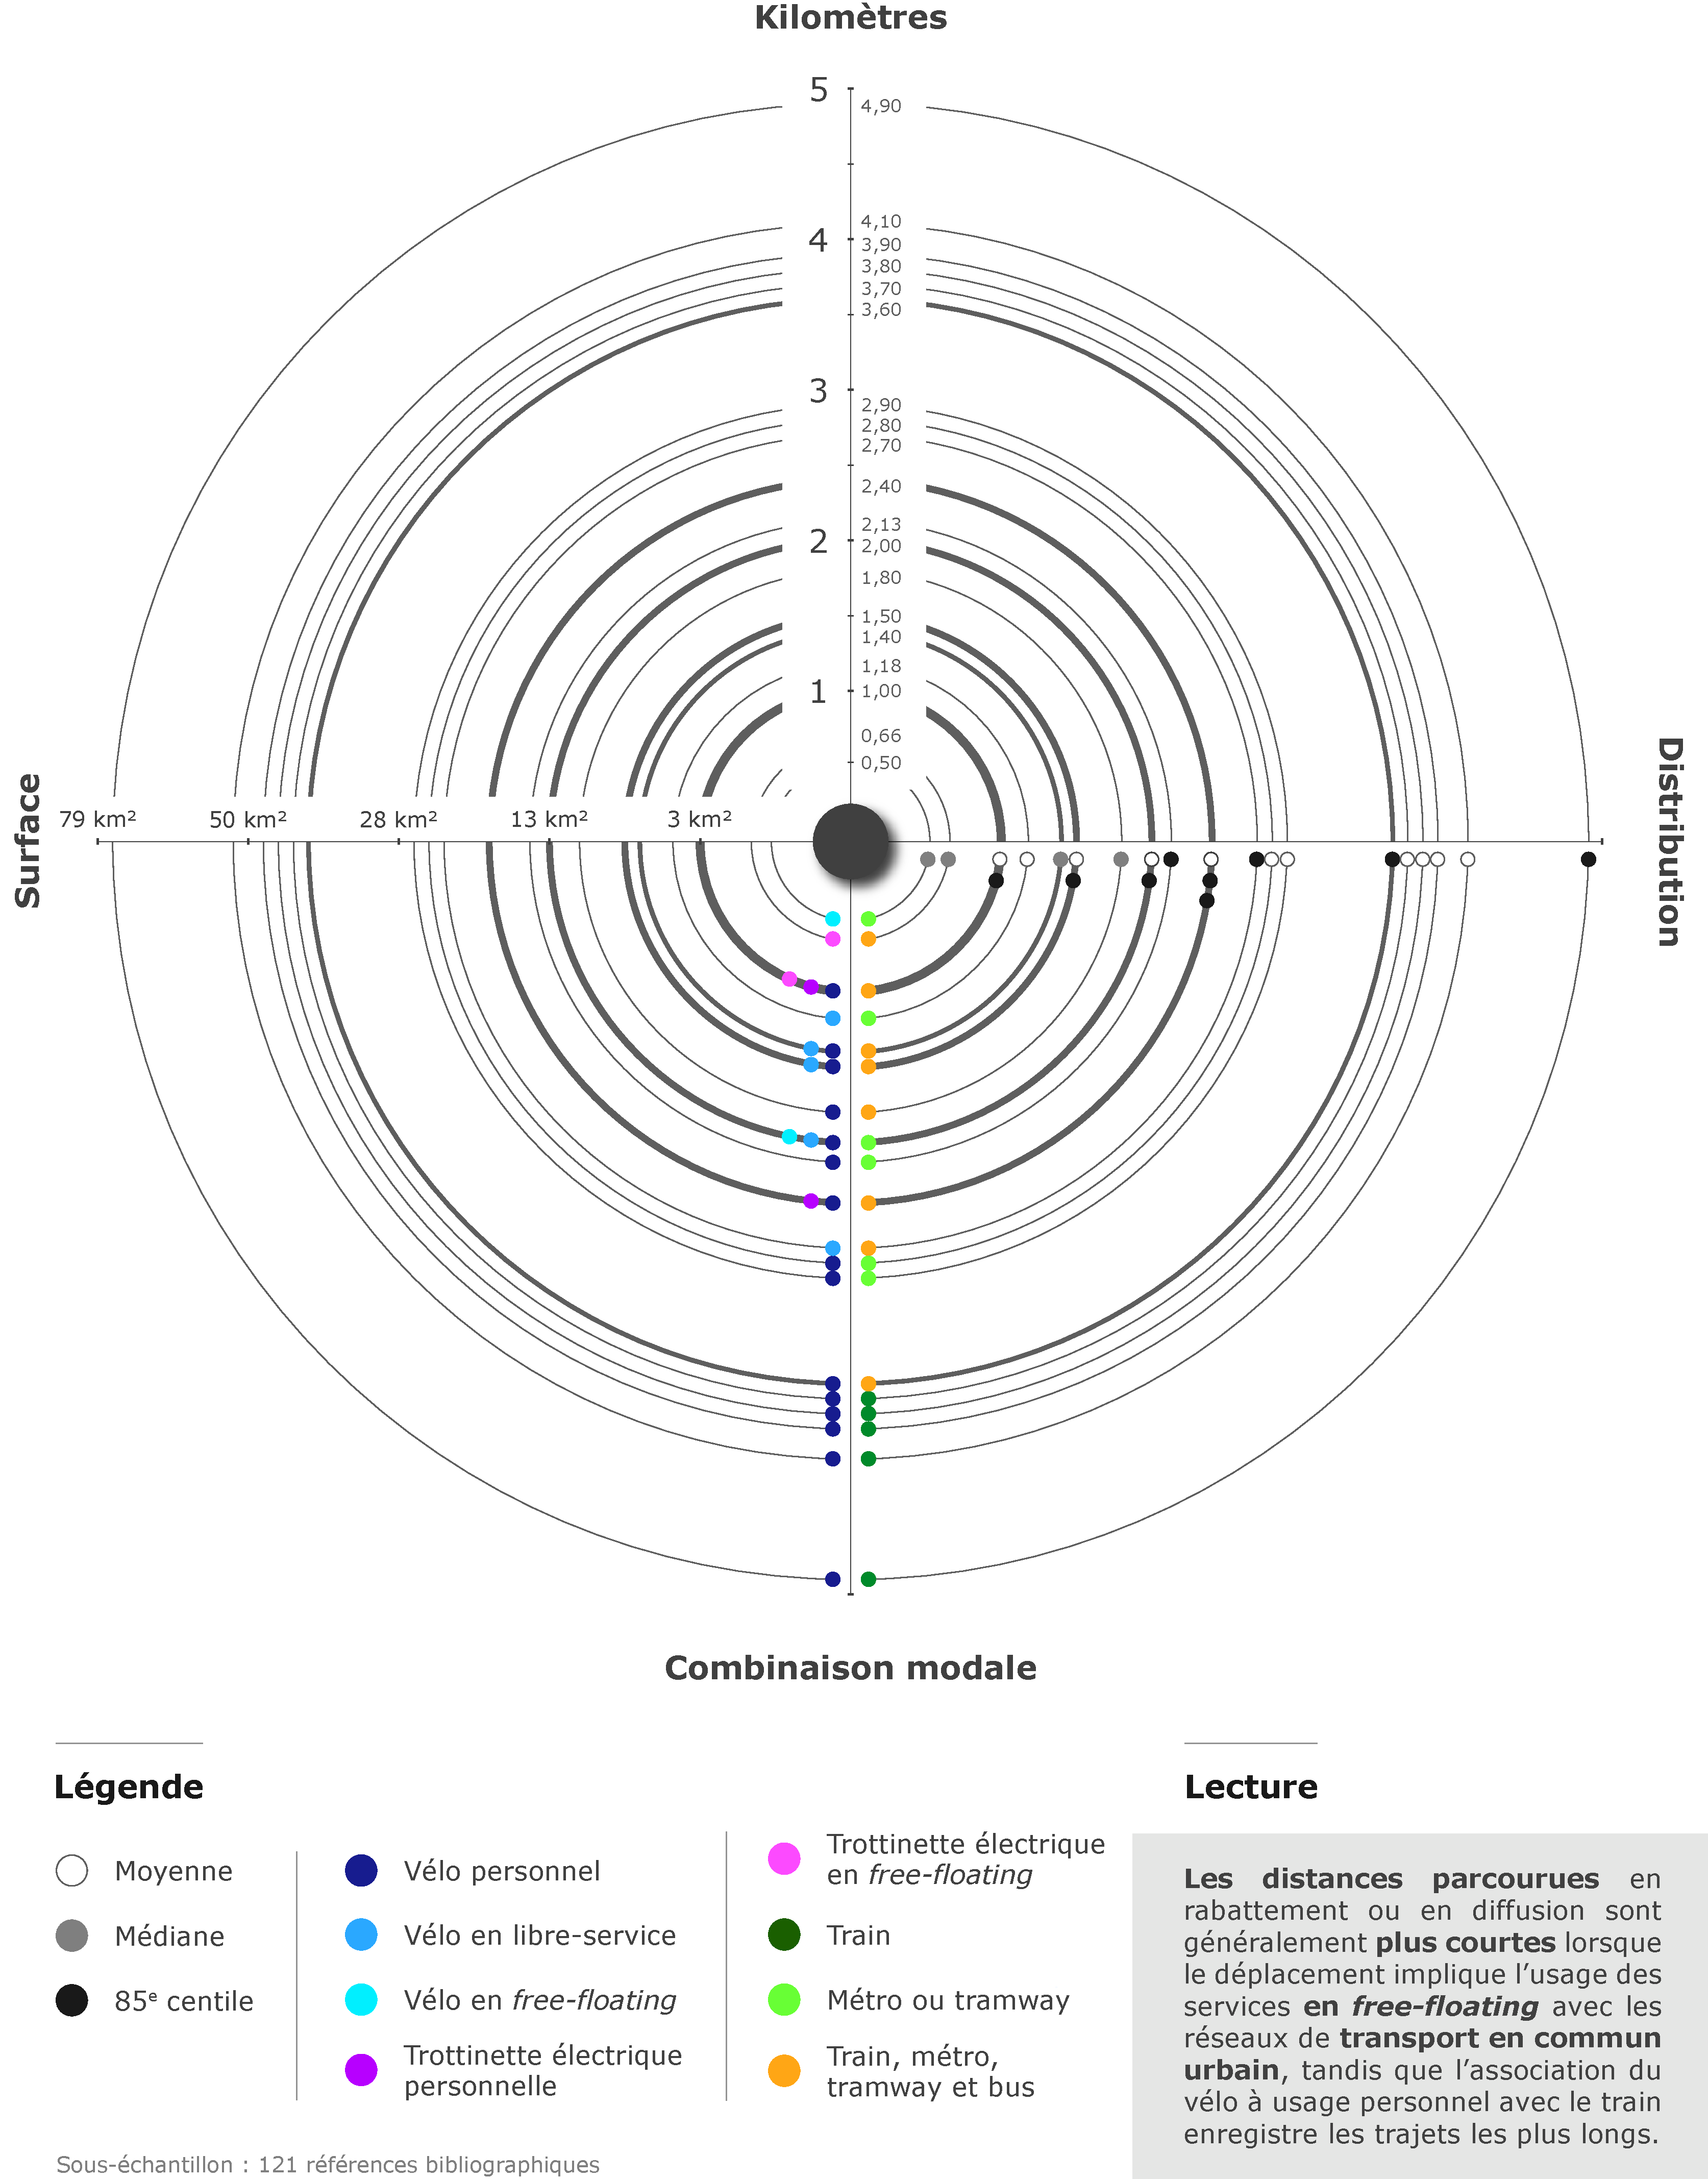
\includegraphics[width=1\columnwidth]{src/Figures/Chap-2/FR_RSL_Aires_influence.pdf}}
        \vspace{5pt}
        \begin{flushright}\scriptsize{
        Auteur~: \textcolor{blue}{Dylan Moinse (2023)}
        }\end{flushright}
    \end{figure}
    
    % Distances temps
La distance-temps en lien avec l'intermodalité est un aspect peu exploré dans la littérature scientifique, mais quelques études fournissent des aperçus importants sur la durée des déplacements combinant la mobilité individuelle légère et les transports en commun. À Shanghai, \textcolor{blue}{\textcite[19]{lin_analysis_2019}}\index{Lin, Diao|pagebf}\index{Zhang, Yongping|pagebf}\index{Zhu, Ruoxin|pagebf}\index{Meng, Liqiu|pagebf} évaluent la durée moyenne d'un trajet en \acrshort{VFF} pour accéder à une station de métro à 8,2~minutes, équivalant à deux kilomètres. À Utrecht, les déplacements en vélo personnel vers et depuis les stations de transport en commun révèlent des durées médianes distinctes~: en pré-acheminement vers les gares, la durée médiane est de 10,1~minutes, correspondant à une distance de 1,8 kilomètre, tandis qu'en post-acheminement depuis les gares, elle atteint 12,5 minutes, soit une distance de 2,4 kilomètres, selon \textcolor{blue}{\textcite[268]{krygsman_multimodal_2004}}\index{Krygsman, Stephan|pagebf}\index{Dijst, Martin|pagebf}\index{Arentze, Theo|pagebf}. Dans le contexte régional en Provence-Alpes-Côte d'Azur, \textcolor{blue}{\textcite[186]{moinse_intermodal_2022}}\index{Moinse, Dylan|pagebf}\index{Goudeau, Matthieu|pagebf}\index{L'Hostis, Alain|pagebf}\index{Leysens, Thomas|pagebf} constatent une durée moyenne de trajet en \acrshort{TEP} de 10,6 minutes en combinaison avec le train, équivalente à une distance de 2,4 kilomètres. L'utilisation du \acrshort{VLS} en association avec le métro et le bus présente un temps moyen de déplacement de 16 minutes, comme indiqué dans l'étude de cas sur Taipei \textcolor{blue}{\autocite[49]{lu_improving_2018}}\index{Lu, Miaojia|pagebf}\index{Hsu, Shu Chien|pagebf}\index{Chen, Pi Cheng|pagebf}\index{Lee, Wan Yu|pagebf}, tandis que cette combinaison atteint une valeur maximale (95\textsuperscript{e} centile) de 30~minutes à Nanjing \textcolor{blue}{\autocite[64]{ma_understanding_2018}}\index{Ma, Xinwei|pagebf}\index{Ji, Yanjie|pagebf}\index{Yang, Mingyuan|pagebf}\index{Jin, Yuchuan|pagebf}\index{Tan, Xu|pagebf}.%%Rédigé%%

    % 2.3.5.4. Aires d'influence
    \needspace{1\baselineskip} % Réserve de l'espace
\subsubsection*{Aires d'influence
    \label{chap2:aires-influence}
    }
    
    % <3km
La documentation analysée s'appuie sur un périmètre d'étude délimité et fondé sur la distribution des distances spatiales. Dans cette optique, plusieurs recherches académiques ont identifié des zones d'influence de portée relativement limitée, se concentrant essentiellement autour des arrêts de transport en commun urbain. Ainsi, \textcolor{blue}{\textcite[5]{wang_interchange_2016}}\index{Wang, Zi-jia|pagebf}\index{Chen, Feng|pagebf}\index{Xu, Tian-kun|pagebf} ont observé que les distances parcourues à vélo à Beijing se situent majoritairement entre~0,4~et~1,4~kilomètre. Selon les travaux de \textcolor{blue}{\textcite[11]{hu_examining_2022}}\index{Hu, Songhua|pagebf}\index{Chen, Mingyang|pagebf}\index{Jiang, Yuan|pagebf}\index{Sun, Wei|pagebf}\index{Xiong, Chenfeng|pagebf}, la distance spatiale pertinente en vue de modéliser l'utilisation du \acrshort{VFF} à Shanghai varie entre 1~et~1,5 kilomètre, les zones périurbaines étant caractérisées par des trajets généralement plus étendus. Ce même périmètre d'influence est également adopté par \textcolor{blue}{\textcite[9]{jin_competition_2019}}\index{Jin, Haitao|pagebf}\index{Jin, Fengjun|pagebf}\index{Wang, Jiao'e|pagebf}\index{Sun, Wei|pagebf}\index{Dong, Libo|pagebf} et par \textcolor{blue}{\textcite[10]{fan_how_2019}}\index{Fan, Aihua|pagebf}\index{Chen, Xumei|pagebf}\index{Wan, Tao|pagebf} dans le contexte urbain de Beijing, suggérant un rayon d'action établi jusqu'à deux kilomètres pour le \acrshort{VFF}. À Shanghai, \textcolor{blue}{\textcite[185]{pan_intermodal_2010}}\index{Pan, Haixiao|pagebf}\index{Shen, Qing|pagebf}\index{Xue, Song|pagebf} déterminent une aire s'étendant de 0,8~à~2,5 kilomètres, en soulignant que la majorité des déplacements à vélo et en \acrshort{VAE} se produisent sur des distances inférieures à 1,5 kilomètre. Selon \textcolor{blue}{\textcite[5]{ma_connecting_2022}}\index{Ma, Qingyu|pagebf}\index{Xin, Yanan|pagebf}\index{Yang, Hong|pagebf}\index{Xie, Kun|pagebf}, un périmètre compris entre deux et trois kilomètres a été établi pour apprécier la portée de la \acrshort{TEFF} à Washington~D.C., une démarche similaire étant observée à Beijing pour le \acrshort{VFF} \textcolor{blue}{\autocite[6]{ma_connecting_2022}}\index{Ma, Qingyu|pagebf}\index{Xin, Yanan|pagebf}\index{Yang, Hong|pagebf}\index{Xie, Kun|pagebf} ainsi qu'à Atlanta pour le vélo \textcolor{blue}{\autocite[57]{bearn_adaption_2018}}\index{Bearn, Cary|pagebf}\index{Mingus, Charlene|pagebf}\index{Watkins, Kari|pagebf}. Il convient de préciser que les seuils de distance mentionnés se rapportent spécifiquement aux réseaux de transport en commun urbain, comme le métro. Par conséquent, la configuration spatiale de ces infrastructures de transport, caractérisée par de courtes distances entre les stations, peut expliquer la taille réduite des zones d'influence mesurées.%%Rédigé%%

    % >3km
À partir d'un rayon de deux à trois kilomètres, les aires géographiques considérées s'avèrent être plus appropriées pour une utilisation intermodale du vélo en combinaison avec le train. Au travers d'une investigation sur les Pays-Bas, \textcolor{blue}{\textcite[227]{keijer_how_2000}}\index{Keijer, Majanka|pagebf}\index{Rietveld, Piet|pagebf} et \textcolor{blue}{\textcite[73]{rietveld_accessibility_2000}}\index{Rietveld, Piet|pagebf} introduisent un cadre de lecture prenant appui sur des facteurs de décroissance de la distance, justifiant ainsi l'établissement d'un périmètre étendu de 1~à~3,5 kilomètres, au-delà duquel l'attrait pour l'utilisation du vélo tend à diminuer. Cette observation est corroborée par les travaux de \textcolor{blue}{\textcite[281]{debrezion_modelling_2009}}\index{Debrezion, Ghebreegziabiher|pagebf}\index{Pels, Eric|pagebf}\index{Rietveld, Piet|pagebf}, qui confirment que le vélo est compétitif pour des distances allant de 1,1~à~4,2~kilomètres vers ou depuis la gare. Diverses productions scientifiques étendent l'aire d'influence jusqu'à cinq kilomètres, comme en témoignent l'utilisation du \acrshort{VFF} à Shenzhen \textcolor{blue}{\autocite[6]{wu_measuring_2019}}\index{Wu, Xueying|pagebf}\index{Lu, Li|pagebf}\index{Lin, Yaoyu|pagebf}\index{Yang, Yiyang|pagebf}, ou encore l'association du \acrshort{VLS} et du vélo avec le métro à Beijing \textcolor{blue}{\autocite[54]{zhao_bicycle-metro_2017}}\index{Zhao, Pengjun|pagebf}\index{Li, Shengxiao|pagebf}. La même zone d'impact est identifiée concernant la combinaison entre le vélo et le train, que ce soit à Amboise \textcolor{blue}{\autocite[751]{midenet_modal_2018}}\index{Midenet, Sophie|pagebf}\index{Côme, Etienne|pagebf}\index{Papon, Francis|pagebf}, à Göteborg, Malmö et Beijing \textcolor{blue}{\autocite[15]{hamidi_shaping_2020}}\index{Hamidi, Zahra|pagebf}\index{Zhao, Chunli|pagebf}, à El Monte \textcolor{blue}{\autocite[118]{cottrell_transforming_2007}}\index{Cottrell, Wayne~D.|pagebf} ou encore à Xi'an \textcolor{blue}{\autocite[172]{yang_bike-and-ride_2014}}\index{Yang, Liu|pagebf}\index{Chao, Li|pagebf}\index{Wang, Yuanqing|pagebf}. Allant encore plus loin, \textcolor{blue}{\textcite[9]{kim_analysis_2021}}\index{Kim, Minjun|pagebf}\index{Cho, Gi-Hyoung|pagebf} soutiennent que les déplacements combinant le \acrshort{VLS} et le métro à Séoul sont fréquents jusqu'à une distance de dix kilomètres, soulignant ainsi la portée étendue de ces pratiques intermodales.%%Rédigé%%

    % Temps
Dans une perspective temporelle, une partie de la documentation académique s'est attachée à déterminer les zones d'influence des stations de transport en commun, en prenant en compte la variable temporelle. À cet égard, \textcolor{blue}{\textcite[18, 21]{li_factors_2020}}\index{Li, Xuefeng|pagebf}\index{Du, Mingyang|pagebf}\index{Yang, Jingzong|pagebf} ont mis en évidence que les déplacements en \acrshort{VFF} d'une durée inférieure à sept minutes prédominent, spécialement durant les périodes de pointe matinales en semaine, bien que certaines régions de Shenzhen, y compris son centre urbain, affichent une majorité de trajets excédant quinze minutes. Selon \textcolor{blue}{\textcite[128]{liu_understanding_2020}}\index{Liu, Yang|pagebf}\index{Ji, Yanjie|pagebf}\index{Feng, Tao|pagebf}\index{Timmermans, Harry~J.~P.|pagebf}, un temps de parcours à vélo supérieur à dix minutes réduit son usage en combinaison avec le métro à Nanjing. Cette durée s'établit à douze minutes pour l'usage conjoint du \acrshort{VLS} et du réseau ferroviaire à Boston, Chicago, Washington~D.C., et à New York City \textcolor{blue}{\autocite[9]{kong_deciphering_2020}}\index{Kong, Hui|pagebf}\index{Jin, Scarlett~T.|pagebf}\index{Sui, Daniel~Z.|pagebf}, et s'étend à quinze minutes pour le \acrshort{VLS} en association avec le train à Osaka \textcolor{blue}{\autocite[3415]{tomita_demand_2017}}\index{Tomita, Yasuo|pagebf}\index{Nakayama, Akihiko|pagebf}. \textcolor{blue}{\textcite[5]{yang_empirical_2016}}\index{Yang, Min|pagebf}\index{Liu, Xinlu|pagebf}\index{Wang, Wei|pagebf}\index{Li, Zhibin|pagebf}\index{Zhao, Jingyao|pagebf} délimitent, quant à eux, un périmètre temporel de vingt minutes pour l'usage du \acrshort{VLS} en relation avec le réseau de métro à Nanjing. Enfin, \textcolor{blue}{\textcite[1696]{cheng_evaluating_2012}}\index{Cheng, Yung-Hsiang|pagebf}\index{Liu, Kuo-Chu|pagebf} adoptent une approche plus systémique en mesurant simultanément les temps de trajet en rabattement et en diffusion, observant ainsi que la majorité des cyclistes utilisant le métro à Kaohsiung effectuent des parcours de moins de trente minutes aller et retour.%%Rédigé%%

    % 2.3.5.5. Variabilité des distances et détours
    \needspace{1\baselineskip} % Réserve de l'espace
\subsubsection*{Variabilité des distances
    \label{chap2:variabilite-distances}
    }

    % Facteurs
L'évaluation des distances effectivement parcourues par les voyageur·se·s intermodaux·les, en particulier pour les \Guillemets{premiers et derniers kilomètres}, dépend étroitement des choix d'itinéraires adoptés. Ces trajets, empruntés par les cyclistes, sont influencés par une diversité de facteurs relatifs à l'environnement urbain, au contexte temporel ainsi qu'aux comportements, aux habitudes et aux expériences de mobilité. Selon \textcolor{blue}{\textcite[15]{tzouras_describing_2023}}\index{Tzouras, Panagiotis|pagebf}\index{Mitropoulos, Lambros|pagebf}\index{Koliou, Katerina|pagebf}\index{Stavropoulou, Eirini|pagebf}\index{Karolemeas, Christos|pagebf}\index{Antoniou, Eleni|pagebf}\index{Karaloulis, Antonis|pagebf}\index{Mitropoulos, Konstantinos|pagebf}\index{Vlahogianni, Eleni~I.|pagebf}\index{Kepaptsoglou, Konstantinos|pagebf}, les utilisateur·rice·s de la \acrshort{TEP} à Athènes sélectionnent leurs parcours en tenant compte de la sécurité perçue et de la distance minimale, dans le but d'atteindre un équilibre entre l'effort physique requis et les obstacles tant physiques que psychologiques à éviter. \textcolor{blue}{\textcite[621]{krizek_detailed_2007}}\index{Krizek, Kevin~J.|pagebf}\index{El-Geneidy, Ahmed~M.|pagebf}\index{Thompson, Kristin|pagebf} observent que les distances mesurées sont également déterminées par le motif de déplacement~: les trajets à vélo et en tramway associés aux achats et au travail sont plus courts, tandis que ceux liés aux loisirs sont plus longs, à Minneapolis. Le contexte environnemental et temporel a aussi un impact notable sur les distances parcourues. À cet égard, \textcolor{blue}{\textcite[619]{krizek_detailed_2007}}\index{Krizek, Kevin~J.|pagebf}\index{El-Geneidy, Ahmed~M.|pagebf}\index{Thompson, Kristin|pagebf} démontrent que les cyclistes préfèrent rallonger leur trajet jusqu'à 67~\% pour atteindre un itinéraire cyclable de bonne qualité. \textcolor{blue}{\textcite[8]{adnan_last-mile_2019}}\index{Adnan, Muhammad|pagebf}\index{Altaf, Shahbaz|pagebf}\index{Bellemans, Tom|pagebf}\index{Yasar, Ansar-ul-Haque|pagebf}\index{Shakshuki, Elhadi~M.|pagebf} ont démontré que les usager·ère·s du \acrshort{VLS} dans des villes de taille moyenne en Belgique sont sensibles à des facteurs météorologiques tels que la température et la pluviométrie, influençant non seulement les itinéraires, mais également le choix modal. Les utilisateur·rice·s du \acrshort{VLS} à Séoul sont plus sensibles à la distance en soirée, par rapport aux autres moments de la journée, selon \textcolor{blue}{\autocite[3110]{cho_estimation_2022}}\index{Cho, Shin-Hyung|pagebf}\index{Shin, DongHwa|pagebf}. À Nanjing, \textcolor{blue}{\textcite[11]{li_operating_2019}}\index{Li, Yuan|pagebf}\index{Zhu, Zhenjun|pagebf}\index{Guo, Xiucheng|pagebf} ont révélé que la portée du \acrshort{VFF} varie en fonction du jour de la semaine et du type de station de métro. Ces enseignements sont en accord avec les conclusions de \textcolor{blue}{\textcite[105]{flamm_public_2014}}\index{Flamm, Bradley~J.|pagebf}\index{Rivasplata, Charles~R.|pagebf}, qui ont remarqué que les distances parcourues par les cyclistes à Philadelphie et à San Francisco dépendent du type de transport en commun et de la topographie. De plus, le train enregistre des distances plus longues comparativement aux services conventionnels et \textsl{express} de bus, représentant une variable plus significative que les facteurs socio-démographiques, lesquels ont un impact modéré sur la distance dans plusieurs métropoles étasuniennes \textcolor{blue}{\autocite[23-24]{hochmair_assessment_2015}}\index{Hochmair, Hartwig~H.|pagebf}. Finalement, les stations de métro situées en périphérie de Shanghai présentent des aires d'attraction nettement plus vastes que celles du centre urbain \textcolor{blue}{\autocite[8]{yu_policy_2021}}\index{Yu, Qing|pagebf}\index{Li, Weifeng|pagebf}\index{Yang, Dongyuan|pagebf}\index{Xie, Yingkun|pagebf}. Cette pluralité de facteurs affectant le rapport à la distance illustre à quel point les cyclistes ne privilégient pas systématiquement l'itinéraire le plus court, révélant ainsi des stratégies visant à équilibrer optimisation spatio-temporelle et confort.%%Rédigé%%

    % Détours
Plusieurs travaux de recherche mettent en exergue la pratique de détours par les voyageur·se·s intermodaux·les, qui parcourent des distances accrues en raison de multiples facteurs. Selon \textcolor{blue}{\textcite[102]{kampen_understanding_2020}}\index{Kampen, Jullian van|pagebf}\index{Jayaraj, Manoj Ashvin|pagebf}\index{Pauwels, Eric|pagebf}\index{Mei, Rob van der|pagebf}\index{Dugundji, Elenna~R.|pagebf}, 42~\% des cyclistes sont enclin·e·s à se diriger vers des gares plus éloignées que la gare la plus proche, privilégiant celles dotées d'une meilleure connectivité, dans les régions de North-Holland, South-Holland, Flevoland et d'Utrecht. D'une part, \textcolor{blue}{\textcite[18]{jonkeren_bicycle-train_2021}}\index{Jonkeren, Olaf|pagebf}\index{Kager, Roland|pagebf}\index{Harms, Lucas|pagebf}\index{te Brömmelstroet, Marco|pagebf} soulignent l'objectif de contourner les ruptures de charge en favorisant des gares mieux équipées, comme celles d'Utrecht, Rotterdam et d'Eindhoven. D'autre part, cette préférence s'étend également aux stations de métro offrant des infrastructures de stationnement pour vélos, comme le montre l'étude de cas à Amsterdam conduite par \textcolor{blue}{\textcite[342]{kampen_bicycle_2021}}\index{Kampen, Jullian van|pagebf}\index{Pauwels, Eric|pagebf}\index{Mei, Rob van der|pagebf}\index{Dugundji, Elenna~R.|pagebf}. À Shanghai, \textcolor{blue}{\textcite[7]{li_exploring_2021}}\index{Li, Wenxiang|pagebf}\index{Chen, Shawen|pagebf}\index{Dong, Jieshuang|pagebf}\index{Wu, Jingxian|pagebf} révèlent que les stations de transport en commun les plus fréquentées attirent des passager·ère·s en \acrshort{VFF} de plus loin. \textcolor{blue}{\textcite[143]{kampen_understanding_2021}}\index{Kampen, Jullian van|pagebf}\index{Jayaraj, Manoj Ashvin|pagebf}\index{Pauwels, Eric|pagebf}\index{Mei, Rob van der|pagebf}\index{Dugundji, Elenna~R.|pagebf} ajoutent que les cyclistes avec un revenu net mensuel inférieur à 2~500€ et âgé·e·s de plus de 39 ans sont davantage susceptibles de se rendre à la seconde gare la plus proche de leur lieu de départ. Le rôle de facteurs venant influencer les distances effectives parcourues reflète l'importance des politiques et des stratégies visant à orienter la mobilité des personnes, de sorte à rendre les systèmes de mobilité alternatifs plus attrayants face à l'utilisation de l'automobile.%%Rédigé%%

    % 2.3.6. Resultats : management de la demande
    \needspace{1\baselineskip} % Réserve de l'espace
\subsection{Gestion de la demande de mobilité
    \label{chap2:gestion-demande-mobilite}
    }

    % Introduction
La gestion de la demande en mobilité, englobant l'ensemble des stratégies et politiques visant à orienter les choix de déplacement des individus, est au cœur de 61~études scientifiques traitant du \acrshort{M-TOD}. Notre analyse débutera par l'examen du rôle du niveau de services offert par les systèmes de transport en commun et l'importance de la mise en place d'une tarification intégrée. Nous aborderons ensuite la contribution des services de mobilité partagée, ainsi que le rôle des réseaux de bus dans les quartiers de gare. Enfin, cette section traitera de la gestion de la circulation et du stationnement automobile.%%Rédigé%%

    % 2.3.6.1. Fréquence et temps d'attente
    \needspace{1\baselineskip} % Réserve de l'espace
\subsubsection*{Niveau de service du \textsl{mass transit}
    \label{chap2:niveau-service}
    }
    
    % Fréquence des TC
Une desserte ferroviaire régulière et ponctuelle semble favoriser la pratique intermodale impliquant l'usage du vélo. Cette observation a été relevée pour les trains dans la Randstad South \textcolor{blue}{\autocite[45]{la_paix_puello_modelling_2015}}\index{La Paix Puello, Lissy|pagebf}\index{Geurs, Karst~T.|pagebf}, à Rotterdam \textcolor{blue}{\autocite[5]{montes_shared_2023}}\index{Montes, Alejandro|pagebf}\index{Geržinic, Nejc|pagebf}\index{Veeneman, Wijnand|pagebf}\index{Oort, Niels van|pagebf}\index{Hoogendoorn, Serge|pagebf}, à Turin \textcolor{blue}{\autocite[12]{staricco_implementing_2020}}\index{Staricco, Luca|pagebf}\index{Vitale Brovarone, Elisabetta|pagebf}, et à Shanghai pour le \acrshort{VFF} en association avec le métro \textcolor{blue}{\autocite[24]{lin_analysis_2019}}\index{Lin, Diao|pagebf}\index{Zhang, Yongping|pagebf}\index{Zhu, Ruoxin|pagebf}\index{Meng, Liqiu|pagebf}. À Melbourne, \textcolor{blue}{\textcite[401]{weliwitiya_bicycle_2019}}\index{Weliwitiya, Hesara|pagebf}\index{Rose, Geoff|pagebf}\index{Johnson, Marilyn|pagebf} ont mis en évidence une corrélation positive entre la fréquence des lignes ferroviaires, en particulier pendant les heures de pointe matinales, et le taux d'utilisation du vélo comme mode de rabattement. Les auteur·rice·s constatent qu'une augmentation d'une unité de fréquence entraîne une augmentation de 1,03 du nombre de cyclistes intermodaux·les. À Poznań, \textcolor{blue}{\textcite[199]{radzimski_exploring_2021}}\index{Radzimski, Adam|pagebf}\index{Dzięcielski, Michał|pagebf} ont mis en évidence une corrélation positive entre la fréquence des lignes de tramway et le nombre de trajets en \acrshort{VLS} pour des distances courtes, jusqu'à 1,5 kilomètre, ainsi que pour des distances moyennes, entre 1,5 et 3 kilomètres, mais cette relation n'est pas observée pour les trajets excédant 3 kilomètres. Cependant, \textcolor{blue}{\textcite[301]{kuijk_preferences_2022}}\index{Mil, Joeri~F.P. van|pagebf}\index{Leferink, Tessa~S.|pagebf}\index{Annema, Jan Anne|pagebf}\index{Oort, Niels van|pagebf}\index{Kuijk, Roy~J. van|pagebf}\index{Almeida Correia, Gonçalo Homem de|pagebf}\index{Oort, Niels van|pagebf}\index{Arem, Bart van|pagebf} n'ont identifié aucun paramètre significatif concernant la fréquence et la vitesse du tramway en lien avec l'utilisation du \acrshort{VLS} à Utrecht. Par ailleurs, les résultats des études réalisées par \textcolor{blue}{\textcite[41]{nielsen_bikeability_2018}}\index{Nielsen, Thomas Alexander Sick|pagebf}\index{Skov-Petersen, Hans|pagebf} suggèrent que la fréquence des services ferroviaires pourrait diminuer la probabilité de recourir au vélo au Danemark.%%Rédigé%%

    % Densité des stations
Au-delà de la fréquence des services de transport public, la vitesse commerciale de ces modes collectifs, intrinsèquement liée au temps de voyage, s'avère être un facteur déterminant dans le choix modal en faveur du vélo. Cette tendance contraste avec le rôle mineur attribué à la ponctualité et à la sécurité des services ferroviaires à Eindhoven \textcolor{blue}{\autocite[727]{waerden_relation_2018}}\index{Waerden, Peter|pagebf}\index{Waerden, Jaap|pagebf}. La vitesse du trajet en transport public est largement influencée par la densité des stations, qui a un impact significatif sur la demande de transfert à vélo. En effet, des gares très rapprochées tendent à réduire la probabilité d'opter pour ce mode de déplacement au Danemark \textcolor{blue}{\autocite[41]{nielsen_bikeability_2018}}\index{Nielsen, Thomas Alexander Sick|pagebf}\index{Skov-Petersen, Hans|pagebf}. Au contraire, la densité des stations de métro affecte positivement l'utilisation du \acrshort{VLS} à Nanjing \textcolor{blue}{\autocite[17]{ji_exploring_2018}}\index{Ji, Yanjie|pagebf}\index{Ma, Xinwei|pagebf}\index{Yang, Mingyuan|pagebf}\index{Jin, Yuchuan|pagebf}\index{Gao, Liangpeng|pagebf}. En explorant la combinaison du \acrshort{VFF} et du métro à Beijing, \textcolor{blue}{\textcite[10]{guo_exploring_2023}}\index{Guo, Dongbo|pagebf}\index{Yao, Enjian|pagebf}\index{Liu, Shasha|pagebf}\index{Chen, Rongsheng|pagebf}\index{Hong, Junyi|pagebf}\index{Zhang, Junyi|pagebf} ont constaté que le temps d'attente a pour autant un impact bien plus négatif que le temps de trajet lui-même~–~les usager·ère·s étant prêt·e·s à payer 13,6~\euro~ (105 CNY) pour économiser une heure d'attente, contre 2~\euro~ (15 CNY) pour une heure de \acrshort{VFF}~–, soulignant ainsi la nécessité d'établir des connexions efficaces au sein du système de transport public pour répondre à l'aversion face au temps de transfert.%%Rédigé%%

    % 2.3.6.2. MaaS et tarification
    \needspace{1\baselineskip} % Réserve de l'espace
\subsubsection*{Tarification intégrée
    \label{chap2:tarification_integree}
    }
    
    % MaaS
Pour favoriser l'intégration et encourager ces pratiques intermodales, la littérature scientifique préconise de simplifier les connexions entre différents systèmes de mobilité en promouvant l'utilisation de cartes de transport intégrées \textcolor{blue}{\autocite[172]{yang_bike-and-ride_2014}}\index{Yang, Liu|pagebf}\index{Chao, Li|pagebf}\index{Wang, Yuanqing|pagebf}, la mesure la plus plébiscitée par les passager·ère·s \textcolor{blue}{\autocite[10]{yang_empirical_2016}}\index{Yang, Min|pagebf}\index{Liu, Xinlu|pagebf}\index{Wang, Wei|pagebf}\index{Li, Zhibin|pagebf}\index{Zhao, Jingyao|pagebf}. L'un des principaux leviers d'action identifiés concerne la mobilité individuelle légère partagée et la mise en œuvre d'une plateforme multimodale de type \acrshort{MaaS}, offrant notamment la possibilité de mutualiser, voire d'unifier le paiement en ligne \textcolor{blue}{\autocite[5]{fearnley_patterns_2020}}\index{Fearnley, Nils|pagebf}\index{Johnsson, Espen|pagebf}\index{Berge, Siri Hegna|pagebf}. À Nanjing, un manque d'information sur les installations de location de vélos a été constaté, malgré un intérêt manifeste pour ce service, soulignant l'importance du \acrshort{MaaS} \textcolor{blue}{\autocite[136]{chen_determinants_2012}}\index{Chen, Lijun|pagebf}\index{Pel, Adam~J.|pagebf}\index{Chen, Xuewu|pagebf}\index{Sparing, Daniel|pagebf}\index{Hansen, Ingo~A.|pagebf}. Selon \textcolor{blue}{\textcite[67]{ma_understanding_2018}}\index{Ma, Xinwei|pagebf}\index{Ji, Yanjie|pagebf}\index{Yang, Mingyuan|pagebf}\index{Jin, Yuchuan|pagebf}\index{Tan, Xu|pagebf}, les plateformes intégrées devraient inclure un programme de fidélité pour privilégier les utilisateur·rice·s fréquent·e·s du \acrshort{VLS} et des transports en commun, en réservant certains emplacements de vélopartage à ces usager·ère·s. Cependant, \textcolor{blue}{\textcite[12]{fan_how_2019}}\index{Fan, Aihua|pagebf}\index{Chen, Xumei|pagebf}\index{Wan, Tao|pagebf} soulignent des obstacles liés à l'utilisation du \acrshort{VFF} ou d'une plate-forme \acrshort{MaaS} à Beijing, tels que la nécessité d'installer une application mobile, de fournir des informations personnelles pour s'enregistrer et de verser un dépôt de garantie important, alors que la tarification reste le principal facteur influençant le choix du \acrshort{VFF}.%%Rédigé%%

    % Tarification vélopartage et micro-mobilité partagée
Les coûts du vélo et de la micro-mobilité en libre-service sont souvent jugés prohibitifs et ne favorisent pas leur utilisation en rabattement et d'autant plus en diffusion \textcolor{blue}{\autocite[5]{montes_shared_2023}}\index{Montes, Alejandro|pagebf}\index{Geržinic, Nejc|pagebf}\index{Veeneman, Wijnand|pagebf}\index{Oort, Niels van|pagebf}\index{Hoogendoorn, Serge|pagebf}. À Nanjing, les jeunes travailleurs choisissent le \acrshort{VLS} pour des raisons économiques, ce qui soulève des interrogations sur les stratégies tarifaires ne favorisant pas le maintien de ces pratiques de mobilité vertueuses à long terme. À cet égard, les coûts d'un trajet unique et d'un abonnement au service ont un impact considérable sur le choix du \acrshort{VFF} pour accéder au réseau de métro \textcolor{blue}{\autocite[17]{zhong_layout_2021}}\index{Zhong, Hongming|pagebf}\index{Liu, Zijian|pagebf}\index{Chen, Jun|pagebf}\index{Hao, Jun|pagebf}\index{Wang, Wei|pagebf}. À Beijing, les voyageur·se·s ayant recours au \acrshort{VFF} dépensent presque autant pour des trajets courts à l'aide de ce service que pour le trajet en transport en commun \textcolor{blue}{\autocite[12]{fan_how_2019}}\index{Fan, Aihua|pagebf}\index{Chen, Xumei|pagebf}\index{Wan, Tao|pagebf}. Plusieurs solutions émergent de ces constats. À Nanjing, un temps gratuit de location de vélo de deux heures, comme politique de promotion efficace pour 57~\% des voyageur·se·s, a été identifié par \textcolor{blue}{\textcite[135]{chen_determinants_2012}}\index{Chen, Lijun|pagebf}\index{Pel, Adam~J.|pagebf}\index{Chen, Xuewu|pagebf}\index{Sparing, Daniel|pagebf}\index{Hansen, Ingo~A.|pagebf}. À Washington~D.C. et Los Angeles, des incitations tarifaires favorisant l'utilisation de la \acrshort{TEFF} avec le métro sont évaluées, notamment avec des réductions de prix lorsqu'un crédit de 2,8~\euro~ (3~\$) est appliqué sur les tarifs de la trottinette \textcolor{blue}{\autocite[11]{yan_evaluating_2023}}\index{Yan, Xiang|pagebf}\index{Zhao, Xilei|pagebf}\index{Broaddus, Andrea|pagebf}\index{Johnson, Joshua|pagebf}\index{Srinivasan, Sivaramakrishnan|pagebf}. À Boston et Worcester, l'impact de différents schémas tarifaires est analysé, révélant que la combinaison d'un tarif fixe et basé sur la distance a le moins d'impact sur la demande de vélo associé au train \textcolor{blue}{\autocite[16]{fournier_continuous_2021}}\index{Fournier, Nicholas|pagebf}\index{Christofa, Eleni|pagebf}\index{Gonzales, Eric~J.|pagebf}, tandis qu'à Oslo, le prix à la minute est un facteur important pour promouvoir l'usage de la \acrshort{TEFF} avec les transports en commun \textcolor{blue}{\autocite[5]{fearnley_patterns_2020}}\index{Fearnley, Nils|pagebf}\index{Johnsson, Espen|pagebf}\index{Berge, Siri Hegna|pagebf}. Une tarification sociale basée sur les revenus est jugée efficace pour le \acrshort{VFF} et la \acrshort{TEFF} à Seattle afin d'atténuer les barrières financières \textcolor{blue}{\autocite[975-977]{beale_integrating_2023}}\index{Beale, Kirsten|pagebf}\index{Kapatsila, Bogdan|pagebf}\index{Grisé, Emily|pagebf}.%%Rédigé%%

    % Tarification usage TC et stationnement vélo
Enfin, le coût monétaire affecte aussi l'utilisation des transports en commun ainsi que le stationnement du vélo et de la micro-mobilité à usage personnel. La gratuité des services ferroviaires ciblée pour les étudiants aux Pays-Bas attire plus de cyclistes intermodaux·les aux dépens de l'automobile \textcolor{blue}{\autocite[360]{givoni_access_2007}}\index{Givoni, Moshe|pagebf}\index{Rietveld, Piet|pagebf}. Une aversion significative au coût de stationnement des vélos est observée chez les étudiant·e·s néerlandais·e·s \textcolor{blue}{\autocite[667]{mil_insights_2020}}\index{Mil, Joeri~F.P. van|pagebf}\index{Leferink, Tessa~S.|pagebf}\index{Annema, Jan Anne|pagebf}\index{Oort, Niels van|pagebf}. Cependant, \textcolor{blue}{\textcite[10]{molin_bicycle_2015}}\index{Molin, Eric|pagebf}\index{Maat, Kees|pagebf} indiquent que la gratuité du stationnement vélo n'influence pas l'usage du vélo en intermodalité aux Pays-Bas et qu'au contraire, 65~\% des cyclistes interrogé·e·s privilégient le scénario basé sur un stationnement sécurisé, mais payant avec un prix optimal à hauteur d'1,50~\euro~. De même, \textcolor{blue}{\textcite[5]{liu_mode_2022}}\index{Liu, Lumei|pagebf}\index{Kong, Hui|pagebf}\index{Liu, Tianliang|pagebf}\index{Ma, Xiaolei|pagebf} constatent que le coût du trajet a peu d'impact sur le choix entre le bus ou le \acrshort{VFF} en modes de transfert avec le métro à Beijing, suggérant que la qualité de l'infrastructure de vélopartage est un aspect plus important à prendre en compte.%%Rédigé%%

    % 2.3.6.3. Vélopartage et micro-mobilité partagée
    \needspace{1\baselineskip} % Réserve de l'espace
\subsubsection*{Services de transfert
    \label{chap2:services-transfert}
    }
    
    % Présence de vélopartage
La mise à disposition de systèmes de mobilité partagée, tels que le \acrshort{VLS}, le \acrshort{VFF} ou la \acrshort{TEFF}, s'avère être un élément fondamental pour l'intégration du vélo avec les transports en commun \textcolor{blue}{\autocite[11-12]{wu_measuring_2019}}\index{Wu, Xueying|pagebf}\index{Lu, Li|pagebf}\index{Lin, Yaoyu|pagebf}\index{Yang, Yiyang|pagebf}. Dès lors, l'incorporation de ces services de mobilité au sein de la stratégie urbaine du \acrshort{TOD} est préconisée afin d'accroître l'utilisation et l'efficacité globale du système de mobilité \textcolor{blue}{\autocite[16]{tamakloe_determinants_2021}}\index{Tamakloe, Reuben|pagebf}\index{Hong, Jungyeol|pagebf}\index{Tak, Jihoon|pagebf}. La disponibilité de vélos et d'options de micro-mobilité en libre-service à proximité des nœuds de transport en commun augmente non seulement la probabilité de leur utilisation comme modes de liaison \textcolor{blue}{\autocite[25]{guo_dockless_2021}}\index{Guo, Yuanyuan|pagebf}\index{Yang, Linchuan|pagebf}\index{Lu, Yi|pagebf}\index{Zhao, Rui|pagebf}, mais ces systèmes contribuent également à promouvoir une pratique plus efficace de l'intermodalité-voyageur·se·s, en réduisant la nécessité d'un second vélo \textcolor{blue}{\autocite[10]{jonkeren_bicycle_2021}}\index{Jonkeren, Olaf|pagebf}\index{Kager, Roland|pagebf}. À Shanghai, \textcolor{blue}{\textcite[186]{pan_intermodal_2010}}\index{Pan, Haixiao|pagebf}\index{Shen, Qing|pagebf}\index{Xue, Song|pagebf} ont identifié une forte volonté exprimée par les participant·e·s de l'étude d'utiliser des systèmes de location de vélos près des stations de métro. Partant du constat que les voyageur·se·s intermodaux·les disposent d'un haut degré de planification de leurs déplacements et adaptent leur comportement en fonction de l'offre de mobilité et des contraintes liées au transport et au stationnement du vélo, \textcolor{blue}{\textcite[196]{sherwin_practices_2011}}\index{Sherwin, Henrietta|pagebf}\index{Parkhurst, Graham|pagebf}\index{Robbins, Derek|pagebf}\index{Walker, Ian|pagebf} justifient la mise en place d'un système de location de vélos organisé à l'échelle nationale, à l'image de ce qui est pratiqué par les gestionnaires ferroviaires néerlandais et allemands.%%Rédigé%%

    % Gestion et réallocation des services de vélopartage et micro-mobilité partagée
La mise en place d'un système de mobilité individuelle légère partagée requiert une gestion efficace et une répartition optimale des flottes. Les travaux de \textcolor{blue}{\textcite[197]{radzimski_exploring_2021}}\index{Radzimski, Adam|pagebf}\index{Dzięcielski, Michał|pagebf} démontrent que la structuration d'un système de \acrshort{VLS}, organisé sous la forme de vélos en libre-service avec des stations dédiées, attire davantage d'usager·ère·s en combinaison avec le tramway par rapport au \acrshort{VFF}. De ce fait, il est recommandé d'améliorer l'allocation des \acrshort{VFF} en redistribuant de manière plus efficiente les vélos vers des espaces verts, des zones commerciales et industrielles, ainsi que des quartiers résidentiels à Beijing \textcolor{blue}{\autocite[12]{liu_temporal_2022}}\index{Liu, Siyang|pagebf}\index{Zhang, Xiaodong|pagebf}\index{Zhou, Chenjing|pagebf}\index{Rong, Jian|pagebf}\index{Bian, Yang|pagebf}. Face aux limitations de capacité des systèmes en \textsl{free-floating} lors de pics d'utilisation, comme cela a été observé pour la \acrshort{TEFF} à Columbus \textcolor{blue}{\autocite[9]{liu_measuring_2022}}\index{Liu, Luyu|pagebf}\index{Miller, Harvey~J.|pagebf}, \textcolor{blue}{\textcite[69, 95]{nat_bicycle_2018}}\index{Nat, Johanna Debóra van der|pagebf} suggère un modèle alternatif de partage de vélos. Ce modèle repose sur une combinaison de location et de mise à disposition suffisante de vélos partagés pour assurer leur disponibilité et maximiser les économies d'espace de stationnement à Amsterdam.%%Rédigé%%

    % Embarquement / emport dans les TC
L'établissement de connexions efficaces entre les systèmes de transport en commun et la mobilité individuelle légère se traduit également par la facilité d'emport du vélo et de la micro-mobilité à bord des modes collectifs. Conjugué avec l'aménagement d'un système efficace de vélopartage et de micro-mobilité partagée et de stationnement, l'embarquement de la mobilité individuelle légère dans les véhicules de transport en commun stimule les pratiques intermodales à Portland \textcolor{blue}{\autocite[93]{singleton_exploring_2014}}\index{Singleton, Patrick~A.|pagebf}\index{Clifton, Kelly~J.|pagebf}. À Copenhague, \textcolor{blue}{\textcite[19]{halldorsdottir_home-end_2017}}\index{Halldórsdóttir, Katrín|pagebf}\index{Nielsen, Otto Anker|pagebf}\index{Prato, Carlo Giacomo|pagebf} démontrent que la possibilité de transporter gratuitement le vélo dans le train augmente l'utilisation intermodale du vélo. D'autant plus que le management des interconnexions à vélo et en micro-mobilité doit être pensé en relation avec les services de bus, à l'heure où un effet de substitution entre le \acrshort{VLS} et le \acrshort{VFF} avec le bus est observé à Nanjing \textcolor{blue}{\autocite[12]{chen_what_2022}}\index{Chen, Wendong|pagebf}\index{Chen, Xuewu|pagebf}\index{Chen, Jingxu|pagebf}\index{Cheng, Long|pagebf}.%%Rédigé%%

    % 2.3.6.4. Bus
    \needspace{1\baselineskip} % Réserve de l'espace
\subsubsection*{Desserte en bus
    \label{chap2:desserte-bus}
    }
    
    % Substitution modale
Fort de l'effet de substitution modale existant entre la mobilité individuelle légère et le bus, il apparaît que la densité des arrêts de bus dans la zone d'influence des stations structurantes de transport en commun est inversement proportionnelle à l'utilisation de ces modes de déplacement. Ainsi, à Beijing, les services de bus se substituent à l'usage du vélo, du \acrshort{VLS} \textcolor{blue}{\autocite[55]{zhao_bicycle-metro_2017}}\index{Zhao, Pengjun|pagebf}\index{Li, Shengxiao|pagebf} et du \acrshort{VFF} \textcolor{blue}{\autocite[16]{wang_spatiotemporal_2020}}\index{Wang, Zi-jia|pagebf}. \textcolor{blue}{\textcite[10]{li_exploring_2021}}\index{Li, Wenxiang|pagebf}\index{Chen, Shawen|pagebf}\index{Dong, Jieshuang|pagebf}\index{Wu, Jingxian|pagebf} observent que la densité des arrêts de bus diminue progressivement à mesure que la distance de transfert augmente, procurant un avantage comparatif au \acrshort{VFF} lorsque cette distance dépasse un certain seuil à Shanghai. De même, \textcolor{blue}{\textcite[20]{luan_better_2020}}\index{Luan, Xin|pagebf}\index{Cheng, Lin|pagebf}\index{Song, Yan|pagebf}\index{Zhao, Jinbao|pagebf} constatent que les résident·e·s de Nanjing tendent à délaisser le bus au profit du vélo, ce qui pourrait indiquer une insatisfaction à l'égard des services de bus existants.%%Rédigé%%

    % Absence de substitution modale
\textsl{A contrario}, une plus grande part des études semble indiquer une absence de substitution modale, révélant au contraire que les connexions en bus ont un impact positif sur l'utilisation du \acrshort{VLS} en complément du train à Washington~D.C. \textcolor{blue}{\autocite[7-8]{ma_bicycle_2015}}\index{Ma, Ting|pagebf}\index{Liu, Chao|pagebf}\index{Erdoğan, Sevgi|pagebf} et du \acrshort{VFF} avec le métro à Shenzhen \textcolor{blue}{\autocite[12]{guo_built_2020}}\index{Guo, Yuanyuan|pagebf}\index{He, Sylvia~Y.|pagebf}. Selon \textcolor{blue}{\textcite[20]{arbis_analysis_2016}}\index{Arbis, David|pagebf}\index{Hossein Rashidi, Taha|pagebf}\index{Dixit, Vinayak~V.|pagebf}\index{Vandebona, Upali|pagebf}, la présence d'un arrêt de bus à proximité des gares est un indicateur prédictif de niveaux plus élevés d'utilisation des parkings à vélos en Nouvelles-Galles du Sud. Il se peut néanmoins que ces conclusions rapportées se livrent à une interprétation erronée des données. En effet, la corrélation observée entre la présence d'arrêts de bus et l'utilisation accrue du vélopartage pourrait simplement signaler une meilleure qualité de service dans les gares concernées, plutôt que d'établir une relation de cause à effet directe. Par ailleurs, il est possible que ces gares soient situées dans des territoires dans lesquels l'aménagement d'arrêts de bus coïncide avec des politiques de réduction de l'espace accordé à la voiture. Si l'aspect lié à la gestion de la demande de mobilité s'est intéressée aux mesures incitatives~–~dans cette section, cette dimension est principalement abordée sous l'angle du niveau de service des modes collectifs, de la tarification, de la gestion des interconnexions et de la desserte en bus~–, le rapport de compétition avec l'automobile ne doit pas être négligé, en intégrant une perspective sur les politiques coercitives. Cette approche doit être considérée pour évaluer les stratégies de management de la demande et leur impact potentiel sur la promotion d'un système de mobilité alternatif tout en réduisant la dépendance à l'automobile.%%Rédigé%%

    % 2.3.6.5. Voiture
    \needspace{1\baselineskip} % Réserve de l'espace
\subsubsection*{Modération de l'usage compétitif de l'automobile
    \label{chap2:moderation-automobile}
    }
    
    % Réduction stationnement
Dans le contexte d'un développement urbain axé sur l'articulation entre les transports en commun et la mobilité individuelle légère, il est essentiel de considérer la place de l'automobile et de souligner l'importance de politiques proactives pour adapter les espaces publics et privés dans le but de réguler le trafic et le stationnement motorisé. Une corrélation positive est établie entre l'augmentation du taux de motorisation dans un territoire et une utilisation accrue de la part de l'automobile pour accéder aux gares aux Pays-Bas, son utilité surpassant les autres modes de transfert à partir de 0,60~voiture par personne pour les trajets dépassant dix kilomètres \textcolor{blue}{\autocite[281]{debrezion_modelling_2009}}\index{Debrezion, Ghebreegziabiher|pagebf}\index{Pels, Eric|pagebf}\index{Rietveld, Piet|pagebf}. En Provence-Alpes-Côte d'Azur, \textcolor{blue}{\textcite[190]{moinse_intermodal_2022}}\index{Moinse, Dylan|pagebf}\index{Goudeau, Matthieu|pagebf}\index{L'Hostis, Alain|pagebf}\index{Leysens, Thomas|pagebf} ont constaté qu'un déplacement intermodal est un quart de temps plus long qu'un déplacement équivalent en voiture, hors temps de congestion urbaine et de stationnement, ce qui implique la nécessité de mesures coercitives si l'on souhaite accroître la compétitivité du vélo et de la \acrshort{TEP} avec le train.%%Rédigé%%

    % Recommandations stationnement
À Copenhague, \textcolor{blue}{\textcite[18]{halldorsdottir_home-end_2017}}\index{Halldórsdóttir, Katrín|pagebf}\index{Nielsen, Otto Anker|pagebf}\index{Prato, Carlo Giacomo|pagebf} observent que la disponibilité des parkings automobiles influence le choix des modes de transfert pour accéder aux gares. Une augmentation de l'offre de stationnement automobile de cent places autour d'une gare, généralement équipée de 1~700~places, est liée à une diminution de 4~\% de l'utilisation de la marche et du vélo, révélant un conflit entre les \acrfull{P+R} et les \gls{modes actifs} à Toronto et à Hamilton \textcolor{blue}{\autocite[2172-2173]{chan_factors_2020}}\index{Chan, Kevin|pagebf}\index{Farber, Steven|pagebf}. En outre, la saturation des parkings autour des gares, et d'autant plus à destination, accroît la probabilité de l'adoption de modes actifs aux États-Unis \textcolor{blue}{\autocite[4270]{bopp_examining_2015}}\index{Bopp, Melissa|pagebf}\index{Gayah, Vikash~V.|pagebf}\index{Campbell, Matthew~E.|pagebf}. Concernant la diffusion depuis les stations de métro, il a été constaté que la disponibilité des espaces de stationnement pour les deux-roues motorisés influence négativement l'intention des passagers d'utiliser le \acrshort{VLS} à Kaohsiung \textcolor{blue}{\autocite[28]{cheng_expanding_2018}}\index{Cheng, Yung-Hsiang|pagebf}\index{Li, Yi-Chun|pagebf}. Par conséquent, il est suggéré de renforcer les normes relatives au stationnement des véhicules motorisés autour des stations très fréquentées afin d'améliorer la gestion de la demande de transport et de consolider la compétitivité du vélo combiné au métro à Xi'an \textcolor{blue}{\autocite[7]{zhu_improved_2021}}\index{Zhu, Zhenjun|pagebf}\index{He, Yudong|pagebf}\index{Guo, Xiucheng|pagebf}\index{Zhang, Yibang|pagebf}\index{Chen, Junlan|pagebf}. Toutefois, \textcolor{blue}{\textcite[401]{weliwitiya_bicycle_2019}}\index{Weliwitiya, Hesara|pagebf}\index{Rose, Geoff|pagebf}\index{Johnson, Marilyn|pagebf} mettent en garde contre le risque de se focaliser uniquement sur le stationnement automobile prévu autour des gares, sans tenir compte d'autres types de stationnements tels que les rues avoisinantes ou les garages, qui représentent 72~\% du stationnement enregistré pour les usager·ère·s venant en voiture jusqu'aux gares de Melbourne.%%Rédigé%%

    % Tarification stationnement
Au-delà du contrôle d'accès au stationnement, il a été démontré que la mise en service du BART à San Francisco a entraîné une hausse des frais de stationnement automobile autour des stations, alors auparavant gratuit, ce qui a encouragé l'utilisation du vélo \textcolor{blue}{\autocite[94]{cervero_bike-and-ride_2013}}\index{Cervero, Robert|pagebf}\index{Caldwell, Benjamin|pagebf}\index{Cuellar, Jesus|pagebf}. Plusieurs études préconisent un meilleur contrôle de l'accès au parking à la gare, à l'aide d'une stratégie de tarification inversement proportionnelle à la distance de transfert, comme levier d'action en faveur d'un puissant report modal \textcolor{blue}{\autocite[751]{midenet_modal_2018}}\index{Midenet, Sophie|pagebf}\index{Côme, Etienne|pagebf}\index{Papon, Francis|pagebf}. Outre la question du stationnement automobile, \textcolor{blue}{\textcite[2737]{papon_evaluation_2017}}\index{Papon, Francis|pagebf}\index{Beauvais, Jean-Marie|pagebf}\index{Midenet, Sophie|pagebf}\index{Côme, Etienne|pagebf}\index{Polombo, Nadine|pagebf}\index{Abours, Sylvie|pagebf}\index{Belton-Chevallier, Leslie|pagebf}\index{Soulas, Claude|pagebf} ont entrepris une analyse socio-économique démontrant qu'une multiplication par deux du prix du carburant entraînerait une augmentation de 7~\% la part modale du vélo vers les gares.%%Rédigé%%

    % 2.3.7. Resultats : profils socio-démographiques
    \needspace{1\baselineskip} % Réserve de l'espace
\subsection{Caractéristiques socio-démographiques des usager·ère·s
    \label{chap2:sociodemographie-usagers}
    }
    
    % Introduction
Le modèle revisité du \acrshort{M-TOD}, comme toute stratégie de développement urbain, doit démontrer sa capacité à favoriser une accessibilité inclusive. Cela signifie qu'il doit non seulement améliorer l'accessibilité soutenable aux ressources du territoire, mais aussi veiller à ce que ces améliorations profitent, de manière équitable, à tous les segments de la population, y compris les groupes sociaux souvent marginalisés dans la planification urbaine. Par conséquent, la présente section se consacre à une analyse approfondie des caractéristiques socio-démographiques de la population, dans l'intérêt de tendre vers une fabrique urbaine en adéquation avec les besoins spécifiques des usager·ère·s actuel·le·s et futur·e·s, tout en assurant l'inclusion sociale. Dans cette perspective, notre étude s'oriente vers l'examen des diverses dimensions socio-démographiques et économiques définissant les profils des utilisateur·rice·s de la mobilité individuelle légère. Cette exploration prenant appui sur 90~publications scientifiques inclura, non seulement, l'analyse des effets de genre et d'âge, mais également les variables relatives à la composition des ménages, à la nomenclature basée sur les \acrshort{PCS}, aux niveaux de revenus disponibles, aux diplômes acquis et à l'équipement des foyers en lien avec la mobilité.%%Rédigé%%

    % 2.3.7.1.
    \needspace{1\baselineskip} % Réserve de l'espace
\subsubsection*{Effets de genre
    \label{chap2:genre}
    }
    
    % Hommes vélo
D'emblée, la littérature scientifique fait état de disparités de \gls{genre} qui se manifestent dans le choix modal de la mobilité individuelle légère intégrée. Les hommes semblent davantage enclins à recourir au vélo personnel en conjonction avec les réseaux de transport en commun. Cette tendance est observée dans divers contextes géographiques, tels qu'aux Pays-Bas \textcolor{blue}{\autocite[278]{debrezion_modelling_2009}}\index{Debrezion, Ghebreegziabiher|pagebf}\index{Pels, Eric|pagebf}\index{Rietveld, Piet|pagebf}, à New Delhi \textcolor{blue}{\autocite[35]{mohanty_effect_2017}}\index{Mohanty, Sudatta|pagebf}\index{Bansal, Sugam|pagebf}\index{Bairwa, Khushi|pagebf}, et à Mountain View \textcolor{blue}{\autocite[36]{park_finding_2014}}\index{Park, Sungjin|pagebf}\index{Kang, Junhee|pagebf}\index{Choi, Keechoo|pagebf}, à l'exception de Singapour \textcolor{blue}{\autocite[45]{meng_influence_2016}}\index{Meng, Meng|pagebf}\index{Koh, Puay Ping|pagebf}\index{Wong, Yiik Diew|pagebf} et de Rio de Janeiro \textcolor{blue}{\autocite[62]{souza_modelling_2017}}\index{Souza, Flavia de|pagebf}\index{La Paix Puello, Lissy|pagebf}\index{Brussel, Mark|pagebf}\index{Orrico, Romulo|pagebf}. Un corpus conséquent d'études révèle des inégalités de genre quant à l'utilisation du vélo combiné, une majorité d'usagers masculins étant rapportée à Bristol \textcolor{blue}{\autocite[194]{sherwin_practices_2011}}\index{Sherwin, Henrietta|pagebf}\index{Parkhurst, Graham|pagebf}\index{Robbins, Derek|pagebf}\index{Walker, Ian|pagebf} et à San Francisco \textcolor{blue}{\autocite[103]{flamm_public_2014}}\index{Flamm, Bradley~J.|pagebf}\index{Rivasplata, Charles~R.|pagebf}. À Kaohsiung, 58~\% des cyclistes se rendant à une station de métro sont des hommes \textcolor{blue}{\autocite[1~700]{cheng_evaluating_2012}}\index{Cheng, Yung-Hsiang|pagebf}\index{Liu, Kuo-Chu|pagebf}, et cette proportion atteint les deux tiers à Toronto et à Hamilton \textcolor{blue}{\autocite[378]{ravensbergen_biking_2018}}\index{Ravensbergen, Léa|pagebf}\index{Buliung, Ron|pagebf}\index{Mendonca, Meaghan|pagebf}\index{Garg, Naren|pagebf}. Dans les régions de Delft, Zwolle, Midden-Delfland et Pijnacker-Nootdorp, les cyclistes intermodaux·les sont majoritairement masculins, contrastant avec les groupes sociaux d'automobilistes, de cyclistes monomodaux et d'usager·ère·s des transports en commun quant à elleux paritaires \textcolor{blue}{\autocite[114]{heinen_multimodal_2014}}\index{Heinen, Eva|pagebf}\index{Bohte, Wendy|pagebf}. De surcroît, les hommes tendent à effectuer des trajets plus longs à vélo pour rejoindre une gare à Utrecht \textcolor{blue}{\autocite[267]{krygsman_multimodal_2004}}\index{Krygsman, Stephan|pagebf}\index{Dijst, Martin|pagebf}\index{Arentze, Theo|pagebf}. En outre, \textcolor{blue}{\textcite[107]{wang_bicycle-transit_2013}}\index{Wang, Rui|pagebf}\index{Liu, Chen|pagebf} ont non seulement constaté aux États-Unis qu'une majorité écrasante des déplacements intermodaux impliquant l'usage du vélo sont effectués par des hommes, mais également qu'un écart d'usage croissant entre les genres a été observé entre 2001~et~2009. Pour autant, \textcolor{blue}{\textcite[59]{bearn_adaption_2018}}\index{Bearn, Cary|pagebf}\index{Mingus, Charlene|pagebf}\index{Watkins, Kari|pagebf} montrent qu'en accordant une attention particulière à l'expansion d'un \Guillemets{réseau cyclable à faible stress}~vers les communautés isolées, ces politiques d'aménagement entraîneraient une augmentation de l'accès pour les femmes à Atlanta.%%Rédigé%%

    % Hommes VLS+VFF
En ce qui concerne l'usage intermodal du \acrshort{VLS}, un déséquilibre similaire a été relevé au sein des villes belges de 30~000~à~200~000~habitant·e·s \textcolor{blue}{\autocite[6]{adnan_last-mile_2019}}\index{Adnan, Muhammad|pagebf}\index{Altaf, Shahbaz|pagebf}\index{Bellemans, Tom|pagebf}\index{Yasar, Ansar-ul-Haque|pagebf}\index{Shakshuki, Elhadi~M.|pagebf}, à Suzhou \textcolor{blue}{\autocite[9]{ma_measuring_2018}}\index{Ma, Xinwei|pagebf}\index{Jin, Yuchuan|pagebf}\index{He, Mingja|pagebf} ainsi qu'à Washington~D.C. et Minneapolis \textcolor{blue}{\autocite[322]{martin_evaluating_2014}}\index{Martin, Elliot~W.|pagebf}\index{Shaheen, Susan~A.|pagebf}. Parallèlement, \textcolor{blue}{\textcite[111]{bachand-marleau_much-anticipated_2011}}\index{Bachand-Marleau, Julie|pagebf}\index{Larsen, Jacob|pagebf}\index{El-Geneidy, Ahmed~M.|pagebf} constatent une prédominance masculine parmi les usager·ère·s du \acrshort{VLS} à Montréal, représentant 58~\% des voyageur·se·s. De façon analogue, \textcolor{blue}{\textcite[393]{bocker_bike_2020}}\index{Böcker, Lars|pagebf}\index{Anderson, Ellinor|pagebf}\index{Uteng, Tanu Priya|pagebf}\index{Throndsen, Torstein|pagebf} révèlent une répartition genrée de 58~\% en faveur des hommes parmi les cyclistes à Oslo, avec une concentration accrue en centre-ville. Ces dernier·ère·s précisent toutefois que cette proportion s'élève à 68~\% en matière de trajets effectués, suggérant que les hommes utilisent le \acrshort{VLS} plus fréquemment en combinaison avec le métro que les femmes. À Nanjing, \textcolor{blue}{\textcite[64]{ma_understanding_2018}}\index{Ma, Xinwei|pagebf}\index{Ji, Yanjie|pagebf}\index{Yang, Mingyuan|pagebf}\index{Jin, Yuchuan|pagebf}\index{Tan, Xu|pagebf} ont observé que les femmes se distinguent des hommes dans leur utilisation du \acrshort{VLS}, se déplaçant plus souvent entre 6h et 7h ainsi qu'entre 16h et 17h, régulièrement après avoir accompagné leurs enfants. Une seule étude, focalisée sur la combinaison du \acrshort{VFF} avec le transport public à Beijing, révèle que les personnes s'identifiant comme des hommes ont tendance à privilégier 3,3 fois plus ces modes de déplacement que les personnes s'identifiant comme des femmes \textcolor{blue}{\autocite[10]{fan_how_2019}}\index{Fan, Aihua|pagebf}\index{Chen, Xumei|pagebf}\index{Wan, Tao|pagebf}. En ce qui concerne les interrelations entre la problématique liée au genre et l'usage de la trottinette électrique, \textcolor{blue}{\textcite[12]{pages_nouveaux_2021}}\index{Pages, Thibaud|pagebf}\index{Lammoglia, Adrien|pagebf}\index{Josselin, Didier|pagebf} ont identifié une prédominance masculine parmi les utilisateur·rice·s de la \acrshort{TEP} à Marseille et Montpellier. Ces disparités de genre en matière d'utilisation de la \acrshort{TEP} en association avec le train sont particulièrement marquées en région Provence-Alpes-Côte d'Azur, où la part masculine atteint 83~\%, alors que la parité est observée au sein de l'ensemble des voyageur·se·s ferroviaires \textcolor{blue}{\autocite[183]{moinse_intermodal_2022}}\index{Moinse, Dylan|pagebf}\index{Goudeau, Matthieu|pagebf}\index{L'Hostis, Alain|pagebf}\index{Leysens, Thomas|pagebf}. Dans le même ordre d'idées, l'utilisation de la \acrshort{TEFF} est également plus fréquente chez les hommes, tant à Oslo \textcolor{blue}{\autocite[3]{fearnley_patterns_2020}}\index{Fearnley, Nils|pagebf}\index{Johnsson, Espen|pagebf}\index{Berge, Siri Hegna|pagebf} qu'à Washington~D.C. et Los Angeles \textcolor{blue}{\autocite[5]{yan_evaluating_2023}}\index{Yan, Xiang|pagebf}\index{Zhao, Xilei|pagebf}\index{Broaddus, Andrea|pagebf}\index{Johnson, Joshua|pagebf}\index{Srinivasan, Sivaramakrishnan|pagebf}.%%Rédigé%%

    % Association ambivalente
Néanmoins, diverses études scientifiques apportent des nuances à ces observations, en mettant en évidence une préférence marquée des femmes pour l'utilisation de la mobilité individuelle légère en combinaison avec les transports en commun. Les femmes manifestent une plus grande propension à utiliser le \acrshort{VFF} à Beijing \textcolor{blue}{\autocite[6]{guo_exploring_2023}}\index{Guo, Dongbo|pagebf}\index{Yao, Enjian|pagebf}\index{Liu, Shasha|pagebf}\index{Chen, Rongsheng|pagebf}\index{Hong, Junyi|pagebf}\index{Zhang, Junyi|pagebf} et la \acrshort{TEFF} avec le métro à Singapour \textcolor{blue}{\autocite[182]{cao_e-scooter_2021}}\index{Cao, Zhejing|pagebf}\index{Zhang, Xiaohu|pagebf}\index{Chua, Kelman|pagebf}\index{Yu, Honghai|pagebf}\index{Zhao, Jinhua|pagebf}. À Nanjing, les femmes démontrent une préférence pour le vélo à usage personnel plutôt que pour les services de vélo partagé pour rejoindre les stations de métro \textcolor{blue}{\autocite[17]{ji_public_2017}}\index{Ji, Yanjie|pagebf}\index{Fan, Yingling|pagebf}\index{Ermagun, Alizera|pagebf}\index{Cao, Xuening|pagebf}\index{Wang, Wei|pagebf}\index{Das, Kirti|pagebf}. En outre, \textcolor{blue}{\textcite[79]{oostendorp_combining_2018}}\index{Oostendorp, Rebekka|pagebf}\index{Gebhardt, Laura|pagebf} constatent que les femmes sont plus nombreuses que les hommes parmi les usager·ère·s intermodaux·les recourant au vélo, en opposition avec les usager·ère·s monomodaux·les, à Berlin. Ces résultats sont appuyés par \textcolor{blue}{\textcite[245]{fillone_i_2018}}\index{Fillone, Alexis|pagebf}\index{Mateo-Babiano, Iderlina|pagebf} qui relèvent que 62~\% des utilisateur·rice·s combinant le vélo avec le tramway et le bus à Manille sont des femmes.%%Rédigé%%
    
    % Facteur non significatif
En dernier lieu, une troisième tendance se dégage de l'analyse du corpus scientifique, révélant une absence de relation entre l'usage intermodal de la mobilité individuelle légère et le genre. Ainsi, l'influence du genre sur la pratique du vélo en relation avec les gares locales françaises s'avère minime \textcolor{blue}{\autocite[25]{hasiak_access_2019}}\index{Hasiak, Sophie|pagebf}, de même pour l'utilisation du \acrshort{VLS} à Nanjing \textcolor{blue}{\autocite[128]{liu_understanding_2020}}\index{Liu, Yang|pagebf}\index{Ji, Yanjie|pagebf}\index{Feng, Tao|pagebf}\index{Timmermans, Harry~J.~P.|pagebf}. Selon \textcolor{blue}{\textcite[12]{liu_use_2020}}\index{Liu, Yang|pagebf}\index{Feng, Tao|pagebf}\index{Ji, Yanjie|pagebf}\index{Shi, Zhuangbin|pagebf}, il n'existe pas d'écart significatif lié au genre dans l'utilisation conjointe du \acrshort{VFF} et du métro à Nanjing. Enfin, l'effet du genre sur l'usage du \acrshort{VFF} à Beijing n'est pas notable, contrairement à d'autres modes de transfert vers le métro, tel le taxi, qui semble favorisé par les femmes \textcolor{blue}{\autocite[14]{ni_exploring_2020}}\index{Ni, Ying|pagebf}\index{Chen, Jiaqi|pagebf}. Ces éléments empiriques, sans être univoques, suggèrent majoritairement l'existence d'un déséquilibre de genre favorisant les hommes dans l'usage intermodal de la mobilité individuelle légère.%%Rédigé%%

    % 2.3.7.2.
    \needspace{1\baselineskip} % Réserve de l'espace
\subsubsection*{Effets de l'âge
    \label{chap2:age}
    }

    % Jeunes
En matière de répartition par âge, les voyageur·se·s intermodaux·les recourant à la mobilité individuelle légère ont tendance à être plus jeunes par rapport aux usager·ère·s des transports en commun de manière plus générale. Ces types de profils sociaux sont observables dans l'usage du vélo personnel et sont confirmés à Berlin \textcolor{blue}{\autocite[79]{oostendorp_combining_2018}}\index{Oostendorp, Rebekka|pagebf}\index{Gebhardt, Laura|pagebf}, à Rotterdam et Eindhoven \textcolor{blue}{\autocite[9]{jonkeren_bicycle-train_2021}}\index{Jonkeren, Olaf|pagebf}\index{Kager, Roland|pagebf}\index{Harms, Lucas|pagebf}\index{te Brömmelstroet, Marco|pagebf}, ainsi qu'à Cleveland \textcolor{blue}{\autocite[73]{flamm_determinants_2013}}\index{Flamm, Bradley~J.|pagebf}. De même, l'usage intermodal des systèmes de \acrshort{VLS}, de \acrshort{VFF} ou de \acrshort{TEFF} s'avère particulièrement prisé par les jeunes populations, comme le démontrent les études menées à Amsterdam \textcolor{blue}{\autocite[47]{nat_bicycle_2018}}\index{Nat, Johanna Debóra van der|pagebf}, à Washington~D.C. \textcolor{blue}{\autocite[9]{ma_connecting_2022}}\index{Ma, Qingyu|pagebf}\index{Xin, Yanan|pagebf}\index{Yang, Hong|pagebf}\index{Xie, Kun|pagebf}, à Beijing \textcolor{blue}{\autocite[11]{fan_how_2019, guo_exploring_2023}}\index{Fan, Aihua|pagebf}\index{Chen, Xumei|pagebf}\index{Wan, Tao|pagebf}\index{Guo, Dongbo|pagebf}\index{Yao, Enjian|pagebf}\index{Liu, Shasha|pagebf}\index{Chen, Rongsheng|pagebf}\index{Hong, Junyi|pagebf}\index{Zhang, Junyi|pagebf} et à Nanjing \textcolor{blue}{\autocite[5]{cheng_comparison_2023, yang_empirical_2016}}\index{Cheng, Long|pagebf}\index{Huang, Jie|pagebf}\index{Jin, Tanhua|pagebf}\index{Chen, Wendong|pagebf}\index{Li, Aoyong|pagebf}\index{Witlox, Frank|pagebf}\index{Yang, Min|pagebf}\index{Liu, Xinlu|pagebf}\index{Wang, Wei|pagebf}\index{Li, Zhibin|pagebf}\index{Zhao, Jingyao|pagebf}. Les recherches conduites par \textcolor{blue}{\textcite[5]{montes_shared_2023}}\index{Montes, Alejandro|pagebf}\index{Geržinic, Nejc|pagebf}\index{Veeneman, Wijnand|pagebf}\index{Oort, Niels van|pagebf}\index{Hoogendoorn, Serge|pagebf} à Rotterdam et par \textcolor{blue}{\textcite[3~489]{li_exploring_2017}}\index{Li, Wei|pagebf}\index{Joh, Kenneth|pagebf} à Austin révèlent que les jeunes usager·ère·s du \acrshort{VLS} ont une perception plus favorable du vélopartage et de la micro-mobilité partagée.%%Rédigé%%

    % Jeune âge
De nombreuses recherches qualifient l'expression liée aux \Guillemets{jeunes populations}~en définissant des catégories d'âge plus précises, généralement comprises entre 18 et 35 ans. Par conséquent, les cyclistes intermodaux·les se répartissent majoritairement soit en dessous de 18 ans, comme c'est le cas à Xi'an \textcolor{blue}{\autocite[172]{yang_bike-and-ride_2014}}\index{Yang, Liu|pagebf}\index{Chao, Li|pagebf}\index{Wang, Yuanqing|pagebf}, soit entre 21~et~23 ans à Manille \textcolor{blue}{\autocite[246]{fillone_i_2018}}\index{Fillone, Alexis|pagebf}\index{Mateo-Babiano, Iderlina|pagebf}, jusqu'à 30~ans à Kaohsiung \textcolor{blue}{\autocite[1~696]{cheng_evaluating_2012}}\index{Cheng, Yung-Hsiang|pagebf}\index{Liu, Kuo-Chu|pagebf} et à Accra \textcolor{blue}{\autocite[111]{quarshie_integrating_2007}}\index{Quarshie, Magnus|pagebf}\index{Morrison, Gregory~M.|pagebf}\index{Rauch, Sébastien|pagebf}, ou encore jusqu'à 35 ans, comme à Toronto et Hamilton \textcolor{blue}{\autocite[379]{ravensbergen_biking_2018}}\index{Ravensbergen, Léa|pagebf}\index{Buliung, Ron|pagebf}\index{Mendonca, Meaghan|pagebf}\index{Garg, Naren|pagebf}. Cette tendance se retrouve également dans l'usage du vélo et de la micro-mobilité partagés. Le segment d'âge compris entre~18~et~30~ans est particulièrement actif dans l'utilisation du \acrshort{VLS} à Nanjing \textcolor{blue}{\autocite[128]{liu_understanding_2020}}\index{Liu, Yang|pagebf}\index{Ji, Yanjie|pagebf}\index{Feng, Tao|pagebf}\index{Timmermans, Harry~J.~P.|pagebf}. À Suzhou, cette tranche d'âge s'étend aux individus ayant entre 19 et 35 ans, représentant plus de la moitié des usager·ère·s combinant ce mode de déplacement avec le métro \textcolor{blue}{\autocite[9]{ma_measuring_2018}}\index{Ma, Xinwei|pagebf}\index{Jin, Yuchuan|pagebf}\index{He, Mingja|pagebf}, tandis que la tranche des 25 à 35 ans prédomine à Montréal \textcolor{blue}{\autocite[111]{bachand-marleau_much-anticipated_2011}}\index{Bachand-Marleau, Julie|pagebf}\index{Larsen, Jacob|pagebf}\index{El-Geneidy, Ahmed~M.|pagebf}. À Oslo, \textcolor{blue}{\textcite[397]{bocker_bike_2020}}\index{Böcker, Lars|pagebf}\index{Anderson, Ellinor|pagebf}\index{Uteng, Tanu Priya|pagebf}\index{Throndsen, Torstein|pagebf} relèvent une moyenne d'âge de 30~ans. Concernant le \acrshort{VFF}, les individus de moins de 30~ans sont plus enclins à l'associer avec le métro à Shenzhen \textcolor{blue}{\autocites[13]{guo_built_2020}[24]{guo_dockless_2021}[389]{guo_role_2021}}\index{Guo, Yuanyuan|pagebf}\index{He, Sylvia~Y.|pagebf}\index{Yang, Linchuan|pagebf}\index{Lu, Yi|pagebf}\index{Zhao, Rui|pagebf}. Une surreprésentation des personnes de 18 à 34 ans est aussi notée chez les navetteur·se·s utilisant la \acrshort{TEP} en Provence-Alpes-Côte d'Azur \textcolor{blue}{\autocite[182]{moinse_intermodal_2022}}\index{Moinse, Dylan|pagebf}\index{Goudeau, Matthieu|pagebf}\index{L'Hostis, Alain|pagebf}\index{Leysens, Thomas|pagebf}. Les moins de 26 ans sont plus susceptibles d'utiliser le \acrshort{VLS} avec le tramway que les individus ayant plus de 45 ans à Utrecht \textcolor{blue}{\autocite[301]{kuijk_preferences_2022}}\index{Mil, Joeri~F.P. van|pagebf}\index{Leferink, Tessa~S.|pagebf}\index{Annema, Jan Anne|pagebf}\index{Oort, Niels van|pagebf}\index{Kuijk, Roy~J. van|pagebf}\index{Almeida Correia, Gonçalo Homem de|pagebf}\index{Oort, Niels van|pagebf}\index{Arem, Bart van|pagebf}. Inversement, les individus entre 31~et~64 ans à Kaohsiung perçoivent moins l'élargissement de la couverture géographique offerte par les services de vélo partagé \textcolor{blue}{\autocite[29]{cheng_expanding_2018}}\index{Cheng, Yung-Hsiang|pagebf}\index{Li, Yi-Chun|pagebf}. Cependant, une autre partie du corpus issu de la \acrshort{RSL} s'attache à démontrer que les adultes constituent un second pic parmi les voyageur·se·s intermodaux·les.%%Rédigé%%

    % Adultes
Parmi les cyclistes intermodaux·les, la série cumulative de l'âge révèle un impact positif sur la probabilité d'adopter le vélo ou le \acrshort{VLS} en combinaison avec le train ou le métro. Ce phénomène social est mesuré à Melbourne \textcolor{blue}{\autocite[403]{weliwitiya_bicycle_2019}}\index{Weliwitiya, Hesara|pagebf}\index{Rose, Geoff|pagebf}\index{Johnson, Marilyn|pagebf}, à Washington~D.C. et Minneapolis \textcolor{blue}{\autocite[321]{martin_evaluating_2014}}\index{Martin, Elliot~W.|pagebf}\index{Shaheen, Susan~A.|pagebf}, ainsi qu'à Beijing, Taipei et Tokyo \textcolor{blue}{\autocites[216]{lin_built_2018}[8]{zhao_public_2022}}\index{Zhao, Pengjun|pagebf}\index{Zhao, Pengjun|pagebf}\index{Takada, Kazuyuki|pagebf}\index{Li, Shengxiao|pagebf}\index{Yai, Tetsuo|pagebf}\index{Chen, Chi-Hao|pagebf}\index{Yuan, Dandan|pagebf}\index{Zhang, Yixue|pagebf}. \textcolor{blue}{\textcite[192]{sherwin_practices_2011}}\index{Sherwin, Henrietta|pagebf}\index{Parkhurst, Graham|pagebf}\index{Robbins, Derek|pagebf}\index{Walker, Ian|pagebf} soulignent que la part de marché de la combinaison entre le vélo et le train à Bristol est principalement assurée par des personnes d'une trentaine d'années. De leur côté, \textcolor{blue}{\textcite[7]{rastogi_willingness_2010}}\index{Rastogi, Rajat|pagebf}\index{Krishna Rao,~K.~V.|pagebf} observent que le potentiel de report modal vers ces pratiques intermodales est particulièrement porté par les individus de 23 à 45 ans, alors que les groupes d'âge de 17 à 23 ans à Mumbai sont moins enclins à modifier leurs habitudes de déplacement. Par ailleurs, les jeunes de 23 à 34 ans à Beijing montrent une préférence moindre pour le vélo et le \acrshort{VLS} \textcolor{blue}{\autocite[55]{zhao_bicycle-metro_2017}}\index{Zhao, Pengjun|pagebf}\index{Li, Shengxiao|pagebf}, ainsi que pour la \acrshort{TEFF} à Singapour \textcolor{blue}{\autocite[184]{cao_e-scooter_2021}}\index{Cao, Zhejing|pagebf}\index{Zhang, Xiaohu|pagebf}\index{Chua, Kelman|pagebf}\index{Yu, Honghai|pagebf}\index{Zhao, Jinhua|pagebf}. De plus, les utilisateur·rice·s plus âgé·e·s à vélo, en \acrshort{VAE} et en \acrshort{VLS} rejoignant une station de métro à Nanjing expriment une satisfaction accrue à l'égard de leur voyage intermodal \textcolor{blue}{\autocite[184]{yang_metro_2015}}\index{Yang, Min|pagebf}\index{Zhao, Jingyao|pagebf}\index{Wang, Wei|pagebf}\index{Liu, Zhiyuan|pagebf}\index{Li, Zhibin|pagebf}. Concernant la problématique du stationnement de vélos autour des gares en Nouvelle-Galles du Sud, il est indiqué que les résident·e·s de 40~à 59 ans sont davantage disposé·e·s à utiliser les casiers à vélo à proximité ou à l'intérieur des stations, les personnes adultes étant généralement plus réticentes à laisser leur vélo à l'extérieur \textcolor{blue}{\autocite[17-18]{arbis_analysis_2016}}\index{Arbis, David|pagebf}\index{Hossein Rashidi, Taha|pagebf}\index{Dixit, Vinayak~V.|pagebf}\index{Vandebona, Upali|pagebf}.%%Rédigé%%

    % Pas d'âge
Selon plusieurs recherches, il n'existerait pas d'association significative entre l'usage intermodal de la mobilité individuelle légère et la distribution par âge des populations. Aux États-Unis, les individus âgés de 19 à 65 ans semblent utiliser indistinctement le vélo et le train \textcolor{blue}{\autocite[108]{wang_bicycle-transit_2013}}\index{Wang, Rui|pagebf}\index{Liu, Chen|pagebf}. De même, une fréquentation accrue de cette combinaison modale est relevée parmi la tranche d'âge 25-54 ans à Toronto et Hamilton \textcolor{blue}{\autocite[2~169]{chan_factors_2020}}\index{Chan, Kevin|pagebf}\index{Farber, Steven|pagebf}. L'usage de la trottinette mécanique en association avec les transports en commun urbains s'étend à toutes les catégories d'âge, y compris les personnes âgées, à Berlin et à Szczecin \textcolor{blue}{\autocite[7]{kostrzewska_towards_2017}}\index{Kostrzewska, Małgorzata|pagebf}\index{Macikowski, Bartosz|pagebf}. L'aménagement d'une infrastructure cyclable de haute qualité autour des stations de métro de la MARTA (\textsl{Metropolitan Atlanta Rapid Transit Authority}) bénéficierait tant aux personnes de plus de 45 ans qu'aux jeunes de 18 à 24 ans, augmentant l'accessibilité cyclable de 273~\% à Atlanta \textcolor{blue}{\autocite[59]{bearn_adaption_2018}}\index{Bearn, Cary|pagebf}\index{Mingus, Charlene|pagebf}\index{Watkins, Kari|pagebf}. Au-delà des aspects démographiques des voyageur·se·s, les caractéristiques socio-économiques telles que la taille des ménages, l'appartenance à des \acrfull{PCS}, le revenu disponible, le niveau d'éducation ou des facteurs liés à la mobilité, comme le taux de motorisation des foyers, sont autant de variables à explorer.%%Rédigé%%

    % 2.3.7.3.
    \needspace{1\baselineskip} % Réserve de l'espace
\subsubsection*{Influence de la taille des ménages
    \label{chap2:taille-menages}
    }
    
    % Célibtaires
Seules six études se sont consacrées aux impacts de la taille du ménage sur l'intégration du vélo et de la micro-mobilité au système de mobilité existant. À Manille, la majorité des cyclistes intermodaux·les se déclarent célibataires \textcolor{blue}{\autocite[246]{fillone_i_2018}}\index{Fillone, Alexis|pagebf}\index{Mateo-Babiano, Iderlina|pagebf}, tandis que les personnes ayant de jeunes enfants à Utrecht tendent à opter pour d'autres modes de déplacement \textcolor{blue}{\autocite[272]{krygsman_multimodal_2004}}\index{Krygsman, Stephan|pagebf}\index{Dijst, Martin|pagebf}\index{Arentze, Theo|pagebf}. Les usager·ère·s du \acrshort{VLS} à Montréal résident généralement dans des ménages comptant un ou deux individus sans enfant \textcolor{blue}{\autocite[113]{bachand-marleau_much-anticipated_2011}}\index{Bachand-Marleau, Julie|pagebf}\index{Larsen, Jacob|pagebf}\index{El-Geneidy, Ahmed~M.|pagebf}, alors que les zones avec une proportion plus élevée d'enfants de moins de seize ans montrent un nombre inférieur de déplacements combinant le \acrshort{VFF} et le métro à Shanghai \textcolor{blue}{\autocite[11]{hu_examining_2022}}\index{Hu, Songhua|pagebf}\index{Chen, Mingyang|pagebf}\index{Jiang, Yuan|pagebf}\index{Sun, Wei|pagebf}\index{Xiong, Chenfeng|pagebf}. Pour autant, \textcolor{blue}{\textcite[74]{oostendorp_combining_2018}}\index{Oostendorp, Rebekka|pagebf}\index{Gebhardt, Laura|pagebf} relèvent une tendance inverse à Berlin, où les personnes utilisant conjointement le vélo et le transport public appartiennent souvent à des ménages familiaux, contrairement aux personnes plus âgées et sans enfant davantage orientées vers l'usage de l'automobile ou des transports en commun urbains. De plus, \textcolor{blue}{\textcite[299]{kuijk_preferences_2022}}\index{Mil, Joeri~F.P. van|pagebf}\index{Leferink, Tessa~S.|pagebf}\index{Annema, Jan Anne|pagebf}\index{Oort, Niels van|pagebf}\index{Kuijk, Roy~J. van|pagebf}\index{Almeida Correia, Gonçalo Homem de|pagebf}\index{Oort, Niels van|pagebf}\index{Arem, Bart van|pagebf} observent une distinction spatiale en milieux urbain et périurbain~: au centre d'Utrecht, la présence d'enfants dans le ménage augmente la probabilité d'utiliser le \acrshort{VLS} en association avec le tramway, mais cette tendance s'inverse en dehors du centre-ville.%%Rédigé%%

    % 2.3.7.4.
    \needspace{1\baselineskip} % Réserve de l'espace
\subsubsection*{Influence des \textsl{Professions et catégories socioprofessionnelles}
    \label{chap2:pcs}
    }
    
    % Vélo
Du point de vue des \acrshort{PCS}, la mobilité individuelle légère en tant que mode de transfert est principalement sollicitée par les étudiant·e·s, par les cadres et par les employé·e·s, quel que soit le type de combinaison modale interrogé. Les voyageur·se·s optant pour la combinaison vélo-train sont plus susceptibles d'être des employé·e·s à Bristol \textcolor{blue}{\autocite[192]{sherwin_practices_2011}}\index{Sherwin, Henrietta|pagebf}\index{Parkhurst, Graham|pagebf}\index{Robbins, Derek|pagebf}\index{Walker, Ian|pagebf}. À Copenhague, les cyclistes intermodaux·les sont majoritairement composé·e·s d'employé·e·s et d'étudiant·e·s \textcolor{blue}{\autocite[21]{halldorsdottir_home-end_2017}}\index{Halldórsdóttir, Katrín|pagebf}\index{Nielsen, Otto Anker|pagebf}\index{Prato, Carlo Giacomo|pagebf}. Cette tendance se retrouve également aux Pays-Bas, où une forte représentation des employé·e·s et des entrepreneur·se·s est notée, contrastant avec une sous-représentation des retraité·e·s, alors qu'une diversité plus marquée est observée chez les cyclistes occasionnel·le·s \textcolor{blue}{\autocite[9]{jonkeren_bicycle-train_2021}}\index{Jonkeren, Olaf|pagebf}\index{Kager, Roland|pagebf}\index{Harms, Lucas|pagebf}\index{te Brömmelstroet, Marco|pagebf}. À Accra, le vélo combiné avec le bus est privilégié par les artisan·e·s et les étudiant·e·s qui ont recours à cette pratique de mobilité quatre à six fois par semaine \textcolor{blue}{\autocite[112]{quarshie_integrating_2007}}\index{Quarshie, Magnus|pagebf}\index{Morrison, Gregory~M.|pagebf}\index{Rauch, Sébastien|pagebf}, une constatation similaire à celle de San Francisco, où les usager·ère·s sont généralement étudiant·e·s \textcolor{blue}{\autocite[94]{cervero_bike-and-ride_2013}}\index{Cervero, Robert|pagebf}\index{Caldwell, Benjamin|pagebf}\index{Cuellar, Jesus|pagebf}.%%Rédigé%%

    % Mobilité partagée et TEP
En ce qui concerne le \acrshort{VLS} en combinaison, les recherches indiquent une surreprésentation des étudiant·e·s, que ce soit à Beijing, Taipei, Tokyo \textcolor{blue}{\autocite[215]{lin_built_2018}}\index{Lin, Jen-Jia|pagebf}\index{Zhao, Pengjun|pagebf}\index{Takada, Kazuyuki|pagebf}\index{Li, Shengxiao|pagebf}\index{Yai, Tetsuo|pagebf}\index{Chen, Chi-Hao|pagebf} ou dans les villes moyennes belges \textcolor{blue}{\autocite[8]{adnan_last-mile_2019}}\index{Adnan, Muhammad|pagebf}\index{Altaf, Shahbaz|pagebf}\index{Bellemans, Tom|pagebf}\index{Yasar, Ansar-ul-Haque|pagebf}\index{Shakshuki, Elhadi~M.|pagebf}. Les étudiant·e·s prédominent également dans l'usage intermodal du \acrshort{VFF} à Shanghai \textcolor{blue}{\autocite[12]{hu_examining_2022}}\index{Hu, Songhua|pagebf}\index{Chen, Mingyang|pagebf}\index{Jiang, Yuan|pagebf}\index{Sun, Wei|pagebf}\index{Xiong, Chenfeng|pagebf} et à Nanjing \textcolor{blue}{\autocite[5]{cheng_comparison_2023}}\index{Cheng, Long|pagebf}\index{Huang, Jie|pagebf}\index{Jin, Tanhua|pagebf}\index{Chen, Wendong|pagebf}\index{Li, Aoyong|pagebf}\index{Witlox, Frank|pagebf}, ou encore dans l'usage intermodal de la \acrshort{TEFF} à Oslo \textcolor{blue}{\autocite[3-4]{fearnley_patterns_2020}}\index{Fearnley, Nils|pagebf}\index{Johnsson, Espen|pagebf}\index{Berge, Siri Hegna|pagebf}, bien que \textcolor{blue}{\textcite[13]{liu_use_2020}}\index{Liu, Yang|pagebf}\index{Feng, Tao|pagebf}\index{Ji, Yanjie|pagebf}\index{Shi, Zhuangbin|pagebf} notent une tendance opposée à Nanjing. Enfin, l'utilisation de la \acrshort{TEP} en association avec les transports en commun à Marseille et Montpellier est caractérisée par une forte présence de cadres et de professions intellectuelles supérieures, à hauteur de 40~\% \textcolor{blue}{\autocite[12]{pages_nouveaux_2021}}\index{Pages, Thibaud|pagebf}\index{Lammoglia, Adrien|pagebf}\index{Josselin, Didier|pagebf}.%%Rédigé%%

    % 2.3.7.5.
    \needspace{1\baselineskip} % Réserve de l'espace
\subsubsection*{Influence des revenus disponibles
    \label{chap2:revenus}
    }
    
    % Vélo défavorisés
À rebours de la tendance générale constatée dans les métropoles dans lesquelles le vélo, autrefois associé aux classes sociales dites \Guillemets{populaires}, est devenu un symbole de gentrification, les voyageur·se·s disposant de revenus plus modestes manifestent un intérêt plus élevé pour l'usage intermodal du vélo. Du fait de son coût relativement inférieur, les ménages moins aisés optent davantage pour cette combinaison modale à New Delhi \textcolor{blue}{\autocite[6]{advani_bicycle_2006}}\index{Advani, Mukti|pagebf}\index{Tiwari, Geetam|pagebf}, ainsi qu'à Nanjing \textcolor{blue}{\autocite[]{chen_demand_2013, luan_better_2020}}\index{Chen, Jingxu|pagebf}\index{Pel, Adam~J.|pagebf}\index{Chen, Xuewu|pagebf}\index{Sparing, Daniel|pagebf}\index{Hansen, Ingo~A.|pagebf}\index{Luan, Xin|pagebf}\index{Cheng, Lin|pagebf}\index{Song, Yan|pagebf}\index{Zhao, Jinbao|pagebf}. 41~\% et 50~\% des cyclistes font partie des segments disposant de revenus faibles ou moyens, à Mamelodi et à Nellmapius \textcolor{blue}{\autocite[35]{bechstein_cycling_2010}}\index{Bechstein, Eva|pagebf}. Ce sont surtout les personnes aux revenus moyens ou faibles, habitant loin des gares périurbaines, qui sont les plus enclines à utiliser le vélo à Mumbai \textcolor{blue}{\autocite[4]{rastogi_willingness_2010}}\index{Rastogi, Rajat|pagebf}\index{Krishna Rao,~K.~V.|pagebf}. Les voyageur·se·s avec un revenu disponible inférieur à environ 1~800~\euro~ (2~000~\$) privilégient le vélo comme mode de transfert vers le métro plutôt que le bus à Singapour \textcolor{blue}{\autocite[49]{meng_influence_2016}}\index{Meng, Meng|pagebf}\index{Koh, Puay Ping|pagebf}\index{Wong, Yiik Diew|pagebf}. Dans les quartiers défavorisés de San Francisco, tels que celui de la station de métro Fruitvale, une part modale du vélo de 10~\%, en pleine croissance, est observée \textcolor{blue}{\autocite[90]{cervero_bike-and-ride_2013}}\index{Cervero, Robert|pagebf}\index{Caldwell, Benjamin|pagebf}\index{Cuellar, Jesus|pagebf}. Les navetteur·se·s intermodaux·les des groupes à revenus moyens et inférieurs parcourent des distances plus étendues à Mumbai \textcolor{blue}{\autocite[686]{rastogi_travel_2003}}\index{Rastogi, Rajat|pagebf}\index{Krishna Rao,~K.~V.|pagebf} et expriment une préférence marquée pour des pistes cyclables dédiées à Ahmedabad \textcolor{blue}{\autocite[40]{balya_integration_2016}}\index{Balya, Manjurali|pagebf}\index{Kumar, Rakesh|pagebf}.%%Rédigé%%

    % Vélopartage et trottinette défavorisés
De la même manière, les revenus inférieurs sont positivement corrélés avec une préférence pour le \acrshort{VLS}, le \acrshort{VFF} et la \acrshort{TEFF} en tant que modes de déplacement complémentaires aux transports en commun, respectivement à Beijing \textcolor{blue}{\autocites[7]{zhao_public_2022}[10]{guo_exploring_2023}}\index{Zhao, Pengjun|pagebf}\index{Yuan, Dandan|pagebf}\index{Zhang, Yixue|pagebf}\index{Guo, Dongbo|pagebf}\index{Yao, Enjian|pagebf}\index{Liu, Shasha|pagebf}\index{Chen, Rongsheng|pagebf}\index{Hong, Junyi|pagebf}\index{Zhang, Junyi|pagebf}, à Nanjing \textcolor{blue}{\autocite[14]{ji_exploring_2018}}\index{Ji, Yanjie|pagebf}\index{Ma, Xinwei|pagebf}\index{Yang, Mingyuan|pagebf}\index{Jin, Yuchuan|pagebf}\index{Gao, Liangpeng|pagebf} et à Chicago \textcolor{blue}{\autocite[36]{mohammadian_analyzing_2022}}\index{Mohammadian, Abolfazl|pagebf}\index{Rahimi, Ehsan|pagebf}\index{Javadinasr, Mohammadjavad|pagebf}\index{Shamshiripour, Ali|pagebf}\index{Davatgari, Amir|pagebf}\index{Allahyari, Afshin|pagebf}\index{Brown, Talon|pagebf}. À Utrecht, les individus percevant un revenu mensuel inférieur à 2~000~\euro~ manifestent une tendance à utiliser le \acrshort{VLS} en combinaison avec le tramway \textcolor{blue}{\autocite[299]{kuijk_preferences_2022}}\index{Mil, Joeri~F.P. van|pagebf}\index{Leferink, Tessa~S.|pagebf}\index{Annema, Jan Anne|pagebf}\index{Oort, Niels van|pagebf}\index{Kuijk, Roy~J. van|pagebf}\index{Almeida Correia, Gonçalo Homem de|pagebf}\index{Oort, Niels van|pagebf}\index{Arem, Bart van|pagebf}, alors que les personnes migrant·e·s résidant à moins de deux kilomètres des stations périurbaines de métro à Nanjing privilégient davantage ce service de mobilité, en réaction à la pression foncière exercée dans les environs immédiats des stations \textcolor{blue}{\autocite[68]{ma_understanding_2018}}\index{Ma, Xinwei|pagebf}\index{Ji, Yanjie|pagebf}\index{Yang, Mingyuan|pagebf}\index{Jin, Yuchuan|pagebf}\index{Tan, Xu|pagebf}.%%Rédigé%%

    % Vélo favorisés
Dans un ensemble plus restreint d'études, il apparaît que ce sont les ménages aisés qui bénéficient le plus du vélo en association avec les transports publics. L'accroissement des revenus des ménages est lié à une fréquentation accrue du vélo en intermodalité, observée tant aux Pays-Bas \textcolor{blue}{\autocite[15]{shelat_analysing_2018}}\index{Shelat, Sanmay|pagebf}\index{Huisman, Raymond|pagebf}\index{Oort, Niels van|pagebf} qu'à Toronto et Hamilton, où une augmentation du revenu annuel médian de 9~260~\euro~ (10~000~\$) accroît la part modale de 28~\% \textcolor{blue}{\autocite[2~171]{chan_factors_2020}}\index{Chan, Kevin|pagebf}\index{Farber, Steven|pagebf}. Il est à noter que la majorité des cyclistes fréquentant les gares de Toronto et Hamilton perçoivent un revenu annuel supérieur à approximativement 138~000~\euro~ (150~000~\$) \textcolor{blue}{\autocite[378]{ravensbergen_biking_2018}}\index{Ravensbergen, Léa|pagebf}\index{Buliung, Ron|pagebf}\index{Mendonca, Meaghan|pagebf}\index{Garg, Naren|pagebf}, alors que les ménages dont le revenu annuel est inférieur à 5~100~\euro~ (40~000~RMB) à Xi'an tendent moins à adopter ce mode de déplacement \textcolor{blue}{\autocite[172]{yang_bike-and-ride_2014}}\index{Yang, Liu|pagebf}\index{Chao, Li|pagebf}\index{Wang, Yuanqing|pagebf}. De plus, les personnes disposant de revenus plus élevés sont plus enclines à stationner leur vélo personnel à proximité des stations de métro à Amsterdam, tandis que les individus les plus défavorisés choisissent de le déposer à proximité des gares \textcolor{blue}{\autocite[344]{kampen_bicycle_2021}}\index{Kampen, Jullian van|pagebf}\index{Pauwels, Eric|pagebf}\index{Mei, Rob van der|pagebf}\index{Dugundji, Elenna~R.|pagebf}.%%Rédigé%%

    % Vélopartage et trottinette favorisés
Les services de vélopartage et de micro-mobilité partagée sont enclins à attirer des populations généralement plus aisées que le vélo à usage personnel. Il est observé que les usager·ère·s du \acrshort{VLS} ayant des revenus disponibles supérieurs à la moyenne sont présent·e·s à Washington~D.C. et Minneapolis \textcolor{blue}{\autocite[321]{martin_evaluating_2014}}\index{Martin, Elliot~W.|pagebf}\index{Shaheen, Susan~A.|pagebf}, à Beijing \textcolor{blue}{\autocite[55]{zhao_bicycle-metro_2017}}\index{Zhao, Pengjun|pagebf}\index{Li, Shengxiao|pagebf}, à Nanjing \textcolor{blue}{\autocite[7]{yang_empirical_2016}}\index{Yang, Min|pagebf}\index{Liu, Xinlu|pagebf}\index{Wang, Wei|pagebf}\index{Li, Zhibin|pagebf}\index{Zhao, Jingyao|pagebf}, ainsi qu'à Taipei et Tokyo \textcolor{blue}{\autocite[216]{lin_built_2018}}\index{Lin, Jen-Jia|pagebf}\index{Zhao, Pengjun|pagebf}\index{Takada, Kazuyuki|pagebf}\index{Li, Shengxiao|pagebf}\index{Yai, Tetsuo|pagebf}\index{Chen, Chi-Hao|pagebf}. Par conséquent, les zones résidentielles à faible revenu ainsi que les centres d'emploi industriels et logistiques enregistrent une utilisation moindre du \acrshort{VLS} en combinaison avec le métro à Oslo \textcolor{blue}{\autocite[399]{bocker_bike_2020}}\index{Böcker, Lars|pagebf}\index{Anderson, Ellinor|pagebf}\index{Uteng, Tanu Priya|pagebf}\index{Throndsen, Torstein|pagebf}, de même pour la \acrshort{TEFF} avec le métro à Singapour \textcolor{blue}{\autocite[184]{cao_e-scooter_2021}}\index{Cao, Zhejing|pagebf}\index{Zhang, Xiaohu|pagebf}\index{Chua, Kelman|pagebf}\index{Yu, Honghai|pagebf}\index{Zhao, Jinhua|pagebf}. Les individus percevant un revenu compris entre 441~et~588~\euro~ (entre 15~000~et 20~000~NTD) sont moins susceptibles de percevoir les avantages en termes d'accessibilité offerts par l'usage du \acrshort{VLS} à Kaohsiung \textcolor{blue}{\autocite[25]{cheng_expanding_2018}}\index{Cheng, Yung-Hsiang|pagebf}\index{Li, Yi-Chun|pagebf}. De surcroît, une hausse de 10~\% du salaire médian des ménages correspond à une augmentation de 0,4~\% de la fréquentation du \acrshort{VLS} en association avec le train à Washington~D.C. \textcolor{blue}{\autocite[8]{ma_bicycle_2015}}\index{Ma, Ting|pagebf}\index{Liu, Chao|pagebf}\index{Erdoğan, Sevgi|pagebf}.%%Rédigé%%

    % Facteur non significatif
Il est à noter que peu d'études rapportent une répartition équilibrée de l'utilisation intermodale de la mobilité individuelle légère en fonction de la stratification sociale des territoires. Selon \textcolor{blue}{\textcite[10]{zuo_first-and-last_2020}}\index{Zuo, Ting|pagebf}\index{Wei, Heng|pagebf}\index{Chen, Na|pagebf}\index{Zhang, Chun|pagebf}, tous les groupes de revenus et ethniques bénéficient d'une amélioration de l'accessibilité aux emplois grâce à la combinaison du vélo avec le bus à Hamilton. De leur côté, \textcolor{blue}{\textcite[1~696]{cheng_evaluating_2012}}\index{Cheng, Yung-Hsiang|pagebf}\index{Liu, Kuo-Chu|pagebf} ne distinguent aucun niveau de revenu spécifiquement prédominant parmi les cyclistes se dirigeant vers les stations de métro à Kaohsiung. \textcolor{blue}{\textcite[86]{zuo_incorporating_2021}}\index{Zuo, Ting|pagebf}\index{Wei, Heng|pagebf}\index{Chen, Na|pagebf} observent une distribution plus équitable de l'accessibilité intermodale en faveur des populations les plus défavorisées à Hamilton, tant en milieu urbain que périurbain. Cependant, ces dernier·ère·s reconnaissent que le niveau d'éducation reste étroitement lié à la variable des revenus dans l'analyse sociologique et la compréhension des comportements de mobilité des individus.%%Rédigé%%

    % 2.3.7.6.
    \needspace{1\baselineskip} % Réserve de l'espace
\subsubsection*{Influence du niveau d'éducation
    \label{chap2:education}
    }
    
    % Vélo
Les recherches portant sur le niveau d'éducation des usager·ère·s du vélo en intermodalité convergent majoritairement vers une corrélation positive entre un niveau d'instruction élevé et l'adoption de telles pratiques de mobilité. Il est constaté que 74~\% des cyclistes sont des individus diplômés de l'enseignement supérieur à Philadelphie et San Francisco \textcolor{blue}{\autocite[103]{flamm_public_2014}}\index{Flamm, Bradley~J.|pagebf}\index{Rivasplata, Charles~R.|pagebf}, ainsi qu'une majorité entre elleux à Utrecht, Rotterdam et Eindhoven \textcolor{blue}{\autocite[11]{jonkeren_bicycle-train_2021}}\index{Jonkeren, Olaf|pagebf}\index{Kager, Roland|pagebf}\index{Harms, Lucas|pagebf}\index{te Brömmelstroet, Marco|pagebf}, et de manière plus générale dans différentes provinces des Pays-Bas \textcolor{blue}{\autocite[113]{heinen_multimodal_2014}}\index{Heinen, Eva|pagebf}\index{Bohte, Wendy|pagebf}. Aux Pays-Bas, les usager·ère·s du vélo comprennent 85~\% de personnes ayant au moins un diplôme de niveau secondaire \textcolor{blue}{\autocite[15]{shelat_analysing_2018}}\index{Shelat, Sanmay|pagebf}\index{Huisman, Raymond|pagebf}\index{Oort, Niels van|pagebf}. Les personnes diplômées sont également plus susceptibles d'utiliser des casiers à vélo sécurisés en Nouvelle-Galles du Sud \textcolor{blue}{\autocite[18]{arbis_analysis_2016}}\index{Arbis, David|pagebf}
\index{Hossein Rashidi, Taha|pagebf}\index{Dixit, Vinayak~V.|pagebf}\index{Vandebona, Upali|pagebf} et de stationner leur vélo à proximité des gares à Amsterdam \textcolor{blue}{\autocite[344]{kampen_bicycle_2021}}\index{Kampen, Jullian van|pagebf}\index{Pauwels, Eric|pagebf}\index{Mei, Rob van der|pagebf}\index{Dugundji, Elenna~R.|pagebf}.%%Rédigé%%

    % Vélopartage et trottinette
Les usager·ère·s du \acrshort{VLS} et du \acrshort{VFF} sont souvent détenteur·rice·s d'un diplôme d'études supérieures, comme il est observé à Amsterdam \textcolor{blue}{\autocite[47-49]{nat_bicycle_2018}}\index{Nat, Johanna Debóra van der|pagebf}, à Nanjing \textcolor{blue}{\autocite[5]{yang_empirical_2016}}\index{Yang, Min|pagebf}\index{Liu, Xinlu|pagebf}\index{Wang, Wei|pagebf}\index{Li, Zhibin|pagebf}\index{Zhao, Jingyao|pagebf} et à Beijing \textcolor{blue}{\autocite[10]{guo_exploring_2023}}\index{Guo, Dongbo|pagebf}\index{Yao, Enjian|pagebf}\index{Liu, Shasha|pagebf}\index{Chen, Rongsheng|pagebf}\index{Hong, Junyi|pagebf}\index{Zhang, Junyi|pagebf}. Le niveau d'éducation influence également le choix de l'itinéraire, avec une préférence pour des parcours en \acrshort{VLS} plus directs à Beijing \textcolor{blue}{\autocite[10]{zhao_public_2022}}\index{Zhao, Pengjun|pagebf}\index{Yuan, Dandan|pagebf}\index{Zhang, Yixue|pagebf}. Cependant, \textcolor{blue}{\textcite[11]{liu_use_2020}}\index{Liu, Yang|pagebf}\index{Feng, Tao|pagebf}\index{Ji, Yanjie|pagebf}\index{Shi, Zhuangbin|pagebf} et \textcolor{blue}{\textcite[9, 12]{yan_evaluating_2023}}\index{Yan, Xiang|pagebf}\index{Zhao, Xilei|pagebf}\index{Broaddus, Andrea|pagebf}\index{Johnson, Joshua|pagebf}\index{Srinivasan, Sivaramakrishnan|pagebf} constatent que les individus ayant un niveau d'éducation inférieur ou égal au secondaire utilisent plus fréquemment le \acrshort{VFF} et la \acrshort{TEFF} en combinaison avec le métro à Nanjing, Washington~D.C. et à Los Angeles. En Belgique, bien que 75~\% des voyageur·se·s combinant les transports en commun avec le \acrshort{VLS} dans des villes de taille moyenne soient titulaires d'un diplôme, ce facteur s'avère peu significatif dans le choix modal \textcolor{blue}{\autocite[6, 8]{adnan_last-mile_2019}}\index{Adnan, Muhammad|pagebf}\index{Altaf, Shahbaz|pagebf}\index{Bellemans, Tom|pagebf}\index{Yasar, Ansar-ul-Haque|pagebf}\index{Shakshuki, Elhadi~M.|pagebf}.%%Rédigé%%

    % 2.3.7.7.
    \needspace{1\baselineskip} % Réserve de l'espace
\subsubsection*{Motorisation des ménages
    \label{chap2:motorisation}
    }
    
    % Permis de conduire
La détention d'un permis de conduire est positivement corrélée à l'usage intermodal du vélo, qu'il soit à usage personnel ou partagé. Cette possession s'avère être un facteur déterminant dans le recours au vélo dans les contextes urbains tels que Göteborg, Malmö et Beijing \textcolor{blue}{\autocite[7]{hamidi_shaping_2020}}\index{Hamidi, Zahra|pagebf}\index{Zhao, Chunli|pagebf}. Les individus possédant un permis de conduire sont plus enclins à utiliser le \acrshort{VLS} en association avec le métro à Beijing \textcolor{blue}{\autocite[215]{lin_built_2018}}\index{Lin, Jen-Jia|pagebf}\index{Zhao, Pengjun|pagebf}\index{Takada, Kazuyuki|pagebf}\index{Li, Shengxiao|pagebf}\index{Yai, Tetsuo|pagebf}\index{Chen, Chi-Hao|pagebf}, avec 87~\% et 94~\% des usager·ère·s du \acrshort{VLS} à Montréal disposant respectivement d'un permis de conduire valide et d'un vélo \textcolor{blue}{\autocite[111]{bachand-marleau_much-anticipated_2011}}\index{Bachand-Marleau, Julie|pagebf}\index{Larsen, Jacob|pagebf}\index{El-Geneidy, Ahmed~M.|pagebf}. Cependant, selon \textcolor{blue}{\textcite[11]{liu_use_2020}}\index{Liu, Yang|pagebf}\index{Feng, Tao|pagebf}\index{Ji, Yanjie|pagebf}\index{Shi, Zhuangbin|pagebf}, la possession d'un permis de conduire n'exerce pas d'influence notable sur l'utilisation du \acrshort{VFF} en combinaison avec le métro à Nanjing, de même que la possession d'une automobile.%%Rédigé%%

    % Voiture positif
Dans une section de la littérature analysée, il est observé que les utilisateur·rice·s de la mobilité individuelle légère en association avec le transport public sont aussi motorisé·e·s. Aux Pays-Bas, environ la moitié des passager·ère·s combinant le vélo et le train disposent d'une voiture \textcolor{blue}{\autocite[362]{givoni_access_2007}}\index{Givoni, Moshe|pagebf}\index{Rietveld, Piet|pagebf}, et la possession de ce véhicule motorisé conduit à une préférence pour l'association du vélo et des transports en commun dans des pays tels que les Pays-Bas, l'Allemagne et la Grande-Bretagne \textcolor{blue}{\autocite[289]{martens_bicycle_2004}}\index{Martens, Karel|pagebf}, de même que dans les villes moyennes belges \textcolor{blue}{\autocite[6]{adnan_last-mile_2019}}\index{Adnan, Muhammad|pagebf}\index{Altaf, Shahbaz|pagebf}\index{Bellemans, Tom|pagebf}\index{Yasar, Ansar-ul-Haque|pagebf}\index{Shakshuki, Elhadi~M.|pagebf}. À l'inverse, les personnes ne possédant pas d'automobile ont tendance à moins recourir à cette combinaison modale incluant le vélo et le \acrshort{VLS} à Xi'an \textcolor{blue}{\autocite[172]{yang_bike-and-ride_2014}}\index{Yang, Liu|pagebf}\index{Chao, Li|pagebf}\index{Wang, Yuanqing|pagebf}. \textcolor{blue}{\textcite[7]{yang_empirical_2016}}\index{Yang, Min|pagebf}\index{Liu, Xinlu|pagebf}\index{Wang, Wei|pagebf}\index{Li, Zhibin|pagebf}\index{Zhao, Jingyao|pagebf} soutiennent que les usager·ère·s du \acrshort{VLS} à Nanjing sont, pour 49~\% d'entre elleux, propriétaires de voitures, contre seulement 20~\% des résident·e·s, mais manifestent dans le même temps un intérêt pour les initiatives environnementales. Selon \textcolor{blue}{\textcite[115]{wang_bicycle-transit_2013}}\index{Wang, Rui|pagebf}\index{Liu, Chen|pagebf}, aucune association significative n'a été établie entre le taux de motorisation des ménages et l'utilisation combinée du vélo et du train aux États-Unis. Cependant, \textcolor{blue}{\textcite[22]{cheng_expanding_2018}}\index{Cheng, Yung-Hsiang|pagebf}\index{Li, Yi-Chun|pagebf} nuancent cette observation en affirmant que, si les voyageur·se·s ayant recours au \acrshort{VLS} sont principalement des propriétaires de voitures ou de motos à Kaohsiung, les ménages multi-motorisés perçoivent moins les gains d'accessibilité offerts par ces modes de déplacement.%%Rédigé%%

    % Voiture négatif
Effectivement, une part conséquente du corpus de la \acrshort{RSL} suggère un impact négatif de la possession et de la disponibilité d'un véhicule personnel, en particulier en ce qui concerne l'usage du vélo individuel. Les propriétaires de voitures sont moins disposé·e·s à combiner le vélo avec les transports en commun, comme en témoignent les investigations menées aux Pays-Bas \textcolor{blue}{\autocite[281]{debrezion_modelling_2009}}\index{Debrezion, Ghebreegziabiher|pagebf}\index{Pels, Eric|pagebf}\index{Rietveld, Piet|pagebf}, et plus spécifiquement à Delft, Zwolle, Midden-Delfland et Pijnacker-Nootdorp \textcolor{blue}{\autocite[115]{heinen_multimodal_2014}}\index{Heinen, Eva|pagebf}\index{Bohte, Wendy|pagebf}, ainsi qu'à Rio de Janeiro \textcolor{blue}{\autocite[65]{souza_modelling_2017}}\index{Souza, Flavia de|pagebf}\index{La Paix Puello, Lissy|pagebf}\index{Brussel, Mark|pagebf}\index{Orrico, Romulo|pagebf}, Mountain View \textcolor{blue}{\autocite[657]{park_finding_2014}}\index{Park, Sungjin|pagebf}\index{Kang, Junhee|pagebf}\index{Choi, Keechoo|pagebf}, Austin \textcolor{blue}{\autocite[3~491]{li_exploring_2017}}\index{Li, Wei|pagebf}\index{Joh, Kenneth|pagebf}, ou encore Toronto et Hamilton \textcolor{blue}{\autocite[2~174]{chan_factors_2020}}\index{Chan, Kevin|pagebf}\index{Farber, Steven|pagebf}. En parallèle, la majorité des utilisateur·rice·s de la \acrshort{TEFF} à Chicago ne disposent pas non plus de véhicule motorisé personnel \textcolor{blue}{\autocite[11]{mohammadian_analyzing_2022}}\index{Mohammadian, Abolfazl|pagebf}\index{Rahimi, Ehsan|pagebf}\index{Javadinasr, Mohammadjavad|pagebf}\index{Shamshiripour, Ali|pagebf}\index{Davatgari, Amir|pagebf}\index{Allahyari, Afshin|pagebf}\index{Brown, Talon|pagebf}. \textcolor{blue}{\textcite[15]{basu_planning_2021}}\index{Basu, Rounaq|pagebf}\index{Ferreira, Joseph|pagebf} indiquent également un phénomène d'auto-sélection spatiale, selon lequel les ménages non motorisés sont plus susceptibles de choisir des logements à proximité des stations de \acrshort{VLS} à Boston. Dans la présentation section, nous nous sommes attaché·e·s à examiner l'influence des aspects socio-économiques sur les pratiques intermodales. Cette exploration nous conduit à une réflexion sur les choix et les comportements de mobilité, lesquels se trouvent être guidés par les expériences vécues et les perceptions individuelles.%%Rédigé%%
        
    % 2.3.8. Resultats : comportements
    \needspace{1\baselineskip} % Réserve de l'espace
\subsection{Comportements de mobilité
    \label{chap2:comportements-mobilite}
    }

    % Introduction
Les comportements de la mobilité, de même que les expériences, les représentations et les modes de vie, constituent une composante essentielle, présente dans 84 études, à prendre en compte dans le cadre du \acrshort{M-TOD}. La présente partie débutera par une exploration des raisons sous-jacentes à cette combinaison modale, en scrutant les motifs de déplacement. Ensuite, nous examinerons les préférences de déplacement en fonction de l'exposition aux aléas météorologiques. Puis, nous analyserons les attitudes et les perceptions concernant l'intégration de la mobilité individuelle légère, avant de nous pencher sur le potentiel de report modal vers ces pratiques intermodales.%%Rédigé%%

    % 2.3.8.1. Motifs
    \needspace{1\baselineskip} % Réserve de l'espace
\subsubsection*{Motifs de déplacement
    \label{chap2:motifs-deplacement}
    }
    
    % Pendulaire vélo
Un vaste ensemble de recherches indique que la demande de déplacement en vélo personnel et en transport en commun est principalement motivée par des raisons pendulaires. La majorité des déplacements combinant le vélo et le train est liée à des activités professionnelles ou scolaires aux Pays-Bas \textcolor{blue}{\autocite[15]{shelat_analysing_2018}}\index{Shelat, Sanmay|pagebf}\index{Huisman, Raymond|pagebf}\index{Oort, Niels van|pagebf}, en particulier à La Haye et à Rotterdam \textcolor{blue}{\autocites[16]{la_paix_puello_train_2016}[8]{jonkeren_bicycle_2021}}\index{La Paix Puello, Lissy|pagebf}\index{Geurs, Karst~T.|pagebf}\index{Jonkeren, Olaf|pagebf}\index{Kager, Roland|pagebf}, ainsi qu'à Berlin \textcolor{blue}{\autocite[78]{oostendorp_combining_2018}}\index{Oostendorp, Rebekka|pagebf}\index{Gebhardt, Laura|pagebf}. L'efficacité comparée du train face à la voiture, particulièrement en heures de pointe, rend effectivement les déplacements pendulaires entre le vélo et le train attractifs \textcolor{blue}{\autocite[63]{papon_rapport_2015}}\index{Papon, Francis|pagebf}\index{Beauvais, Jean-Marie|pagebf}\index{Midenet, Sophie|pagebf}\index{Côme, Etienne|pagebf}\index{Polombo, Nadine|pagebf}\index{Abours, Sylvie|pagebf}\index{Belton-Chevallier, Leslie|pagebf}\index{Soulas, Claude|pagebf}. À Philadelphie et à San Francisco, \textcolor{blue}{\textcite[104]{flamm_public_2014}}\index{Flamm, Bradley~J.|pagebf}\index{Rivasplata, Charles~R.|pagebf} constatent une prédominance de navetteur·se·s parmi les cyclistes intermodaux·les, avec une fréquence d'utilisation allant jusqu'à quatre à cinq fois par semaine, ainsi qu'un chaînage de déplacements impliquant des activités liées aux achats et aux loisirs au cours du déplacement. \textcolor{blue}{\textcite[344]{kampen_bicycle_2021}}\index{Kampen, Jullian van|pagebf}\index{Pauwels, Eric|pagebf}\index{Mei, Rob van der|pagebf}\index{Dugundji, Elenna~R.|pagebf} soulignent que le stationnement dédié au vélo autour des stations de métro à Amsterdam est essentiellement sollicité pendant les heures de pointe, contrairement aux week-ends, bien que cette tendance varie selon le type de station. Le motif de déplacement lié aux activités domicile-travail et domicile-éducation domine également pour la combinaison du vélo et du métro, à Séoul et à Daejeon \textcolor{blue}{\autocite[46]{lee_strategies_2010}}\index{Lee, Jaeyeong|pagebf}\index{Shin, Hee-Cheol|pagebf}. \textcolor{blue}{\textcite[288]{martens_bicycle_2004}}\index{Martens, Karel|pagebf} a mis en perspective les diverses formes de combinaison modale avec le vélo aux Pays-Bas, en Allemagne et en Grande-Bretagne et a observé que les déplacements pendulaires occupent entre 40~\% et 66~\% des flux avec le train, contre une proportion de 21~\% à 49~\% des flux avec le métro et le bus. En parallèle, \textcolor{blue}{\textcite[291]{kuijk_preferences_2022}}\index{Mil, Joeri~F.P. van|pagebf}\index{Leferink, Tessa~S.|pagebf}\index{Annema, Jan Anne|pagebf}\index{Oort, Niels van|pagebf}\index{Kuijk, Roy~J. van|pagebf}\index{Almeida Correia, Gonçalo Homem de|pagebf}\index{Oort, Niels van|pagebf}\index{Arem, Bart van|pagebf} remarquent que les cyclistes se rendant aux arrêts de tramway et de bus à Utrecht montrent une moindre préférence pour le \acrshort{VLS}, le \acrshort{VFF} et la \acrshort{TEFF} pour effectuer des déplacements pendulaires.%%Rédigé%%

    % Pendulaire TM, TEP
Des recherches récentes en France se sont penchées sur les raisons incitant les usager·ère·s à opter pour des déplacements intermodaux en \acrshort{TEP}. Dans la région Provence-Alpes-Côte d'Azur, 81~\% des voyageur·se·s associant ce mode de déplacement avec le train le font pour des raisons pendulaires, incluant 55~\% pour des motifs professionnels et 26~\% pour des raisons liées aux études \textcolor{blue}{\autocite[184]{moinse_intermodal_2022}}\index{Moinse, Dylan|pagebf}\index{Goudeau, Matthieu|pagebf}\index{L'Hostis, Alain|pagebf}\index{Leysens, Thomas|pagebf}. Alors que seuls 19~\% des déplacements en France sont à caractère professionnel ou scolaire, \textcolor{blue}{\textcite[62]{rabaud_quand_2022}}\index{Rabaud, Mathieu|pagebf}\index{Richer, Cyprien|pagebf} révèlent que 24~\% et 30~\% des déplacements intermodaux en \acrshort{TEP} ont lieu en direction des lieux de travail et d'étude, de manière similaire au vélo, mais également au \acrshort{VLS} qui mérite une analyse plus approfondie.%%Rédigé%%

    % Pendulaire VLS
À l'image du vélo et de la \acrshort{TEP}, le \acrshort{VLS} répond principalement à une demande de mobilité pendulaire. Les trajets effectués en \acrshort{VLS} vers ou depuis les stations de métro se produisent majoritairement durant les heures de pointe en semaine, laissant supposer qu'il s'agit de déplacements pendulaires, comme constaté à Oslo \textcolor{blue}{\autocite[394]{bocker_bike_2020}}\index{Böcker, Lars|pagebf}\index{Anderson, Ellinor|pagebf}\index{Uteng, Tanu Priya|pagebf}\index{Throndsen, Torstein|pagebf}, à Nanjing \textcolor{blue}{\autocite[68]{ma_understanding_2018}}\index{Ma, Xinwei|pagebf}\index{Ji, Yanjie|pagebf}\index{Yang, Mingyuan|pagebf}\index{Jin, Yuchuan|pagebf}\index{Tan, Xu|pagebf}, à Suzhou \textcolor{blue}{\autocite[10]{gu_measuring_2019}}\index{Ma, Xinwei|pagebf}\index{Jin, Yuchuan|pagebf}\index{He, Mingja|pagebf}\index{Gu, Tianqi|pagebf}, à Shanghai \textcolor{blue}{\autocite[8]{yu_policy_2021}}\index{Yu, Qing|pagebf}\index{Li, Weifeng|pagebf}\index{Yang, Dongyuan|pagebf}\index{Xie, Yingkun|pagebf}, et à Séoul \textcolor{blue}{\autocite[8]{kim_analysis_2021}}\index{Kim, Minjun|pagebf}\index{Cho, Gi-Hyoung|pagebf}. Selon \textcolor{blue}{\textcite[890]{bi_analysis_2021}}\index{Bi, Hui|pagebf}\index{Ye, Zhirui|pagebf}\index{Zhang, Yi|pagebf}, des pics d'utilisation du \acrshort{VLS} sont nettement observés pendant les heures de pointe aux abords des stations de métro intermédiaires, tandis qu'une utilisation plus régulière est relevée autour des pôles d'échange à Chengdu. Pour \textcolor{blue}{\textcite[128]{liu_understanding_2020}}\index{Liu, Yang|pagebf}\index{Ji, Yanjie|pagebf}\index{Feng, Tao|pagebf}\index{Timmermans, Harry~J.~P.|pagebf}, le \acrshort{VLS} est majoritairement employé en intermodalité pendant les heures de pointe matinales, mais son usage décroît durant les heures de pointe du soir à Nanjing.%%Rédigé%%

    % Pendulaire VFF
De façon similaire, l'usage combiné du \acrshort{VFF} et du métro s'avère principalement concentré durant les jours ouvrables, et plus spécifiquement aux heures de pointe, tant à Beijing \textcolor{blue}{\autocites[10]{fan_dockless_2020}[11]{wang_spatiotemporal_2020}[8]{yu_understanding_2021}}\index{Yu, Senbin|pagebf}\index{Liu, Gehui|pagebf}\index{Yin, Congru|pagebf}, à Shanghai \textcolor{blue}{\autocite[18]{lin_analysis_2019}}\index{Lin, Diao|pagebf}\index{Zhang, Yongping|pagebf}\index{Zhu, Ruoxin|pagebf}\index{Meng, Liqiu|pagebf}, qu'à Ithaca \textcolor{blue}{\autocite[8]{qiu_interplay_2021}}\index{Qiu, Waishan|pagebf}\index{Chang, Hector|pagebf}. À la manière du \acrshort{VLS}, \textcolor{blue}{\textcite[6]{yang_spatiotemporal_2019}}\index{Yang, Yuanxuan|pagebf}\index{Heppenstall, Alison|pagebf}\index{Turner, Andy|pagebf}\index{Comber, Alexis|pagebf} et \textcolor{blue}{\textcite[6]{liu_concordance_2022}}\index{Liu, Siyang|pagebf}\index{Zhou, Chenjing|pagebf}\index{Rong, Jian|pagebf}\index{Bian, Yang|pagebf}\index{Wang, Yi|pagebf} révèlent des pics d'utilisation de ce système de mobilité partagée principalement durant les périodes de pointe matinales à Nanjing et à Beijing. Une étude souligne également que les services de \acrshort{TEFF} sont majoritairement sollicités pour répondre à des besoins de mobilité professionnelle \textcolor{blue}{\autocite[10-11]{heumann_spatiotemporal_2021}}\index{Heumann, Maximilian|pagebf}\index{Kraschewski, Tobias|pagebf}\index{Brauner, Tim|pagebf}\index{Tilch, Lukas|pagebf}\index{Breitner, Michael|pagebf}. Dans le cadre de leurs travaux à Shenzhen et à Beijing, \textcolor{blue}{\textcite[4]{wang_relationship_2020}}\index{Wang, Ruoyu|pagebf}\index{Lu, Yi|pagebf}\index{Wu, Xueying|pagebf}\index{Liu, Ye|pagebf}\index{Yao, Yao|pagebf}, \textcolor{blue}{\textcite[14]{wu_identification_2023}}\index{Wu, Hao|pagebf}\index{Wang, Yanhui|pagebf}\index{Sun, Yuqing|pagebf}\index{Yin, Duoduo|pagebf}\index{Li, Zhanxing|pagebf}\index{Luo, Xiaoyue|pagebf} et \textcolor{blue}{\textcite[7]{ma_connecting_2022}}\index{Ma, Qingyu|pagebf}\index{Xin, Yanan|pagebf}\index{Yang, Hong|pagebf}\index{Xie, Kun|pagebf} constatent que l'utilisation du \acrshort{VFF} en association avec le métro est plus fréquente pendant les heures de pointe en semaine, bien qu'il existe aussi une utilisation plus dispersée le week-end, liée aux activités de loisir. De ce fait, l'analyse par clustérisation réalisée par \textcolor{blue}{\textcite[14]{chen_what_2022}}\index{Chen, Wendong|pagebf}\index{Chen, Xuewu|pagebf}\index{Chen, Jingxu|pagebf}\index{Cheng, Long|pagebf} aboutit à une différenciation des motifs de déplacement. Le \acrshort{VLS} en combinaison avec le métro est davantage utilisé pour des déplacements domicile-travail, tandis que le \acrshort{VFF} en association avec le métro sert plus fréquemment aux usager·ère·s occasionnel·le·s, avec une diversification de motifs de déplacement, à Nanjing.%%Rédigé%%

    % Mixité motifs
Au sein de trois publications scientifiques, il est suggéré de reconsidérer la complexité des déplacements intermodaux eu égard aux motivations qui les sous-tendent. À ce titre, \textcolor{blue}{\textcite[9]{jonkeren_bicycle_2021}}\index{Jonkeren, Olaf|pagebf}\index{Kager, Roland|pagebf} constatent que si les cyclistes néerlandais se rendant aux gares utilisent principalement cette combinaison modale pour des raisons professionnelles, ces déplacements sont souvent associés à des activités annexes telles que la réalisation d'achats et d'opérations bancaires. Ces chercheur·se·s remarquent également une plus grande variété dans les motifs de déplacement chez les usager·ère·s moins régulier·ère·s du vélo associé au train. Cette diversité est également observée pour le \acrshort{VLS}, où la majorité des activités sont de nature récréative à Boston, Chicago, Washington~D.C. et à New York City \textcolor{blue}{\autocite[10]{kong_deciphering_2020}}\index{Kong, Hui|pagebf}\index{Jin, Scarlett~T.|pagebf}\index{Sui, Daniel~Z.|pagebf}. L'enquête menée par \textcolor{blue}{\textcite[479]{tarpin-pitre_typology_2020}}\index{Tarpin-Pitre, Léandre|pagebf}\index{Morency, Catherine|pagebf} sur la classification des profils d'utilisateur·rice·s du \acrshort{VLS} et du métro à Montréal met en lumière la multiplicité des objectifs de déplacement parmi les six catégories de voyageur·se·s identifiées. Le vélo en combinaison avec le métro est fréquemment utilisé pour des voyages de nature non utilitaire, tels que les achats ou les visites sociales, à Nanjing \textcolor{blue}{\autocite[133]{chen_determinants_2012}}\index{Chen, Lijun|pagebf}\index{Pel, Adam~J.|pagebf}\index{Chen, Xuewu|pagebf}\index{Sparing, Daniel|pagebf}\index{Hansen, Ingo~A.|pagebf}. De même, le \acrshort{VLS} est employé à Birmingham tant pour les loisirs que pour des trajets en soirée, soit en complément du bus, soit en substitution lorsqu'il n'est plus en service \textcolor{blue}{\autocite[6]{glass_role_2020}}\index{Glass, Caroline|pagebf}\index{Appiah-Opoku, Seth|pagebf}\index{Weber, Joe|pagebf}\index{Jones, Steven~L.|pagebf}\index{Chan, Amber|pagebf}\index{Oppong, Judith|pagebf}. Le \acrshort{VLS} associé au tramway et au bus à Poznań sert également à des fins récréatives \textcolor{blue}{\autocite[197]{radzimski_exploring_2021}}\index{Radzimski, Adam|pagebf}\index{Dzięcielski, Michał|pagebf}. Concernant la \acrshort{TEFF}, ce service de micro-mobilité sert tout autant à accéder à des lieux d'activité de type récréatif qu'à des lieux d'éducation à Washington~D.C. \textcolor{blue}{\autocite[9]{ma_connecting_2022}}\index{Ma, Qingyu|pagebf}\index{Xin, Yanan|pagebf}\index{Yang, Hong|pagebf}\index{Xie, Kun|pagebf}. Enfin, \textcolor{blue}{\textcite[411]{mcqueen_assessing_2022}}\index{McQueen, Michael|pagebf}\index{Clifton, Kelly~J.|pagebf} notent que la \acrshort{TEFF} tend à se substituer au bus pour les déplacements pendulaires, tout en complétant le tramway pour des déplacements à caractère social à Portland. En conséquence, la mobilité individuelle légère répond principalement à des besoins de déplacements longs et utilitaires en intermodalité, mais elle joue également un rôle significatif dans la satisfaction des besoins de mobilité secondaires en soirée et durant le week-end. L'entrée par la dimension temporelle, à l'échelle de la semaine, permet d'introduire un facteur supplémentaire lié à la météorologie et aux saisons, qui influencent significativement l'utilisation intermodale du vélo et de la micro-mobilité.%%Rédigé%%

    % 2.3.8.2. Météo et saison
    \needspace{1\baselineskip} % Réserve de l'espace
\subsubsection*{Impacts des conditions météorologiques et des variations saisonnières
    \label{chap2:impacts-meteo-saisons}
    }
    
    % Météo
Les déplacements intermodaux impliquant l'usage du vélo et de la micro-mobilité sont fortement influencés par des facteurs météorologiques et saisonniers, auxquels les usager·ère·s sont particulièrement sensibles \textcolor{blue}{\autocite[81]{flamm_determinants_2013}}\index{Flamm, Bradley~J.|pagebf}. Les conditions météorologiques, notamment la pluviométrie, ont un impact négatif sur l'utilisation du \acrshort{VLS} en complément des transports en commun, principalement en raison de préoccupations liées à la sécurité routière, dans les villes moyennes en Belgique \textcolor{blue}{\autocite[8]{adnan_last-mile_2019}}\index{Adnan, Muhammad|pagebf}\index{Altaf, Shahbaz|pagebf}\index{Bellemans, Tom|pagebf}\index{Yasar, Ansar-ul-Haque|pagebf}\index{Shakshuki, Elhadi~M.|pagebf} ainsi qu'à Nanjing \textcolor{blue}{\autocite[67]{ma_understanding_2018}}\index{Ma, Xinwei|pagebf}\index{Ji, Yanjie|pagebf}\index{Yang, Mingyuan|pagebf}\index{Jin, Yuchuan|pagebf}\index{Tan, Xu|pagebf}. Des conditions météorologiques extrêmes, telles que des pluies ou une chaleur intenses, réduisent l'usage du \acrshort{VLS}, jusqu'à 90~\%, autour des stations de métro à Chengdu et ont tendance à favoriser le covoiturage à l'inverse \textcolor{blue}{\autocite[889]{bi_analysis_2021}}\index{Bi, Hui|pagebf}\index{Ye, Zhirui|pagebf}\index{Zhang, Yi|pagebf}. La sensibilité à ces variations météorologiques affecte aussi l'utilisation de la \acrshort{TEFF} en association avec le bus à Austin, en particulier en ce qui concerne les précipitations et la température.%%Rédigé%%

    % Saisons
À cela s'ajoutent les variables saisonnières qui jouent un rôle déterminant dans l'usage intermodal du \acrshort{VLS} à Montréal \textcolor{blue}{\autocite[111]{bachand-marleau_much-anticipated_2011}}\index{Bachand-Marleau, Julie|pagebf}\index{Larsen, Jacob|pagebf}\index{El-Geneidy, Ahmed~M.|pagebf}. \textcolor{blue}{\textcite[377]{ma_estimating_2019}}\index{Ma, Ting|pagebf}\index{Knaap, Gerrit-Jan|pagebf} ont mis en évidence que les fluctuations saisonnières augmentent l'utilisation du \acrshort{VLS} autour du réseau \textsl{Metrorail} à Washington~D.C., atteignant un pic en août, avant de décroître en automne pour parvenir à son niveau le plus bas en décembre. Pour amoindrir les effets négatifs du climat et les préoccupations liées à la sécurité qui en découlent, \textcolor{blue}{\textcite[68]{ma_understanding_2018}}\index{Ma, Xinwei|pagebf}\index{Ji, Yanjie|pagebf}\index{Yang, Mingyuan|pagebf}\index{Jin, Yuchuan|pagebf}\index{Tan, Xu|pagebf} suggèrent aux opérateurs de mobilité d'améliorer la performance des vélos partagés en installant des sonnettes, en remplaçant régulièrement les plaquettes de frein et en équipant les vélos de pneus antidérapants. Cette sous-section consacrée à la présentation de la dépendance de ces pratiques intermodales aux fluctuations climatiques, illustre l'importance des préférences personnelles des usager·ère·s dans le choix modal. L'expérience vécue et les représentations sociales jouent également un rôle crucial dans ces choix, méritant une exploration plus détaillée.%%Rédigé%%

    % 2.3.8.3. Expérience et représentations
    \needspace{1\baselineskip} % Réserve de l'espace
\subsubsection*{Expérience et représentations
    \label{chap2:experience-representations}
    }
    
    % Expérience vélo
Les études mettent en évidence un lien significatif entre l'utilisation effective du vélo en combinaison avec les transports en commun et divers aspects de la \Guillemets{motilité}~\footnote{
    La \Guillemets{motilité}~est un concept emprunté à la biologie qui signifie la capacité à se déplacer. Conceptualisée par \textcolor{blue}{\textcite[750]{kaufmann_motility_2004}}\index{Kaufmann, Vincent|pagebf}\index{Bergman, Manfred Max|pagebf}\index{Joye, Dominique|pagebf}, la motilité englobe des éléments interdépendants liés à l'accès à différentes formes et degrés de mobilité, la compétence à reconnaître et à tirer parti de cet accès, et l'appropriation d'un choix particulier, y compris l'option de la non-action.
} \textcolor{blue}{\autocite[750]{kaufmann_motility_2004}}\index{Kaufmann, Vincent|pagebf}\index{Bergman, Manfred Max|pagebf}\index{Joye, Dominique|pagebf}, en tant que capital confrontant les attitudes, les capacités et l'accès à cette forme de mobilité, à Malmö et à Beijing \textcolor{blue}{\autocite[7-15]{hamidi_shaping_2020}}\index{Hamidi, Zahra|pagebf}\index{Zhao, Chunli|pagebf}. Ainsi, l'analyse des compétences des utilisateur·rice·s, incluant l'accès physique et psychologique à la mobilité individuelle légère, remet en question le rôle exclusif des infrastructures cyclables, bien qu'elles soient fondamentales, pour encourager l'adoption de telles pratiques intermodales \textcolor{blue}{\autocite[686]{hamidi_inequalities_2019}}\index{Hamidi, Zahra|pagebf}\index{Camporeale, Rosalia|pagebf}\index{Caggiani, Leonardo|pagebf}. En effet, l'expérience préalable avec le vélo partagé a un impact positif sur la perception et la préférence pour ce mode de déplacement en combinaison avec le métro, le tramway et le bus à Rotterdam \textcolor{blue}{\autocite[6]{montes_shared_2023}}\index{Montes, Alejandro|pagebf}\index{Geržinic, Nejc|pagebf}\index{Veeneman, Wijnand|pagebf}\index{Oort, Niels van|pagebf}\index{Hoogendoorn, Serge|pagebf}. Les individus travaillant dans l'industrie et le commerce et ayant déjà utilisé le \acrshort{VLS} sont plus enclins à choisir cette combinaison modale à Kaohsiung, l'expérience de mobilité étant le facteur le plus influent \textcolor{blue}{\autocite[24]{cheng_expanding_2018}}\index{Cheng, Yung-Hsiang|pagebf}\index{Li, Yi-Chun|pagebf}. De même, les expériences antérieures avec la \acrshort{TEFF} influencent considérablement la décision d'opter pour ce mode de transfert vers le métro plutôt que le bus à Séoul \textcolor{blue}{\autocite[9]{baek_electric_2021}}\index{Baek, Kwangho|pagebf}\index{Lee, Hyukseong|pagebf}\index{Chung, Jin-Hyuk|pagebf}\index{Kim, Jinhee|pagebf}. Inversement, l'expérience négative liée au vol du vélo influence la préférence pour l'usage du \acrshort{VLS} à Nanjing \textcolor{blue}{\autocite[19]{ji_public_2017}}\index{Ji, Yanjie|pagebf}\index{Fan, Yingling|pagebf}\index{Ermagun, Alizera|pagebf}\index{Cao, Xuening|pagebf}\index{Wang, Wei|pagebf}\index{Das, Kirti|pagebf}.%%Rédigé%%

    % Expérience TC
Réciproquement, une utilisation fréquente du métro associée aux déplacements pendulaires rend l'usage intermodal du \acrshort{VFF} plus probable à Nanjing \textcolor{blue}{\autocite[13]{liu_use_2020}}\index{Liu, Yang|pagebf}\index{Feng, Tao|pagebf}\index{Ji, Yanjie|pagebf}\index{Shi, Zhuangbin|pagebf}. De même, les voyageur·se·s ferroviaires ont une attitude globalement plus positive envers le vélo et une meilleure perception de l'environnement cyclable, ce qui accroît la probabilité d'utiliser le vélo pour se rendre aux gares de La Haye et de Rotterdam \textcolor{blue}{\autocite[497]{la_paix_puello_role_2021}}\index{La Paix Puello, Lissy|pagebf}\index{Cherchi, Elisabetta|pagebf}\index{Geurs, Karst~T.|pagebf}. Les personnes habituées à utiliser le vélo tendent à vivre dans des ménages fréquentant régulièrement les transports en commun à Portland \textcolor{blue}{\autocite[101]{singleton_exploring_2014}}\index{Singleton, Patrick~A.|pagebf}\index{Clifton, Kelly~J.|pagebf}. Cependant, \textcolor{blue}{\textcite[94]{taylor_analysis_1996}}\index{Taylor, Dean|pagebf}\index{Mahmassani, Hani|pagebf} soutiennent que les habitudes d'utilisation du vélo, qu'elles soient régulières ou occasionnelles, en association avec le bus au Texas, ne sont pas influencées par l'expérience passée avec le vélo.%%Rédigé%%

    % Représentations
Les représentations sociales exercent une influence notable sur le choix modal en faveur de l'association entre la mobilité individuelle légère et les transports en commun. La perception de l'efficacité du \acrshort{VLS} en tant que mode de rabattement vers les stations de métro, en comparaison à la marche, a un impact sur les préférences des navetteur·se·s à Beijing \textcolor{blue}{\autocite[7]{zhao_public_2022}}\index{Zhao, Pengjun|pagebf}\index{Yuan, Dandan|pagebf}\index{Zhang, Yixue|pagebf}. Par ailleurs, les voyageur·se·s qui ont une opinion positive concernant le statut et la satisfaction procurée par le \acrshort{VFF} sont prêt·e·s à accepter des coûts plus élevés pour ce service \textcolor{blue}{\autocite[10]{guo_exploring_2023}}\index{Guo, Dongbo|pagebf}\index{Yao, Enjian|pagebf}\index{Liu, Shasha|pagebf}\index{Chen, Rongsheng|pagebf}\index{Hong, Junyi|pagebf}\index{Zhang, Junyi|pagebf}. De même, les utilisateur·rice·s du vélo tendent à percevoir les obstacles environnementaux comme moins contraignants que les non-usager·ère·s, ressentant une meilleure maîtrise et une plus grande efficacité personnelle dans l'usage de leur véhicule aux États-Unis \textcolor{blue}{\autocite[4~267]{bopp_examining_2015}}\index{Bopp, Melissa|pagebf}\index{Gayah, Vikash~V.|pagebf}\index{Campbell, Matthew~E.|pagebf}. Dans le contexte de l'usage de la trottinette mécanique en combinaison avec les transports en commun urbains, il est observé que cette pratique intensifie l'expérience vécue de l'espace urbain et de l'architecture, procurant une source de plaisir à Berlin et à Szczecin \textcolor{blue}{\autocite[7]{kostrzewska_towards_2017}}\index{Kostrzewska, Małgorzata|pagebf}\index{Macikowski, Bartosz|pagebf}. Ces études soulignent alors que ces choix de mobilité ne se limitent pas aux seules considérations environnementales ou économiques, mais englobent également des dimensions subjectives, expérientielles et émotionnelles.%%Rédigé%%

    % Sensibilité environnementale
Au-delà des facteurs liés à l'expérience de voyage intermodal et aux perceptions individuelles, l'engagement envers le respect de l'environnement semble jouer un rôle secondaire dans le choix modal. Selon \textcolor{blue}{\textcite[1~700]{cheng_evaluating_2012}}\index{Cheng, Yung-Hsiang|pagebf}\index{Liu, Kuo-Chu|pagebf}, les usager·ère·s ayant une sensibilité environnementale à Kaohsiung sont moins affecté·e·s par les obstacles perçus du vélo en combinaison avec le métro, et sont donc plus enclin·e·s à adopter ce type de mobilité. De la manière, les jeunes utilisateur·rice·s du \acrshort{VLS} à Nanjing, fréquentant les stations de métro, démontrent généralement un intérêt accru pour les initiatives écologiques \textcolor{blue}{\autocite[5]{yang_empirical_2016}}\index{Yang, Min|pagebf}\index{Liu, Xinlu|pagebf}\index{Wang, Wei|pagebf}\index{Li, Zhibin|pagebf}\index{Zhao, Jingyao|pagebf}. En revanche, \textcolor{blue}{\textcite[57]{zhao_bicycle-metro_2017}}\index{Zhao, Pengjun|pagebf}\index{Li, Shengxiao|pagebf} indiquent qu'à Beijing, il n'existe pas de corrélation significative entre la conscience environnementale et l'utilisation du vélo ou du \acrshort{VLS} en association avec le métro, les facteurs les plus déterminants étant les préférences pour des déplacements économiques. Ces divers éléments influençant l'adoption de la mobilité individuelle légère en complément du transport public amènent à examiner le potentiel de report modal auprès des différentes populations, en tenant compte des critères liés aux comportements de mobilité évoqués.%%Rédigé%%

    % 2.3.8.4. Report modal
    \needspace{1\baselineskip} % Réserve de l'espace
\subsubsection*{Potentiel de report modal
    \label{chap2:potentiel-report-modal}
    }
    
    % Potentiel
Selon diverses études, la mobilité individuelle légère présente un potentiel significatif de report modal, en particulier depuis la marche et les transports en commun urbains, et dans une moindre mesure, depuis l'automobile. Aux États-Unis, \textcolor{blue}{\textcite[106]{wang_bicycle-transit_2013}}\index{Wang, Rui|pagebf}\index{Liu, Chen|pagebf} mettent en évidence une tendance favorable à l'augmentation de la part modale du vélo en association avec le train et le bus, en particulier pour les déplacements pendulaires dans des régions densément peuplées entre 2001~et~2009. À Séoul, 41~\% des piéton·ne·s et 24~\% des utilisateur·rice·s de bus de transfert envisagent d'utiliser le vélo comme mode de rabattement vers le métro \textcolor{blue}{\autocite[982]{lee_bicycle-based_2016}}\index{Lee, Jaeyeong|pagebf}\index{Choi, Keechoo|pagebf}\index{Leem, Yountaik|pagebf}. À Montréal, 63~\% des personnes interrogées se disent disposées à combiner le \acrshort{VLS} et les transports en commun \textcolor{blue}{\autocite[111]{bachand-marleau_much-anticipated_2011}}\index{Bachand-Marleau, Julie|pagebf}\index{Larsen, Jacob|pagebf}\index{El-Geneidy, Ahmed~M.|pagebf}, tandis que 58~\% des participant·e·s seraient prêt·e·s à utiliser le \acrshort{VFF} en complément si le système était amélioré \textcolor{blue}{\autocite[12]{fan_how_2019}}\index{Fan, Aihua|pagebf}\index{Chen, Xumei|pagebf}\index{Wan, Tao|pagebf}. Ces données suggèrent un potentiel non négligeable de report modal vers la mobilité individuelle légère, sous réserve d'une amélioration des services et d'une intégration plus poussée avec les autres modes de déplacement. La dynamique prometteuse de l'adoption de ces pratiques intermodales mises en examen dans le cadre de la \acrshort{RSL} nous invite à traiter, dans la sous-section suivante, les impacts de cette forme de couplage modal sur les évolutions territoriales.%%Rédigé%%

    % 2.3.9. Resultats : impacts
    \needspace{1\baselineskip} % Réserve de l'espace
\subsection{Impacts sur les systèmes urbains et sur la mobilité
    \label{chap2:impacts-systemes-urbain-mobilite}
    }
    
    % Introduction
La \acrshort{RSL} s'est principalement focalisée sur l'analyse des facteurs environnementaux, socio-démographiques et comportementaux influençant l'usage intermodal de la mobilité individuelle légère, dans le but de caractériser et de concevoir le modèle urbain du \acrshort{M-TOD}. Cette partie de la revue de littérature se penche sur un aspect bien moins exploré et documenté dans les revues de littérature antérieures~: les impacts de cette utilisation sur la transformation des systèmes urbains et des systèmes de mobilité, identifiés dans cette \acrshort{RSL} au sein de 48 documents. Deux axes principaux sont abordés~: les répercussions de ces pratiques intermodales sur la mobilité des personnes ainsi que sur les dynamiques territoriales et économiques.%%Rédigé%%

    % 2.3.9.1.
    \needspace{1\baselineskip} % Réserve de l'espace
\subsubsection*{Impacts sur les systèmes de mobilité
    \label{chap2:impacts-mobilite}
    }
    
    % Augmentation TC
L'essor et l'intégration de la mobilité individuelle légère aux transports en commun suggèrent une stimulation potentielle de la demande pour les transports publics. À New York, \textcolor{blue}{\textcite[932]{ashraf_impacts_2021}}\index{Ashraf, Md Tanvir|pagebf}\index{Hossen, Md Amdad|pagebf}\index{Dey, Kakan|pagebf}\index{El-Dabaja, Sarah|pagebf}\index{Aljeri, Moathe|pagebf}\index{Naik, Bhaven|pagebf} démontrent que l'augmentation des déplacements en \acrshort{VLS} à proximité des stations de métro rehausse l'utilisation de ce mode collectif~: une hausse de 10~\% des trajets en \textsl{Citi Bike} conduit à une croissance de 2,3~\% de l'utilisation moyenne du métro. \textcolor{blue}{\textcite[8]{ma_bicycle_2015}}\index{Ma, Ting|pagebf}\index{Liu, Chao|pagebf}\index{Erdoğan, Sevgi|pagebf} constatent à Washington~D.C. qu'une croissance de 10~\% des trajets en \textsl{CaBi} entraîne une augmentation de 2,8~\% de la fréquentation quotidienne du métro, particulièrement notable lors des heures de pointe matinales avec une progression de 4,9~\%. L'aménagement d'un service de \acrshort{VFF} à Beijing est corrélé à une amélioration de 5,5~\% de l'usage quotidien du métro, cette hausse atteignant jusqu'à 8~\% pour les stations exposées à un usage intense du \acrshort{VFF} \textcolor{blue}{\autocite[8]{fan_dockless_2020}}\index{Fan, Yichun|pagebf}\index{Zheng, Siqi|pagebf}. À Nanjing, l'utilisation du \acrshort{VFF} a favorisé une augmentation de 28~\% de la fréquentation des nouvelles lignes de métro \textcolor{blue}{\autocite[11]{yang_spatiotemporal_2019}}\index{Yang, Yuanxuan|pagebf}\index{Heppenstall, Alison|pagebf}\index{Turner, Andy|pagebf}\index{Comber, Alexis|pagebf}. La synergie entre le vélo et les transports en commun contribue à des gains de temps de déplacement de 5 à 7,5 minutes vers le centre-ville d'Helsinki \textcolor{blue}{\autocite[22]{jappinen_modelling_2013}}\index{Jäppinen, Sakari|pagebf}\index{Toivonen, Tuuli|pagebf}\index{Salonen, Maria|pagebf}, tandis qu'une extension de 10~\% de la couverture géographique du réseau de bus, grâce au vélo, pourrait entraîner une augmentation moyenne de 5,9~\% de sa fréquentation, aussi bien en centre urbain qu'en périphérie d'Hamilton \textcolor{blue}{\autocite[11]{zuo_promote_2020}}\index{Zuo, Ting|pagebf}\index{Wei, Heng|pagebf}\index{Chen, Na|pagebf}. De même, l'accès à une station de métro à l'aide d'un réseau cyclable de qualité à Atlanta pourrait s'accroître de 116~\%, en couvrant 48~900~individus supplémentaires \textcolor{blue}{\autocite[59]{bearn_adaption_2018}}\index{Bearn, Cary|pagebf}\index{Mingus, Charlene|pagebf}\index{Watkins, Kari|pagebf}. Cette complémentarité modale joue un rôle conséquent dans la stimulation de la fréquentation des réseaux de transport en commun, mais détient également un avantage compétitif dans la réduction de l'utilisation de l'automobile, un objectif clé du \acrshort{TOD}.%%Rédigé%%

    % Réduction automobile
Le développement de la mobilité individuelle légère, en synergie avec les réseaux de transport en commun, répond aux objectifs de report modal et de diminution de la possession automobile intégrés dans le concept du \acrshort{M-TOD}. L'analyse économétrique conduite dans le rapport de \textcolor{blue}{\textcite[2~737]{papon_evaluation_2017}}\index{Papon, Francis|pagebf}\index{Beauvais, Jean-Marie|pagebf}\index{Midenet, Sophie|pagebf}\index{Côme, Etienne|pagebf}\index{Polombo, Nadine|pagebf}\index{Abours, Sylvie|pagebf}\index{Belton-Chevallier, Leslie|pagebf}\index{Soulas, Claude|pagebf} démontre que l'usage du vélo vers la gare d'Amboise favorise une gestion efficace de la demande de mobilité, réduisant ainsi la dépendance à l'automobile et apportant des bénéfices socio-économiques estimés à 2~000~\euro~ pour chaque nouvelle·au usager·ère. Cette combinaison modale contribue également à la diminution de l'usage des véhicules privés, atténuant par conséquent la congestion urbaine et la pollution atmosphérique, comme observé à Ahmedabad \textcolor{blue}{\autocite[38]{balya_integration_2016}}\index{Balya, Manjurali|pagebf}\index{Kumar, Rakesh|pagebf}. Aux États-Unis, la pratique intermodale impliquant le vélo est liée à une réduction des déplacements réalisés en voiture \textcolor{blue}{\autocite[4~269]{bopp_examining_2015}}\index{Bopp, Melissa|pagebf}\index{Gayah, Vikash~V.|pagebf}\index{Campbell, Matthew~E.|pagebf}. À Birmingham, \textcolor{blue}{\textcite[7]{glass_role_2020}}\index{Glass, Caroline|pagebf}\index{Appiah-Opoku, Seth|pagebf}\index{Weber, Joe|pagebf}\index{Jones, Steven~L.|pagebf}\index{Chan, Amber|pagebf}\index{Oppong, Judith|pagebf} indiquent que le \acrshort{VLS} en complément du bus réduit l'usage de l'automobile, surtout en soirée. À Minneapolis et à Washington~D.C., l'utilisation du \acrshort{VLS} en association avec le métro et le tramway a permis de réduire l'utilisation de la voiture personnelle, du taxi et de la \acrfull{VTC}, tandis que l'utilisation du \acrshort{VLS} a augmenté respectivement de 72~\% et 83~\% dans ces deux villes \textcolor{blue}{\autocite[317]{martin_evaluating_2014}}\index{Martin, Elliot~W.|pagebf}\index{Shaheen, Susan~A.|pagebf}. À Montréal, 25~\% des usager·ère·s du système de \acrshort{VLS} ont remplacé un déplacement en voiture par l'utilisation intermodale des \textsl{BiXi}, la substitution modale de l'automobile atteignant plus de 40~\% des déplacements intermodaux à quinze kilomètres du centre-ville \textcolor{blue}{\autocite[114]{bachand-marleau_much-anticipated_2011}}\index{Bachand-Marleau, Julie|pagebf}\index{Larsen, Jacob|pagebf}\index{El-Geneidy, Ahmed~M.|pagebf}, tandis qu'à Beijing, 5,5~\% des utilisateur·rice·s du \acrshort{VFF} auraient eu recours à l'automobile sans l'introduction de ce service de mobilité \textcolor{blue}{\autocite[12]{fan_how_2019}}\index{Fan, Aihua|pagebf}\index{Chen, Xumei|pagebf}\index{Wan, Tao|pagebf}. À Los Angeles, l'utilisation combinée de la \acrshort{TEFF} et du métro substitue essentiellement la conduite automobile et la marche combinée, bien que cette tendance soit moins prononcée à Washington~D.C. \textcolor{blue}{\autocite[7]{yan_evaluating_2023}}\index{Yan, Xiang|pagebf}\index{Zhao, Xilei|pagebf}\index{Broaddus, Andrea|pagebf}\index{Johnson, Joshua|pagebf}\index{Srinivasan, Sivaramakrishnan|pagebf}. \textcolor{blue}{\textcite[14]{basu_planning_2021}}\index{Basu, Rounaq|pagebf}\index{Ferreira, Joseph|pagebf} constatent que la réduction de la propriété et de l'usage de l'automobile, se manifeste à court terme, soit environ trois mois, après l'introduction d'une station de \acrshort{VLS}, et que cette baisse est plus prononcée autour des stations de transport en commun à Boston. Iels observent une diminution de 10~\% du taux de propriété et d'utilisation de l'automobile, en kilomètres parcourus (\textsl{Vehicle Miles Traveled}, VMT), ainsi qu'une réduction des émissions de \acrfull{GES}, contre seulement 3~\% pour ces trois indicateurs dans le reste de la ville. Suite à l'introduction du système de \acrshort{VFF} à Beijing, \textcolor{blue}{\textcite[10]{fan_how_2019}}\index{Fan, Aihua|pagebf}\index{Chen, Xumei|pagebf}\index{Wan, Tao|pagebf} démontrent que ce service de mobilité devient l'option privilégiée pour les trajets de rabattement et de diffusion. Cette étude dévoile également une inertie dans l'usage des transports en commun qui demeurent le mode de déplacement dominant, et que le \acrshort{VFF} a contribué à une diminution modérée de la part modale de l'automobile en transfert et a supplanté la marche combinée. Par ailleurs, l'adoption de la \acrshort{TEFF} en association avec le métro à New York City a entraîné une substitution de certains voyages en voiture, avec un impact le plus marqué sur le covoiturage, atteignant jusqu'à 32~\%, et sur le vélo personnel et partagé, avec une influence de 13~\% \textcolor{blue}{\autocite[25]{lee_forecasting_2021}}\index{Lee, Mina|pagebf}\index{Chow, Joseph|pagebf}\index{Yoon, Gyugeun|pagebf}\index{He, Brian|pagebf}.%%Rédigé%%

    % Substitution modale
Les travaux de recherche mettent en évidence un effet de substitution modale à double tranchant où la mobilité individuelle légère, bien qu’elle réduise la possession et l'utilisation de l'automobile, affecte également certains modes de déplacement promus par le \acrshort{TOD}, comme la marche combinée et les transports en commun urbains. L'analyse effectuée par \textcolor{blue}{\textcite[10]{song_investigating_2020}}\index{Song, Ying|pagebf}\index{Huang, Yuchuan|pagebf} indique que les services de vélopartage complètent les systèmes de transport public à Minneapolis et à Saint-Paul, mais qu'une partie des trajets peuvent également entrer en concurrence avec eux. Selon \textcolor{blue}{\textcite[8]{yen_how_2023}}\index{Yen, Barbara~T.H.|pagebf}\index{Mulley, Corinne|pagebf}\index{Yeh, Chia-Jung|pagebf}, les utilisateur·rice·s du \acrshort{VLS} \textsl{YouBike} préfèrent ce service de mobilité à la marche combinée pour rejoindre une station de métro à Taipei, malgré une distance de trajet comparable, souvent pour des raisons de confort, bien que les pratiques varient selon les zones. D'après plusieurs études, le réseau de bus de transfert est le mode de déplacement le plus exposé à la mise en concurrence de l'utilisation du vélo personnel ou partagé en combinaison avec les transports en commun. À Mumbai, les usager·ère·s du bus se rendant vers les gares sont plus enclin·e·s à opter pour le vélo en comparaison aux automobilistes ou aux conducteur·rice·s de deux-roues motorisés \textcolor{blue}{\autocite[6]{rastogi_willingness_2010}}\index{Rastogi, Rajat|pagebf}\index{Krishna Rao,~K.~V.|pagebf}. À Tucson, les voyageur·se·s se détournent visiblement des lignes de \Guillemets{\textsl{bus express}}~pour le \acrshort{VLS}, en raison d'une fréquence et d'horaires de service limités \textcolor{blue}{\autocite[16]{li_investigating_2022}}\index{Li, Xiaofeng|pagebf}\index{Wu, Yao-Jan|pagebf}\index{Khani, Alireza|pagebf}. À Chengdu, l'arrivée du \acrshort{VFF} a davantage diminué la fréquentation des bus autour des zones d'impact de ce service par rapport aux lignes de bus dépourvues de stations de vélo partagé \textcolor{blue}{\autocite[107]{ma_impacts_2019}}\index{Ma, Xiaolei|pagebf}\index{Zhang, Xian|pagebf}\index{Li, Xin|pagebf}\index{Wang, Xingju|pagebf}\index{Zhao, Xu|pagebf}. Cette étude note néanmoins une distinction entre la semaine et le week-end~: une augmentation d'une unité de \acrshort{VFF} entraîne une augmentation de 4,23 voyages en bus en semaine, mais une baisse de 0,56 voyage le week-end. En conséquence, \textcolor{blue}{\textcite[11]{ziedan_complement_2021}}\index{Ziedan, Abubakr|pagebf}\index{Shah, Nitesh~R.|pagebf}\index{Wen, Yi|pagebf}\index{Brakewood, Candace|pagebf}\index{Cherry, Christopher~R.|pagebf}\index{Cole, Justin|pagebf} concluent que la \acrshort{TEFF} n'a pas d'impact significatif sur la fréquentation du bus, les liens étant plus marqués avec d'autres modes de déplacement, à Nashville.%%Rédigé%%

    % Amélioration résilience TC
La fréquentation des bus affectée partiellement par l'usage de la mobilité individuelle légère, en rabattement comme en diffusion, révèle néanmoins que cette pratique intermodale stimule la demande et confère une résilience accrue aux systèmes de transport en commun. Du point de vue de la substitution modale des transports en commun urbains, le vélo et la micro-mobilité se présentent comme un maillon de déplacement flexible, renforçant la résilience du système en cas de perturbations. Par exemple, lors des réductions de services de bus en~avril~2010 dans le Nord-ouest de l'Ohio, une hausse de 9~\% de l'utilisation du vélo combiné au train a été notée, témoignant d'une capacité d'adaptation des usager·ère·s \textcolor{blue}{\autocite[159]{flamm_changes_2014}}\index{Flamm, Bradley~J.|pagebf}\index{Sutula, Kay~M.|pagebf}\index{Meenar, Mahbubur~R.|pagebf}. La \acrshort{TEFF} sert souvent de remplacement pour les courts trajets en transport en commun urbain à Washington~D.C. \textcolor{blue}{\autocite[9]{yan_spatiotemporal_2021}}\index{Yan Xiang|pagebf}\index{Yang, Wencui|pagebf}\index{Zhang, Xiaojian|pagebf}\index{Xu, Yiming|pagebf}\index{Bejleri, Ilir|pagebf}\index{Zhao, Xilei|pagebf} et à Singapour \textcolor{blue}{\autocite[178]{cao_e-scooter_2021}}\index{Cao, Zhejing|pagebf}\index{Zhang, Xiaohu|pagebf}\index{Chua, Kelman|pagebf}\index{Yu, Honghai|pagebf}\index{Zhao, Jinhua|pagebf}, remplaçant les transferts brefs jugés inconfortables. Ainsi, la diminution des trajets en transport en commun longs de moins de deux kilomètres par le \acrshort{VFF} et la \acrshort{TEFF} a un impact favorable sur la gestion de la demande de transport, en facilitant les ruptures de charge contraignantes dans le réseau de transport en commun \textcolor{blue}{\autocite[10]{jin_competition_2019}}\index{Jin, Haitao|pagebf}\index{Jin, Fengjun|pagebf}\index{Wang, Jiao'e|pagebf}\index{Sun, Wei|pagebf}\index{Dong, Libo|pagebf}. Ce mode de déplacement allège également la pression de la demande de mobilité en heure de pointe dans les réseaux de transport en commun urbains, comme au centre urbain de Portland \textcolor{blue}{\autocite[101]{singleton_exploring_2014}}\index{Singleton, Patrick~A.|pagebf}\index{Clifton, Kelly~J.|pagebf}. De même, l'usage du \acrshort{VLS} et du \acrshort{VFF} contribue à réduire la demande de stationnement vélo de 22~\% à 25~\% en ville et de 37~\% à 50~\% autour des gares à Amsterdam \textcolor{blue}{\autocite[2]{nat_bicycle_2018}}\index{Nat, Johanna Debóra van der|pagebf}. Cette vision de la substitution modale des trajets courts en transport en commun offre une perspective positive pour le concept de \acrshort{M-TOD}, qui peut diversifier son offre multimodale en intégrant les bénéfices de la mobilité individuelle légère en complément du transport public, et en tirant parti des impacts positifs sur les configurations territoriales.%%Rédigé%%

    % 2.3.9.2.
    \needspace{1\baselineskip} % Réserve de l'espace
\subsubsection*{Impacts sur les systèmes urbains
    \label{chap2:impacts-urbain}
    }

    % Territoires
Le développement de pratiques intermodales telles que la combinaison du \acrshort{VFF} avec le métro, apparaît comme un moteur transformateur des dynamiques territoriales. Plusieurs études ont montré que cette synergie modale contribue à la réduction de la congestion urbaine, avec une diminution de 4~\% à Beijing, surtout aux heures de pointe \textcolor{blue}{\autocite[12]{fan_dockless_2020}}\index{Fan, Yichun|pagebf}\index{Zheng, Siqi|pagebf}. À Boston, \textcolor{blue}{\textcite[13]{basu_planning_2021}}\index{Basu, Rounaq|pagebf}\index{Ferreira, Joseph|pagebf} observent un phénomène d'auto-sélection spatiale où les ménages non motorisés et pratiquant le vélo tendent à s'installer près des stations de \acrshort{VLS} dans les zones d'influence des transports en commun. Selon \textcolor{blue}{\textcite[9-10]{yang_spatiotemporal_2019}}\index{Yang, Yuanxuan|pagebf}\index{Heppenstall, Alison|pagebf}\index{Turner, Andy|pagebf}\index{Comber, Alexis|pagebf}, l'apparition de \Guillemets{nouveaux hubs de mobilité}~liés au vélopartage et au métro à Nanjing favorise un développement urbain polycentrique. Cependant, \textcolor{blue}{\textcite[9]{yu_policy_2021}}\index{Yu, Qing|pagebf}\index{Li, Weifeng|pagebf}\index{Yang, Dongyuan|pagebf}\index{Xie, Yingkun|pagebf} soulignent des conflits d'usage liés à l'occupation des espaces publics et piétonniers autour des stations de métro à Shanghai, en raison d'une concentration de flottes de vélo et de trottinette. Ainsi, ce corpus d'études souligne divers impacts sur les systèmes urbains produits par l'usage intermodal de la mobilité individuelle légère. Ces effets synergiques, selon \textcolor{blue}{\textcite[3~495]{li_exploring_2017}}\index{Li, Wei|pagebf}\index{Joh, Kenneth|pagebf}, se manifestent par des retombées positives sur les valeurs immobilières, la croissance économique, la santé publique et l'équité sociale à Austin.%%Rédigé%%

    % Valeur foncière/immobilière
Dans une optique économique, l'adoption de pratiques intermodales semble propice à renforcer l'attractivité économique des territoires urbains. Cette dynamique se manifeste par une valorisation immobilière et une stimulation de l'activité commerciale. Premièrement, la littérature scientifique montre que la présence d'arrêts de tramway et de pistes cyclables influence positivement les prix immobiliers, la proximité des pistes cyclables régionales entraînant notamment une valorisation immobilière à Portland \textcolor{blue}{\autocite[270]{welch_long-term_2016}}\index{Welch, Timothy~F.|pagebf}\index{Gehrke, Steven~R.|pagebf}\index{Wang, Fangru|pagebf}. La mesure de la qualité des réseaux de transport en commun et des infrastructures cyclables est positivement corrélée à une hausse de la valeur économique des propriétés environnantes, la combinaison du vélo avec le train apportant un avantage économique tangible aux collectivités territoriales, et se répercutant sur les valeurs foncières à Austin \textcolor{blue}{\autocite[3~495]{li_exploring_2017}}\index{Li, Wei|pagebf}\index{Joh, Kenneth|pagebf}. L'étude comparative de dix métropoles chinoises réalisée par \textcolor{blue}{\textcite[10]{chu_last_2021}}\index{Chu, Junhong|pagebf}\index{Duan, Yige|pagebf}\index{Yang, Xianling|pagebf}\index{Wang, Li|pagebf} indique qu'après l'introduction des services de \acrshort{VFF}, la pression immobilière s'est équilibrée sur des distances plus étendues, avec un déclin progressif de la plus-value de 4,2~\% par kilomètre, permettant à une plus grande diversité de ménages d'accéder à des logements abordables. Enfin, un autre aspect économique révélé concerne le soutien aux commerces situés le long des itinéraires empruntés par les cyclistes intermodaux·les~: 41~\% et 28~\% des usager·ère·s effectuent souvent des achats supplémentaires en chemin, respectivement dans les commerces alimentaires et dans les autres lieux de commerce, comme observé à Utrecht, Rotterdam et à Eindhoven \textcolor{blue}{\autocite[14]{jonkeren_bicycle-train_2021}}\index{Jonkeren, Olaf|pagebf}\index{Kager, Roland|pagebf}\index{Harms, Lucas|pagebf}\index{te Brömmelstroet, Marco|pagebf}.%%Rédigé%%

    % Environnement
Dans le cadre de cette \acrshort{RSL}, les publications scientifiques s'accordent sur l'impact favorable de l'intégration de la mobilité individuelle légère au transport public, tant sur le plan environnemental que de la santé publique. Effectivement, le vélo est plébiscité comme un moyen de déplacement sobre, ne consommant pas de carburant fossile et répondant aux besoins d'une société soucieuse de l'environnement et de la conservation des ressources \textcolor{blue}{\autocite[1~935]{chen_study_2013}}\index{Chen, Wan|pagebf}\index{Chen, Kuan Min|pagebf}. La synergie entre le vélo, la micro-mobilité et les transports en commun, donnant lieu à une forme de \Guillemets{mobilité urbaine hybride}, s'inscrit donc pleinement dans une perspective de \Guillemets{mobilité durable}, contribuant à diminuer la circulation automobile et, par extension, les émissions de \acrshort{GES} \textcolor{blue}{\autocites[4]{kostrzewska_towards_2017}[3~111]{cho_estimation_2022}}\index{Cho, Shin-Hyung|pagebf}\index{Shin, DongHwa|pagebf}\index{Kostrzewska, Małgorzata|pagebf}\index{Macikowski, Bartosz|pagebf}. Une étude révèle que l'utilisation du \acrshort{VLS} en combinaison avec les transports en commun a alors garanti une réduction trimestrielle de 2,9~\% des émissions de \acrshort{GES}, un chiffre s'élevant jusqu'à 10,3~\% aux abords des stations de transport en commun à Boston \textcolor{blue}{\autocite[11-12]{basu_planning_2021}}\index{Basu, Rounaq|pagebf}\index{Ferreira, Joseph|pagebf}. En évaluant les effets d'un scénario de mise en gratuité du \acrshort{VLS} en connexion avec les transports en commun sur l'environnement, \textcolor{blue}{\textcite[49]{lu_improving_2018}}\index{Lu, Miaojia|pagebf}\index{Hsu, Shu Chien|pagebf}\index{Chen, Pi Cheng|pagebf}\index{Lee, Wan Yu|pagebf} notent une diminution sensible de l'émission de polluants (\acrshort{GES}\footnote{
    Les \acrshort{GES} ont pour propriété de piéger la chaleur dans l'atmosphère terrestre, participant au phénomène physique d'effet de serre. Les principaux \acrshort{GES} incluent le  \acrfull{CO2}, le \acrfull{CH4}, l'\acrfull{N2O}, les \acrfull{CFC} et l'\acrfull{O3}.
}, les \acrfull{SOx}\footnote{
    Les \acrfull{SOx} sont un groupe de composés chimiques regroupant le \acrfull{SO2} et le \acrfull{SO3}, principalement produits par la combustion de carburants fossiles.
}, les \acrfull{NOx}\footnote{
    Les \acrfull{NOx} sont un groupe de gaz comprenant surtout le \acrfull{NO} et le \acrfull{NO2}, émis lors de la combustion dans les moteurs de véhicules.
} et le \acrfull{CO}\footnote{
    Le \acrfull{CO} est un gaz toxique également produit par la combustion incomplète de carbone dans les carburants.
}) à Taipei, cette stratégie étant la plus bénéfique sur le plan environnemental. En plus de participer à la réduction de la consommation de ressources, diverses études soulignent que la valorisation de ces pratiques intermodales offre des avantages substantiels pour la santé publique, en mettant en avant les \Guillemets{modes actifs}~\textcolor{blue}{\autocites[4~270]{bopp_examining_2015}[2~738]{papon_evaluation_2017}[8]{adnan_last-mile_2019}}\index{Bopp, Melissa|pagebf}\index{Gayah, Vikash~V.|pagebf}\index{Campbell, Matthew~E.|pagebf}\index{Papon, Francis|pagebf}\index{Beauvais, Jean-Marie|pagebf}\index{Midenet, Sophie|pagebf}\index{Côme, Etienne|pagebf}\index{Polombo, Nadine|pagebf}\index{Abours, Sylvie|pagebf}\index{Belton-Chevallier, Leslie|pagebf}\index{Soulas, Claude|pagebf}\index{Adnan, Muhammad|pagebf}\index{Altaf, Shahbaz|pagebf}\index{Bellemans, Tom|pagebf}\index{Yasar, Ansar-ul-Haque|pagebf}\index{Shakshuki, Elhadi~M.|pagebf}.%%Rédigé%%

    % ___________________________________________
    % 2.*.
    \newpage
    \needspace{1\baselineskip} % Réserve de l'espace
    \addcontentsline{toc}{section}{Conclusion du chapitre~2}
    \sectionheader{Conclusion du chapitre}
\section*{Conclusion du chapitre~2
    \label{chap2:conclusion}
    }
    %\markright{Conclusion du chapitre~2}{}
    
    % Introduction
Le chapitre que nous venons de parcourir, dédié à l'élaboration et à l'examen approfondi d'une \acrshort{RSL} relative au \acrshort{M-TOD}, nous a permis d'investiguer un corpus exhaustif constitué de 238 références bibliographiques internationales. En élaborant un protocole méthodologique conçu pour capturer les publications académiques francophones et anglophones portant sur l'interaction entre la mobilité individuelle légère et les transports en commun sur une période s'étalant de 1993 à 2023, notre revue de littérature a permis de déployer une lecture critique multidimensionnelle embrassant les contours des recherches autour de ce modèle urbain.%%Rédigé%%

    % 2.*.*.*
    \needspace{1\baselineskip} % Réserve de l'espace
\subsection*{Principaux enseignements
    \label{chap2:principaux-enseignements}
    }
    
    % Métadonnées
L'exploitation de la documentation intégrée à la \acrshort{RSL} s'est attachée à sonder l'état actuel de la littérature scientifique. Cette démarche a consisté à conjuguer une analyse bibliométrique du corpus mobilisé avec l'examen des champs lexicaux caractérisant ce corpus scientifique. L'étude des métadonnées a révélé l'existence de quatre regroupements prééminents de co-auteur·rice·s, centrés respectivement autour de \textcolor{blue}{Lissy La Paix Puello}, \textcolor{blue}{Niels van Oort}, \textcolor{blue}{Yanjie Ji} et de \textcolor{blue}{Wei Hang}. D'autre part, l'analyse textuelle a mis en exergue un triptyque thématique, lié aux \Guillemets{transports en commun}, aux \Guillemets{modes de déplacement individuels} et à \Guillemets{l'intermodalité-voyageur·se·s} et apparaissant fréquemment dans les mots-clés associés aux publications.%%Rédigé%%

    % Chronologie
L'exploitation des données recueillies au travers de cette \acrshort{RSL} nous a offert l'opportunité d'examiner l'évolution temporelle des études consacrées à l'articulation de la mobilité individuelle légère avec les systèmes de transport en commun. La répartition chronologique des références bibliographiques a permis d'identifier une évolution de la trajectoire des objets d'étude. Ainsi, un intérêt marqué pour la synergie entre le vélo personnel et le train a été observé de 1994 à 2017, suivi d'une transition graduelle vers l'étude des systèmes de \acrshort{VLS}, \acrshort{VFF} et \acrshort{TEFF}, en particulier en liaison avec le métro. L'émergence récente de ces services de mobilité partagée a posé la question de la maturation des systèmes de mobilité interrogés, le \acrshort{VLS} étant généralement abordé environ cinq ans après son implantation, tandis que le \acrshort{VFF} et la \acrshort{TEFF} ont été principalement examinés un à deux ans à l'issue de leur mise en service.%%Rédigé%%

    % Géographie
L'observation de dynamiques temporelles en lien avec les combinaisons modales, incluant le vélo et la micro-mobilité en relation avec les transports publics, a été mise en parallèle avec l'analyse des contextes géographiques étudiés. Il ressort de ce chapitre que, bien que l'Europe et les États-Unis aient initialement dominé ce champ de recherche, la répartition des terrains d'étude s'est progressivement déplacée vers les régions asiatiques. Cette tendance traduit une diversification géographique des études de cas, bien que celles-ci restent principalement concentrées dans les pays industrialisés. Un examen plus détaillé a révélé que chaque continent étudié se spécialise plus ou moins autour de synergies modales spécifiques~: le vélo et le \acrshort{VLS} en conjugaison du train en Europe occidentale, le vélopartage en lien avec le métro en Asie de l'Est, et la \acrshort{TEFF} avec le train et le bus aux États-Unis. Cette revue de littérature a également permis de mettre en lumière un éventail de comparaisons tant internationales qu'infranationales et de mettre en exergue une majorité de périmètres géographiques à l'échelle intercommunale et centrés sur les métropoles internationales ou régionales.%%Rédigé%%

    % Concepts et méthodes
La mise en regard des fondements théoriques ainsi que des méthodes de collecte et d'analyse du corpus scientifique a mis en évidence une prééminence de travaux de recherche exploitant le concept de \acrshort{TOD} et abordant les notions relatives aux \Guillemets{premiers et des derniers kilomètres} et à \Guillemets{l'accessibilité multimodale}. Cependant, il convient de noter que la référence au \acrshort{M-TOD} demeure relativement marginale dans la littérature scientifique. S'agissant des modalités de collecte des données, l'étude a révélé que la \textsl{Big Data}, les enquêtes menées par questionnaire et l'analyse secondaire de bases de données constituent les trois principales sources de données privilégiées. Le traitement des données collectées varie sensiblement selon les contextes géographiques~: une utilisation plus intensive de la \textsl{Big Data} caractérise les territoires asiatiques, tandis que les enquêtes publiques ou les données produites sont davantage courantes en Amérique du Nord et en Europe. Cette différenciation reflète les diverses combinaisons modales étudiées dans ces régions. D'autre part, un large échantillon de divers types d'analyse a été identifié au sein de ces travaux. Ces analyses sont principalement axées sur une approche quantitative et géostatistique, incorporant la modélisation, les statistiques descriptives et l'utilisation du \acrshort{SIG}.%%Rédigé%%

    % Résultats
En confrontant les résultats variés émanant du corpus académique consolidé par la \acrshort{RSL}, ce chapitre a permis de définir de manière approfondie les caractéristiques du \acrshort{M-TOD}, à travers les variables étudiées. Tout d'abord, une association positive a été établie entre l'intégration de la mobilité individuelle légère dans les systèmes de transport en commun et la densité de population et des emplois ainsi que la diversité de l'usage des sols. La revue de littérature a aussi souligné l'importance cruciale de la conception des espaces publics, notamment matière d'aménagements favorables à la circulation, au stationnement et à l'embarquement des vélos et de la micro-mobilité près des nœuds de transport, ainsi que la présence stratégique des systèmes de mobilité partagée et la configuration du réseau viaire dans les quartiers de gare. L'examen de l'accessibilité intermodale, rendu possible par ces synergies modales, a corroboré les avantages en termes d'accessibilité aux diverses destinations, de desserte des populations, tant en centre-ville qu'en périphérie urbaine, et particulièrement autour des stations de transport public les plus attractives. L'extension de la portée offerte par l'usage intermodal de la mobilité individuelle légère a été quantifiée, avec une extension des quartiers de gare estimée à trois ou quatre kilomètres autour des arrêts de transport en commun. Ces distances spatiales et temporelles acceptables sont influencées par divers facteurs liés à l'environnement urbain et au niveau de service des réseaux de transport collectif. Il est également apparu que les politiques incitatives doivent se concentrer en priorité sur la qualité du réseau de transports en commun, les enjeux de tarification intégrée, l'optimisation des flottes de vélo et de micro-mobilité partagés, ainsi que sur des mesures coercitives relatives à la circulation et au stationnement automobile. L'analyse des caractéristiques socio-démographiques a révélé un profil-type d'usager·ère·s~: ce sont majoritairement des hommes adultes, célibataires ou en couple, sans enfant, souvent étudiant·e·s ou employé·e·s, généralement diplômé·e·s et motorisé·e·s et avec des revenus relativement faibles pour le vélo et plus élevés pour les autres modes de transfert. Les comportements de mobilité démontrent une utilisation intensive de ces combinaisons modales en semaine pour des déplacements pendulaires, bien que ces derniers soient affectés par les conditions météorologiques et par l'expérience de mobilité. Enfin, l'étude a cherché à évaluer les répercussions rétroactives de ces pratiques intermodales sur les territoires et la mobilité. Elle a mis en évidence une diminution de l'utilisation et de la possession de la voiture, mais aussi un effet de substitution depuis le bus, une stimulation de l'immobilier et du commerce dans les quartiers de gare, une réduction des coûts sociaux et environnementaux liés à l'usage de la voiture ainsi que des avantages conséquents en termes de santé publique.%%Rédigé%%

    % Fleur résultats
En nous inspirant du modèle de \Guillemets{la fleur de proximité}, développé par \textcolor{blue}{Ana} \textcolor{blue}{\textcite[12]{gil_sola_negotiating_2019}}\index{Gil Solá, Ana|pagebf}, enrichi par \textcolor{blue}{Sebastian} \textcolor{blue}{\textcite[8-9]{seisenberger_engaging_2023}}\index{Seisenberger, Sebastian|pagebf} et utilisé comme un outil d'éclairage aux politiques publiques, nous proposons de récapituler les enseignements majeurs permettant de définir les facteurs clés de succès dans la mise en œuvre du \acrshort{M-TOD}, au travers d'un diagramme présenté dans l'\hyperref[fig-chap2:synthese-resultats-btod-rsl]{illustration~\ref{fig-chap2:synthese-resultats-btod-rsl}} (page~\pageref{fig-chap2:synthese-resultats-btod-rsl}). Les huit dimensions étudiées, en lien avec leur impact sur la conception d'un système urbain orienté vers les transports en commun et la mobilité individuelle légère, sont disposées sur le schéma selon les trois échelles qui structurent l'analyse de l'environnement urbain \textcolor{blue}{\autocite[294]{zhang_built_2023}}\index{Zhang, Yushan|pagebf}\index{Kasraian, Dena|pagebf}\index{Wesemael, Pieter van|pagebf}~: l'échelle des nœuds de transport public (\textsl{node scale}) au sein de laquelle la \acrshort{RSL} démontre que la présence d'infrastructures et de services adaptés favorise le développement de la mobilité individuelle légère, l'échelle des liens (\textsl{link scale}) dans laquelle la qualité d'aménagement encourage son usage et enfin, au niveau des réseaux (\textsl{network scale}) au sein duquel l'accessibilité intermodale est ainsi renforcée par cette synergie modale.%%Rédigé%%

    % Figure Synthèse
    \begin{figure}[h!]\vspace*{4pt}
        \caption{\Guillemets{Fleur} schématique synthétisant les principaux enseignements tirés de la revue systématique de la littérature sur un \textsl{Micromobility-friendly Transit-Oriented Development}.}
        \label{fig-chap2:synthese-resultats-btod-rsl}
        \centerline{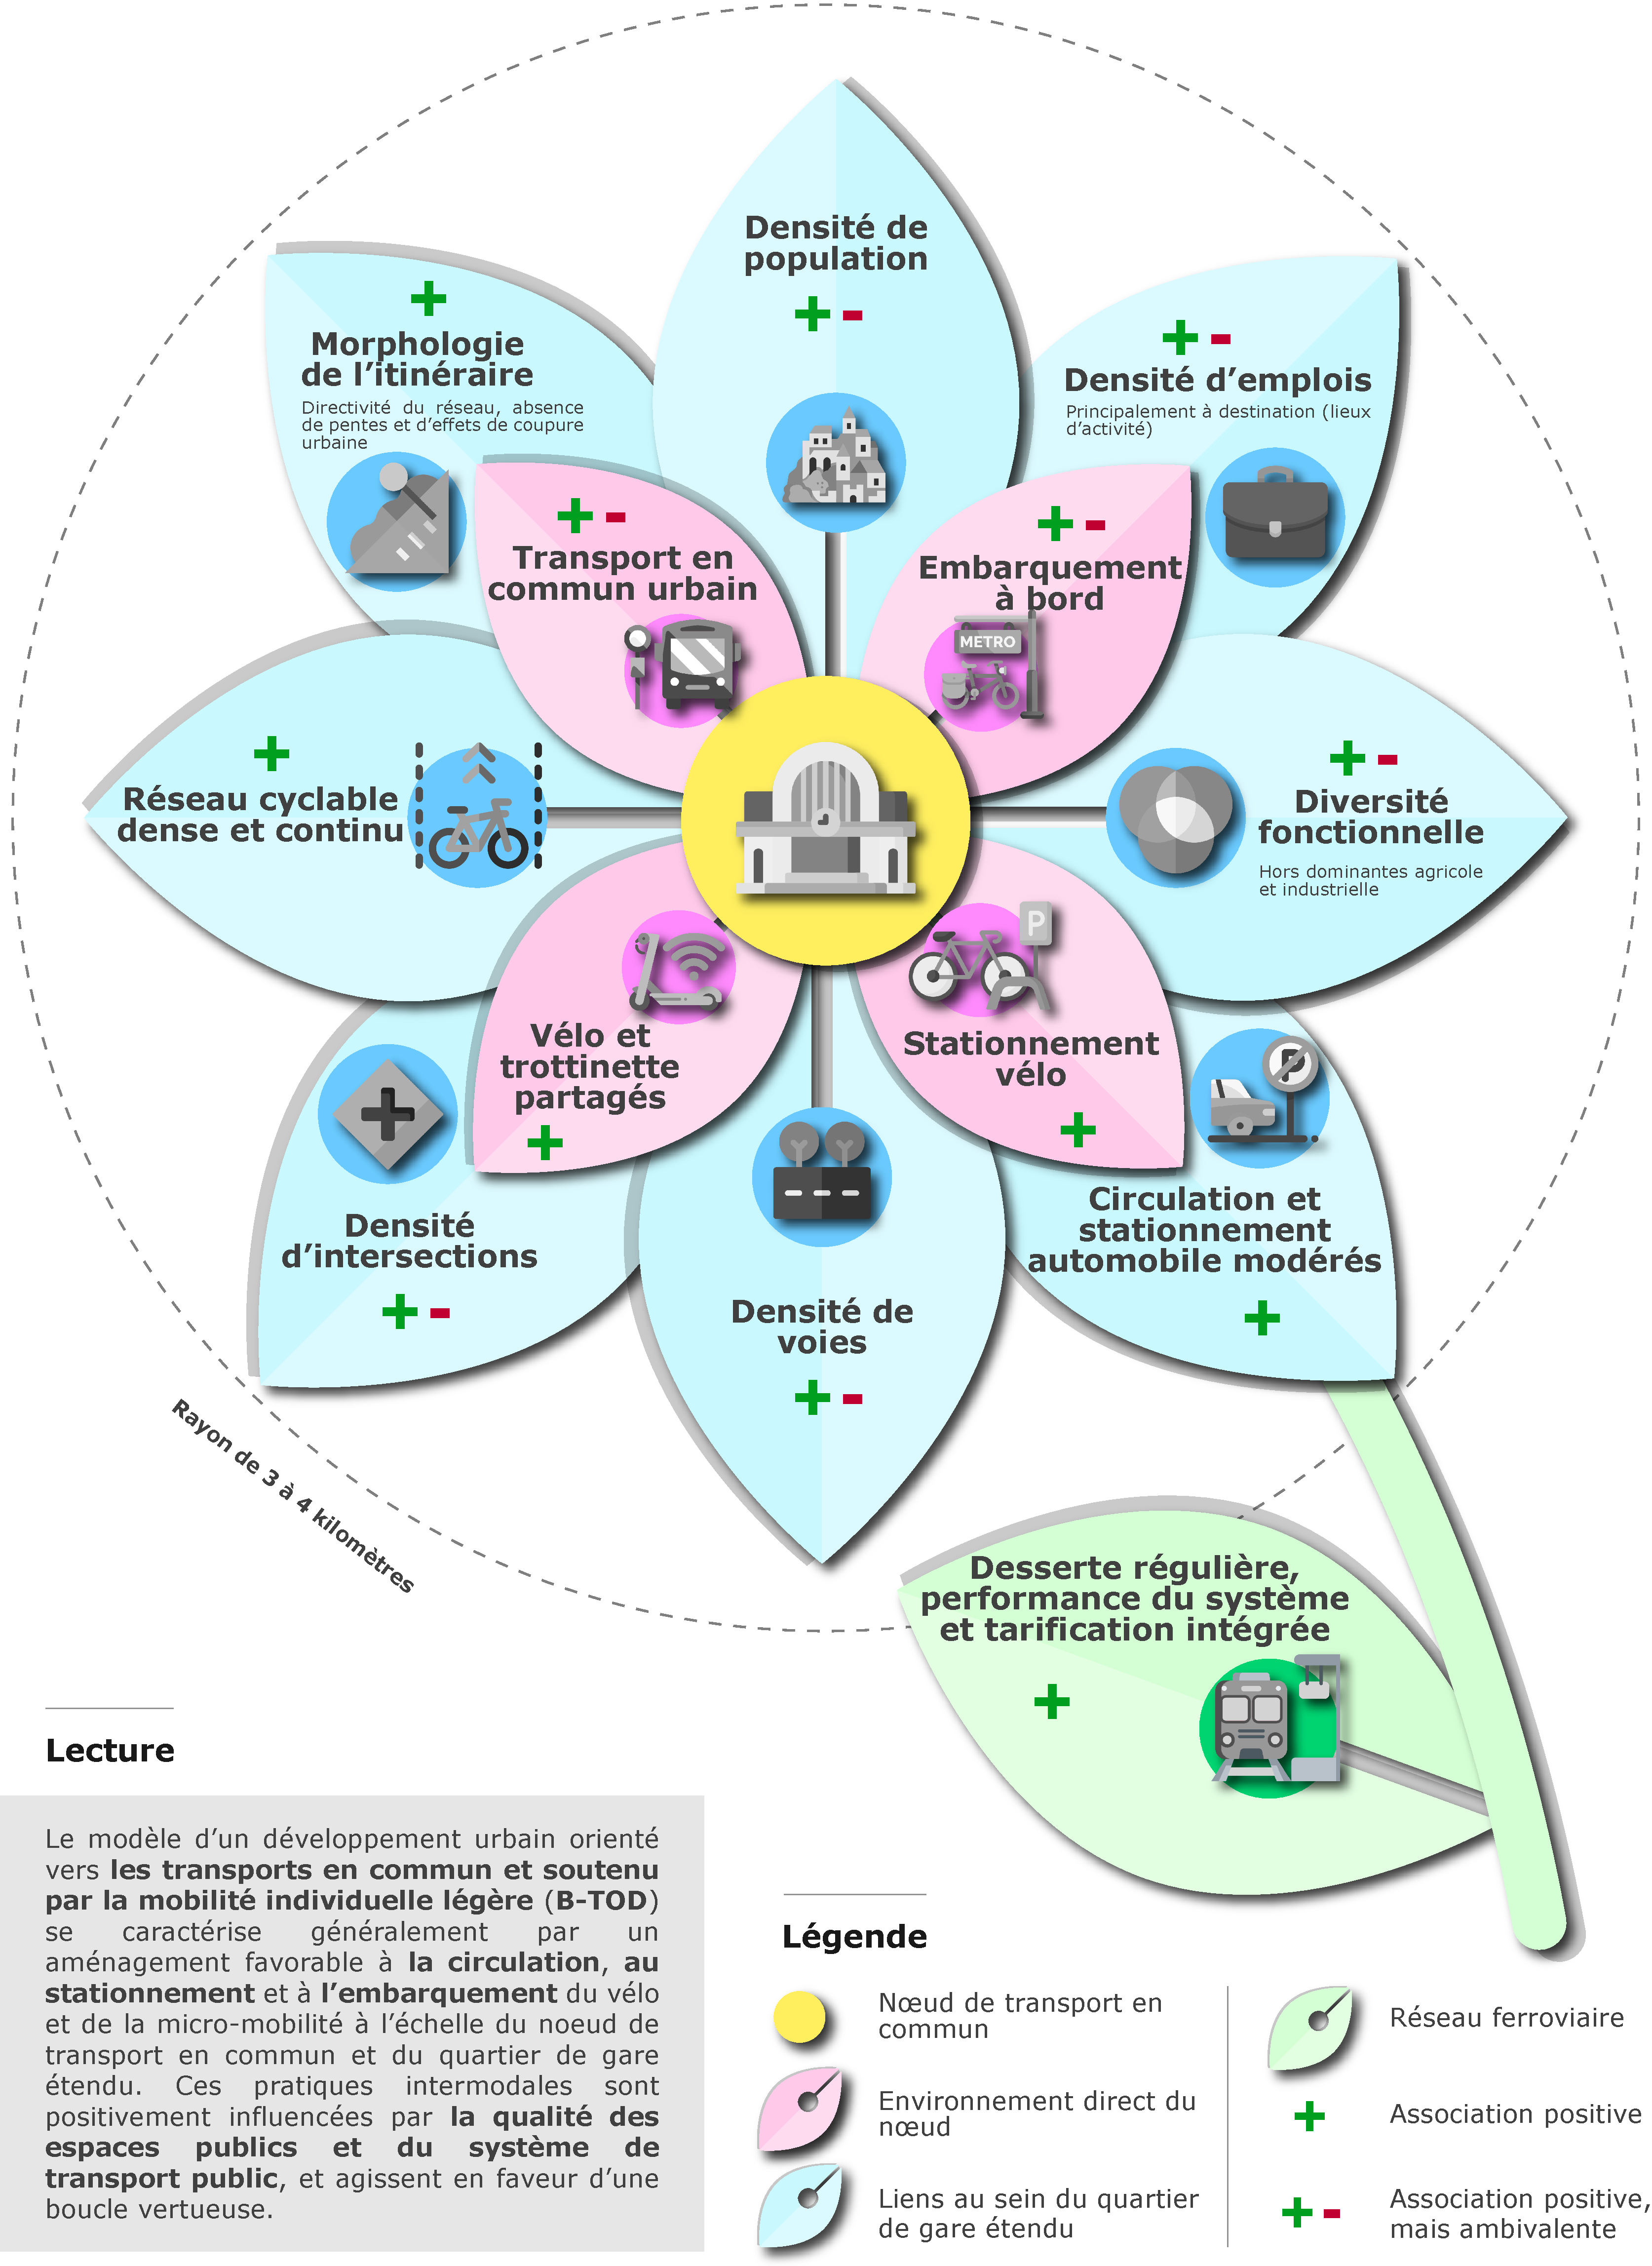
\includegraphics[width=1\columnwidth]{src/Figures/Chap-2/FR_RSL_Fleur_TOD.pdf}}
        \vspace{5pt}
        \begin{flushright}\scriptsize{
        Auteur~: \textcolor{blue}{Dylan Moinse (2023)}
        }\end{flushright}
    \end{figure}
    
    % Objectifs
En réponse aux questionnements de recherche formulés dans la \hyperref[chap2:formulation-questions-recherche]{sous-section~1.1} (page~\pageref{chap2:formulation-questions-recherche}), l'objectif de cette \acrshort{RSL} réside dans l'ambition d'approfondir et d'étendre la compréhension des connaissances relatives au \acrshort{M-TOD}. Ce travail a visé à identifier clairement les facteurs qui facilitent ou entravent l'adoption de ce modèle d'urbanisme. Dans cette perspective, l'analyse développée dans ce chapitre s'est appuyée sur un ensemble de six questions de recherche, qui ont constitué le cadre directeur de notre étude. Ces interrogations se concentrent sur l'interaction entre les dynamiques urbaines, les politiques publiques et leur rôle dans l'intégration de la mobilité individuelle légère au sein des systèmes de transport en commun, ainsi que sur l'influence de ces pratiques sur les configurations territoriales. L'examen détaillé de la littérature a mis en exergue l'importance capitale des \acrshort{7Ds} et des comportements de mobilité, offrant ainsi une perspective plus nuancée et détaillée de ces déplacements et de leurs implications bénéfiques dans l'élaboration d'un modèle urbain qui promeut un système de mobilité et d'urbanisme \gls{durable} et viable. Il est ressorti de cette étude que l'aire d'influence étendue des gares offre des gains d'accessibilité à un plus grand nombre de voyageur·se·s potentiel·le·s. De ce fait, nous pouvons nous référer à la notion de \Guillemets{potentiel d'accueil des territoires} \textcolor{blue}{\autocite[86]{kaufmann_retour_2014}}\index{Kaufmann, Vincent|pagebf} comme un élément moteur et soutenu par ces pratiques de mobilité, en lien avec les principes du \acrshort{TOD}. Pour conclure, la dernière question de recherche aborde les défis auxquels est confronté ce modèle d'urbanisme émergent, interrogeant notamment les lacunes actuelles dans la littérature scientifique face à une production récente des connaissances en lien avec le \acrshort{M-TOD}.%%Rédigé%%

    % 2.*.*.*
    \needspace{1\baselineskip} % Réserve de l'espace
\subsection*{Lacunes dans la littérature scientifique
    \label{chap2:literature-gap}
    }

    % Literature gap : état de la littérature
En guise de transition vers l'examen de notre matériau empirique, nous clôturons ce chapitre en soulevant les principaux enjeux qui nous paraissent encore peu abordés en relation avec le concept de \acrshort{M-TOD}. L'analyse bibliométrique opérée dans le cadre de notre \acrshort{RSL} a permis de mettre en évidence diverses lacunes se rapportant aux contours de notre sujet de recherche. Il convient de souligner, en premier lieu, une sous-représentation des recherches considérant certaines formes de mobilité individuelle légère. En dépit de l'intérêt croissant pour \acrshort{VLS}, le \acrshort{VFF} et la \acrshort{TEFF} depuis 2018, les études portant sur la trottinette et le vélo pliant, qu'ils soient électriques ou non motorisés, demeurent relativement rares. Cette observation s'accompagne d'une focalisation sur les systèmes de transport en commun urbains, laissant supposer un potentiel encore peu exploré du rôle des réseaux ferroviaires structurants à l'échelle régionale en association avec les nouvelles formes de mobilité. En outre, nous constatons que la littérature scientifique et technique s'attache peu à une approche systémique de l'ensemble du système de mobilité collective d'une zone géographique donnée, une démarche pourtant cruciale pour appréhender l'intermodalité-voyageur·se·s de manière systémique. De surcroît, le paysage scientifique actuel révèle un déséquilibre géographique, avec une prédominance des études ayant pour contexte géographique une agglomération internationale ou régionale en Chine, aux États-Unis et aux Pays-Bas. Finalement, l'examen des cadres géographiques étudiés révèle une tendance marquée à privilégier les échelles intercommunale et communale, tandis que les travaux de recherche adoptant une échelle régionale se révèlent être exceptionnels.%%Rédigé%%

    % Literature gap : concepts et méthodes
Au regard des cadres théoriques définis, nous avons pu identifier une disparité intéressante entre la mention fréquente et l'exploitation du concept de \acrshort{TOD} dans la littérature scientifique et la quasi-absence de sa réadaptation sous le nom de \acrshort{M-TOD}. En ce qui concerne les méthodes de recherche employées, nous notons une proportion majoritaire d'études prenant appui sur les bases de données ouvertes ou privées issues de l'\textsl{Open Data} et de la \textsl{Big Data}. Par ailleurs, les techniques d'enquête par questionnaire, entretien ou observation, généralement plus adaptées aux terrains de taille intermédiaire, sont néanmoins tout aussi présentes selon les contextes géographiques, notamment en Europe. Notons cependant l'insuffisance des approches qualitatives et plus largement des recherches mixtes, en particulier en ce qui concernant les options de mobilité individuelle légère émergentes. Le regard porté sur les méthodes d'analyse suggère une forte inclination pour l'emploi de la modélisation et des statistiques descriptives ainsi que pour l'usage du \acrshort{SIG}.%%Rédigé%%

    % Literature gap : résultats
L'analyse détaillée du corpus construit pour cette \acrshort{RSL} a révélé non seulement l'existence de disparités dans l'exploitation des \acrshort{7Ds} en lien avec le \acrshort{M-TOD}, mais a aussi conduit au développement de nouveaux questionnements issus de la confrontation des études empiriques :
    \begin{customitemize}
\item Quel est l'impact, direct ou indirect, de la densité démographique sur les configurations territoriales et les pratiques de mobilité favorisées par le modèle urbain du \acrshort{M-TOD}~?
\item La notion de mixité sociale est-elle complémentaire avec les principes promus par le \acrshort{M-TOD}~?
\item Les différentes formes de combinaison modale induisent-elles des besoins spécifiques en termes d'infrastructures et d'aménagements cyclables~?
\item Quels sont les gains d'accessibilité offerts par l'intégration de la mobilité individuelle légère au sein des systèmes de transport en commun~?
\item Comment l'aire d'influence des nœuds de transport en commun varie-t-elle en fonction de la nature des combinaisons modales, des différentes étapes du déplacement intermodal, ainsi que des facteurs environnementaux et socio-démographiques~?
\item Dans quelle mesure la performance des réseaux de transport en commun et la gestion de l'espace dédié à l'automobile contribuent-elles à une meilleure articulation entre formes urbaines et comportements de mobilité~?
\item Le \acrshort{M-TOD} peut-il être considéré comme un facteur exacerbant les inégalités d'accès à la mobilité~?
\item Ce modèle urbain peut-il intégrer la mobilité liée aux loisirs, aux rencontres sociales ou aux promenades (\textsl{undirected travel})~?
\item La démocratisation de l'adoption de la mobilité individuelle légère en intermodalité peut-elle former un cercle vertueux influençant les formes urbaines, lesquelles, à leur tour, modèlent les comportements de mobilité~?
    \end{customitemize}%%Rédigé%%

    % Enjeux
Au gré des défis soulevés par la littérature scientifique concernant la conception d'un système urbain orienté vers le développement des réseaux de transport en commun hybridé à l'intégration de la mobilité individuelle légère, la thèse de doctorat aspire à mieux saisir les clés de compréhension du concept de \acrshort{M-TOD}. Le présent chapitre a souligné la nécessité d'élargir le champ de recherche à ce sujet pour inclure une variété accrue de formes de mobilité et de niveaux d'analyse géographique, dans le but d'enrichir notre appréhension de cette stratégie d'aménagement, réinterprétée sous l'angle de la mobilité individuelle légère. Ces observations nous conduisent à une réflexion sur l'adoption d'une approche géostatistique conjuguée à une démarche qualitative susceptibles de livrer des perspectives plus nuancées sur les comportements et les expériences de mobilité des individus.%%Rédigé%%

    % Structure de la thèse
Dans cette perspective, notre recherche doctorale s'articule autour de l'exploration d'un espace géographique européen à une échelle régionale, avec un intérêt particulier porté sur l'ensemble du réseau de mobilité, essentiellement structuré autour des réseaux ferroviaires. Le prochain \hyperref[chap3:titre]{chapitre} (page~\pageref{chap3:titre}) sera consacré à la délimitation du périmètre géographique de l'étude et à la présentation de notre méthodologie, laquelle se compose d'une enquête de terrain. L'objectif de cette démarche mixte est de saisir le développement des pratiques intermodales qui associent l'usage des transports en commun et des options émergentes de mobilité individuelle légère, et de les examiner sous l'angle des comportements de mobilité et de leurs interactions avec l'environnement urbain (voir le \hyperref[chap4:titre]{chapitre~4}, page~\pageref{chap4:titre}). La détermination d'un groupe social de cyclo-voyageur·se·s activement présent dans les divers territoires examinés nous permettra d'interroger leurs interactions dans le contexte de quartiers de gare élargis, en mobilisant la notion d'accessibilité intermodale (voir le \hyperref[chap5:titre]{chapitre~5}, page~\pageref{chap5:titre}). Cette approche géographique des distances nous conduira à proposer un modèle fondé sur un indice nœud-lieu (\textsl{Node-Place Index}), visant à évaluer le potentiel de développement urbain en synergie avec un système de mobilité alternative à l'échelle régionale, dans le \hyperref[chap6:titre]{chapitre~6} (page~\pageref{chap6:titre}).%%Rédigé%%

% ___________________________________________
     \newpage
     
% Valorisation scientifique
    \begin{tcolorbox}[colback=white!5!white,
                      colframe=blue!75!blue,
                      title=Valorisation scientifique
                      \\
                      Chapitre~2]
\Large{\textbf{\textcolor{blue}{Chapitre d'ouvrage collectif~:}}}
    \\\\
\small{\textcolor{blue}{\textcite{moinse_systematic_2023}}\index{Moinse, Dylan|pagebf}. \foreignlanguage{english}{\textsl{A Systematic Literature Review on Station Area Integrating Micromobility in Europe: A 21\textsuperscript{st} Century Transit-Oriented Development}}. In: Belaïd,~F., Arora,~A. (eds) \textsl{Smart Cities. Studies in Energy, Resource and Environmental Economics}. Springer, Cham. ISBN: 978-3-031-35663-6 (p.~171-204).
\\
\footnotesize{\url{https://doi.org/10.1007/978-3-031-35664-3_12}} (\textbf{OS})}
    \end{tcolorbox}

    % ___________________________________________
    % Sous-bibliographie
    \newpage
    \sectionheader{Sous-bibliographie du chapitre~2}
    \begingroup
    \renewcommand{\bibfont}{\scriptsize}
\printbibliography[segment=\therefsegment, heading=subbibintoc, title={Sous-bibliographie du chapitre~2}, label=chap2:bibliographie]
    \endgroup
    \end{refsegment}